% Options for packages loaded elsewhere
% Options for packages loaded elsewhere
\PassOptionsToPackage{unicode}{hyperref}
\PassOptionsToPackage{hyphens}{url}
\PassOptionsToPackage{dvipsnames,svgnames,x11names}{xcolor}
%
\documentclass[
  spanish,
  letterpaper,
  DIV=11,
  numbers=noendperiod]{scrreprt}
\usepackage{xcolor}
\usepackage{amsmath,amssymb}
\setcounter{secnumdepth}{5}
\usepackage{iftex}
\ifPDFTeX
  \usepackage[T1]{fontenc}
  \usepackage[utf8]{inputenc}
  \usepackage{textcomp} % provide euro and other symbols
\else % if luatex or xetex
  \usepackage{unicode-math} % this also loads fontspec
  \defaultfontfeatures{Scale=MatchLowercase}
  \defaultfontfeatures[\rmfamily]{Ligatures=TeX,Scale=1}
\fi
\usepackage{lmodern}
\ifPDFTeX\else
  % xetex/luatex font selection
\fi
% Use upquote if available, for straight quotes in verbatim environments
\IfFileExists{upquote.sty}{\usepackage{upquote}}{}
\IfFileExists{microtype.sty}{% use microtype if available
  \usepackage[]{microtype}
  \UseMicrotypeSet[protrusion]{basicmath} % disable protrusion for tt fonts
}{}
\makeatletter
\@ifundefined{KOMAClassName}{% if non-KOMA class
  \IfFileExists{parskip.sty}{%
    \usepackage{parskip}
  }{% else
    \setlength{\parindent}{0pt}
    \setlength{\parskip}{6pt plus 2pt minus 1pt}}
}{% if KOMA class
  \KOMAoptions{parskip=half}}
\makeatother
% Make \paragraph and \subparagraph free-standing
\makeatletter
\ifx\paragraph\undefined\else
  \let\oldparagraph\paragraph
  \renewcommand{\paragraph}{
    \@ifstar
      \xxxParagraphStar
      \xxxParagraphNoStar
  }
  \newcommand{\xxxParagraphStar}[1]{\oldparagraph*{#1}\mbox{}}
  \newcommand{\xxxParagraphNoStar}[1]{\oldparagraph{#1}\mbox{}}
\fi
\ifx\subparagraph\undefined\else
  \let\oldsubparagraph\subparagraph
  \renewcommand{\subparagraph}{
    \@ifstar
      \xxxSubParagraphStar
      \xxxSubParagraphNoStar
  }
  \newcommand{\xxxSubParagraphStar}[1]{\oldsubparagraph*{#1}\mbox{}}
  \newcommand{\xxxSubParagraphNoStar}[1]{\oldsubparagraph{#1}\mbox{}}
\fi
\makeatother


\usepackage{longtable,booktabs,array}
\usepackage{calc} % for calculating minipage widths
% Correct order of tables after \paragraph or \subparagraph
\usepackage{etoolbox}
\makeatletter
\patchcmd\longtable{\par}{\if@noskipsec\mbox{}\fi\par}{}{}
\makeatother
% Allow footnotes in longtable head/foot
\IfFileExists{footnotehyper.sty}{\usepackage{footnotehyper}}{\usepackage{footnote}}
\makesavenoteenv{longtable}
\usepackage{graphicx}
\makeatletter
\newsavebox\pandoc@box
\newcommand*\pandocbounded[1]{% scales image to fit in text height/width
  \sbox\pandoc@box{#1}%
  \Gscale@div\@tempa{\textheight}{\dimexpr\ht\pandoc@box+\dp\pandoc@box\relax}%
  \Gscale@div\@tempb{\linewidth}{\wd\pandoc@box}%
  \ifdim\@tempb\p@<\@tempa\p@\let\@tempa\@tempb\fi% select the smaller of both
  \ifdim\@tempa\p@<\p@\scalebox{\@tempa}{\usebox\pandoc@box}%
  \else\usebox{\pandoc@box}%
  \fi%
}
% Set default figure placement to htbp
\def\fps@figure{htbp}
\makeatother


% definitions for citeproc citations
\NewDocumentCommand\citeproctext{}{}
\NewDocumentCommand\citeproc{mm}{%
  \begingroup\def\citeproctext{#2}\cite{#1}\endgroup}
\makeatletter
 % allow citations to break across lines
 \let\@cite@ofmt\@firstofone
 % avoid brackets around text for \cite:
 \def\@biblabel#1{}
 \def\@cite#1#2{{#1\if@tempswa , #2\fi}}
\makeatother
\newlength{\cslhangindent}
\setlength{\cslhangindent}{1.5em}
\newlength{\csllabelwidth}
\setlength{\csllabelwidth}{3em}
\newenvironment{CSLReferences}[2] % #1 hanging-indent, #2 entry-spacing
 {\begin{list}{}{%
  \setlength{\itemindent}{0pt}
  \setlength{\leftmargin}{0pt}
  \setlength{\parsep}{0pt}
  % turn on hanging indent if param 1 is 1
  \ifodd #1
   \setlength{\leftmargin}{\cslhangindent}
   \setlength{\itemindent}{-1\cslhangindent}
  \fi
  % set entry spacing
  \setlength{\itemsep}{#2\baselineskip}}}
 {\end{list}}
\usepackage{calc}
\newcommand{\CSLBlock}[1]{\hfill\break\parbox[t]{\linewidth}{\strut\ignorespaces#1\strut}}
\newcommand{\CSLLeftMargin}[1]{\parbox[t]{\csllabelwidth}{\strut#1\strut}}
\newcommand{\CSLRightInline}[1]{\parbox[t]{\linewidth - \csllabelwidth}{\strut#1\strut}}
\newcommand{\CSLIndent}[1]{\hspace{\cslhangindent}#1}

\ifLuaTeX
\usepackage[bidi=basic]{babel}
\else
\usepackage[bidi=default]{babel}
\fi
% get rid of language-specific shorthands (see #6817):
\let\LanguageShortHands\languageshorthands
\def\languageshorthands#1{}


\setlength{\emergencystretch}{3em} % prevent overfull lines

\providecommand{\tightlist}{%
  \setlength{\itemsep}{0pt}\setlength{\parskip}{0pt}}



 


\KOMAoption{captions}{tableheading}
\makeatletter
\@ifpackageloaded{tcolorbox}{}{\usepackage[skins,breakable]{tcolorbox}}
\@ifpackageloaded{fontawesome5}{}{\usepackage{fontawesome5}}
\definecolor{quarto-callout-color}{HTML}{909090}
\definecolor{quarto-callout-note-color}{HTML}{0758E5}
\definecolor{quarto-callout-important-color}{HTML}{CC1914}
\definecolor{quarto-callout-warning-color}{HTML}{EB9113}
\definecolor{quarto-callout-tip-color}{HTML}{00A047}
\definecolor{quarto-callout-caution-color}{HTML}{FC5300}
\definecolor{quarto-callout-color-frame}{HTML}{acacac}
\definecolor{quarto-callout-note-color-frame}{HTML}{4582ec}
\definecolor{quarto-callout-important-color-frame}{HTML}{d9534f}
\definecolor{quarto-callout-warning-color-frame}{HTML}{f0ad4e}
\definecolor{quarto-callout-tip-color-frame}{HTML}{02b875}
\definecolor{quarto-callout-caution-color-frame}{HTML}{fd7e14}
\makeatother
\makeatletter
\@ifpackageloaded{bookmark}{}{\usepackage{bookmark}}
\makeatother
\makeatletter
\@ifpackageloaded{caption}{}{\usepackage{caption}}
\AtBeginDocument{%
\ifdefined\contentsname
  \renewcommand*\contentsname{Tabla de contenidos}
\else
  \newcommand\contentsname{Tabla de contenidos}
\fi
\ifdefined\listfigurename
  \renewcommand*\listfigurename{Listado de Figuras}
\else
  \newcommand\listfigurename{Listado de Figuras}
\fi
\ifdefined\listtablename
  \renewcommand*\listtablename{Listado de Tablas}
\else
  \newcommand\listtablename{Listado de Tablas}
\fi
\ifdefined\figurename
  \renewcommand*\figurename{Figura}
\else
  \newcommand\figurename{Figura}
\fi
\ifdefined\tablename
  \renewcommand*\tablename{Tabla}
\else
  \newcommand\tablename{Tabla}
\fi
}
\@ifpackageloaded{float}{}{\usepackage{float}}
\floatstyle{ruled}
\@ifundefined{c@chapter}{\newfloat{codelisting}{h}{lop}}{\newfloat{codelisting}{h}{lop}[chapter]}
\floatname{codelisting}{Listado}
\newcommand*\listoflistings{\listof{codelisting}{Listado de Listados}}
\makeatother
\makeatletter
\makeatother
\makeatletter
\@ifpackageloaded{caption}{}{\usepackage{caption}}
\@ifpackageloaded{subcaption}{}{\usepackage{subcaption}}
\makeatother
\usepackage{bookmark}
\IfFileExists{xurl.sty}{\usepackage{xurl}}{} % add URL line breaks if available
\urlstyle{same}
\hypersetup{
  pdftitle={Criminología: una introducción},
  pdfauthor={Juanjo Medina y Lorea Arenas (Coordinadores)},
  pdflang={es},
  colorlinks=true,
  linkcolor={blue},
  filecolor={Maroon},
  citecolor={Blue},
  urlcolor={Blue},
  pdfcreator={LaTeX via pandoc}}


\title{Criminología: una introducción}
\author{Juanjo Medina y Lorea Arenas (Coordinadores)}
\date{2025-08-21}
\begin{document}
\maketitle

\renewcommand*\contentsname{Tabla de contenidos}
{
\hypersetup{linkcolor=}
\setcounter{tocdepth}{2}
\tableofcontents
}

\bookmarksetup{startatroot}

\chapter*{Bienvenida}\label{bienvenida}
\addcontentsline{toc}{chapter}{Bienvenida}

\markboth{Bienvenida}{Bienvenida}

Esta es la página web de ``Criminología: una introducción''. Este es un
libro de texto digital en formato abierto y gratuito que está siendo
redactado por varios expertos en la materia y que aspira a servir de
manual de referencia en las asignaturas de introducción a la
criminología que se imparten en los distintos grados universitarios de
criminología en España.

El libro se distribuye bajo una licencia
\href{https://creativecommons.org/licenses/by-nc-nd/4.0/deed.en}{CC
BY-NC-ND 4.0} y ha sido producido usando
\href{https://quarto.org/}{Quarto}.

\begin{tcolorbox}[enhanced jigsaw, bottomtitle=1mm, toprule=.15mm, colbacktitle=quarto-callout-note-color!10!white, bottomrule=.15mm, leftrule=.75mm, colframe=quarto-callout-note-color-frame, opacitybacktitle=0.6, titlerule=0mm, breakable, colback=white, left=2mm, arc=.35mm, title=\textcolor{quarto-callout-note-color}{\faInfo}\hspace{0.5em}{Nota}, toptitle=1mm, coltitle=black, rightrule=.15mm, opacityback=0]

Una licencia Creative Commons solo es válida cuando la aplica la persona
o entidad que posee los derechos sobre la obra protegida. Las obras
pueden contener componentes (por ejemplo, fotografías, ilustraciones o
citas) a los que el titular de los derechos de la obra no puede aplicar
la licencia. En última instancia, es responsabilidad del lector evaluar
de forma independiente el estado de los derechos de autor de cualquier
obra o componente de una obra que utilice, teniendo en cuenta el uso que
le vaya a dar

\end{tcolorbox}

Esta es una página en construcción. El libro, o al menos una parte
sustancial del mismo, no estará disponible hasta septiembre del 2026. Si
tenéis sugerencias sobre el volumen podéis escribir a jmedina11@us.es.

\bookmarksetup{startatroot}

\chapter*{Preliminares}\label{preliminares}
\addcontentsline{toc}{chapter}{Preliminares}

\markboth{Preliminares}{Preliminares}

\section*{Coordinación y autoría}\label{coordinaciuxf3n-y-autoruxeda}
\addcontentsline{toc}{section}{Coordinación y autoría}

\markright{Coordinación y autoría}

\begin{itemize}
\item
  \textbf{Coordinación}: Juanjo Medina y Lorea Arenas
\item
  \textbf{Autoría}:

  \begin{itemize}
  \item
    Juanjo Medina (\emph{Universidad de Sevilla}): capítulos 1, 2, 4, 5,
    6, 8, 9, 10, 13, 15 y 15
  \item
    Lorea Arenas (\emph{Universidad de Extremadura}): capítulos 4, 7 y
    14
  \item
    Raquel Bartolomé (\emph{Universidad de Castilla-La Mancha}):
    capítulo 11
  \item
    Elisa García España (\emph{Universidad de Málaga}): capítulo 12
  \item
    Jonathan Torres (Universidad de Sevilla): capítulo 3
  \end{itemize}
\end{itemize}

\section*{Plan de trabajo}\label{plan-de-trabajo}
\addcontentsline{toc}{section}{Plan de trabajo}

\markright{Plan de trabajo}

El plan es intentar tener borradores preliminares del capítulo sobre
concepto, delincuentes, delito, respuestas estatales, clase social, y
política antes de finalizar el 2025.

Nuestra aspiración es tener la mayor parte del volumen terminado en
septiembre del 2026, listo para ser usado en el primer semestre del
curso 2026/2027, aunque es posible que algún capítulo se retrase hasta
finales del 2026.

Estamos en proceso de garantizar el uso de todas las imágenes empleadas.
Algunas de ellas no presentan problemas, para el uso legítimo de otras
aún estamos en fase de tramitar los permisos necesarios.

La apariencia de las imágenes también es algo que tenemos que optimizar.
Somos conscientes de que su apariencia varía dependiendo de si se emplea
un teléfono u otro tipo de dispositivo. Para poder corregir esto tenemos
que programar esta parte del libro directamente en \emph{html} y esto es
algo un poco más trabajoso que solamente haremos más adelante.

\section*{¿Por qué este libro?}\label{por-quuxe9-este-libro}
\addcontentsline{toc}{section}{¿Por qué este libro?}

\markright{¿Por qué este libro?}

Los grados de criminología en España son una titulación relativamente
reciente y, a diferencia de lo que ocurre en países de habla inglesa, el
mercado de los libros de texto en castellano que sirvan para nutrir de
contenido a las distintas asignaturas que conforman estos grados no está
tan desarrollado como sería deseable. Para algunas asignaturas
simplemente no existen manuales que puedan usarse, mientras que para
otras algo más de competencia y posibilidad de elección es algo que
alumnos y docentes probablemente considerarían apropiado.

Uno pensaría que la introducción a la criminología, una asignatura
generalmente de primero de carrera y fundamental en el itinerario
formativo de nuestros estudiantes, sería una excepción a esta norma,
pero nuestra tesis es que no, que los manuales al uso en nuestro país no
satisfacen del todo las necesidades formativas para asignaturas de
introducción a la criminología.

Quitando manuales ya muy viejunos, en España si eres profesor de una
introducción a la criminología tienes básicamente dos opciones: los
principios de criminología de Redondo y Garrido (2023) o la introducción
de Larrauri (2020) . Por más que estos dos volumenes tienen muchas
virtudes a nosotras como docentes nos plantean una serie de
limitaciones.

\begin{figure}

\begin{minipage}{0.50\linewidth}
\pandocbounded{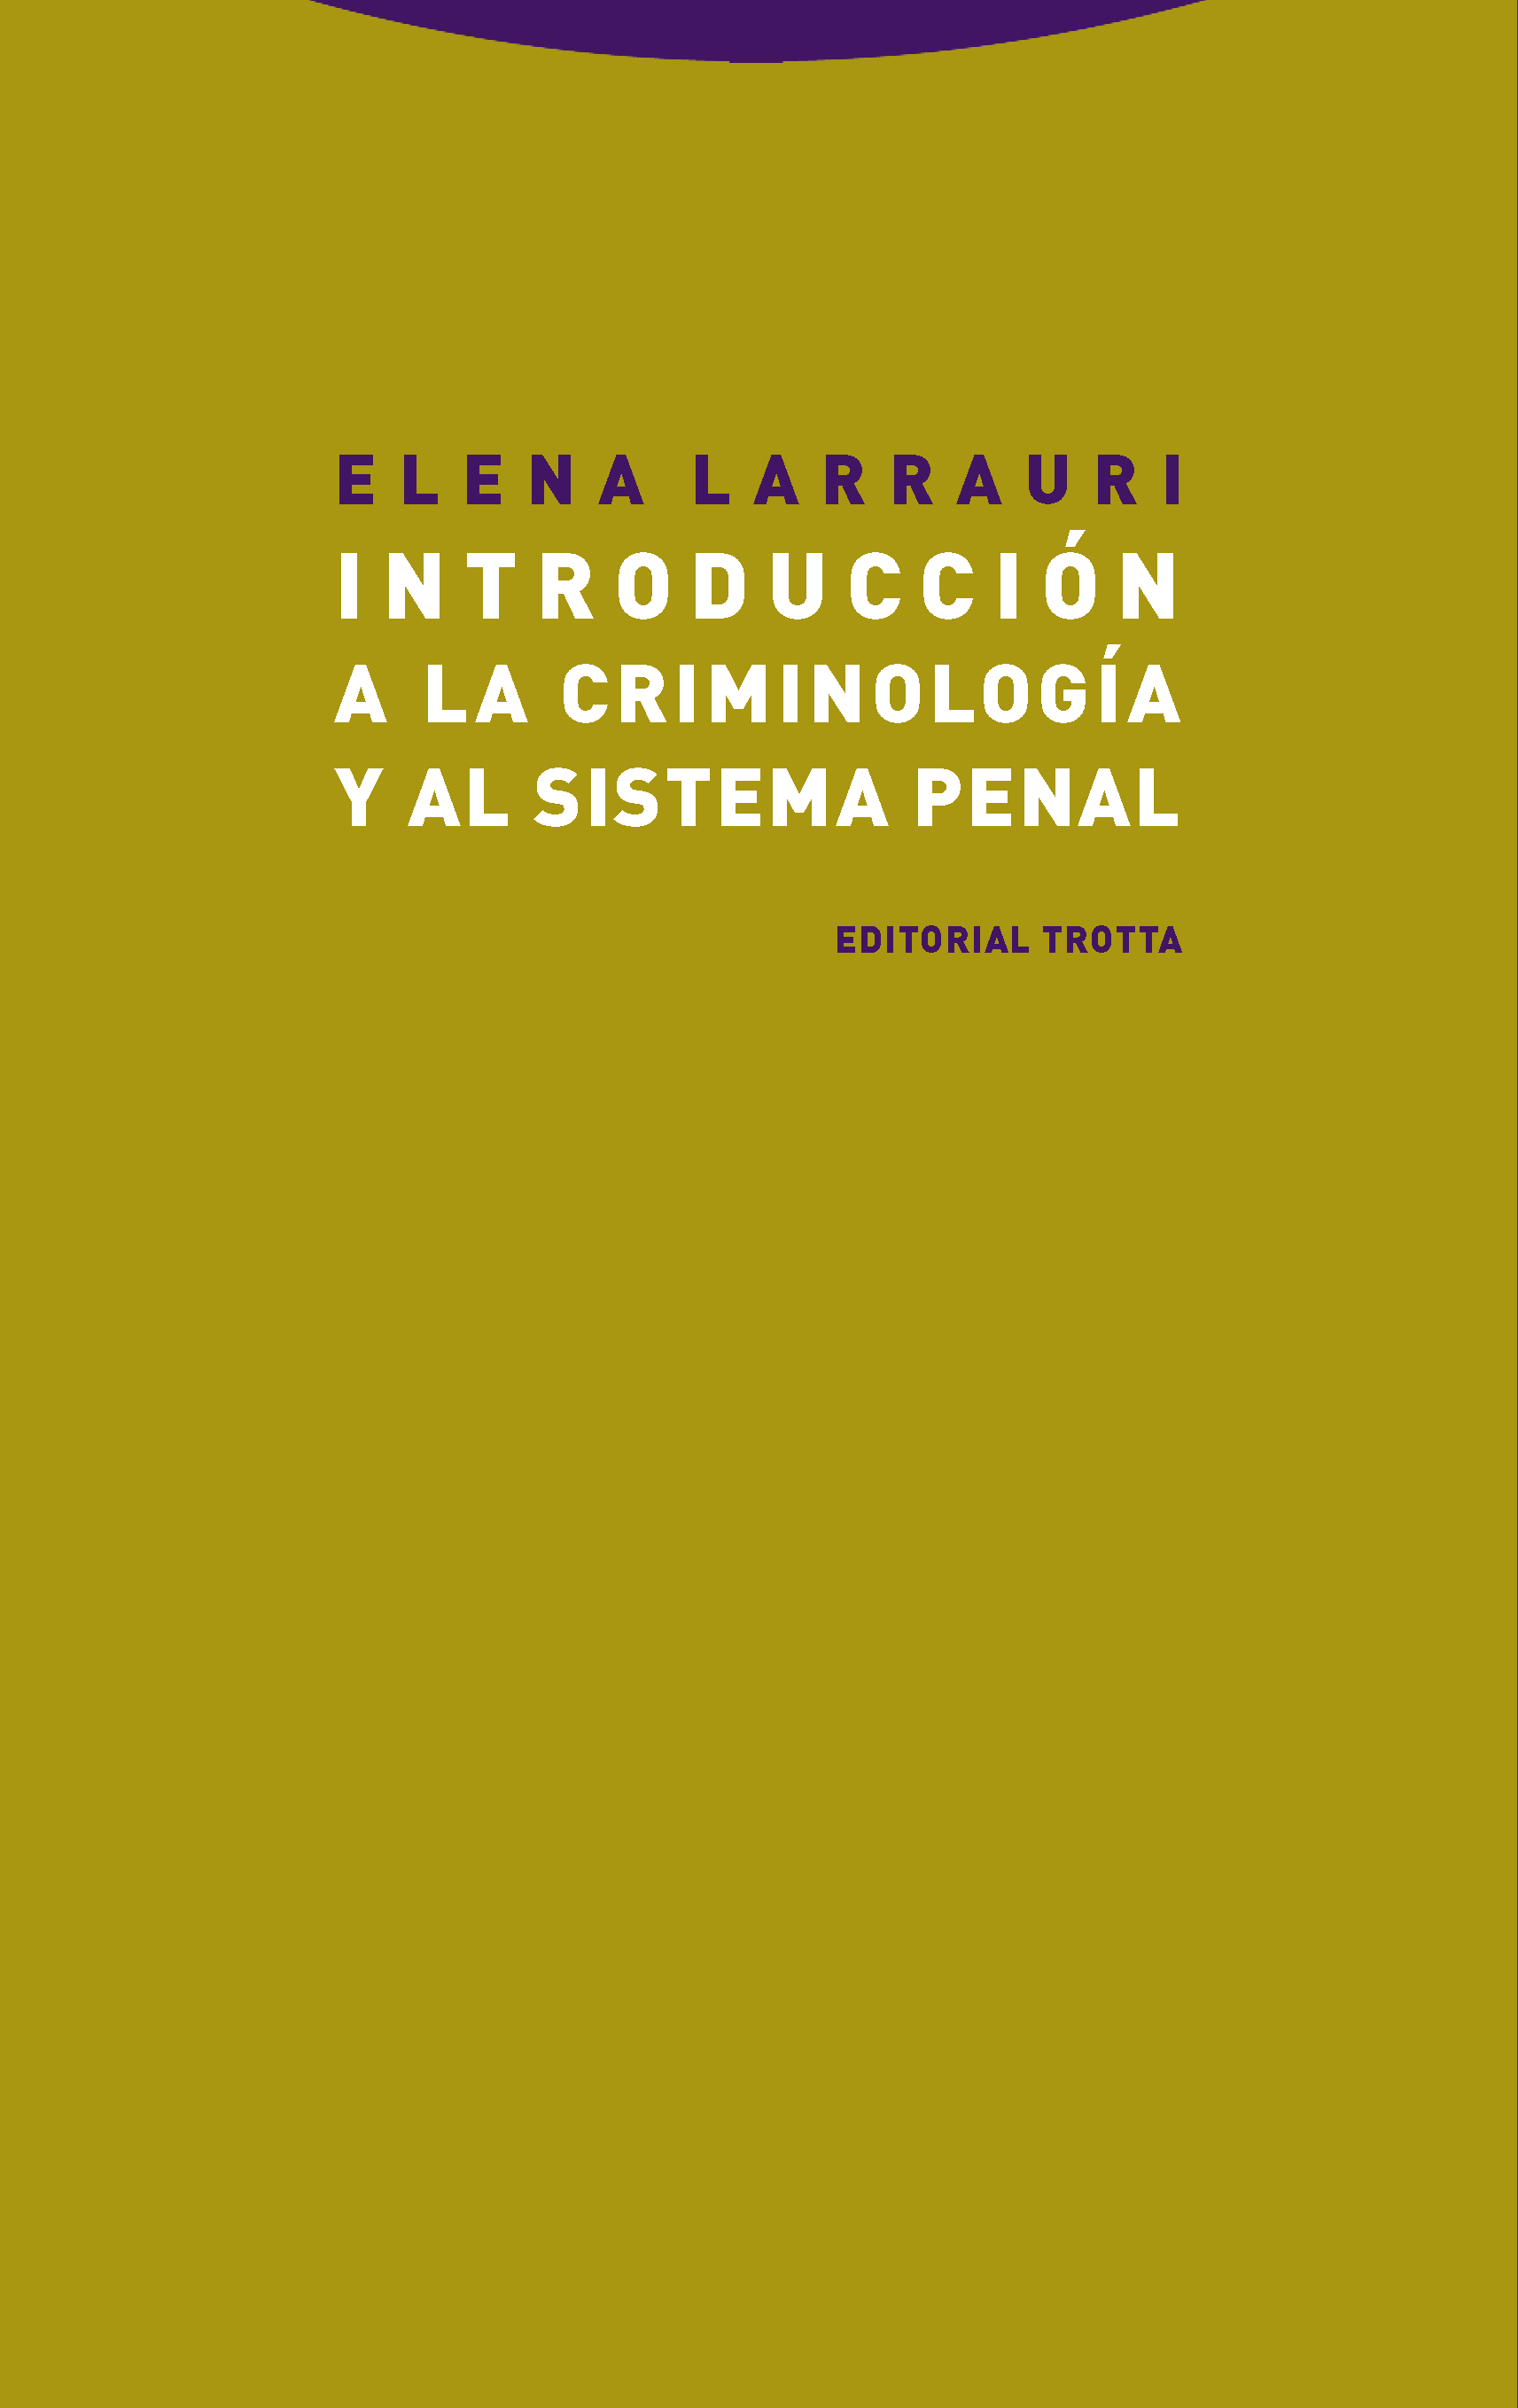
\includegraphics[keepaspectratio]{images/introduccion.png}}\end{minipage}%
%
\begin{minipage}{0.50\linewidth}
\pandocbounded{
\includegraphics[keepaspectratio]{images/larrauri.jpeg}}\end{minipage}%
\newline
\begin{minipage}{0.50\linewidth}
Elena Larrauri y su manual\end{minipage}%

\end{figure}%

El manual de Larrauri (2020) aspira a dar una introducción moderna y
ajustada al hecho de que esta suele ser una asignatura del primer
semestre de primero. Nuestro principal problema con este manual es que,
por más que nos gusta, se nos queda corto, sobre todo si tenemos en
cuenta que tiene dos partes, una que puede valer para una introducción a
la criminología (con unas cien páginas) y otra que más bien es una
introducción al sistema de justicia penal o al control penal (que en
numerosos planes de estudios es una asignatura diferente también de
primero).

\begin{figure}

\begin{minipage}{0.33\linewidth}
\pandocbounded{
\includegraphics[keepaspectratio]{images/santiago_redondo.jpg}}\end{minipage}%
%
\begin{minipage}{0.33\linewidth}
\pandocbounded{
\includegraphics[keepaspectratio]{images/garrido.jpg}}\end{minipage}%
%
\begin{minipage}{0.33\linewidth}
\pandocbounded{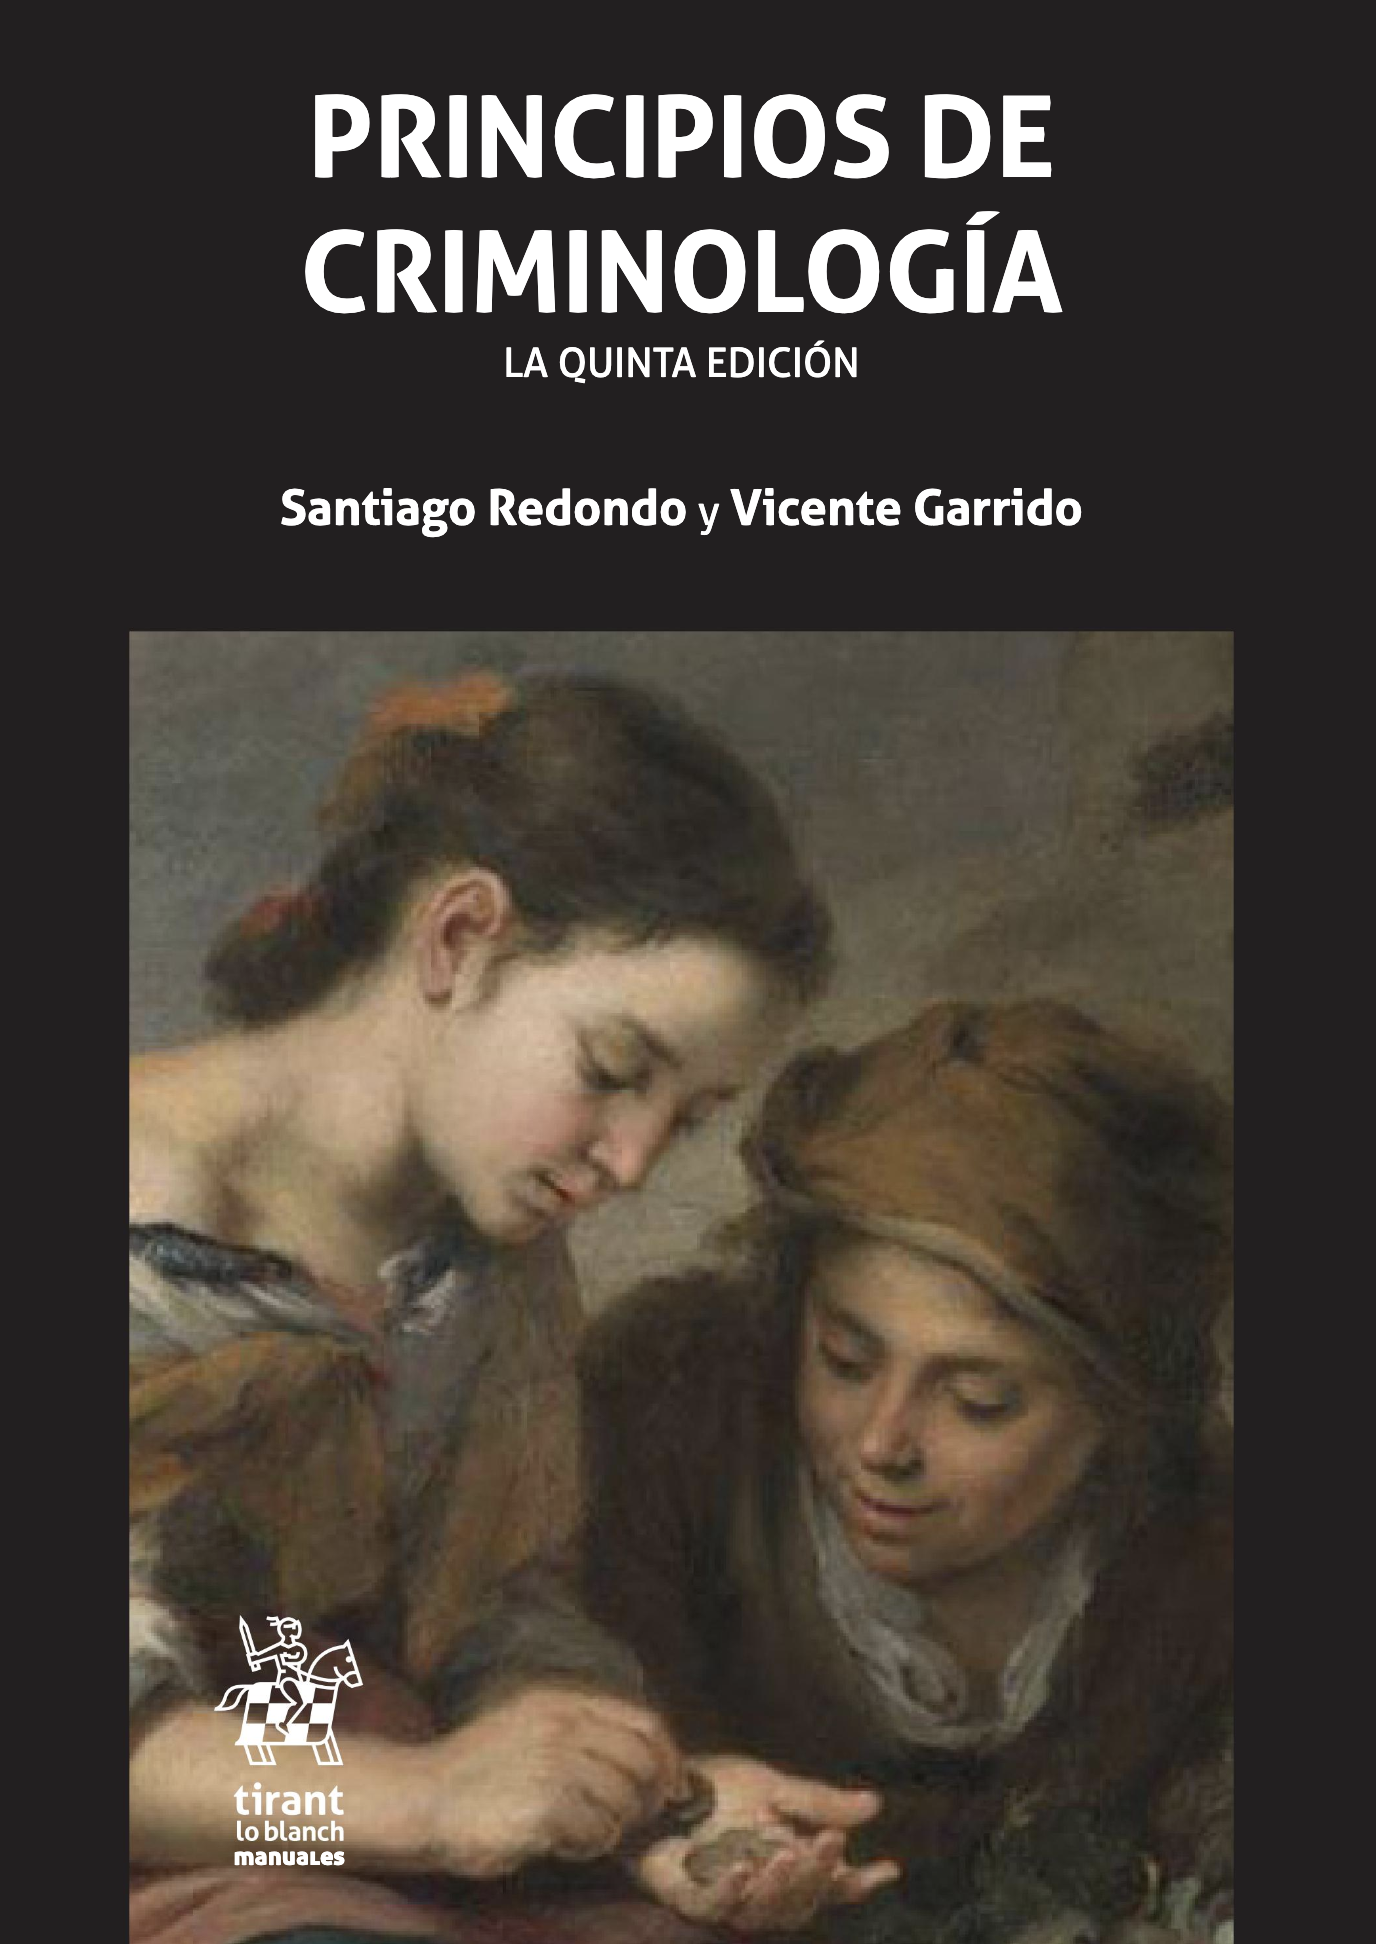
\includegraphics[keepaspectratio]{images/principios.png}}\end{minipage}%
\newline
\begin{minipage}{0.33\linewidth}
Santiago Redondo y Vicente Garrido\end{minipage}%

\end{figure}%

Con más de 800 páginas los Principios de Criminología de Santiago
Redondo y Vicente Garrido cortos no son. Nuestro problema con este
manual es que una parte muy notable del mismo es más bien un manual para
teoría criminológica y la otra parte también muy notable lo es para
asignaturas de lo que se suele llamar en los grados \emph{Formas
especiales de criminalidad}. Por tanto, lo que queda del manual para una
introducción a la criminología es más restringido de lo que esas 800 y
pico páginas pueden sugerir.

En resumen, son dos excelentes manuales, pero queremos usar este texto
para reivindicar también un temario diferenciado para las asignaturas de
introducción, que no sean, como en otros manuales que no citamos aquí,
en realidad y de forma exclusiva una introducción a la teoría
criminológica. Es inevitable hablar de teoría en una asignatura de
introducción, pero no podemos llevarlo hasta el punto de restar
autonomía o sentido a estas asignaturas de introduccion a la disciplina.

Al margen de estas cuestiones, cada libro es también un reflejo de las
preferencias teóricas, disciplinares, metodológicas e incluso políticas
e ideológicas de quienes los escriben. En ese sentido, pensamos que
generar una tercera opción a estos manuales mencionados puede dar una
mayor libertad de elección tanto al profesorado como al alumnado.

Este libro además aspira a ser gratuito y de código abierto, además de
dinámico. La publicación científica se ha convertido en un negocio para
unas cuantas editoriales internacionales que exprimen recursos
económicos de estudiantes, administraciones públicas, y universidades.
Nosotros creemos en otro modelo de ciencia, uno que la concibe como un
bien común que debería estar al alcance de todos \footnote{Para una
  discusión del concepto del bien común aplicado a la publicación
  académica ver Moore (2025).}, no solamente de quienes pueden
permitirse pagar por ella.

Una de las ventajas de publicar en este formato digital y susceptible al
cambio continuo es que probablemente se ira renovando y modificando de
una forma más contínua que si fuera un libro de texto al uso. Su versión
digital tendrá este carácter dinámico más flexible y abierto. Una vez
estemos satisfechos con un primer borrador final generaremos un enlace
para que quien quiera pueda descargarse e imprimir este texto en formato
pdf. La versión en pdf probablemente solamente la actualizaremos de
forma anual, por lo que es posible que en ocasiones se puedan apreciar
algunas diferencias entre la versión digital y la version susceptible de
impresión como fichero pdf.

\section*{Convenciones}\label{convenciones}
\addcontentsline{toc}{section}{Convenciones}

\markright{Convenciones}

A lo largo del texto se incluiran citas de trabajos originales en
numerosas ocasiones de textos escritos en inglés. Para facilitar la
lectura y comprensión estas citas, cuando se inserten en el texto
principal, serán traducidas al castellano por los autores del volumen.

También a lo largo del texto apareceran ``notas'' con una apariencia
visual como la siguiente:

\begin{tcolorbox}[enhanced jigsaw, bottomtitle=1mm, toprule=.15mm, colbacktitle=quarto-callout-note-color!10!white, bottomrule=.15mm, leftrule=.75mm, colframe=quarto-callout-note-color-frame, opacitybacktitle=0.6, titlerule=0mm, breakable, colback=white, left=2mm, arc=.35mm, title=\textcolor{quarto-callout-note-color}{\faInfo}\hspace{0.5em}{Nota}, toptitle=1mm, coltitle=black, rightrule=.15mm, opacityback=0]

\textbf{¿Que son las notas?}

Estas notas son simplemente pequeños excursos, aclaraciones o
expansiones de algunas ideas que pueden ser leidas para complementar el
argumento principal del texto.

\end{tcolorbox}

\part{Introducción}

\chapter{¿Qué es la criminología?}\label{quuxe9-es-la-criminologuxeda}

\section{Definiendo la
criminología}\label{definiendo-la-criminologuxeda}

Si estás leyendo estas líneas deberías tener una idea de cómo responder
esta pregunta, pues este es un libro escrito para estudiantes de
criminología a los que se les debe asumir un mínimo conocimiento sobre
de qué va la titulación que han elegido. Pero esas ideas pueden estar
contaminadas por relatos públicos que existen sobre la criminología que
no se corresponden con la realidad.

Cuando, siendo más joven, iba a alguna fiesta y me preguntaban a qué me
dedicaba, me costaba la misma vida decir que era criminólogo porque
sabía cómo iba a acabar la conversación. Generalmente la cosa derivaba
hacia las imágenes que el público tiene sobre los criminólogas y lo
excitante que tiene que ser capturar a un delincuente. Hollywood, la
industria del entretenimiento en general, tiene buena parte de la culpa
de esos mitos que existen sobre la criminología. A veces en películas y
series televisivas se introducen personajes que dicen ser criminólogos
cuando en realidad son otra cosa. A veces eso se debe a un problema de
traducción del inglés al español, otras veces es desconocimiento de los
guionistas. No son criminólogas quienes se dedican a hacer perfiles
sobre delincuentes en serie para ayudar a su captura, generalmente son
psicólogas forenses. Tampoco son criminólogos quienes se dedican a
recopilar y analizar pruebas que puedan servir a consolidar la evidencia
probatoria en un juicio para condenar a alguien; suelen ser
criminalistas, esto es personas con una carrera técnica (medicina,
biología, informática, química, etc.) que pueden aportar sus
conocimientos para estos fines y que suelen contar con algún tipo de
formación especializada en policía científica. Las criminólogas son otra
cosa.

¿Qué es, entonces, la criminología? Podría parecer una pregunta sencilla
merecedora de una respuesta simple. Como veremos en realidad existen
muchas formas de practicar y entender la criminología, que además han
variado históricamente y entre distintos países, por lo que existen
distintas formas de responder. No existe tampoco un consenso universal
sobre las fronteras de la criminología (dónde empieza y dónde termina) y
sobre cuál es su legítimo objeto de estudio. Veremos también que hay
distintas formas de entender las relaciones de la criminología con otras
disciplinas científicas y su carácter distintivo, así como con sus
relaciones en el campo de la práctica profesional, las instituciones de
la justicia penal y la administración pública, el activismo social, y el
campo de la política.

El eminente criminólogo norteamericano Edwin Sutherland, autor de uno de
los más influyentes manuales de criminología del siglo XX, definía la
criminología como:

\begin{quote}
``el conjunto de conocimientos sobre el delito como fenómeno social.
Incluye en su ámbito los procesos de elaboración de leyes, de infracción
de leyes y de reacción ante la infracción de leyes. Estos procesos son
tres aspectos de una secuencia de interacciones algo unificada. Ciertos
actos que se consideran indeseables son definidos por las normas
políticas. A pesar de esta limitación, algunas personas persisten en ese
comportamiento y, por lo tanto, cometen delitos; la sociedad política
reacciona con castigos u otros tratamientos, o con medidas preventivas.
Esta secuencia de interacciones es el objeto de estudio de la
criminología.'' (Sutherland 1947, 1).
\end{quote}

\begin{figure}

\begin{minipage}{0.50\linewidth}
\pandocbounded{
\includegraphics[keepaspectratio]{images/sutherland.jpeg}}\end{minipage}%
%
\begin{minipage}{0.50\linewidth}
El sociólogo estadounidense Edwin Sutherland (1883-1950)\end{minipage}%

\end{figure}%

En manuales españoles más modernos, como el de la profesora Larrauri
(2020), se da a entender que la criminología es una ciencia social que
obtiene sus conocimientos de la observación y análisis de la realidad de
la delincuencia y del funcionamiento del sistema penal. Y de una forma
parecida Redondo y Garrido (2023, p.) definen la criminología como
aquella ``ciencia que estudia los comportamientos delictivos y las
reacciones sociales frente a ellos''. Ambas son formulaciones resumidas
de lo propuesto por Edwin Sutherland. Por su parte, y con la elegancia y
sofisticación que lo suele caracterizar, el escocés David Garland
caracteriza a la criminología de la siguiente forma:

\begin{quote}
``Interpreto la criminología como un género específico de discurso e
investigación sobre el delito -- un género que se desarrolló durante la
modernidad y que puede ser distinguido de otras formas de hablar y
pensar sobre la conducta criminal. Así, por ejemplo, la pretensión de la
criminología de ser una empresa científica basada en el análisis
empírico la separa de los discursos morales y jurídico legales, mientras
que su atención hacia el delito la diferencia de otros géneros
científico sociales, como la sociología de la desviación y el control,
cuyo objeto de estudio es más amplio y no se encuentra definido por el
Código Penal. Desde mediados del siglo XX, la criminología de forma
creciente ha venido a estar marcada de otros discursos por los adornos
de una identidad distintiva, con sus revistas, asociaciones
profesionales, cátedras, e institutos de investigación'' (Garland 2002a,
8)
\end{quote}

Lo primero que tenéis que entender es que no hay nada sagrado o escrito
en piedra sobre estas definiciones. Como en muchas otras cuestiones en
las ciencias sociales tendréis que juzgar por vosotras mismas lo
convincentes que son los argumentos para mantener una postura u otra. El
hecho de que haya distintas interpretaciones o respuestas implica que es
una cuestión contestada, y que no podemos considerar del todo cerrada.
No obstante, podéis ver que hay elementos comunes en estas
caracterizaciones.

Dado que esta es una introducción a la materia no podemos simplemente
dejaros con la idea de que ``hay muchas formas de entender la
criminología, vosotros veréis cuál elegís.'' Vamos a daros una
descripción personal preliminar que utilizaremos en este manual y luego
iremos destilando y justificando sus partes. La criminología, para
nosotras, puede caracterizarse como:

\begin{quote}
un proyecto intelectual y académico que se ha ido institucionalizando de
forma gradual, desigual, y creciente en distintos países como disciplina
o campo de estudio con un desarrollo socialmente determinado entroncado
en las ciencias sociales, e interconectado de forma radical con varias
disciplinas que tiene como temas de reflexión e investigación: el delito
como evento, las personas y organizaciones que cometen delitos, las
personas que sufren el delito, y las respuestas socioculturales,
políticas, e institucionales al mismo que hace todo esto desde una
perspectiva plural, aunque históricamente desarrollada por hombres
occidentales y blancos (con los sesgos y puntos ciegos que ello implica)
y que al tratar de estas cuestiones es un cuerpo de conocimientos y
prácticas sociales con consecuencias en la vida de las personas y la
sociedad que hace imposible no considerar su naturaleza política
\end{quote}

\subsection{La criminología como proyecto intelectual y
académico}\label{la-criminologuxeda-como-proyecto-intelectual-y-acaduxe9mico}

Quizás hayáis notado que hablamos de la criminología como proyecto
intelectual y académico, un término más amplio, en lugar de ciencia,
como hacen la mayoría de otros manuales. Esto es algo que tiene que ver
con debates que existen sobre cuál es la naturaleza legítima del
conocimiento criminológico. La razón por la que preferimos esta
terminología es porque creemos que es más generosa con las distintas
formas de hacer criminología y más abierta a capturar y aceptar las
distintas almas de la criminología.

Y es que en las ciencias sociales han coexistido, desde el siglo XIX,
dos culturas, dos formas de entenderlas. Una tendencia ha sido acercarse
a las humanidades, mientras que otra ha tendido más a un acercamiento a
las ciencias naturales. Han coexistido, no de forma pacífica, una forma
de conocer el mundo (lo que en términos técnicos se denomina
epistemología) \textbf{idiográfica} - que ha destacado la particularidad
de todo fenómeno social, la utilidad limitada de las generalizaciones, y
la necesidad de la comprensión empática -- con una forma de conocer el
mundo \textbf{nomotética} -que ha destacado el paralelismo entre los
procesos humanos y sociales con los procesos materiales y ha buscado el
desarrollo de leyes universales que se puedan aplicar al mundo social.

Como destaca Wallerstein (2004, 19) las ciencias sociales han sido como
``alguien atado a dos caballos galopando en dirección contraria''. David
Smith (2014) resume bien esta situación dentro de la criminología
europea:

\begin{quote}
``De un lado se encuentran quienes usan el lenguaje y los métodos de la
ciencia, mientras que en el otro se encuentran quienes usan el lenguaje
y los métodos de las humanidades. Hasta cierto grado, estas dos
perspectivas están ligadas a distintas disciplinas académicas'' (que
contribuyen a la criminología) ``pero en algunas instancias representan
divisiones dentro de disciplinas establecidas. Así, en el campo de la
ciencia están las contribuciones que proceden de la epidemiología, la
genética, buena parte de la psiquiatría, la psicología social y
experimental, casi toda la economía, y toda sociología que trabaja con
estadísticas oficiales y encuestas. En el campo de las humanidades se
encuentran buena parte de la sociología, historia, teoría política, la
mayoría de los estudios sobre medios de comunicación, y la teoría
psicoanalítica. Mientras que disciplinas como la antropología social se
encuentran a medio camino. El campo de las ciencias tiene afinidad con
la filosofía analítica, mientras que el campo de las humanidades tiene
mayor afinidad con la filosofía continental. Hace 20 años el campo de
las humanidades (no el de las ciencias) estaba muy influenciado por el
marxismo o la teoría crítica, aunque estas influencias han
disminuido\ldots{} Este esquema es una simplificación muy cruda que
exagera el contraste y hay autores que se sitúan entre ambos campos. No
obstante, es importante tenerla en cuenta porque sirve como una guía
útil para mapear la criminología, dado que se corresponde con diferentes
métodos de investigación y concepciones de lo que es el conocimiento
criminológico. Los que van de científicos usan números, estadísticas,
encuestas y experimentos controlados, mientras que quienes se acercan a
las humanidades describen eventos particulares y ejemplos singulares en
toda su complejidad, insistiendo en matices y detalles (en contrapunto
con la idea científica de ``precisión'').'' (Smith 2014, p.)
\end{quote}

Pensamos, teniendo esto en cuenta, que definir la criminología como
ciencia parece una forma de posicionarse frente a estas dos formas de
entenderla. De hecho, cuando lees determinados autores y la forma en que
definen la criminología como ciencia parece que esa es precisamente la
intención. Parecería que es una forma de decir que solo el alma
``cientificista'' de la criminología que ha buscado acercarse al modelo
de las ciencias naturales (y que en ocasiones puede representar los
intereses del status quo) es la correcta o la adecuada. Creemos que
adoptar esta postura es problemática a nivel normativo (es decir como
objetivo a seguir) y a nivel descriptivo (de definir nuestro campo a día
de hoy). A nivel normativo es empobrecedor: creemos que ambos enfoques,
el cientificista y el que se aproxima a las humanidades tienen mucho que
ofrecer para generar conocimiento enriquecedor. Y a nivel descriptivo no
reflejaría bien la pluralidad de enfoques que coexisten dentro de la
criminología como organización o fenómeno social. De ahí, que prefiramos
esta terminología (proyecto intelectual y académico) como más inclusiva.

\begin{tcolorbox}[enhanced jigsaw, bottomtitle=1mm, toprule=.15mm, colbacktitle=quarto-callout-note-color!10!white, bottomrule=.15mm, leftrule=.75mm, colframe=quarto-callout-note-color-frame, opacitybacktitle=0.6, titlerule=0mm, breakable, colback=white, left=2mm, arc=.35mm, title=\textcolor{quarto-callout-note-color}{\faInfo}\hspace{0.5em}{Nota}, toptitle=1mm, coltitle=black, rightrule=.15mm, opacityback=0]

\textbf{¿Es la criminología una profesión?}

Una consecuencia de caracterizar la criminología como proyecto
intelectual y académico es que tenemos que definir a un criminólogo o
criminóloga como cualquier investigador(a) académico(a) que se ha
especializado de forma demonstrable en los objetos de estudio de la
criminología, con independencia de su titulación.

No estamos la criminología como una profesión, como un conjunto de
ocupaciones cerradas a personas graduadas en criminología. El debate
sobre si la criminología es una profesión solo lo hemos visto planteado
en España (aunque es posible que se de en otros países con un legado
cultural como el nuestro). La razón de ello tiene que ver con la manía
que tenemos en nuestro país de encasillar y encorsetar (legal y
administrativamente) todo, así como con el engranaje legal de nuestro
mercado laboral. Ni en el mundo anglosajón ni en Europa central y del
norte vamos a encontrar este tipo de debates. Sonaría a marciano.

Sin entrar en debates sobre conceptos sociológicos y teóricos de lo que
es una profesión, podemos preguntarnos si hay alguna ocupación laboral
que solamente un graduado en criminología podría realizar. La respuesta,
en nuestra opinión, es un no categórico y rotundo. De entrada, la
formación universitaria no es FP, tiene una ambición diferente. Creemos
que las titulaciones en criminología deberían capacitar a sus egresados
para desarrollar un amplio espectro de ocupaciones laborales en el campo
de la respuesta al delito, pero no creemos que esta capacitación los
pone en una situación que les permita levantar murallas sobre
determinadas ocupaciones que solamente ellos (los titulados o las
tituladas en criminología) podrían o deberían realizar. En cuanto uno
profundiza un poco sobre las habilidades, conocimientos y capacidades de
cualquier ocupación laboral que los egresados en criminología quisieran
monopolizar se vería que en realidad personas con otras titulaciones
también desarrollan, o pueden desarrollar, dichas habilidades,
conocimientos y capacidades de forma experta. No hay, por tanto, ninguna
ocupación laboral que defina de forma específica al criminólogo. Aunque
es verdad, al mismo tiempo, que su formación debería ponerles en una
cierta ventaja competitiva o, cuanto menos facilitarles el acceso, en
relación con distintas ocupaciones laborales en el ámbito de la
seguridad, la prevención, y la intervención frente al delito tanto en el
ámbito público como en el privado. En este sentido la persona con
conocimientos criminológicos debería, como mínimo, estar capacitada
para:

\begin{itemize}
\item
  desarrollar diagnósticos sobre el fenómeno criminal en un determinado
  marco espacio temporal;
\item
  evaluar y gestionar los riesgos y necesidades de intervención de
  víctimas y delincuentes;
\item
  desarrollar mapas de riesgo y vulnerabilidades en el sector público y
  privado;
\item
  diseñar, implementar y evaluar programas de detección y prevención de
  la delincuencia en contextos institucionales o comunitarios;
\item
  analizar, evaluar y desarrollar propuestas de políticas públicas en
  materia de delincuencia y seguridad.
\end{itemize}

Otra cosa es que los planes de estudio de los grados de criminología
doten al alumnado de estas capacidades de forma adecuada. Ocurre, por
seguir con el debate que nos anima, que en España funcionamos, por un
lado, con una institución de origen feudal que son los colegios
profesionales que aspiran a defender intereses corporativos creados y a
monopolizar para los egresados en determinadas titulaciones ciertas
ocupaciones. Y, por otro lado, contamos con una administración pública
que a la hora de hacer convocatorias públicas y de definir sus
plantillas laborales lo hace sobre esquemas generados en diálogo y
negociación competitiva con estos colegios profesionales. Sucede también
que la criminología en España es una recién llegada en esta fiesta y los
colegios profesionales ligados a otras titulaciones nos llevan ventaja y
han levantado barreras para que los egresados en criminología puedan
trabajar en determinados espacios de la administración pública.

En ese sentido, aunque no creo que la criminología sea una profesión en
el sentido aquí indicado, todo egresado en criminología interesado en la
promoción profesional de su titulación debería luchar por la creación en
su comunidad autónoma de un colegio profesional y colegiarse en dichos
órganos para poder reivindicar de forma colectiva y más efectiva un
mercado laboral más justo para quienes se especializan en este ámbito
disciplinar.

Pero sería un error de bulto que en los colegios profesionales
empezáramos a pensar que hay que entrar al juego de levantar barreras. O
que acabaran creyendose que un criminólogo o criminóloga solo lo es la
persona a la que, por virtud de su titulación, se le permite colegiarse.
Eso iría en contra de lo que se deriva de entender la criminología como
un proyecto intelectual y académico abierto a cualquier disciplina
científica, algo que no es simplemente un deseo normativo sino una
descripción fáctica de la realidad.

\end{tcolorbox}

\subsection{La institucionalización de la
criminología}\label{la-institucionalizaciuxf3n-de-la-criminologuxeda}

Señalamos en nuestra propuesta que la criminología se ha ido
institucionalizando de forma gradual, desigual, y creciente en distintos
países como disciplina o campo de estudio. Entender que es la
criminología puede ser más fácil si entendemos algo sobre su historia. Y
también si clarificamos que es eso de una ``disciplina''. Parafraseando
al sociólogo Immanuel Wallerstein (2004) una disciplina es tres cosas de
forma simultánea: categoría intelectual, estructura institucional, y
cultura. Una disciplina:

\begin{quote}
``es una categoría intelectual, una forma de afirmar que existe un campo
determinado de estudio con algún tipo de fronteras (por más que sean
disputadas, con otras disciplinas, o ambiguas) y con modos consensuados
de hacer investigación de una forma legítima\ldots{} Son construcciones
sociales cuyos orígenes han de ser situados en las dinámicas del sistema
histórico que les dan forma'' (Wallerstein 2004, 166).
\end{quote}

Es decir, son creaciones humanas definidas socialmente y que, para
entender, como veremos también a continuación, hay que analizar también
como objeto de análisis social e histórico (¿Por qué surgen cuando
surgen? ¿Quién se beneficia de su aparición? ¿Por qué adoptan la forma
que adoptan? ¿Cuáles son sus consecuencias sociales?).

\begin{quote}
``Las disciplinas son también estructuras institucionales con formas más
elaboradas desde finales del siglo XIX'' (Wallerstein 2004, 166).
\end{quote}

Estas estructuras y elementos que dotan de institucionalidad a la
criminología son, por ejemplo, los departamentos universitarios, grados
y otras titulaciones universitarias, revistas especializadas, sociedades
científicas nacionales e internacionales, colecciones bibliográficas
especializadas, premios ligados a la disciplina, congresos y
convenciones periódicas, etc. Son el cemento que da concreción a la
disciplina como categoría intelectual, ``los adornos que dotan de
identidad distintiva'' a los que se refería David Garland en su
definición.

\begin{quote}
``Finalmente, las disciplinas son culturas. Los investigadores que se
definen como miembros de una disciplina comparten algunas experiencias
comunes. A menudo han leído los mismos libros ´clásicos´. Existen
debates tradicionales bien conocidos dentro de cada disciplina y que son
diferentes de los que existen en otras disciplinas. Cada disciplina
favorece ciertas formas de hacer investigación sobre otras y recompensa
a quienes usan los estilos apropiados. Y aunque la cultura puede
cambiar, y de hecho cambia, con el paso del tiempo, en todo momento hay
formas de presentación que es probable que sean más apreciadas por los
miembros de una disciplina que de los de otra disciplina'' (Wallerstein
2004, 166-67).
\end{quote}

La criminología ha adquirido los rasgos institucionales propios de una
disciplina de forma relativamente reciente, sobre todo en España y en
Europa. Uno de los vectores definitorios de la criminología en la
actualidad es, sin duda, el notable crecimiento que ha experimentado en
las últimas décadas.

\begin{tcolorbox}[enhanced jigsaw, bottomtitle=1mm, toprule=.15mm, colbacktitle=quarto-callout-note-color!10!white, bottomrule=.15mm, leftrule=.75mm, colframe=quarto-callout-note-color-frame, opacitybacktitle=0.6, titlerule=0mm, breakable, colback=white, left=2mm, arc=.35mm, title=\textcolor{quarto-callout-note-color}{\faInfo}\hspace{0.5em}{Nota}, toptitle=1mm, coltitle=black, rightrule=.15mm, opacityback=0]

\textbf{Los titulaciones de criminología en España}

La criminología como titulación universitaria reglada (como grado y
máster oficial) son relativamente recientes. Fuera de nuestras
fronteras, sobre todo en el mundo anglosajón, sí que había estudios
universitarios oficiales sobre criminología desde hace varias décadas.
Por ejemplo, la Escuela de Justicia Criminal de Rutgers University fue
una de las primeras escuelas de criminología en Estados Unidos y fue
fundada en 1974. En España la irrupción y expansión de estas
titulaciones es posterior. Durante los 1990 se produce una proliferación
de títulos propios (no reglados y homologados a nivel nacional) de
criminología (``Expertos Universitarios'') ofrecidos desde Institutos de
Criminología creados prácticamente todos ellos en el seno de
Departamentos de Derecho Penal. Estos títulos de duración variable
atrajeron un amplio número de matriculados y graduados, muchas veces
procedentes del mundo de la policía o de la administración
penitenciaria. Académicos vinculados a estos Institutos de Criminología
-fundamentalmente penalistas, aunque en algunas universidades se
consiguió atraer sobre todo a psicólogos- gestaron la Sociedad Española
de Investigación Criminológica, y contribuyeron al llamado Libro Blanco
de la Criminología. Este Libro Blanco proponía un plan de estudios
consensuado, criticado por su falta de atención a las destrezas
profesionales y el excesivo peso de asignaturas jurídicas (ver Medina
2002), que sirvió de base a la aprobación nacional de una titulación
oficial a nivel nacional en criminología. Este reconocimiento finalmente
llegó en el 2003, inicialmente como una licenciatura de segundo ciclo, y
posteriormente con la aplicación del modelo Bolonia a los grados de 4
años que conocemos hoy. Desde entonces el número de grados de
criminología se multiplicó de forma desmesurada y descontrolada para
saciar una demanda estudiantil exagerada que estaba demasiado
mediatizada por la construcción fantasiosa en la cultura popular de lo
qué es un criminólogo y las nuevas sensibilidades culturales hacia el
delito. La entrada en este mercado de las universidades a distancia y
las universidades privadas contribuyeron aún más a magnificar de forma
probablemente innecesaria, la oferta existente, para explotar esta
demanda exagerada. A fecha de hoy, hay aproximadamente 20332 alumnos
matriculados en grados de criminología (sin contar grados dobles) en
nuestro país repartidos por las 41 universidades públicas y privadas que
ofrecen estos títulos. Por contraponer un ejemplo que creo es relevante,
tan solo hay 6345 alumnos matriculados en sociología repartidos en 16
universidades, todas públicas.

Por otro lado, en España todavía no hay departamentos universitarios de
criminología. Por el contrario, la docencia en los grados de
criminología se reparte entre departamentos diversos (derecho penal,
sociología, psicología de la personalidad, etc.), aunque estas unidades
organizativas, los departamentos de criminología, sí existen en
universidades anglosajonas y europeas.

\end{tcolorbox}

Pero la criminología como espacio de debate e investigación ha precedido
a los grados de especialización en la misma. Así, por ejemplo, aunque no
había grados específicos o departamentos universitarios, sí había
asociaciones profesionales de científicos sociales especializados en el
estudio de la criminología desde los años 1930. La \emph{American
Society of Criminology}, probablemente la más influyente a nivel
internacional, se remonta a 1932 cuando varias personas ligadas al mundo
de la policía comenzaron a reunirse de forma esporádica para debatir
sobre cuestiones relacionadas con temas propios de la criminología,
aunque no fue hasta 1946 que la palabra ``criminología'' aparecía en el
nombre de este grupo (que a lo largo de los años ha ido creciendo y
evolucionando de forma que veremos más adelante).

Muchas de estas asociaciones también han ido desarrollando sus propias
revistas, como \emph{Criminology} (fundada en 1963), la revista oficial
de la Sociedad Americana de Criminología, o el \emph{British Journal of
Criminology} (fundada en 1960) la revista oficial de la \emph{British
Society of Criminology}.

\begin{figure}

\begin{minipage}{0.51\linewidth}
\pandocbounded{
\includegraphics[keepaspectratio]{images/reic.jpg}}\end{minipage}%
%
\begin{minipage}{0.49\linewidth}
\pandocbounded{
\includegraphics[keepaspectratio]{images/bjc.jpeg}}\end{minipage}%
\newline
\begin{minipage}{0.50\linewidth}
Revistas de criminología\end{minipage}%

\end{figure}%

Es importante destacar que, en todo caso, el pensamiento criminológico,
la producción intelectual sobre cuestiones propias de la criminología,
precede también a la creación de instituciones como las sociedades de
criminólogos, sus revistas especializadas, sus departamentos
universitarios, o las titulaciones universitarias en este ámbito - esto
es, los distintos elementos institucionales que aspiran a dotar de una
cierta autonomía organizativa. Hay quienes remontan los orígenes de este
pensamiento al trabajo de autores como Jeremy Bentham (1748-1832) o
Cesare Beccaria (1738-1794) durante el periodo de la Ilustración en el
siglo XVIII. En este sentido, y con independencia de los adornos
institucionales, la criminología como ciencia distintiva o discurso
académico apenas tiene 150 años.

\subsection{La criminología como un producto socialmente
determinado}\label{la-criminologuxeda-como-un-producto-socialmente-determinado}

Tenemos que entender que las disciplinas, en su triple dimensión (como
categorías intelectuales, estructuras institucionales y organización
social, y como cultura) son productos históricos y creaciones humanas
con todas las consecuencias que ello tiene.

No nos debe caber duda que entender e interpretar la criminología y sus
productos nos obliga a entender el contexto en el que opera. Como
señalan Loader y Sparks (2012, 7), parafraseando a Stanley Cohen:

\begin{quote}
``El conocimiento sobre el delito y la justicia no surge de la nada. Ni
está simplemente ubicada en las cabezas y las actividades de quienes lo
producen. La cuestión de qué es lo que viene a conocerse, desde qué
perspectivas teóricas, con qué métodos, sobre qué delitos, y formas de
responder a la delincuencia, y con qué efectos está condicionado por un
amplio rango de instituciones. Estas instituciones emplean al personal
investigador (de forma permanente o temporal); financian (o no
financian) proyectos y programas de investigación; permiten (o rechazan)
al acceso a datos, sujetos o contextos de investigación; ofrecen
espacios en los que publicar; y usan, abusan, se convierten en ardientes
defensores, o ignoran los productos de esta investigación. Cada una de
estas instituciones -- universidades, organismos públicos y privados de
financiación de estudios científicos, think tanks, firmas de
consultoría, editoriales, periódicos y otros medios de comunicación
social, grupos sociales organizados y empresas de lobbying, partidos
políticos, prisiones, fuerzas policiales, ministerios, etc. -- se
encuentran a su vez situados en contextos sociales, políticos y
económicos que condicionan cómo pueden pensar y operar. Estudiar la
criminología como un ``campo'' implica estudiar cómo las relaciones y
luchas de poder entre los actores en estos distintos espacios
estructuran el conocimiento que se produce (y aquel que no se produce)''
\end{quote}

Las disciplinas no son productos naturales que obedezcan a una ley
inmutable que dice que tienen que existir o hacerlo en una forma
concreta. O como señala Garland\_02, la historia de las ideas en
criminología no puede ser tratada como el desvelo gradual de una ciencia
que siempre estaba destinada a aparecer. La criminología, por el
contrario, es una organización de conocimientos y procedimientos de
investigación que han sido construidos socialmente y responden a una
específica configuración histórica, está asentada sobre una serie
particular de instituciones y formas de vida que han dado lugar a su
desarrollo.

Existe un interés cada vez más focalizado en tratar de entender la
historia y el análisis sociológico de la criminología como disciplina.
Garland (2002a) ha propuesto que la criminología surgió de la
confluencia de dos proyectos básicos -- lo que él denomina el
\textbf{proyecto Lombrosiano} y \textbf{el proyecto gubernamental}. Para
Garland, solo podemos entender la criminología en su desarrollo
histórico y en su constitución actual, si aceptamos que, por un lado,
tiene un objetivo científico y surge de un proyecto científico orientado
a entender la delincuencia, pero, por otro lado, tiene también un
objetivo institucional orientado hacia la gobernanza administrativa de
la delincuencia:

\begin{quote}
``La única unidad, por frágil que sea, de la disciplina emerge de la
creencia de que estos dos proyectos se apoyan el uno al otro, que no son
incompatibles entre sí, que la investigación etiológica puede ser útil
para propósitos administrativos y que los resultados de la investigación
operativa puede servir a las pesquisas teóricas''.
\end{quote}

Es posible interpretar esta propuesta en el sentido de reconocer que la
criminología tiene objetos diversos de estudio, el delito y su control.
Pero la idea de Garland va más allá, esto es, que la criminología como
campo de estudio está íntimamente ligada a los esfuerzos estatales para
controlar el delito. La aparición de las titulaciones de criminología en
Estados Unidos, por ejemplo, está íntimamente ligada a las
recomendaciones de comités presidenciales sobre la necesidad de mejorar
la educación y la formación de los profesionales de la justicia penal y
la dominación científica norteamericana está ligada a la muy notable
dotación de fondos de investigación de las autoridades norteamericanas
para financiar estudios capaces de mejorar la respuesta estatal al
delito. Este vínculo entre las necesidades de control del Estado y el
desarrollo de la criminología como disciplina hace que sea vital
reconocer la naturaleza política de esta disciplina. En ese sentido es
un lugar común señalar que una de las razones por las que hemos
experimentado un mayor grado de institucionalización de la disciplina en
Europa y en los países anglosajones es porque ``los objetos propios de
la investigación criminológica -- el delito, la función policial, la
justicia, el castigo, el miedo, las víctimas, control, orden, seguridad
-- desde los años 1980 han venido a ocupar un lugar más prominente y
destacado en las vidas y conciencia de los ciudadanos y en el habla y
las acciones de las autoridades gubernativas'' Loader y Sparks (2012,
4).

Garland (2002b) ha defendido que mientras que durante los primeros dos
tercios del siglo XX vivíamos en un modelo político y cultural dominado
por las ideas ligadas al concepto y las políticas del Estado del
Bienestar Social, a partir de los años 80 transitamos a lo que él ha
denominado como la cultura del control, en la que las cuestiones sobre
inseguridad y delincuencia han venido a ser más prominentes y esto, por
un lado, genera condiciones que son más propicias para el desarrollo de
la criminología, pero también plantea retos para su desarrollo. Esta
nueva cultura del control va ligada a una serie de desarrollos
fundamentales en la gobernanza del delito que incluyen entre otros la
politización de la cuestión criminal; el desarrollo de nuevas ansiedades
ciudadanas frente al delito y el inmigrante explotados e incitados por
los medios de comunicación; la expansión del castigo penal y otros
mecanismos de control legales; la irrupción de nuevos actores (a menudo
privados) en la gestión de la inseguridad; la creciente relevancia de
nuevas tecnologías de control (inteligencia artificial, videovigilancia,
etc.); el surgimiento de movimientos organizados de víctimas y su
instrumentalización política; la globalización y la impronta que ha
dejado en el flujo de ideas (generalmente unidireccional) sobre control
del delito y en la aparición de nuevos retos de tipo criminal; etc.
Podríamos detenernos en la forma en que cada una de estas
transformaciones afecta a la criminología, aunque nos llevaría más
espacio del que sería deseable.

Centrémonos en tan solo una de ellas: la politización del delito. El
delito y la inseguridad ciudadana ya no son cuestiones gestionadas de
forma tecnocrática por una serie de funcionarios al margen de la mirada
del público. En la actualidad, las discusiones sobre la forma apropiada
de responder al delito han pasado a ocupar un papel más prominente en el
debate público y los partidos políticos compiten entre sí de forma más
abierta en materia de política criminal, a menudo priorizando respuestas
a corto plazo y tendentes a maximizar el rédito electoral (aunque no
sean las respuestas más justas, eficaces, y humanas) en un contexto en
el que los medios de comunicación social estimulan ansiedades públicas
hacia el delito y respuestas emocionales, simplistas, y superficiales a
problemas complejos. Como señalan Loader y Sparks (2012, 12): ``El
resultado es un contexto político que es hiperactivo, volátil,
inestable, y en el que resulta más difícil que la razón y la evidencia
conduzcan lo que se dice y hace''. Una disciplina, como la criminología,
que aspira precisamente a que la razón y la evidencia sean vectores
importantes en las discusiones sobre el delito y su control, por tanto,
se encuentran con una pendiente muy empinada que escalar en este
contexto.

\subsection{La naturaleza interdisciplinaria de la
criminología}\label{la-naturaleza-interdisciplinaria-de-la-criminologuxeda}

La criminología se encuentra fuertemente enraizada en las ciencias
sociales, e interconectada de forma radical con varias disciplinas ¿Si
no había grados en criminología hasta el último cuarto del siglo XX o
sociedades científicas de criminólogos hasta mediados de dicho siglo
como podía haber criminología? ¿Quién hacía criminología? La respuesta a
estas preguntas nos puede ayudar a entender la naturaleza de la
criminología. Y esa respuesta es que había académicos y científicos de
procedencia muy diversa y plural pensando, reflexionando, e investigando
sobre los objetos propios de la criminología mucho antes de que la
criminología existiera como titulación o disciplina reconocida, antes de
que empezara a adquirir grados de institucionalización propia y
autónoma.

La criminología siempre ha sido una especialidad ecléctica y
multidisciplinaria. El citado Cesare Beccaria, por ejemplo, era
``literato, filósofo, jurista y economista'' nos dice Wikipedia.
Mientras que Edwin Sutherland, uno de los padres indiscutibles de la
criminología moderna y con cuya definición de la criminología
empezábamos este capítulo, era en realidad sociólogo.

En los planes de estudio de criminología y en vuestras lecturas de
trabajos que versan sobre las cuestiones que interesan a los
criminólogos veréis que convergen distintas disciplinas: sociología,
psicología, ciencia política, economía, derecho, antropología, historia,
y un largo etcétera. Cuando os adentréis en vuestros estudios de teoría
criminológica podréis ver que a lo largo de la historia de la
criminología la disciplina más influyente ha ido cambiando.

Esta pluralidad, no solamente sigue existiendo, sino que muchos pensamos
que debe ser cultivada y es enormemente beneficiosa para la
criminología, pero también genera dudas y debates sobre la naturaleza de
la criminología. Sigue habiendo una contribución muy notable a la
criminología realizada desde otras disciplinas como la psicología, la
sociología, la ciencia política, la economía, y muchas otras disciplinas
sociales y humanísticas hoy en día. Profesores, profesionales, e
investigadores con este bagaje (sin un grado o doctorado en
criminología) siguen generando reflexiones e investigaciones que son
esenciales al desarrollo científico de la criminología y en el ámbito
comparado trabajan a menudo como profesores de criminología en los
departamentos universitarios de criminología.

No es exagerado señalar que los saltos cualitativos que se han ido
produciendo en la criminología durante los últimos 150 años, la historia
de la teoría criminológica, ha sido determinada por la suma al proyecto
criminológico de nuevas comunidades de científicos sociales. La
diferencia es que hoy en muchos países además contamos con académicos y
científicos que hacen criminología, trabajan en departamentos de
criminología, y algunos de ellos tienen grados específicos en
criminología.

Pensar, por tanto, que es necesario haber estudiado formalmente un grado
en criminología para poder contribuir a la producción criminológica es
ignorar la historia y la realidad plural contemporánea de esta área de
conocimiento. En ese sentido, para mí, un criminólogo o criminóloga es
\emph{cualquier científico social que se ha especializado a lo largo de
su carrera en este ámbito de estudio}. Existe, relacionado con esto, un
cierto debate sobre si la criminología es, por tanto, una disciplina
``autónoma'' o no, si es una disciplina o es simplemente un campo de
estudio en el que confluyen varias otras disciplinas. Hay muchos
criminólogos muy notables que piensan que la criminología no tiene el
estatus y rango de las disciplinas científico-sociales tradicionales.
Garland (2011), por ejemplo, nos dice que no, ya que no tiene un objeto
teórico propio o métodos de investigación distintivos (en un sentido
parecido, ver también Newburn, 2017).

Es por eso por lo que a veces se discute la criminología usando la
metáfora del ``punto de encuentro'' (Downes, 1988) de disciplinas y
especialistas formados en otras disciplinas más que como una disciplina
propia, una metáfora más comúnmente usada por quienes se graduaron o
doctoraron en otras disciplinas como la sociología o la psicología. Así,
por ejemplo, David Smith (2013) nos dice que:

\begin{quote}
``La criminología no es una llama sagrada defendida por un grupo selecto
de seguidores, ni un sistema unitario y coherente de pensamiento. En su
mejor versión, es un grupo de personas que usa un conjunto de
herramientas para pensar sobre el delito y sus implicaciones prácticas y
teóricas y para testear sus ideas usan la evidencia científica. Su
propósito es informar la toma de decisiones políticas y morales. En este
sentido, la criminología no es una disciplina académica, sino un ámbito
o campo de estudio y los criminólogos tienen una caja llena con las
herramientas procedentes de muchas profesiones: la historia, la
sociología, la psicología, la psiquiatría, la filosofía del derecho,
etc.'' (Smith, 2013: 4).
\end{quote}

Mientras tanto hay quien, sobre todo quienes tienen su identidad
profesional o académica más ligada a la criminología que, en vez de esta
metáfora del ``punto de encuentro'', ligan la criminología al concepto
más técnico de \textbf{ciencia interdisciplinar}. Es decir, reconocen
que es un proyecto que se nutre de las aportaciones de otras ciencias
sociales y que necesita estar interconectada con ellas, pero admiten que
no hay que temer designarla, dado el grado de madurez institucional que
ha alcanzado, como una disciplina en sentido propio.

¿Qué pensamos nosotros? En España esta no es una cuestión baladí porque
vivimos en un país donde la ley y el procedimiento administrativo
encorseta en gran medida la práctica social en mayor grado que en otras
sociedades. La definición o no de la criminología como una disciplina
(lo que en España en terminología administrativa tradicional se conoce
como ``áreas de conocimiento'' y en desarrollos legales recientes como
``especialidades científicas'') tiene consecuencias legales importantes
para el desarrollo de carreras académicas y la estructuración de la
docencia universitaria. Por tanto, no tenemos el lujo, a diferencia de
lo que ocurre fuera de nuestras fronteras, de andarnos con matices. Por
cuestiones pragmáticas y legales en España no nos queda más remedio que
defender la autonomía de la criminología como una especialidad
científica si queremos tener un derecho a existir como investigadores en
este ámbito. Para nosotros, no cabe duda de que este un campo de estudio
con un grado de institucionalización como el que existe en otras áreas
de conocimiento (lo vimos anteriormente) y que, en ese sentido, merece
tener el mismo grado de reconocimiento oficial que otras disciplinas,
como el derecho penal, la psicología social, o la econometría, por poner
unos ejemplos.

En España, no obstante, aún no es así: no existen departamentos
universitarios de criminología, ni existe un ``área de conocimiento'' o
``especialidad científica'' en criminología, por más que las
criminólogas españolas llevan luchando por ello con las autoridades
educativas durante las últimas décadas. En el marco internacional, como
hemos dicho, sí que tenemos departamentos de criminología, y (no solo en
España) también existen sociedades científicas, revistas especializadas,
titulaciones oficiales, congresos científicos y muchos otros elementos
de institucionalización que de alguna manera reconocen que este es un
campo de estudio maduro: con un cuerpo teórico que nos puede gustar más
o menos, y nos puede parecer más o menos original pero que es centenario
y que es necesario conocer si se practica la criminología; y con algunas
particularidades en el uso de la metodología propia de las ciencias
sociales que uno tiene que conocer bien para poder participar de forma
informada en sus debates. En este sentido, como campo de estudio
merecedor de un reconocimiento oficial es posible defender, en nuestra
opinión, que la criminología es una disciplina ``autónoma'', relevante,
e interesante. Pero lo importante que tenéis que aprender es que esta es
una cuestión bastante debatida fuera de nuestras fronteras, por más que
en España no nos quede más remedio que tomar una posición más clara para
reivindicarnos y poder practicar la criminología con un mínimo de
recursos y posibilidades de desarrollo profesional.

En todo caso, no nos cabe duda de que, y aquí lleva toda la razón David
Garland () y otros autores, que ofuscarse con la idea de autonomía puede
ser perjudicial y conducir a una insularidad innecesaria que vendría
acompañada de un empobrecimiento conceptual, teórico, y metodológico --
y que a veces puede llevar a la consolidación de perspectivas teóricas
que al ignorar los desarrollos en otros ámbitos científicos pueden ser
problemáticas. La interconexión con otras disciplinas, el estar al tanto
de desarrollos teóricos y metodológicos en las mismas, y el tener
titulaciones universitarias multidisciplinares son necesarios incluso si
uno piensa que la criminología es una disciplina ``autónoma''. No
deberíamos perder esa conexión con las disciplinas básicas en las que se
formaron los padres (y madres) de la criminología o nos arriesgamos a
``estrechar nuestro horizonte intelectual, a aislarnos de debates e
ideas centrales en las ciencias sociales y políticas, o generar trabajos
carentes de ambición y amplio interés académico'' (Loader y Sparks, 11).
Ellos también apuntan a un peligro adicional de la ofuscación con la
autonomía.. Si nos empeñamos en destacar nuestra desconexión de las
ciencias sociales corremos el peligro de que la investigación
criminológica y las titulaciones en este ámbito se hagan:

\begin{quote}
``más vulnerables a las influencias externas y los controlen de forma
que orienten al campo hacia la resolución de problemas impuestos
políticamente y nos aleja de la generación de problemas inspirados por
la curiosidad\ldots{} bajo esas condiciones la relevancia hacia
políticas de la criminología podría parecer que quedaría reconocida,
pero su papel y funciones cívicas podría atenuarse y oscurecerse''.
\end{quote}

Resumiendo, ambas posturas (la criminología como disciplina versus la
criminología como campo de estudio y punto de encuentro de otras
disciplinas) son opiniones respetables y personalmente creo que con lo
que hay que quedarse, por encima de todo, es con la idea de la necesaria
interconexión íntima y profunda que la criminología precisa con otras
ciencias sociales. Es imposible que un criminólogo sea un experto en
todas las disciplinas sociales de las que se nutre la criminología y, en
ese sentido, el hacer criminología desde otras disciplinas puede ser
particularmente ventajoso en según qué circunstancia porque puedes traer
a tus investigaciones un conocimiento más especializado en otra
disciplina. Pero en otros contextos, el tener un pie en el patio trasero
de muchas otras disciplinas (como debería ocurrir a los graduados en
criminología) también puede ser una ventaja competitiva a la hora de
estudiar el delito. Ambas son formas legítimas de formarse y practicar
la criminología, con sus ventajas y desventajas. En ciencia social lo
normal, de cualquier forma, es trabajar en equipo y cualquier carencia
que puede tener un investigador a nivel personal se puede compensar
teniendo equipos con integrantes que compensen estas carencias.

\begin{tcolorbox}[enhanced jigsaw, bottomtitle=1mm, toprule=.15mm, colbacktitle=quarto-callout-note-color!10!white, bottomrule=.15mm, leftrule=.75mm, colframe=quarto-callout-note-color-frame, opacitybacktitle=0.6, titlerule=0mm, breakable, colback=white, left=2mm, arc=.35mm, title=\textcolor{quarto-callout-note-color}{\faInfo}\hspace{0.5em}{Nota}, toptitle=1mm, coltitle=black, rightrule=.15mm, opacityback=0]

\textbf{Departamentos de Derecho Penal y Criminología}

En nuestra propuesta de definición también destacamos que es una
perspectiva entroncada en las ciencias sociales. Los criminólogos usamos
teorías, conceptos, y herramientas metodológicas procedentes de, o muy
influenciadas por, otras ciencias sociales. Históricamente surge en el
contexto de la filosofía del derecho penal. Posteriormente, durante el
siglo XIX, el protagonismo pasa al campo de la psiquiatría, la
psicología (inicialmente de la personalidad y diferencial,
posteriormente con un mayor peso de la psicología del aprendizaje, la
psicología evolutiva, y social), y la sociología, y en las últimas
décadas vemos una mayor contribución desde la economía, la geografía, la
ciencia política, la antropología, y la historia, entre otras. Al hablar
el mismo lenguaje y el usar herramientas similares al de otras ciencias
sociales facilita la comunicación y el encuentro de puntos en común con
las mismas. Se diferencia así de la ciencia del derecho o
jurisprudencia, que fundamentalmente está interesada en el estudio y
análisis del ordenamiento jurídico para buscar su adecuada aplicación.
¿Siendo esto así porque los grados de criminología españoles tienen su
sede en Facultades de Derecho? La ubicación de los grados e institutos
de criminología en Facultades de Derecho que observamos en España, y en
algún otro país europeo, es en gran medida un accidente histórico. En
aquellos países en los que la criminología cuenta con un mayor respaldo
institucional y consolidación social (Estados Unidos, Reino Unido,
Países Bajos, etc.) la misma suele ubicarse de forma más clara en las
Facultades de Ciencias Sociales. Aunque la criminología española no
habría conseguido el reconocimiento institucional que tiene hoy sin el
apoyo de visionarios catedráticos de derecho penal que decidieron
apostar por la misma, también es cierto que la ubicación de la
criminología en Facultades de Derecho en la actualidad condiciona y
limita el grado de desarrollo de esta especialidad científica y hace que
en los grados se incluyan demasiadas asignaturas con contenidos
jurídicos que pueden lastrar la formación de los estudiantes de estos
grados. Es evidente que, desde las sociedades científicas, los colegios
profesionales, y las asociaciones de alumnos de criminología tenemos que
luchar por una reforma de estos planes de estudio y porque se creen
departamentos universitarios de criminología.

\end{tcolorbox}

\subsection{Los temas de la
criminología}\label{los-temas-de-la-criminologuxeda}

La criminología se ha venido a ocupar del estudio de la delincuencia y
las respuestas a la misma desde sus origenes. Distintas perspectivas
teóricas o líneas de investigación han puesto el acento en uno u otro de
estos elementos a lo largo de la historia. En la segunda parte de este
volumen entraremos a analizar en detalle cada uno de los elementos que
han sido temas de estudio de la criminología. Por tanto, aquí tan solo
los enumeraremos de forma muy sintética:

\begin{itemize}
\item
  \textbf{El delito}. Las acciones u omisiones merecedoras de algún tipo
  de reproche social y legal, generalmente penal, y que se escenifan
  como evento en unas coordenadas espacio temporales concretas.
\item
  \textbf{Los delincuentes}. Las personas (naturales o jurídicas) que
  cometen delitos, sus características, motivaciones y el contexto en el
  que operan.
\item
  \textbf{Las víctimas}. Las personas que son los sujetos pasivos del
  delito, las consecuencias que el delito tiene para ellas, sus
  respuestas, y los diferentes mecanismos que la sociedad ha articulado
  para tratar de dar respuesta a su victimación.
\item
  \textbf{Las respuestas estatales al delito}. Fundamentalmente, los
  procesos de criminalización de determinados comportamientos
  merecedores de reproche social, el funcionamiento de las instituciones
  encargadas de dar respuesta a las mismas, etc.
\item
  \textbf{Las respuestas sociales o culturales al delito}. El delito no
  solamente da lugar a respuestas estatales, sino que la sociedad en
  general reacciona al mismo o trata de controlarlo a traves de
  mecanismos sociales generalmente de naturaleza informal. El delito
  tambien ha dado lugar a distintas manifestaciones culturales y estas
  también son de interés para las criminólogas.
\end{itemize}

\begin{tcolorbox}[enhanced jigsaw, bottomtitle=1mm, toprule=.15mm, colbacktitle=quarto-callout-note-color!10!white, bottomrule=.15mm, leftrule=.75mm, colframe=quarto-callout-note-color-frame, opacitybacktitle=0.6, titlerule=0mm, breakable, colback=white, left=2mm, arc=.35mm, title=\textcolor{quarto-callout-note-color}{\faInfo}\hspace{0.5em}{Nota}, toptitle=1mm, coltitle=black, rightrule=.15mm, opacityback=0]

\textbf{Temas de estudio, no objetos}

En este volumen empleamos de forma deliberada el término \emph{temas}.
En ocasiones, se hablan de los \emph{objetos} de estudio de la
criminología, pero pensamos que esto refleja una visión trasnochada,
asociada al positivismo criminológico decimonónico, y que ignora que las
personas, no son objetos sino subjetos. En palabras de Matza (2010), que
aún a día de hoy sirven de crítica de muy buena parte de la
criminología:

\begin{quote}
``La confusión comenzó cuando los científicos sociales primitivos
---muchos de los cuales siguen en activo--- confundieron el fenómeno que
se estaba estudiando ---el hombre--- y lo concibieron como objeto en
lugar de como sujeto. Fue un gran error. Surgieron numerosas teorías que
postulaban que el hombre era meramente reactivo y negaban que fuera el
autor de la acción, pero ninguna resultó convincente.''
\end{quote}

\end{tcolorbox}

\subsection{Los sesgos de la
criminología}\label{los-sesgos-de-la-criminologuxeda}

La criminología como hemos visto es un producto de su tiempo, surge
fundamentalmente en el siglo XIX y fue desarrollada en paises
occidentales, particularmente los Estados Unidos y el Reino Unido,
durante el siglo XX en sociedades clasistas, machistas y racistas. Como
producto social, no al margen de las sociedades en las que se
desarrolla, es evidente que muchas de sus construcciones reproducen y
sirven para reproducir este tipo de sociedades. La mirada criminológica,
por tanto, nace y se desarrolla condicionada por una serie de sesgos
ideológicos.

La criminología durante muy buena parte de su historia se ha preocupado
fundamentalmente por la ``\emph{delincuencia común}'', esto es, las
formas delictivas más comunes en sectores sociales desfavorecidos.
Aunque ya desde los años 1940 empiezan a aparecer voces dentro de
nuestra disciplina llamando la atención sobre la delincuencia de los
poderosos (Sutherland 1949), el estudio de la delincuencia, si por
ejemplo nos atenemos a los estudios publicados en las principales
revistas científicas de criminología, sigue estando fundamentalmente
centrada a día de hoy en la delincuencia ``común''.

\begin{figure}

\begin{minipage}{0.33\linewidth}
\pandocbounded{
\includegraphics[keepaspectratio]{images/middleclasses.jpg}}\end{minipage}%
%
\begin{minipage}{0.33\linewidth}
\pandocbounded{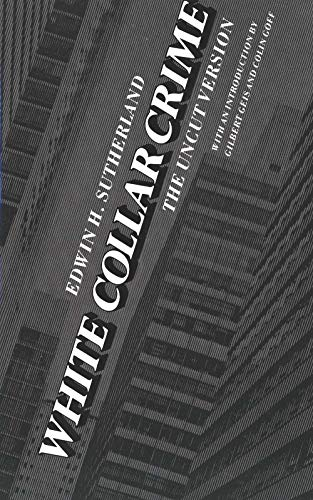
\includegraphics[keepaspectratio]{images/whitecollar.jpg}}\end{minipage}%
%
\begin{minipage}{0.34\linewidth}
\pandocbounded{
\includegraphics[keepaspectratio]{images/corporate.jpg}}\end{minipage}%

\end{figure}%

La criminología hasta la irrupción con fuerza de voces feministas dentro
de la disciplina durante la década de 1970 no prestaba suficiente
atención a la mujer como delincuente, víctima o trabajadora del sistema
penal. Es solo a partir de esa década que empieza a generarse una
\textbf{criminología feminista} orientada a corregir esos sesgos
(Renzetti y Buist 2025). Aún más reciente ha sido el descubrimiento de
que los varones también tienen género y que solo podemos entender el
comportamiento delictivo de los varones entendiendo estas identidades
masculinas de género (Messerschmidt 2018). El creciente reconocimiento
de otras identidades de género y sexuales también ha venido asociado al
desarrollo de una \textbf{criminologia queer} (Buist y Lenning 2022),
interesada en entender las mismas desde una perspectiva criminológica.

\begin{figure}

\begin{minipage}{0.29\linewidth}
\pandocbounded{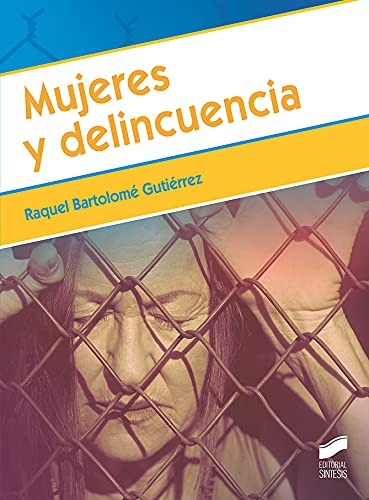
\includegraphics[keepaspectratio]{images/mujeresdelincuencia.jpg}}\end{minipage}%
%
\begin{minipage}{0.26\linewidth}
\pandocbounded{
\includegraphics[keepaspectratio]{images/feminist.png}}\end{minipage}%
%
\begin{minipage}{0.45\linewidth}
\pandocbounded{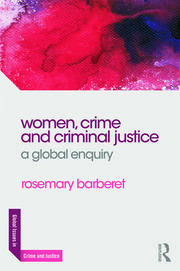
\includegraphics[keepaspectratio]{images/womencrime.jpg}}\end{minipage}%

\end{figure}%

La criminología de caracter biológico del siglo XIX era indudablemente
profundamente racista y contribuyó a través de sus prácticas (Rafter
1997) a legitimar el movimiento eugenésico \footnote{Ver la entrada de
  eugenesia en
  \href{https://es.wikipedia.org/wiki/Eugenesia}{Wikipedia}.} y la
ideología nazi (Rafter 2008).

\begin{quote}
``Al igual que otros miembros de las clases cultas, la mayoría de los
criminólogos del siglo XIX aceptaban los principios del llamado racismo
científico, según el cual los blancos son la raza más evolucionada de
todas. El racismo científico solía formar parte de las explicaciones
evolutivas del comportamiento delictivo: los peores delincuentes son
como salvajes, más cercanos a los hotentotes y otros primitivos de piel
negra que a los blancos normales, con su sentido moral bien
desarrollado.'' (Rafter 2011, 151)
\end{quote}

Varios autores han profundizado en como otros conceptos criminológicos
posteriores, como la subcultura de la violencia propuesta por Marvin
Wolfgang, también contribuían a legitimar estereotipos de caracter
racial durante el siglo XX (Covington 1995). Las últimas décadas han
visto numerosos esfuerzos orientados a identificar los mecanismos por
medio de los cuales el sistema de justicia penal se estructura como
institucionalmente racista.

\pandocbounded{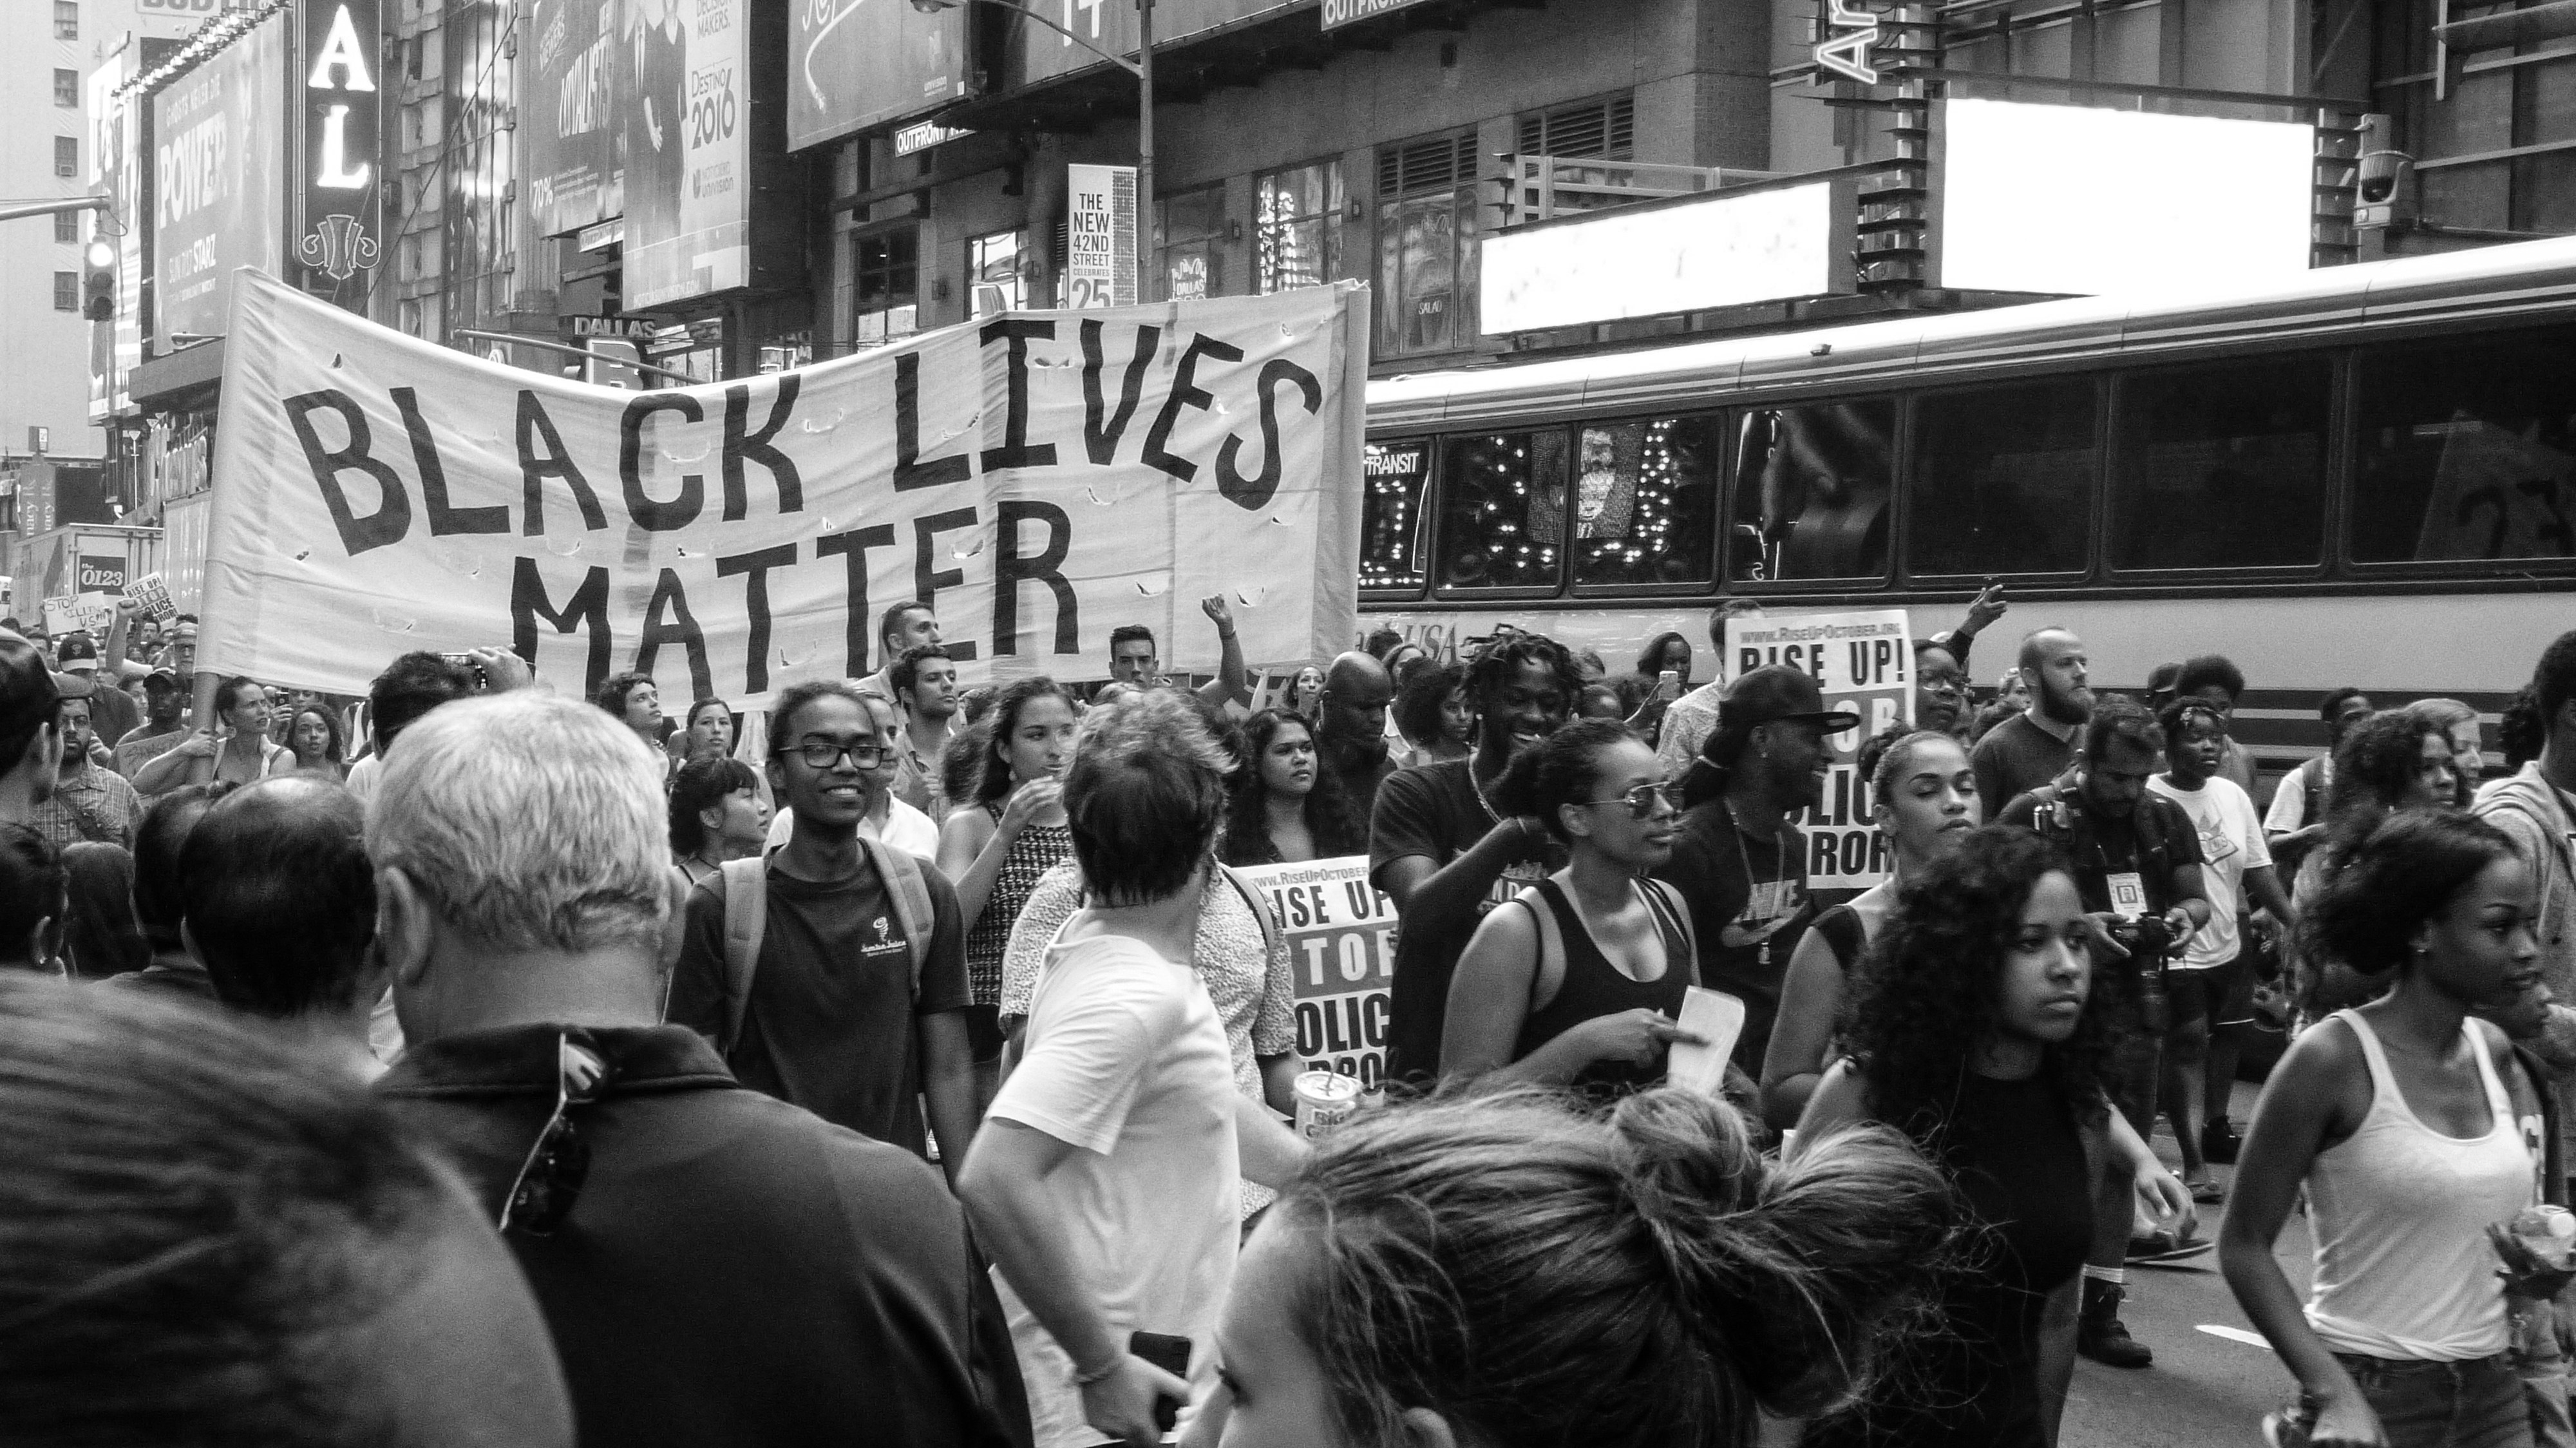
\includegraphics[keepaspectratio]{images/nicole-baster-blacklivesmatter.jpg}}

El desarrollo de la criminología en Estados Unidos y el norte de Europa
han consolidado una serie de teorías y perspectivas que toman como
modelo social el existente en estos países. Son teorías y perspectivas
muchas veces bastante provincianas y asentadas en modos de hacer ciencia
que dan más importancia a todo aquello que tiene lugar en dichas
sociedades (Medina 2011). Se ha tendido a olvidar las experiencias,
vivencias y estructuras existentes en otros países del sur global. De
ahí que en tiempos recientes haya habido voces demandando el desarrollo
de una \textbf{criminología del sur} (Carrington et~al. 2018) que sirva
para el resto del planeta ignorado en el canón criminológico, autores
que defienden perspectivas postcoloniales dentro de nuestra disciplina
(Cunneen 2011), o aquellos que proponen la revelancia de una
criminología más global (Bowling 2011) e interesada en la comparación de
la situación en distintos países (Davi Nelken 2011).

\begin{figure}

\begin{minipage}{0.28\linewidth}
\pandocbounded{
\includegraphics[keepaspectratio]{images/decolonising.jpeg}}\end{minipage}%
%
\begin{minipage}{0.28\linewidth}
\pandocbounded{
\includegraphics[keepaspectratio]{images/southern.webp}}\end{minipage}%
%
\begin{minipage}{0.45\linewidth}
\pandocbounded{
\includegraphics[keepaspectratio]{images/decolonise.jpg}}\end{minipage}%

\end{figure}%

Finalmente, en la sociedad antropocéntrica en la que vivimos estamos
tardando demasiado en entender que vivimos en un planeta finito cuyo
clima y sistemas ecológicos hemos alterado de forma radical en los
últimos doscientos años. Los retos a los que se enfrenta nuestro planeta
como consecuencia de la acción humana en su sistema ecológico son los
más serios a los que se enfrenta la humanidad. La criminología también
puede jugar un papel en entender estos retos. Esta es la visión de
quienes proponen el desarrollo de una
\href{https://www.criminologiaverde.com}{\textbf{criminología verde}}
(South y Brisman 2020).

\begin{figure}

\begin{minipage}{0.31\linewidth}
\pandocbounded{
\includegraphics[keepaspectratio]{images/green.jpg}}\end{minipage}%
%
\begin{minipage}{0.32\linewidth}
\pandocbounded{\includegraphics[keepaspectratio]{images/verde.webp}}\end{minipage}%
%
\begin{minipage}{0.37\linewidth}
\pandocbounded{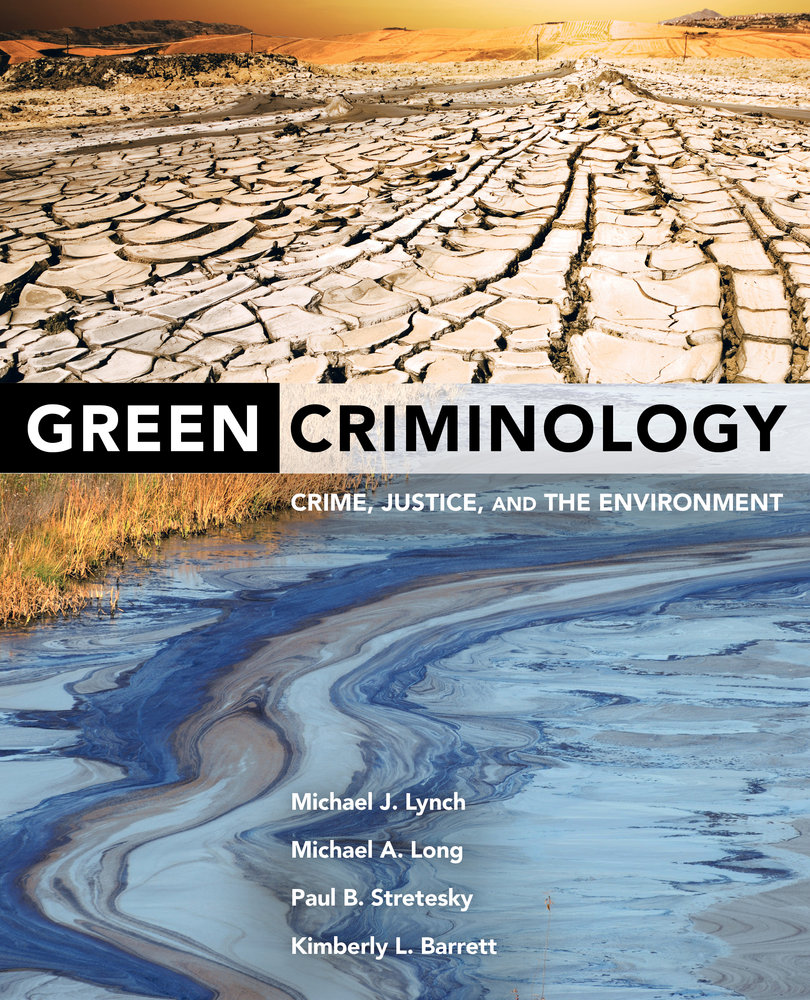
\includegraphics[keepaspectratio]{images/green2.jpg}}\end{minipage}%

\end{figure}%

Estos sesgos en la mirada criminológica a los que aludimos en esta
sección seran estudiados en mayor detalle en la tercera parte de este
volumen, donde dedicaremos un capítulo a cada uno de ellos.

\subsection{Criminología y
política}\label{criminologuxeda-y-poluxedtica}

Una de las cuestiones que ha ocupado a pensadores sociales desde que
aparecen las ciencias sociales es el papel de los valores en el
desarrollo de las mismas. Aunque hay autores que plantean que la
criminología como otras ciencias debe aspirar a la neutralidad política,
hay quienes plantean que la criminología es ineludiblemente política.
Como señala Loader (2022, 65):

\begin{quote}
``La relación entre la criminología y la política es básica, incluso
interna. Desde este punto de vista, la criminología es un campo de
investigación constituido en parte por la política: practicar la
criminología implica, inevitablemente, enfrentarse a cuestiones
políticas. Esto no significa que toda teorización sobre el crimen y la
justicia sea, o tenga que ser, teoría política. Sin embargo, sí
significa que toda investigación teórica y empírica sobre el crimen y su
regulación plantea cuestiones políticas (y tiene implicaciones para las
instituciones políticas) que solo pueden eludirse a costa de comprender
plenamente por qué el delito y las respuestas sociales al delito son
importantes''
\end{quote}

Los procesos de criminalización, la distribucion de recursos sociales
asociados con la delincuencia, las respuestas que damos al
comportamiento delictivo son procesos decididos politicamente y frente a
los que una disciplina que estudia estos procesos no puede permanecer
completamente ``neutral''.

\begin{figure}

\begin{minipage}{0.30\linewidth}
\pandocbounded{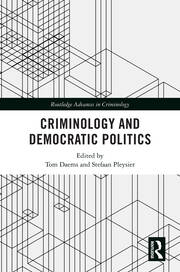
\includegraphics[keepaspectratio]{images/democraticcriminology.jpg}}\end{minipage}%
%
\begin{minipage}{0.31\linewidth}
\pandocbounded{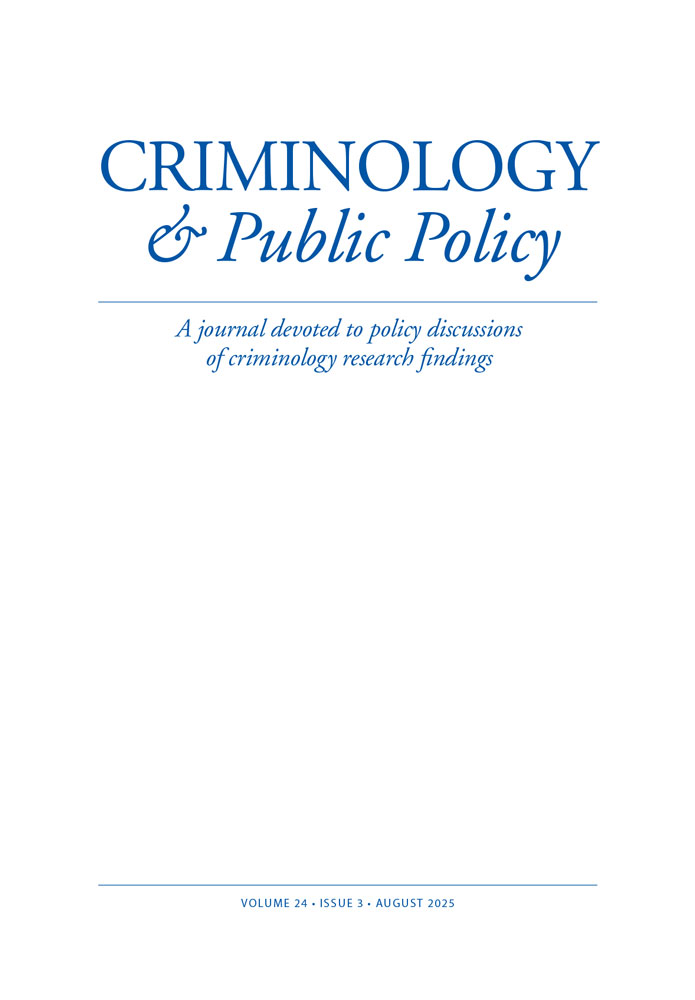
\includegraphics[keepaspectratio]{images/criminologyandpublicpolicy.jpg}}\end{minipage}%
%
\begin{minipage}{0.38\linewidth}
\pandocbounded{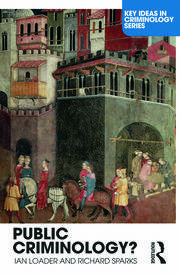
\includegraphics[keepaspectratio]{images/publiccriminology.jpg}}\end{minipage}%

\end{figure}%

Cada teoría criminológica lleva implícita en sí un programa político
criminal, una forma de concebir el delito y una forma de responder al
mismo. Como señala (\textbf{Medina\_25?}), los partidarios de distintas
teorías criminologicas:

\begin{quote}
``pueden tener, explícita o implícitamente, visiones muy diferentes, y a
veces mutuamente excluyentes, sobre la naturaleza humana, el concepto de
una buena sociedad, la prioridad que ha de darse a la seguridad y el
orden en el ámbito político frente a otros valores, el papel del Estado,
la iniciativa privada, y la sociedad en materia de prevención, las
posibilidades de reforma del sistema de justicia penal, la deseabilidad
o posibilidad de cambios sociales más amplios, y otras cuestiones que
tienen una naturaleza o dimensión ideológica (igualdad, libertad,
etc.)''
\end{quote}

En la cuarta parte de este volumen profundizaremos en esta cuestión y
exploraremos las distintas perspectivas que existen en nuestra
disciplina frente a este tipo de cuestiones.

\subsection{Una disciplina plural}\label{una-disciplina-plural}

A lo largo del tiempo la criminología ha ido conformándose como una
disciplina plural. Quienes hacemos investigación criminológica, como ya
hemos apuntado, solemos tener formaciones disciplinarias diversa
(criminología, sociología, psicología, económicas, historia, etc.) que
parcialmente constituyen nuestra identidad, también (como veremos en el
próximo capítulo) tenemos ideas diversas sobre como y hasta que punto se
puede conocer el mundo que nos rodea y cual es son los métodos más
adecuados para estudiar los objetos de la criminología. Igualmente, los
temas que nos interesan dentro de la criminología y las perspectivas
teóricas que mas nos persuaden son diversas entre nosotras, así como la
forma en la que interpretamos la relevancia de los distintos sesgos en
la mirada criminológica a la que he hecho referencia. Es decir, existen
numeros vectores que contribuyen a que haya una multitud de ``tribus''
criminológicas, a menudo asociadas a distintas divisiones o grupos de
trabajo dentro de las principales sociedades científicas de criminología
o pertenecientes a grupos de investigación separados, que se consideran
alternativos a dichas sociedades científicas.

Esta pluralidad, señalado lo que apuntabamos en la sección anterior, a
menudo enmascara diferencias de naturaleza política o ideológica, aunque
no siempre este es el eje determinante. Existe, como en muchos ambitos
de la vida, conflicto. Este conflicto se traduce en diferencias
interpretativas en cuanto a marcos teóricos, lo que podemos considerar
evidencia científica establecida, y las consecuencias político
criminales de dicha evidencia.

Soy de los que piensan que la diversidad y pluralidad de opiniones es
enriquecedora y que hay que mantener una actitud humilde y respetuosa
(esto es dispuesta a la escucha crítica) frente a las opiniones de otros
participantes en la criminología. Desde el punto de vista del alumno o
la alumna que se enfrenta por primera vez a esta cacofonía de voces
puede ser complicado orientarse. Pero esa es precisamente la función y
el trabajo que tenéis por delante en vuestros estudios de criminología.
Entrar en este campo de estudio, mapearlo adecuadamente, y a partir de
ahí ir desarrollando de forma informada vuestra propia posición en el
mismo.

\section{La criminología en
España}\label{la-criminologuxeda-en-espauxf1a}

(Sección en construcción)

\chapter{Método científico y
criminología}\label{muxe9todo-cientuxedfico-y-criminologuxeda}

\section{¿Para qué sirve el
método?}\label{para-quuxe9-sirve-el-muxe9todo}

\section{Dos culturas de
investigación}\label{dos-culturas-de-investigaciuxf3n}

\section{Tipos de investigación}\label{tipos-de-investigaciuxf3n}

\chapter{La delincuencia en España}\label{la-delincuencia-en-espauxf1a}

\section{Las estadísticas
oficiales}\label{las-estaduxedsticas-oficiales}

\section{Las encuestas de
victimización}\label{las-encuestas-de-victimizaciuxf3n}

\section{Los estudios de autoinforme}\label{los-estudios-de-autoinforme}

\section{Nuevas formas de datos}\label{nuevas-formas-de-datos}

\section{¿Es España un país
seguro?}\label{es-espauxf1a-un-pauxeds-seguro}

\part{Temas de estudio}

\chapter{El delito}\label{el-delito}

\section{El delito como objeto de
estudio}\label{el-delito-como-objeto-de-estudio}

\subsection{¿Delito o daño social?}\label{delito-o-dauxf1o-social}

Como hemos visto se suele definir de forma sintética a la criminología
como la ciencia del delito. La propia raíz etimiológica del término
criminología alude a la noción del crimen como central para nuestra
disciplina. Parecería poco controvertido, por tanto, afirmar que el
principal objeto de estudio de la criminología es el delito. Como señala
Gottfredson (2011, 36): ``Limitar la criminología a los comportamientos
que violan la ley penal es sin duda el enfoque más común y sensato de la
criminología.''. Zedner (2011) va aún más lejos, para ella:

\begin{quote}
``La criminología carece de un marco teórico distintivo, una ciencia
diferenciada o una metodología, y debe la cohesión que posee al delito
como su foco de atención y su justificación racional.'' (Zedner 2011,
272)
\end{quote}

Como vamos a ver es algo un poco más complicado. Ya a principios del
siglo XX se produjo un debate entre Edwin Sutherland, considerado una de
los principales criminólogos del siglo XX, y el jurista Paul Tappan
sobre cual era el legítimo ámbito de estudio de la criminología.

Para Tappan (1947) la criminología tenía que centrar su mirada en los
actos definidos como delitos por la legislación penal cuando ya había
una persona acusada y sancionada penalmente por el Estado, mientras que
Sutherland (1949) usaba una definición más sociológica y ampliada a
considerar infracciones legales no necesariamente constitutivas de
ilícitos penales.

El contexto de la discusión fue la introducción del concepto de
\textbf{delincuencia de cuello blanco} propuesta por Sutherland (1949),
y al que retornaremos en capítulos posteriores, pese a que por aquel
tiempo las infracciones que el denominaba como tal no eran infracciones
penales. Confundiendo el estatus legal con la conveniencia científica o
metodológica, Tappan (1947) argumentaba lo siguiente:

\begin{quote}
``Consideramos que el «delincuente de cuello blanco», el infractor de
las normas de conducta y la personalidad antisocial no son delincuentes
en ningún sentido significativo para el científico social, a menos que
haya infringido una ley penal. No podemos considerarlo como tal a menos
que haya sido debidamente condenado. Puede ser un grosero, un pecador,
un leproso moral o el diablo encarnado, pero no se convierte en
delincuente por los insultos sociológicos a menos que la autoridad
política constituida diga que lo es.'' (Tappan 1947, 97)
\end{quote}

No obstante, sería absurdo pretender que la criminología solo estudia o
debería estudiar infracciones penales. Nunca ha sido así, por más que el
estudio del delito sea central a la disciplina, ni probablemente debería
serlo. De hecho algunos autores han sido muy críticos sobre lo que ceder
al Estado y su legislación penal los contornos de nuestra disciplina
implica. En palabras de Colin Sumner (1994, 301-2):

\begin{quote}
``Tomar las categorías políticamente organizadas de dominación estatal y
las categorizaciones de los funcionarios encargados de hacer cumplir la
ley como nociones científicas es convertir las herramientas sectoriales
e históricas del Estado en conceptos de comportamiento universalmente
válidos. Es tomar el Estado como Dios de todo conocimiento y asumir que
incluso el consentimiento popular a la legislación transforma
automáticamente el juicio político vinculado al contexto en verdad
universal. Como tal, es un acto de fe ciega en el orden político
moderno, o el abandono de todos los principios de moralidad e
investigación a los dioses de la carrera profesional, el dinero y el
ascenso. En cualquiera de los dos casos, se trata, en el sentido antiguo
o nuevo de la palabra ideología, de una práctica ideológica.''
\end{quote}

Aunque es cierto que las criminólogas dedican la mayor parte del tiempo
a estudiar infracciones penales, gestionadas por el sistema de justicia
penal, también es cierto que estudian otro tipo de ilícitos o conductas.
Generalmente la focalización en distintos conceptos de lo ``desviado'' o
lo infractor ha venido ligado a distintas perspectivas disciplinarias o
teóricas (dentro de o relacionadas con) la criminología.

Algunos psicólogos que trabajan en el ámbito de la criminología, por
ejemplo, han centrado su atención no en el concepto de delito sino el de
\textbf{desorden de conducta}, un patrón de comportamiento repetitivo y
persistente que puede incluir sustracciones de propiedad, mentiras,
violencia física, vandalismo, incumplimiento imprudente de las normas y
otras formas de comportamiento antisocial. Mientras que durante mucho
tiempo dentro de la sociología hubo un interés notable por la
\textbf{sociología de la desviación}. Esta campo de estudio estaba
interesado en explorar las acciones o comportamientos que violan las
normas sociales de reglas formales, así como las violaciones informales
de las normas sociales (por ejemplo, el rechazo de las costumbres y las
tradiciones). Para estos sociologos el punto de anclaje era la
\emph{desviación}, siendo el delito solo una de las muchas formas de
desviación.

A día de hoy, por ejemplo, hay muchas criminólogas que han desarrollado
buena parte de su carrera estudiando el consumo de drogas (Measham,
Aldridge, y Parker 2001; Measham, Williams, y Aldridge 2011), pese a que
esta no es una conducta delictiva (ni siquiera ilegal) en muchos países.
Lo mismo podríamos decir del ejercicio de la prostitución, aunque en
determinados contextos esta ilegalizada y en algunos países
criminalizada, eso no ocurre en todas las latitudes. No por ello deja de
ser de interés para quienes nos dedicamos a la criminología.

\begin{figure}

\begin{minipage}{0.32\linewidth}
\pandocbounded{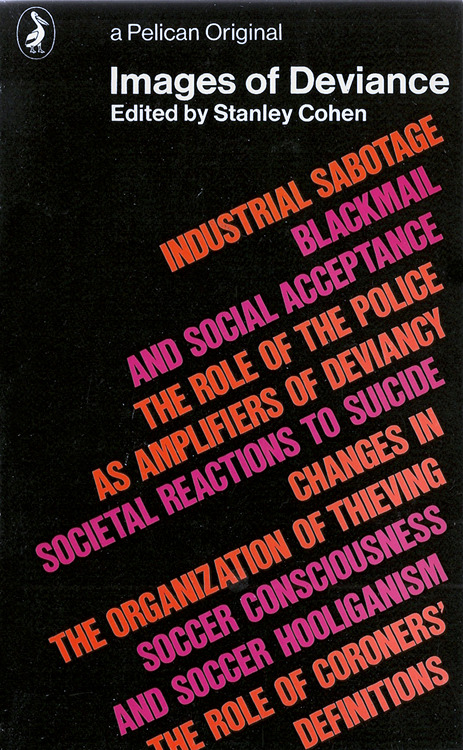
\includegraphics[keepaspectratio]{images/imagesofdeviance.jpg}}\end{minipage}%
%
\begin{minipage}{0.35\linewidth}
\pandocbounded{
\includegraphics[keepaspectratio]{images/waywardpuritans.jpg}}\end{minipage}%
%
\begin{minipage}{0.33\linewidth}
\pandocbounded{
\includegraphics[keepaspectratio]{images/outsiders.jpg}}\end{minipage}%

\end{figure}%

Más recientemente ha habido propuestas de resituar el tema de interés de
nuestra disciplina. Una de estas propuestas es la desarrollada por los
defensores de los llamados \textbf{estudios de la regulación}. Algunos
autores como el criminólogo australiano John Braitwaite, de hecho,
considera vital para la criminología el dedicar mucha más energía de la
dedicada hasta ahora a entender mecanismos reguladores diferente de los
articulados en torno al sistema de control y justicia penal y, por
tanto, prestar más atención, entre otras cosas, al distintos mecanismos
de regulación (y las infracciones ligadas a los mismos).

\begin{quote}
``aunque la disciplina de la criminología está actualmente consolidada
en términos institucionales, las herramientas intelectuales de la
disciplina tienen una relevancia cada vez menor para el mundo social que
está surgiendo\ldots{} las principales tendencias de desarrollo de la
política gubernamental implican un cambio de un estado del bienestar,
gobernado por técnicas keynesianas de gestión de la demanda, a una nueva
forma de estado regulador, basado en una combinación neoliberal de
competencia de mercado, instituciones privatizadas y formas
descentralizadas y a distancia de regulación estatal. Estos nuevos
estilos de gobernanza se basan en el reconocimiento de nuevas fuerzas y
mentalidades sociales, en particular de la lógica globalizadora de la
gestión de riesgos, y reconfigurarán cada vez más los ámbitos social y
político de formas que tendrán consecuencias para la vigilancia y el
control de la delincuencia. El enfoque tradicional de la criminología en
los delitos callejeros y las instituciones policiales, judiciales y
penitenciarias puede ser cada vez menos relevante para los nuevos daños,
riesgos y mecanismos de control que están surgiendo en la actualidad.''
(Braithwaite 2000, 222)
\end{quote}

Vemos así como aspectos importantes de la vida económica y social vienen
a ser regulados por el derecho administrativo que a medida que ha ido
creciendo ha ido aumentando el espacio del derecho administrativo
sancionador y la aparición de entidades reguladoras encargadas de velar
por la aplicación del derecho que no forman parte del sistema de
justicia penal. Retomaremos estas ideas en el capítulo 8, por ahora
valga entender que el estudio de las infracciones administrativas
también puede interesar a la criminología.

\begin{figure}

\begin{minipage}{0.51\linewidth}
\pandocbounded{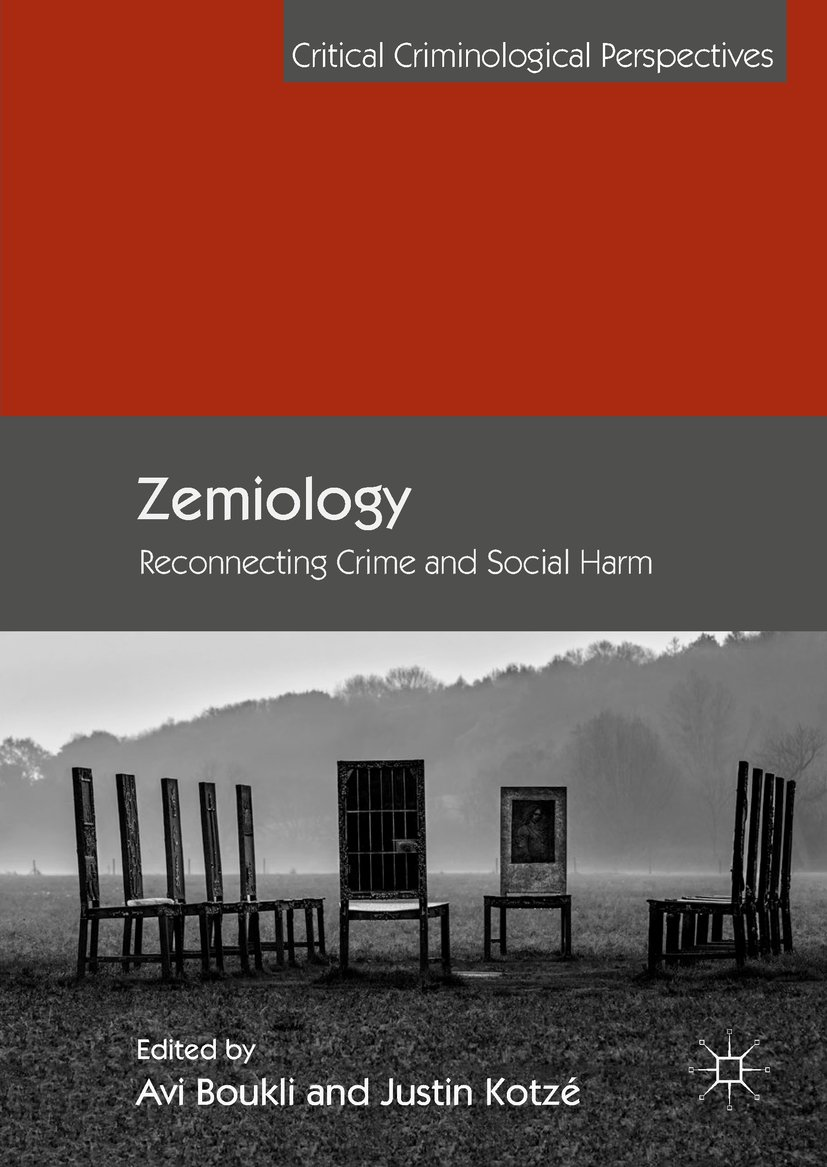
\includegraphics[keepaspectratio]{images/zemiology2.jpg}}\end{minipage}%
%
\begin{minipage}{0.49\linewidth}
\pandocbounded{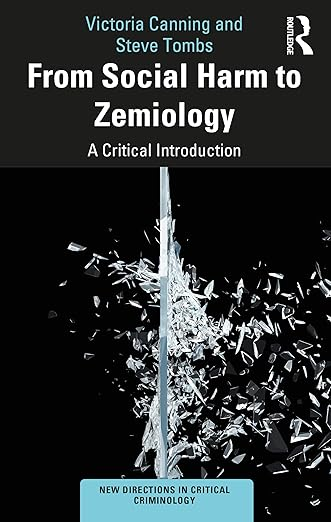
\includegraphics[keepaspectratio]{images/socialharm.jpg}}\end{minipage}%

\end{figure}%

Otros autores han propuesto el desarrollo de una \textbf{zemiología}
como alternativa crítica a la criminología, una disciplina centrada en
el estudio no del delito, sino del \textbf{daño social} (Hillyard y
Tombs 2007). Esta corriente surge para poner el acento en daños sociales
generados por el Estado o grandes corporaciones, pero que rara vez son
criminalizados. Desde esta perspectiva se argumenta que ceñirnos
solamente al estudio de las conductas que son criminalizadas y pasan a
ser, por tanto, tipificadas en las legislaciones penales como delitos
dejaría fuera de nuestra mirada una serie de actos altamente dañosos,
pero que por las dinámicas de poder en la sociedad actual no llegan al
Código Penal. Por el contrario, señalan que pese a las pomposas
declaraciones de penalistas la legislación penal están plagados de
infracciones que recogen comportamientos muy triviales y que
probablemente no merecen reproche penal alguno. Piensan que el control
del delito es ineficaz, doloroso, y perpetuador de diferencias sociales
y que el concepto de delito (y la criminología construida sobre este
concepto) no hace más que legitimar la expansion de este control. Es una
perspectiva que aspira a liberar a las criminólogas del corsé de la
legislación penal. Por tanto proponen que debemos abandonar el estudio
del delito y adoptar, en su lugar, una «perspectiva del daño social» que
no diferencie entre los daños calificados como delitos y otros tipos de
daños.

De tal forma, aunque el delito sigue siendo el principal punto de
anclaje de nuestra disciplina, lo cierto es que probablemente no hay que
ser excesivamente dogmático al respecto. Existen argumentos legítimos
para pensar en otros puntos de anclaje. Pero, por otro lado, tampoco
deberíamos abandonarlo sin más como objeto de estudio. Como bien postula
Zedner (2011, p.) la irrupción de estas perspectivas:

\begin{quote}
``no debe implicar el abandono del delito como categoría jurídica. El
compromiso crítico con el derecho penal y la teoría penal permite
plantear difíciles preguntas sobre la forma en que se llega a las
infracciones delictivas, cómo se definen y estructuran, a quién se
aplican y las consecuencias que deben derivarse de ellas.''
\end{quote}

De hecho, como abordaremos de forma más detallada en el capítulo 8 y
brevemente en la proxima sección, los procesos de criminalizadión:
pensar críticamente sobre la delincuencia, qué justifica la
criminalización, por qué y según qué principios, entra de lleno en el
ámbito de la criminología y merece más atención criminológica de la que
ha recibido hasta ahora (Zedner 2011).

\subsection{¿Pero que es un delito?}\label{pero-que-es-un-delito}

Y esto nos lleva directamente a la siguiente pregunta. ¿Qué es un
delito? Como señala Gottfredson (2011, 35):

\begin{quote}
``A muchos les puede parecer extraño \ldots{} que haya algún problema
para responder a la pregunta «¿qué es el delito?», pero la definición de
delito para la criminología ha sido durante mucho tiempo objeto de un
considerable debate. Sin duda, la respuesta más común se basa en la ley,
es decir, en el comportamiento clasificado como delito en la
legislación. Según esta visión estándar de los libros de texto, un
delito es un comportamiento prohibido por el derecho penal y la tarea de
la criminología es describir y luego explicar los patrones de violación
del derecho penal y los esfuerzos realizados para limitarlos.''
\end{quote}

Los penalistas suelen definir los delitos como las acciones u omisiones
tipificadas como tales por la ley penal que, teóricamente, suponen los
ataques o puestas en peligros más graves de los bienes jurídicos más
importantes para la ciudadanía. Generalmente se considera que un delito
es ``la conducta (acción u omisión) típica, antijuríica, culpable y
punible'' (Muñoz-Conde 2022), que de forma secuencial reune esos
distintos elementos elaborados por la dogmática penal (tipicidad,
antijuridicad, culpabilidad y punibilidad) y que estudiareis en vuestra
asignatura de Derecho Penal.

\begin{quote}
``El derecho penal se ocupa de identificar las formas de comportamiento,
acción u omisión, la estructura de los delitos, los principios jurídicos
subyacentes y los elementos constitutivos que, en ausencia de
justificación o excusa, dan lugar a la responsabilidad penal. Para los
teóricos del derecho penal y los filósofos del derecho, una forma obvia
de resistirse a la criminalización excesiva es desarrollar una
explicación más sólida de lo que debe y no debe ser criminalizado. Se
centran en articular principios y valores para guiar y restringir a
quienes formulan y aprueban nuevas leyes penales, así comoa quienes las
administran.'' (Zedner 2011, 278)
\end{quote}

El delito, no obstante, no solamente es una categoría legal, sino que
también es una construcción social. Las conductas que se consideran
delictivas han ido variando a lo largo del tiempo y los códigos penales
tambian varían de forma significativa entre países. Hay algunas
conductas que suelen ser consideradas delictivas de forma más o menos
universal, pero su regulación y contornos también ha cambiado a lo largo
del tiempo. Cada vez hay un mayor interés por parte de historiadores de
entender el delito y la justicia penal. Estos están produciendo
contribuciones muy relevantes para entender precisamente estas
variaciones a lo largo de la historia.

En todo coso, para hacer frente a esta limitación para ponernos de
acuerdo sobre lo que es un delito, Felson (2006, 35) propone que
adoptemos un enfoque pragmático y consideremos como delito ``cualquier
conducta identificable que un numero apreciable de gobiernos haya
prohibido y a la que aplique sanciones penales''. Otros criminólogos en
cambio proponían una definición del delito que tratase de trascender el
problema de la vinculación a legislaciones penales concretas tratando de
identificar su naturaleza universal (Gottfredson 2011). Así Gottfredson
y Hirschi (1990, 15) definían el delito como ``actos de fuerza o fraude
realizados en beneficio del interés propio''.

El delito también es una construcción social en otro sentido. Como
señala Zedner (2011, 272):

\begin{quote}
``El delito no es solo una cuestión de lo que se define legislativamente
como tal, sino de lo que los funcionarios de la justicia penal realmente
persiguen, investigan, procesan y castigan.''
\end{quote}

En los manuales de justicia penal se hace referencia a menudo a la
metafora del embudo, para aludir a cómo empezamos con los delitos
cometidos, de los que apenas se denuncian la mitad, se resuelve un
porcentaje menor, y muchos menos se adjudican o resuelven a traves del
proceso y castigo penal. Entre el universo legal de delitos contemplados
en el Código Penal y los delitos actualmente denunciados, perseguidos y
penalmente resueltos media (y siempre mediará) un amplio abismo.

Como señalan Felson y Eckert (2019):

\begin{quote}
``En la mayoría de los delitos conocidos por la policía, nadie es
arrestado. Cuando hay un arresto, la mayoría de los casos nunca se
envían al fiscal. De los casos que llegan a juicio, la mayoría conducen
a un acuerdo entre el abogado y el fiscal, no a un juicio. De los que
llegan a juicio, es mucho más probable que se celebre un juicio sin
jurado en un tribunal \ldots{} local que un juicio con jurado en toda
regla, como se ve en la televisión. Incluso las personas condenadas
tienen muchas posibilidades de evitar el encarcelamiento, a pesar de
varias décadas de políticas de «ley y orden». Por ejemplo, se estimaron
unos 3,3 millones de robos en viviendas en Estados Unidos en 2016.11 De
ellos, aproximadamente la mitad de los incidentes se denunciaron a la
policía. Aproximadamente 1 de cada 10 resultó en arrestos. Estimamos que
solo alrededor del 1 por ciento de los robos dan lugar a una condena y
aún menos a encarcelamiento. La probabilidad de ser castigado por un
delito relacionado con las drogas es aún mucho menor.''
\end{quote}

\begin{figure}[H]

{\centering \pandocbounded{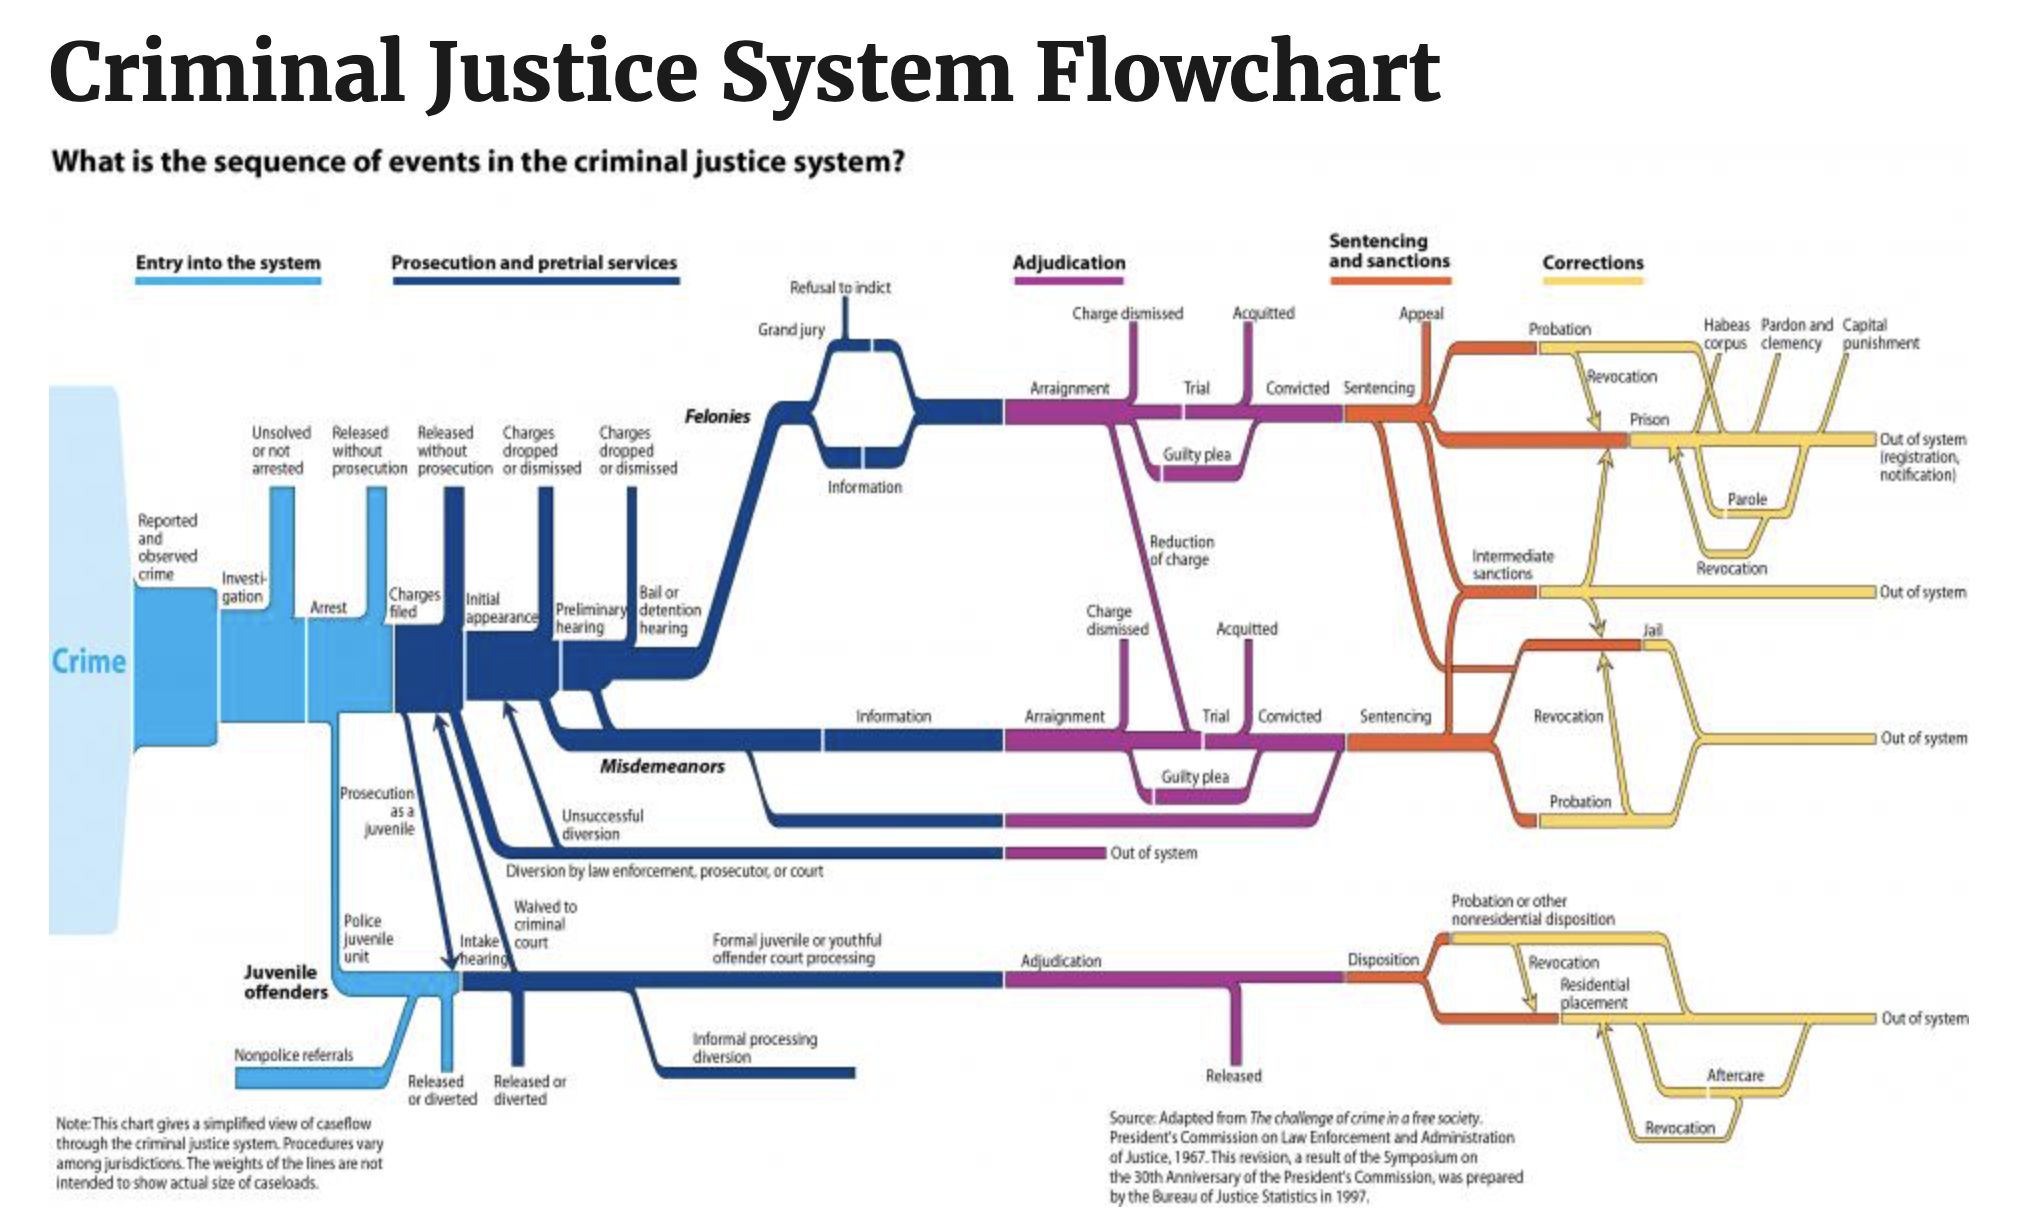
\includegraphics[keepaspectratio]{images/flowchart.png}}

}

\caption{Diagrama de flujo del sistema de justicia penal (Fuente: US
Bureau of Justice Statistics)}

\end{figure}%

De lo que se deriva que (Zedner 2011, 279-80):

\begin{quote}
``Comprender cómo se construye el delito en los medios de comunicación,
la política y la opinión pública, en la labor policial y en el proceso
de justicia penal sea un antídoto importante contra el enfoque de la
«ley en los libros», cuyo enfoque tradicional se centra en el derecho
doctrinal\ldots{} Sin prestar atención a los procesos políticos y
sociales por los que se construye y media la delincuencia; los
impulsores y limitaciones administrativos, financieros y políticos del
enjuiciamiento y el castigo; y los contextos sociales, culturales y
profesionales en los que actúan los agentes de la justicia penal, existe
el peligro de que se dé una visión en gran medida artificial de la
delincuencia\ldots{} Una función fundamental de la criminología es
aportar pruebas de cómo se produce la criminalización, no solo en las
páginas de los códigos penales y los informes jurídicos, sino también en
las complejas interacciones entre los medios de comunicación, los
políticos y la opinión pública; en la toma de decisiones y el ejercicio
de la discrecionalidad por parte de los funcionarios de la justicia
penal; y a lo largo de esa entidad tortuosa que es el proceso penal. La
criminología también tiene mucho que decir sobre las relaciones de
poder, sobre todo las de clase, raza y género, que subyacen a la
decisión de criminalizar e informar las prácticas policiales y
punitivas. Revela los factores contingentes, los supuestos y prejuicios
culturales y los imperativos políticos que sustentan la decisión de
considerar criminal un acto u omisión.''
\end{quote}

La criminología se preocupa, por tanto, por al menos tres tipos de
cuestiones en lo que refiere al delito:

\begin{itemize}
\item
  ¿Cómo determinados actos u omisiones vienen a ser definidos como
  delitos y cuáles son los procesos, intereses y dinámicas que guían los
  actos legislativos de criminalización y de descriminalización?
\item
  ¿De qué forma las instancias del sistema de justicia penal (policía,
  fiscales, jueces, prisiones) actúan frente al delito en la práctica y
  cuales son los factores que condicionan e influyen estas respuestas?
\item
  ¿Que delitos se cometen y cuándo, donde, cómo y por qué (con
  independencia de la respuesta que las instancias del Estado den a
  estos delitos)?
\end{itemize}

Las dos primeras preguntas serán abordades de forma más detenida en el
capítulo 8. En el apartado 2 de esta capítulos nos centraremos en la
tercera de ellas. Pero antes nos vamos a adentrar brevemente en otro
debate: ¿Existen rasgos más o generales que definan a los actos que
definimos como delictivos?

\subsection{¿Las características generales del
delito?}\label{las-caracteruxedsticas-generales-del-delito}

Si nos dejaramos llevar por los medios de comunicación social,
tendriamos que caracterizar los delitos como eventos dramáticos y
generalmente violentos. Tanto la industria del entretenimiento como los
medios informativos compiten en la economía de la atención y buscan
captar la nuestra contando historias sobre delitos que reunen estas
características. (\textbf{Felson?}) llama esto la \emph{falacia del
drama}:

\begin{quote}
``La mayoría de los actos delictivos no son muy inteligentes ni
románticos. La falacia dramática afirma que los delitos más publicitados
están muy alejados de la vida real. Los medios de comunicación se dejan
llevar por una secuencia de horror y distorsión. Encuentran una historia
de terror y luego entretienen al público con ella. Ganan dinero con
ello, al tiempo que crean un mito en la mente del público. Luego se
basan en ese mito para la siguiente historia de terror. Así, el crimen
se vuelve muy distorsionado en la mente del público''
\end{quote}

Marcus Felson es uno de los autores que precisamente más ha insistido en
la necesidad de desarrollar una visión más realista y prosaica del
delito. Su obra está llena de perlas que le sirven para subrayar esto:

\begin{quote}
``Los detectives ficticios de televisión no tendrían ningún interés en
la mayoría de \ldots{} asesinatos''
\end{quote}

\begin{quote}
``La mayoría de los asesinatos son el trágico resultado de una pequeña y
estúpida disputa. De hecho, el asesinato es menos un delito que una
consecuencia. El camino hacia el asesinato no difiere mucho del de una
pelea común, salvo que, por desgracia, alguien ha muerto. El asesinato
tiene dos características fundamentales: una pistola demasiado cerca y
un hospital demasiado lejos''
\end{quote}

\begin{quote}
``El trabajo policial consiste en horas y horas de aburrimiento\ldots{}
El riesgo anual de morir en acto de servicio es solo del 0,000113, es
decir, aproximadamente 11 por cada 100 000 agentes''
\end{quote}

\begin{quote}
``La mayoría de los delitos son muy sencillos y no requieren habilidades
avanzadas''
\end{quote}

\begin{quote}
``La mayoría de las organizaciones criminales son muy rudimentarias''
\end{quote}

\begin{quote}
``Las bandas delictivas son extremadamente aburridas la mayor parte del
tiempo''
\end{quote}

Aunque estamos acostumbrados a una determinada imagen del delito, esta
está contaminada por las narraciones que del mismo se hacen en los
medios de comunicación que tienden a exagerar la prevalencia de
determinados delitos y una serie de características de los mismos que
generalmente no están presentes en la mayor parte de las transgresiones
que se producen en la vida cotidiana.

En 1990 Michael Gottfredson y Travis Hirschi publicaron un libro,
\emph{A general theory of crime}, que ha sido muy influyente en nuestra
disciplina. En este libro ellos proponían una nueva teoría del delito
que tendréis ocasión de estudiar en vuestras asignaturas de teoría del
delito (la teoría del autocontrol). En el capítulo segundo de este
libro, Gottfredson y Hirschi (1990, 16) proponían tratar de identificar
los rasgos esenciales del delito. Para estos autores:

\begin{quote}
``El hecho es que la gran mayoría de los actos delictivos son asuntos
triviales y mundanos que provocan pocas pérdidas y menos ganancias. Se
trata de sucesos cuya distribución temporal y espacial es muy
predecible, que requieren poca preparación, dejan pocas consecuencias
duraderas y, a menudo, no producen el resultado deseado por el
delincuente.''
\end{quote}

Gottfredson y Hirschi (1990) consideran que lo que sabemos sobre la
distribución espacio temporal del delito sugiere que los delincuentes
muestran una reticencia a esforzarse en la comisión de delitos;
demuestran que la accesibilidad aumenta el riesgo de las víctimas
potenciales; y muestran que evitar ser detectado forma parte del cálculo
del delincuente. Los delitos comunes, que son la gran mayoría de los
delitos, requieren poco esfuerzo, planificación, preparación o habilidad
y tienen un coste para las víctimas que es generalmente muy trivial en
términos económicos o personales. Si casi la mitad de los delitos no se
denuncian es precisamente porque las víctimas no los consideraron
suficientemente importantes como para tomarse la molestia, como las
encuestas de victimación nos recuerdan una y otra vez.

Evidentemente es muy dificil hacer generalizaciones y siempre hay
excepciones, por raras que sean. Pero si algo debéis derivar de las
observaciones de (\textbf{Feson\_19?}) y Gottfredson y Hirschi (1990) es
que es importante aproximarse al estudio del delito con una visión mucho
más prosaica del mismo de la que hemos adquirido a traves de los medios
de comunicación social.

\section{El delito como evento espacio
temporal}\label{el-delito-como-evento-espacio-temporal}

\subsection{La estadística moral}\label{la-estaduxedstica-moral}

El análisis de las variaciones temporales y espaciales, el dónde y el
cuándo, de la delincuencia han jugado un papel central en la práctica de
la criminología científica. La llamada escuela de la \textbf{estadística
moral} inauguró este tipo de estudios y aproximaciones empíricas al
delito.

Autores como el francés André-Michel Guerry y el belga Adolphe Quetelet,
durante el siglo XIX, realizaron contribuciones fundamentales al estudio
científico de la delincuencia al introducir métodos estadísticos y
análisis empíricos para comprender los patrones delictivos. Su trabajo
sentó las bases de la criminología y las ciencias sociales modernas al
demostrar que la delincuencia podía estudiarse de forma sistemática
utilizando datos y razonamientos estadísticos.

\begin{figure}[H]

{\centering \pandocbounded{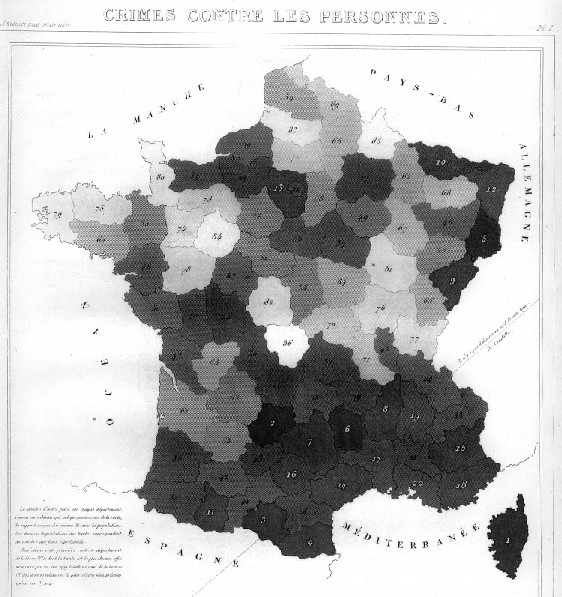
\includegraphics[keepaspectratio]{images/AMGuerry-carte1-low.jpg}}

}

\caption{Mapas del delito en Francia producidos por Guerry}

\end{figure}%

El \emph{Essai sur la Statistique Morale de la France} (Ensayo sobre la
estadística moral de Francia) de Guerry, publicado en 1833, y los
estudios estadísticos de Quetelet en Bélgica utilizaron tablas y mapas
temáticos para relacionar las tasas de criminalidad con variables
sociales como la alfabetización, la riqueza y la geografía.

Sus análisis revelaron que las tasas de criminalidad no eran aleatorias,
sino que mostraban patrones consistentes en todas las regiones y épocas,
lo que sugiere que los factores sociales, y no solo las decisiones
individuales, influían en el comportamiento delictivo. Contrariamente a
la creencia popular, descubrieron que las tasas de criminalidad solían
ser más altas en las zonas más ricas, lo que atribuyeron a las mayores
oportunidades para delinquir, más que a la pobreza por sí sola.

Las primeras investigaciones de Quetelet demostraron que muchos tipos de
delitos siguen patrones estacionales, y que ciertos delitos alcanzan su
punto álgido en épocas específicas del año. Por ejemplo, los delitos
violentos suelen aumentar durante los meses más cálidos, un patrón que
se ha confirmado y ampliado en investigaciones posteriores. Su trabajo
demostró que estas regularidades temporales se mantenían estables a lo
largo de los años, lo que sugiere que la delincuencia está influenciada
por factores sociales y ambientales recurrentes, en lugar de ser
puramente aleatoria o deberse únicamente a decisiones individuales.

El enfoque empírico y basado en datos de Guerry y Quetelet sentó las
bases para desarrollos posteriores en criminología, incluyendo el
análisis espacial, los estudios ecológicos y el uso de métodos
cuantitativos en las ciencias sociales.

\subsection{La criminología ambiental y la geografía del
delito}\label{la-criminologuxeda-ambiental-y-la-geografuxeda-del-delito}

La criminología siguió trabajando el estudio de la geofrafía del delito,
con un grado creciente de sofisticación estadística y metodológica
(Medina y Solymosi 2023) hasta nuestros días. Hoy esta es una de las
áreas de mayor actividad investigadora en la criminología.

La \emph{American Society of Criminology} tiene una división dedicada al
estudio de variaciones espaciales (\emph{Community and Place}), la
\emph{European Society of Criminology} tiene un grupo de trabajo en
criminologia espacial (\emph{Space, place, and crime}) y la
\emph{Sociedad Española de Investigación Criminológica} no se queda
atrás, con un grupo en criminología ambiental. Algunos grados de
criminología en España ya incorporan asignaturas optativas en
herramientas cartográficas (sistemas de información geográfica) para
aprender a hacer mapas del delito y análisis espaciales. Finalmente,
muchos departamentos de policía en otros países (en España aún es
inusual) emplean a criminólogas o geografos para hacer este tipo de
trabajo como \textbf{analistas del delito} y producir informes que
sirvan para el desarrollo de respuestas estratégicas y tácticas. La
criminología espacial o ambiental ha experimentado un crecimiento
notable, por tanto, también a nivel institucional.

La criminología ambiental ha venido a documentar que el delito no se
distribuye de forma aleatoria, sino que determinadas regiones, ciudades,
barrios, calles, y lugares concentran un volumen desproporcionado de
delitos. Estos lugares con altos niveles de delincuencia es lo que se
llaman \emph{puntos calientes} (hot spots en inglés). Este hecho es tan
universal y bien documentado que algunos criminólogos consideran que
podemor hablar de la existencia de una \emph{ley de la concentración}
espacial (Weisburd 2015).

Históricamente ha habido un desplazamiento en el foco de interes. Cuando
Guerry desarrollaba sus mapas de la delincuencia en Francia en el siglo
XIX estaba estudiando variación regional; la llamada \emph{Escuela de
Chicago} (que estudiaréis en la asignatura de teorías criminológicas)
estaba interesada en entender diferencias entre barrios; estudios más
recientes, por el contrario, estan interesados en entender que calles,
que intersecciones de calles, o que direcciones concretas o lugares
concentran más delincuencia. Hemos pasado de estudiar variación a nivel
más agregado a unidades de análisis más localizadas.

La criminología espacial ha estado interesada en entender cuestiones
diversas como, por ejemplo (Bruinsman y Johnson 2018; Andresen 2019):

\begin{itemize}
\item
  ¿Cuáles son los factores que explican la concentración del delito en
  distintos espacios?
\item
  ¿En qué medida es relevante la movilidad humana en los espacios
  urbanos para entender la distribución territorial del delito?
\item
  ¿De que forma los delincuentes y las víctimas se desplazan en el
  espacio y en qué medida es esto relevante?
\item
  ¿Que características del espacio físico/arquitectonico y del diseño
  urbano contribuyen al delito?
\item
  ¿Existen algunos usos del espacio público que pueden ser criminógenos?
\item
  ¿Es posible predecir que zonas tendrán niveles elevados del delito en
  el futuro?
\item
  ¿Podemos identificar la probable residencia de delincuentes en serie
  si conocemos donde han cometido sus delitos?
\item
  ¿Es el delito contagioso a nivel espacial?
\item
  ¿Cual es la mejor forma de construir y diseñar vivienda de protección
  oficial para inhibir la delincuencia?
\item
  ¿Que pueden hacer los \emph{gestores del espacio} (Eck, Linning, y
  Herold 2023) para prevenir el delito?
\item
  ¿Que impacto tiene el delito en las comunidades y espacios en los que
  ocurre?
\end{itemize}

{[}TERMINAR CITANDO EL ARTICULO EN PAPERS 67 E INSERTAR ALGUNOS MAPAS DE
VIPOLIS{]}

\subsection{El análisis temporal del
delito}\label{el-anuxe1lisis-temporal-del-delito}

Las variaciones temporales en la delincuencia también son un importante
objeto de estudio para la criminología. Las investigaciones modernas
concluyen sistemáticamente que las tasas de delincuencia fluctúan a lo
largo del tiempo, mostrando tanto ciclos estacionales predecibles como
patrones temporales más complejos a escala diaria, semanal y mensual.
Sin embargo, la intensidad, el momento y las causas de estas variaciones
difieren según el tipo de delito, el clima y el contexto local.

\begin{tcolorbox}[enhanced jigsaw, bottomtitle=1mm, toprule=.15mm, colbacktitle=quarto-callout-note-color!10!white, bottomrule=.15mm, leftrule=.75mm, colframe=quarto-callout-note-color-frame, opacitybacktitle=0.6, titlerule=0mm, breakable, colback=white, left=2mm, arc=.35mm, title=\textcolor{quarto-callout-note-color}{\faInfo}\hspace{0.5em}{Nota}, toptitle=1mm, coltitle=black, rightrule=.15mm, opacityback=0]

\textbf{Las tendencias históricas del delito}

Hay un creciente interés por entender cambios en la delincuencia a largo
plazo. Por las dificultades de obteber datos fiables sobre otras formas
de delincuencia, buena parte de la investigación se ha centrado en
estudiar los patrones de la violencia, fundamentalmente en Europa, desde
mediados del siglo XVI hasta nuestros días. El trabajo de Eisner (2003)
en este ámbito es de obligada lectura. Eisner (2003, 83) observa que:

``se pueden distinguir diferentes trayectorias a largo plazo en la
disminución de los homicidios entre las distintas regiones europeas. Sin
embargo, los patrones de edad y sexo en los delitos violentos graves han
cambiado muy poco a lo largo de varios siglos. La disminución a largo
plazo de las tasas de homicidios parece ir acompañada de una disminución
desproporcionada de los homicidios entre las élites y de una caída de
los conflictos entre hombres en el espacio público. Se han ofrecido
diversas explicaciones teóricas para esta disminución a largo plazo,
entre ellas los efectos del proceso de civilización, el fortalecimiento
de los poderes del Estado, la Reforma protestante y el individualismo
moderno, pero la mayoría de las teorías han sido post hoc.''

Otros autores han invitado a la cautela en relación con estas
interpretaciones. Aebi y Linde (2016, 57) señalan que:

``explicar la disminución de la violencia interpersonal en los países
industrializados occidentales desde finales de la Edad Media mediante el
efecto de un proceso civilizador requiere pasar por alto los genocidios,
las matanzas masivas y los crímenes de guerra cometidos en estos países
y en sus antiguas colonias.''

Mientras que Schwerhoff et~al. (2021, 1) sugieren que:

``un análisis crítico exhaustivo de las fuentes plantea serias dudas
sobre la solidez empírica de la tesis del declive. Las formas y los
contenidos de las fuentes son inmensamente heterogéneos y un examen más
detallado de la supuesta riqueza de los datos revela lagunas notables.
Además, las estimaciones de población medievales y de principios de la
Edad Moderna son muy poco fiables. Por lo tanto, defendemos que la
investigación histórica sobre la violencia debe volver a centrarse en
constelaciones históricas específicas, aceptar la necesidad de un
análisis crítico minucioso de las fuentes y prestar especial atención a
los contextos de la violencia.''

\end{tcolorbox}

Los delitos se encuentran altamente concentrados en momentos específicos
del día y de la semana, pero la intensidad de estas concentraciones
varía por tipo de delito y región. Por ejemplo, algunos estudios
sugieren que los robos a usarios de bancos o servicios de entrega de
comida a domicilio suelen concentrarse en horas muy concretas, mientras
que los hurtos y otro tipo de robos exhiben una menor concentración
(Prieto-Curiel 2021). Estos ``puntos calientes'' temporales son estables
en el tiempo y pueden ser visualizados como ``latidos'' (heartbeats) del
delito, mostrando periodos de alto y bajo riesgo.

\begin{figure}[H]

{\centering \pandocbounded{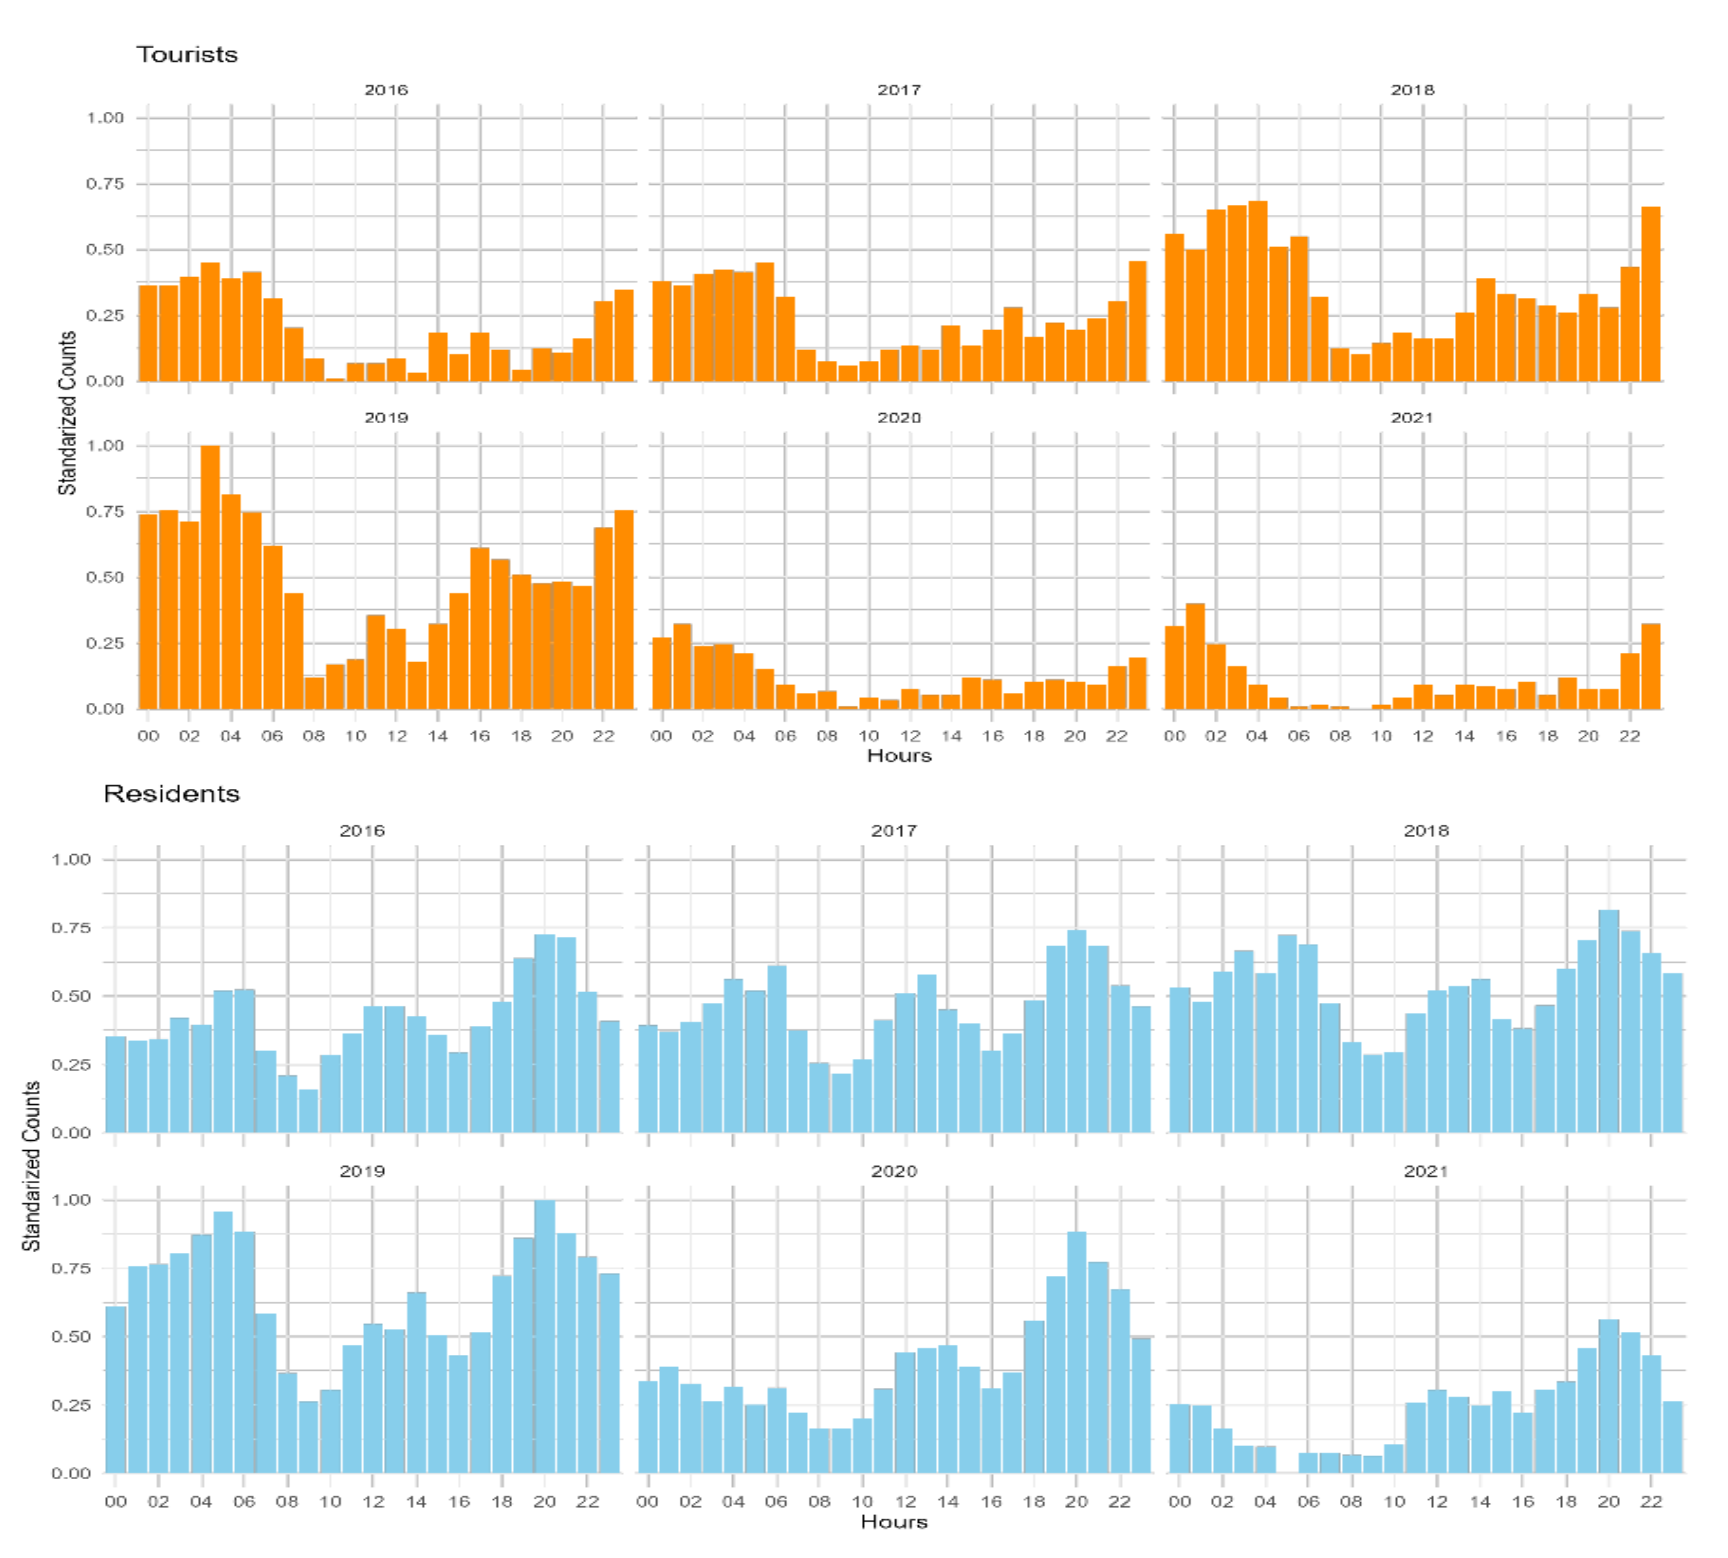
\includegraphics[keepaspectratio]{images/hours.png}}

}

\caption{Tasas estandarizadas de delitos de robos en Barcelona por hora
y año para turistas y residentes.En ambos casos, los robos se concentran
a última hora de la tarde, a última hora de la noche y a primera hora de
la mañana. Pero los residentes muestran un patrón distintivo en forma de
«W» con un aumento pronunciado durante las primeras horas de la tarde,
desde el mediodía hasta las 14:00. Fuente: Trinidad, Medina y Marteache,
2024}

\end{figure}%

Los delitos suelen aumentar los fines de semana y durante la noche,
especialmente para las lesiones y ciertos robos en zonas nocturnas de
ocio y entretenimiento, para luego descender dramáticamente durante la
madrugada. En los puntos de conexión de los sistemas de transporte
público, los delitos son mas comunes durante las noches, y en los
períodos vacacionales, con factores ambientales (por ejemplo, la
presencia de establecimientos de venta de alcohol) influenciando estos
patrones.

La mayoría de los estudios indican que los delitos violentos y contra la
propiedad tienden a alcanzar su punto álgido en verano y a disminuir en
invierno, pero abundan las excepciones y los matices, ya que algunos
delitos muestran poca o ninguna estacionalidad y los patrones espaciales
suelen permanecer estables incluso cuando las tasas generales fluctúan.
Entre las explicaciones de estos patrones se encuentran \textbf{la
teoría de la actividad rutinaria}, los efectos meteorológicos y los
factores sociales y ambientales, pero la interacción entre estos
factores es compleja y, en ocasiones, controvertida (Andresen y Malleson
2013; McDowall, Loftin, y Pate 2011; Linning, Andresen, y Brantingham
2016). Los recientes avances en el análisis de datos y la modelización
espacio-temporal han profundizado nuestra comprensión, revelando tanto
la previsibilidad como la variabilidad de los ciclos delictivos en
diferentes entornos.

{[}INSERTAR FIGURA{]}

\begin{tcolorbox}[enhanced jigsaw, bottomtitle=1mm, toprule=.15mm, colbacktitle=quarto-callout-note-color!10!white, bottomrule=.15mm, leftrule=.75mm, colframe=quarto-callout-note-color-frame, opacitybacktitle=0.6, titlerule=0mm, breakable, colback=white, left=2mm, arc=.35mm, title=\textcolor{quarto-callout-note-color}{\faInfo}\hspace{0.5em}{Nota}, toptitle=1mm, coltitle=black, rightrule=.15mm, opacityback=0]

\textbf{La teoría de las actividades rutinarias}

La teoría de las actividades rutinarias fue desarrollada precisamente
para tratar de entender cambios en los niveles de delincuencia.
Inicialmente desarrollada por Marcus Felson y Lawrence E. Cohen en un
artículo titulado \emph{Social change and crime rate trends: a routine
activity approach}, esta teoría ofrece una perspectiva única sobre las
tendencias de las tasas de criminalidad al enfocarse en las
circunstancias en las que ocurren los actos delictivos predatorios, en
lugar de las características o motivaciones de los delincuentes. La
teoría argumenta que el delito no es simplemente el resultado de
inclinaciones criminales individuales, sino que está fundamentalmente
moldeado por las oportunidades que se presentan a través de las
actividades rutinarias de la vida diaria.

L. Cohen y Felson (1979) consideran que ara que un delito ocurra se
tiene que producir la convergencia espacio temporal de tres elementos:

\begin{itemize}
\item
  \emph{Un delincuente potencial}: La teoría da por sentada la
  existencia de individuos con inclinaciones criminales, sin profundizar
  en las razones específicas de su motivación.
\item
  \emph{Un objetivo adecuado}: Esto se refiere a una persona u objeto
  que sea atractivo como objetivo para un delincuente. La idoneidad de
  un objetivo está influenciada por cuatro elementos clave, a menudo
  resumidos por el acrónimo VIVA:

  \begin{itemize}
  \item
    Valor: Cuán deseable es el objetivo para el delincuente (por
    ejemplo, CDs populares sobre los clásicos).
  \item
    Inercia: La facilidad con la que el objetivo puede ser movido o
    transportado (por ejemplo, los productos electrónicos ligeros son
    más susceptibles que los electrodomésticos pesados).
  \item
    Visibilidad: Cuán expuesto está el objetivo a posibles delincuentes
    (por ejemplo, mostrar dinero en público o dejar objetos de valor
    cerca de una ventana).
  \item
    Acceso: Cuán fácilmente puede un delincuente llegar al objetivo (por
    ejemplo, patrones de calles, bienes colocados cerca de una puerta).
  \end{itemize}
\item
  \emph{La ausencia de un guardián capaz}: Un guardián es cualquiera
  cuya presencia o proximidad podría disuadir un crimen. Este es a
  menudo un ciudadano común ---como un ama de casa, un hermano, un amigo
  o un transeúnte--- en lugar de un oficial de policía o un guardia de
  seguridad, y su vigilancia puede ser inadvertida. Cuando los
  guardianes están ausentes, el objetivo se vuelve particularmente
  vulnerable al ataque.
\end{itemize}

La teoría de la actividad rutinaria argumenta que la oportunidad es una
``causa fundamental'' del delito, mas importante como las variables
personales y sociales. Sostiene que los cambios en la vida comunitaria y
la estructura social pueden aumentar las tasas de criminalidad
simplemente al alterar la cantidad de oportunidades delictivas, incluso
sin ningún cambio en las motivaciones de los posibles delincuentes. La
teoría establece explícitamente que ningún crimen puede ocurrir sin las
oportunidades físicas para llevarlo a cabo; por lo tanto, las
oportunidades de crimen son condiciones necesarias para que el crimen
ocurra.

La teoría destaca cómo la organización espacial y temporal de las
actividades sociales facilita o dificulta que las personas traduzcan las
inclinaciones criminales en acción. Una hipótesis central es que la
dispersión de actividades fuera de los hogares y las familias aumenta
las oportunidades delictivas y, por lo tanto, conduce a tasas de
criminalidad más altas. Por ejemplo, el aumento de mujeres que
ingresaron a la fuerza laboral remunerada a tiempo completo significó
que más hogares quedaran sin vigilancia durante el día, contribuyendo a
un aumento de los robos en domicilios.

Igualmente, los cambios sociales a gran escala, como los avances
tecnológicos y los cambios en la organización social, influyen
significativamente en las oportunidades delictivas. La difusión de
ordenadores portatiles y otros dispositivos moviles de alto valor llevó
a un aumento en el volumen de bienes duraderos ligeros y fácilmente
robables. El mayor uso de automóviles expandió el territorio accesible a
los delincuentes depredadores y dejó más coches vulnerables al robo.

Para estos autores es fundamental entender que las oportunidades del
delito no se distribuyen de manera uniforme, sino que se concentran en
tiempos y lugares específicos, reflejando los ritmos diarios y los
movimientos de personas y propiedades. En ese sentido, las actividades
ilegales se ``alimentan de'' y son ``interdependientes con'' las
actividades rutinarias y legales de la vida cotidiana. Los mismos
factores que aumentan las oportunidades para actividades legítimas (como
la libertad de movimiento, nuevos bienes de consumo, vida social) pueden
también aumentar inadvertidamente las oportunidades para el crimen
predatorio.

\end{tcolorbox}

La delincuencia aumenta cuando hay más gente en la calle o durante las
vacaciones. El clima y la temperatura pueden influir en la delincuencia,
pero sus efectos suelen ser secundarios con respecto a los factores
sociales y relacionados con cambios en las actividades cotidianas de las
personas, y la variabilidad interanual puede ser elevada. Algunos
estudios advierten contra la atribución excesiva de la estacionalidad al
clima, señalando la importancia de los factores estocásticos y sociales.

{[}INSERTAT FIGURA{]}

El mes del año es un fuerte indicador de los niveles de delincuencia en
muchos contextos, lo que respalda el uso de la estacionalidad en la
previsión de la delincuencia y la asignación de recursos. Sin embargo,
existen excepciones: algunos delitos (por ejemplo, los homicidios)
muestran una estacionalidad débil o inconsistente, y los patrones
microespaciales pueden permanecer estables incluso cuando las tasas
generales fluctúan. La pandemia de COVID-19 (Nivette et~al. 2021) y
otras perturbaciones sociales importantes pueden anular los patrones
estacionales típicos.

\begin{figure}[H]

{\centering \pandocbounded{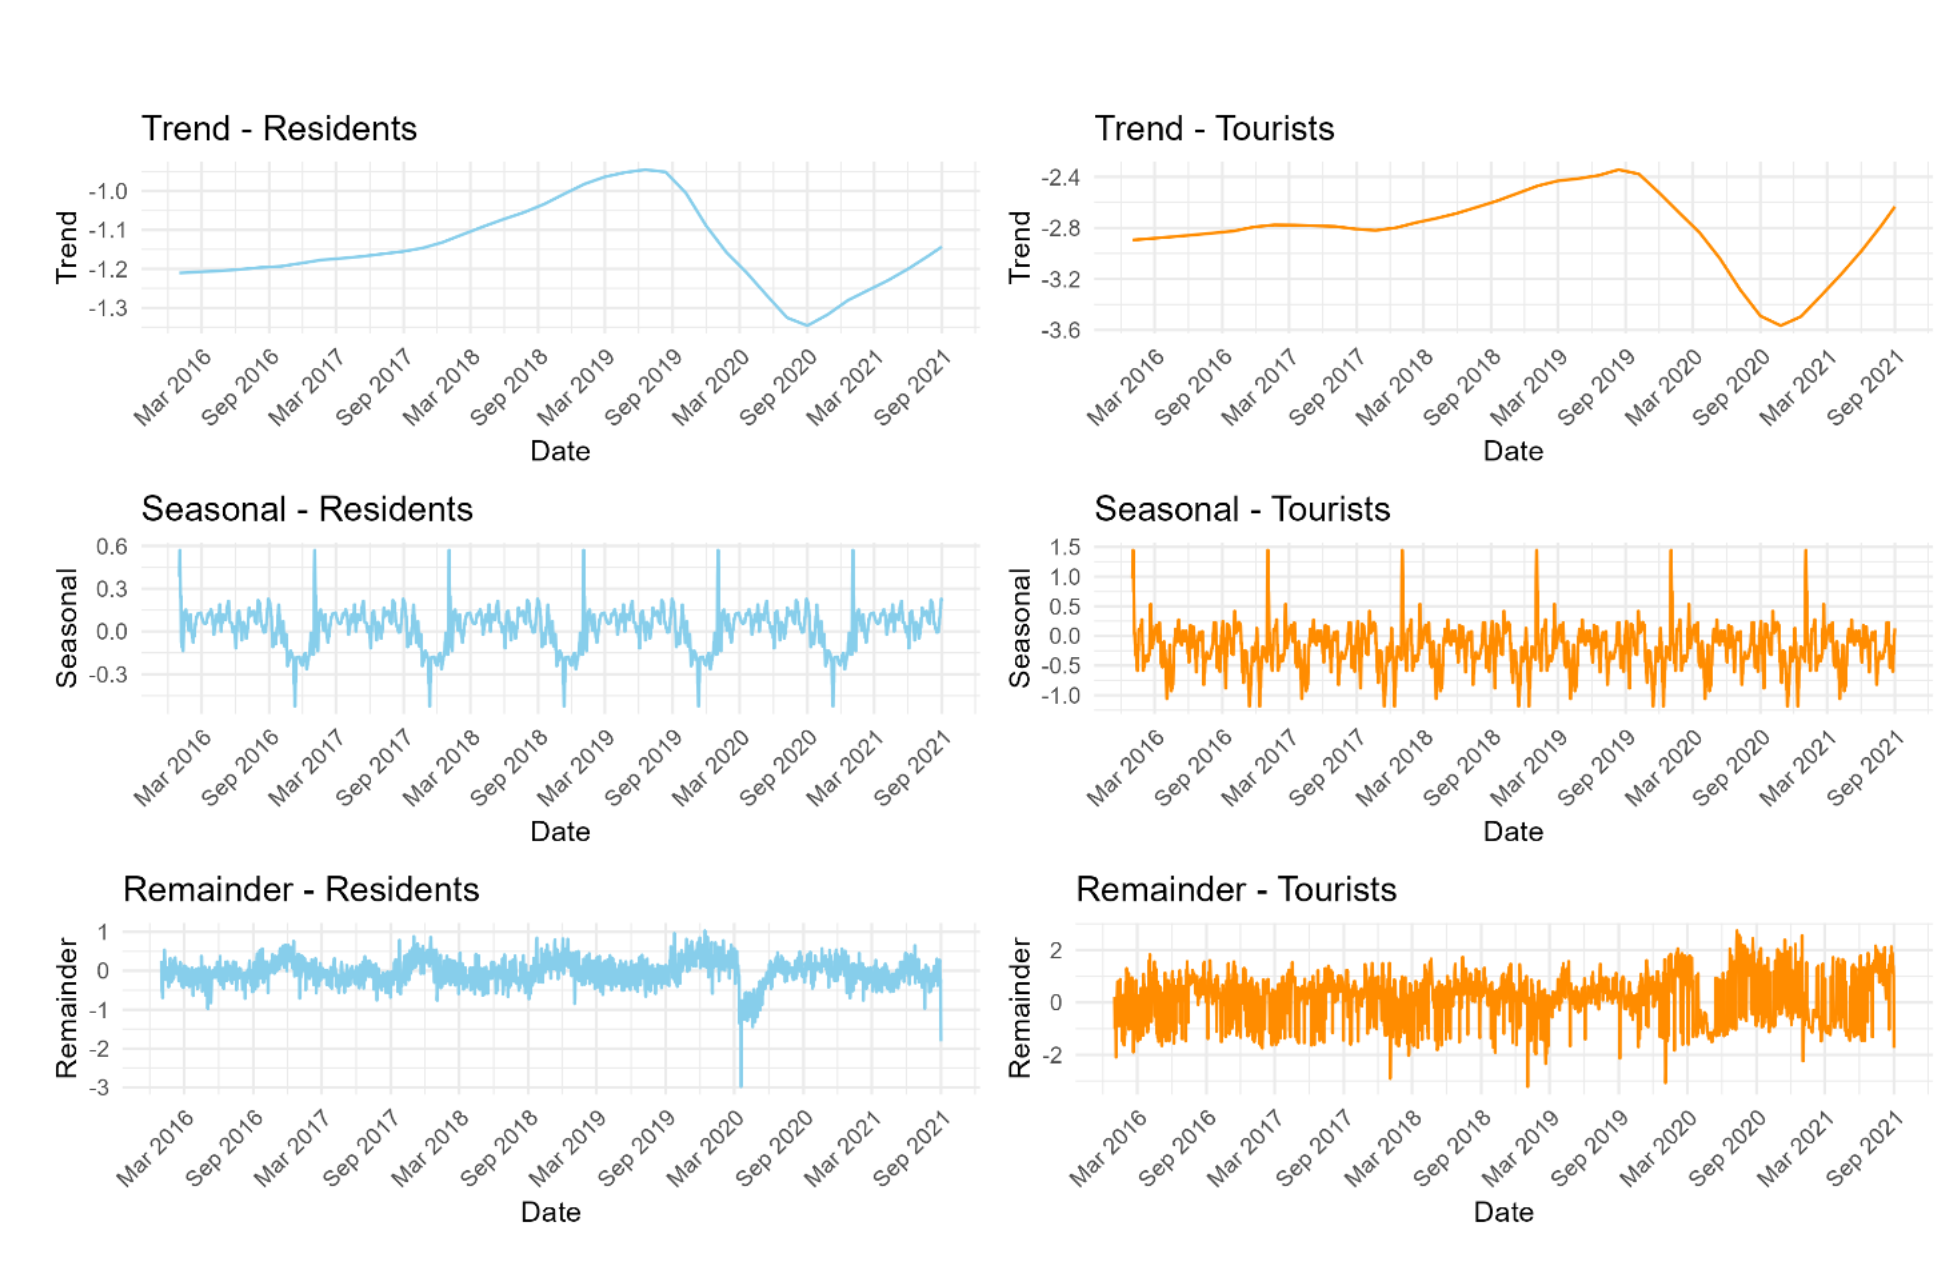
\includegraphics[keepaspectratio]{images/covidcrime.png}}

}

\caption{Series temporales de los robos en Barcelona, descomponiendo la
tendencia, el efecto estacional y el ruido. En la tendencia se puede
vislumbrar el descenso inducido por las restricciones de movilidad del
COVID. Fuente: Trinidad, Medina, y Marteache, 2024}

\end{figure}%

{[}MENCIONAR CAMBIOS TECNOLOGICOS Y LEGALES COMO DETERMINANTES{]}

Una de las cuestiones más debatidas en los últimos tiempos ha sido el
llamado \textbf{crime drop} (descenso del delito) y en qué grado este ha
sido un fenómeno generalizado.

Tanto en Estados Unidos como en el Reino Unido, las primeras potencias
criminológicas, el delito experimentó un muy visible descenso a partir
de la década de los 1990. En la siguiente figura podéis ver los datos de
la \emph{Crime Survey for England and Wales} durante este período.

\pandocbounded{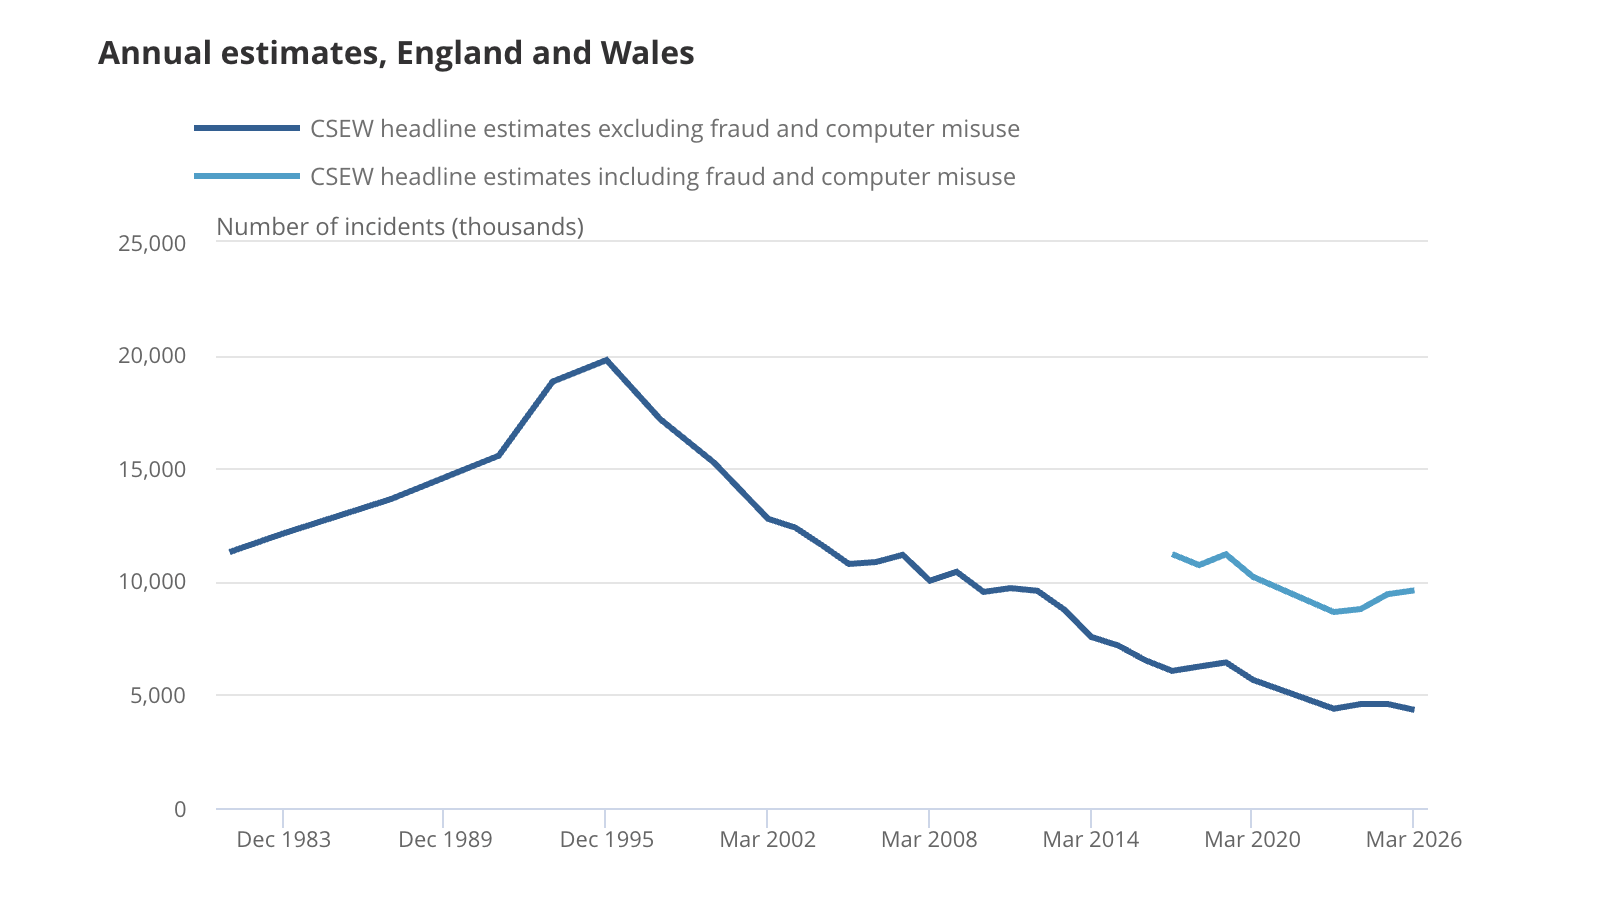
\includegraphics[keepaspectratio]{images/crimedrop.png}}
Como se puede observar hay un descenso notable del delito desde mediados
de los 90 hasta nuestros días en Inglaterra y Gales. ¿Por qué? ¿Es esta
una tendencia tambien observable en otros países? ¿En qué medida se ha
producido un desplazamiento hacia otro tipo de delitos que estos datos
no miden bien?

Empezemos por la última. Es verdad que las encuestas de victimación,
aunque (cuando bien hechas) son generalmente consideradas como el
instrumento más fiable para medir variaciones temporales en los niveles
globales de delincuencia (ya que no se ven afectadas por el sesgo de
denuncia), tradicionalmente no han medido delitos que a día de hoy se
han vuelto muy relevantes. La ciberdelincuencia, en particular, es la
forma delictiva del siglo XXI. Las encuestas de victimación, en su
mayoría, no han medido historicamente estas formas delictivas. La
\emph{Crime Survey for England and Wales} fue la primera encuesta
nacional que comenzó a experimentar y medir algunos de estos nuevos
delitos. En la gráfica mostrada arriba se puede ver como a partir del
2017 esta encuesta incluye medidas de ciberdelincuencia. El gráfico
muestra hasta que punto este tipo de delitos se ha convertido en un
elemento central para entender la delincuencia contemporanea.

¿Por qué se produce este descenso? Este ha sido un muy agrio debate en
el que no han faltado todo tipo de hipotesis que no resultan del todo
convincentes: cambios demográficos, cambios en los mercados de drogas,
variaciones en tácticas y estrategias policiales, economías más
saludables, la introducción del aborto, reducciones en los niveles de
exposición al plomo, cambios culturales, etc. (Blumstein y Wallman 2000;
Zimring 2011; Farrell, Tilley, y Tseloni 2010). Farrell et~al. (2008)
han propuesto como alternativa la \emph{hipótesis de la seguridad},
cambios en los niveles y prácticas ciudadanas y empresariales de
seguridad han podido ser un factor determinante. Ellos muestran análisis
que sugieren que la caída de dos tercios en los robos de automóviles en
el Reino Unido se debió en gran medida a las mejoras en los sistemas de
cierre centralizado e inmovilización y especulan que la adopción de otro
tipo de medidas de seguridad en el hogar y en las empresas puede haber
sido determinante en este sentido. Por lo que nos interesa, baste
señalar que entender los factores que pueden ser responsables de cambios
en los niveles de delincuencia es también una fructifera línea de
investigación dentro de la criminología.

\section{El delito a nivel micro}\label{el-delito-a-nivel-micro}

Al margen de estudiar el delito a nivel más macro y agregado para
entender su distribución temporal y espacial, a la criminología le
interesa entender el cómo y el porqué del delito a nivel más micro. En
esta sección introduciremos brevemente algunas ideas que han sido
importantes al considerar estas cuestiones.

\subsection{El delito como transacción
situacional}\label{el-delito-como-transacciuxf3n-situacional}

El concepto del delito como una «transacción situada» fue desarrollado
notablemente por David F. Luckenbill, quien analizó los homicidios como
secuencias de interacciones entre el agresor y la víctima. Una
«transacción situada» se refiere a una cadena de interacción entre dos o
más individuos que dura el tiempo que se encuentran en la presencia
física inmediata unos de otros. Luckenbill (1977) descubrió que el
asesinato suele ser el resultado de una serie de intercambios cada vez
más intensos ---lo que Goffman denominó «competición de caracteres»---
en los que cada parte busca mantener o recuperar su «prestigio» mediante
desafíos verbales y físicos. El resultado (por ejemplo, el homicidio)
viene determinado por el contexto social inmediato y las acciones de
todos los implicados, y no solo por la intención o los antecedentes
individuales. Investigaciones posteriores respaldan esta opinión,
demostrando que muchos delitos violentos, especialmente los homicidios,
se desarrollan como procesos interactivos.

\begin{tcolorbox}[enhanced jigsaw, bottomtitle=1mm, toprule=.15mm, colbacktitle=quarto-callout-note-color!10!white, bottomrule=.15mm, leftrule=.75mm, colframe=quarto-callout-note-color-frame, opacitybacktitle=0.6, titlerule=0mm, breakable, colback=white, left=2mm, arc=.35mm, title=\textcolor{quarto-callout-note-color}{\faInfo}\hspace{0.5em}{Nota}, toptitle=1mm, coltitle=black, rightrule=.15mm, opacityback=0]

\textbf{La teoría de las acciones coercitivas}

Tedeschi y Felson (1994) desarrollaron toda una teoría de la violencia
inspirados en parte por este modelo. La teoría de la violencia de
Tedeschi y Felson, denominada \emph{teoría interaccionista social de las
acciones coercitivas}, estructura y secuencia las situaciones violentas
centrándose en el daño como comportamiento orientado a objetivos que
surge de procesos interaccionistas sociales. Siguiendo a Bandura
consideran que toda violencia se considera instrumental y mediada
cognitivamente, rechazando la ``agresión enfadada'' automática asociada
a las teorías que distinguen entre violencia instrumental y expresiva.La
teoría describe tres motivos sociales principales que inician y dan
forma a los episodios coercitivos:

\begin{itemize}
\item
  Influir en otros para obtener beneficios: esto incluye obtener bienes,
  servicios o seguridad.
\item
  Expresar quejas y establecer la justicia: este motivo está asociado
  con atribuciones de culpa, ira y sentimientos de injusticia, lo que a
  menudo conduce a acciones punitivas.
\item
  Afirmar o defender identidades sociales: la coacción puede ser una
  táctica de autopresentación para mantener una imagen favorable (por
  ejemplo, fuerte, valiente) o para evitar parecer débil.
\end{itemize}

Cómo Luckenbill (1977), Tedeschi y Felson (1994) conceptualizan las
situaciones coercitivas como dinámicas, implican una serie de decisiones
y respuestas. Por ejemplo, en las coacciones reactivas el proceso
secuencial suele comenzar con la percepción de una violación de las
normas y una injusticia. Esto lleva a atribuir la culpa al autor, lo que
a su vez provoca ira. Los agravios pueden expresarse entonces mediante
reproches, reclamaciones de medidas correctivas o negociaciones. Las
perspectivas divergentes entre los actores y los objetivos (los autores
minimizan el daño, las víctimas lo exageran) pueden intensificar los
conflictos.

Cuando las quejas se expresan con dureza o se rechazan, las hostilidades
pueden intensificarse. Los ataques a la identidad (insultos, críticas)
son especialmente propensos a provocar «espirales de conflicto», en las
que cada contraataque degrada aún más al otro, lo que a veces da lugar a
violencia física. El alcohol y las emociones fuertes pueden exacerbar
esto al deteriorar los controles cognitivos y aumentar la propensión al
riesgo.

Igualmente, la presencia de terceros puede influir significativamente en
la secuencia de la violencia. Pueden disuadir la delincuencia actuando
como guardianes, pero también pueden exacerbar el conflicto al aumentar
las preocupaciones identitarias, incitar a los antagonistas o tomar
partido.

\end{tcolorbox}

Si bien el modelo de «transacción situada» se aplica más directamente a
los delitos violentos entre personas, algunas teorías criminológicas
amplían la idea a otras formas de delito, haciendo hincapié en la
importancia de los contextos sociales, emocionales y físicos inmediatos
en la configuración del comportamiento delictivo y sus consecuencias.

En este sentido Horney (2006), en su discurso inaugural como presidenta
de la \emph{American Society of Criminology} proponía que para
comprender el comportamiento delictivo es más útil hacer hincapié en la
especificidad de la situación que centrarse únicamente en los rasgos de
personalidad estables de las personas. Horney (2006) destaca como las
señales ambientales influyen en las acciones y critica las teorías
tradicionales de la personalidad basadas en los rasgos, haciendo
referencia al trabajo de Walter Mischel sobre las contingencias
situacionales del comportamiento. Horney propone que la criminalidad
debe considerarse como el resultado del vínculo inextricable entre las
situaciones y el comportamiento, e insta a los criminólogos a tener en
cuenta las consistencias ambientales y a recopilar datos situacionales
en sus investigaciones, especialmente en los estudios sobre el curso de
la vida, para comprender mejor la complejidad de las acciones humanas.

\subsection{Toma de decisiones}\label{toma-de-decisiones}

La toma de decisiones de los delincuentes se ha explicado
tradicionalmente mediante la teoría de la elección racional, que postula
que los individuos sopesan los costes y beneficios del delito antes de
actuar. Sin embargo, las investigaciones demuestran que este proceso
suele estar «limitado» por la escasez de información, tiempo y recursos
cognitivos, lo que conduce a decisiones que no son del todo racionales
(Bernasco, Gelder, y Elffers 2017). La economía conductual
(\emph{behavioural economics}) y los modelos de doble sistema o proceso
(Kahneman 2011) resaltan además que los delincuentes usan heurísticas
(atajos mentales) y se ven influenciados por sesgos, emociones y
factores situacionales.

Las teorías de la elección racional se remontan a los inicios del
pensamiento criminológico con Beccaria y Bentham. Bentham, en
particular, proponía que cada acción humana podía evaluarseen términos
de la cantidad de placer o dolor que producía. El delito era simplemente
una acción en la que el actor había evaluado que los beneficios
superaban los costos. La función del legislador, por tanto, consistía en
diseñar un sistema de sanciones que reequilibrara esa ecuación, dejando
que delito dejara de producir más placer que dolor.

El renacimiento del paradigma racionalista se dio con el artículo de
Gary S. G. Becker (1968), \emph{Crime and Punishment: An Economic
Approach}, que introdujo un marco microeconómico para explicar la
conducta delictiva. Becker modeló la delincuencia como un cálculo de
utilidad esperada: una persona compara los beneficios de un acto ilegal
con sus costos, que incluyen la probabilidad de ser descubierto y la
severidad del castigo, además de los costos de oportunidad (por ejemplo,
los salarios legales perdidos). Se comete el delito si la recompensa
esperada es mayor que la alternativa legal; si no lo es, no se comete.
También planteó el problema de la sociedad: elegir el esfuerzo de
aplicación de la ley (probabilidad de sanción) y la gravedad del castigo
para minimizar la pérdida social total (daño por el delito + costos de
aplicación + costos de sanción).

\begin{figure}

\begin{minipage}{0.73\linewidth}
\pandocbounded{
\includegraphics[keepaspectratio]{images/becker.webp}}\end{minipage}%
%
\begin{minipage}{0.27\linewidth}
\pandocbounded{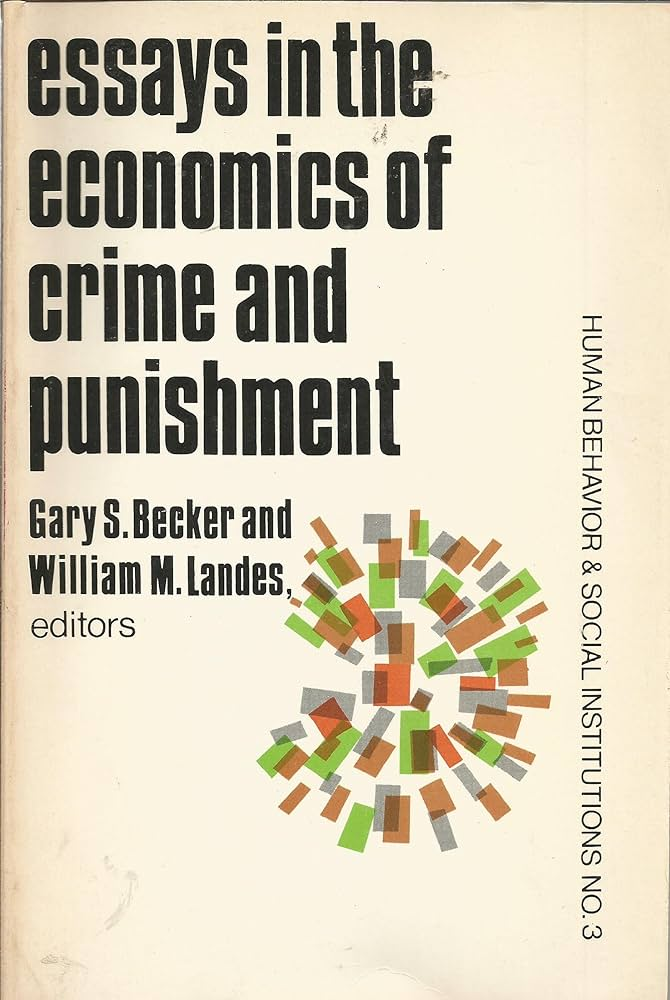
\includegraphics[keepaspectratio]{images/garybecker.jpg}}\end{minipage}%
\newline
\begin{minipage}{0.50\linewidth}
Gary Becker\end{minipage}%

\end{figure}%

Sin embargo, el modelo de Becker fue objeto de críticas importantes:

\begin{itemize}
\item
  Racionalidad perfecta: se asume que los delincuentes tienen
  información completa y capacidad de cálculo preciso, lo cual rara vez
  ocurre.
\item
  Neutralidad frente al riesgo: la teoría no contempla aversión o
  propensión al riesgo.
\item
  Miopía temporal: los individuos suelen descontar fuertemente el
  futuro, lo que reduce la eficacia de sanciones lejanas.
\item
  Desigualdad estructural: la teoría trata el crimen como elección
  individual y deja en segundo plano factores sociales.
\end{itemize}

Aun con estas críticas, el artículo de Becker revitalizó el enfoque
racionalista, inspirando no solo investigaciones empíricas, sino toda
una corriente de análisis económico del derecho.

Ante las críticas al modelo económico puro, criminólogos como Derek
Cornish y Ronald Cornish y Clarke (1968) (\emph{The Reasoning Criminal})
propusieron una versión más matizada: la teoría de la racionalidad
acotada (\emph{bounded rationality}). Según ellos, los delincuentes sí
actúan con intencionalidad y propósito, pero su racionalidad está
limitada por información incompleta, presiones situacionales y sesgos
cognitivos. En lugar de imaginar al delincuente como un calculador
abstracto, Cornish y Clarke lo describieron como un actor que toma
decisiones prácticas en contextos concretos: elegir una casa sin alarma
para robar, evitar lugares muy vigilados, preferir delitos de bajo
esfuerzo. Estudios empíricos de ladrones de coches o carteristas
muestran que efectivamente ponderan riesgos inmediatos y oportunidades
visibles, aunque de manera rápida y heurística, más que mediante
cálculos precisos. Esta transición de la racionalidad absoluta a la
racionalidad acotada supuso un avance teórico, permitiendo incorporar
hallazgos de la psicología cognitiva.

\begin{figure}

\begin{minipage}{0.59\linewidth}
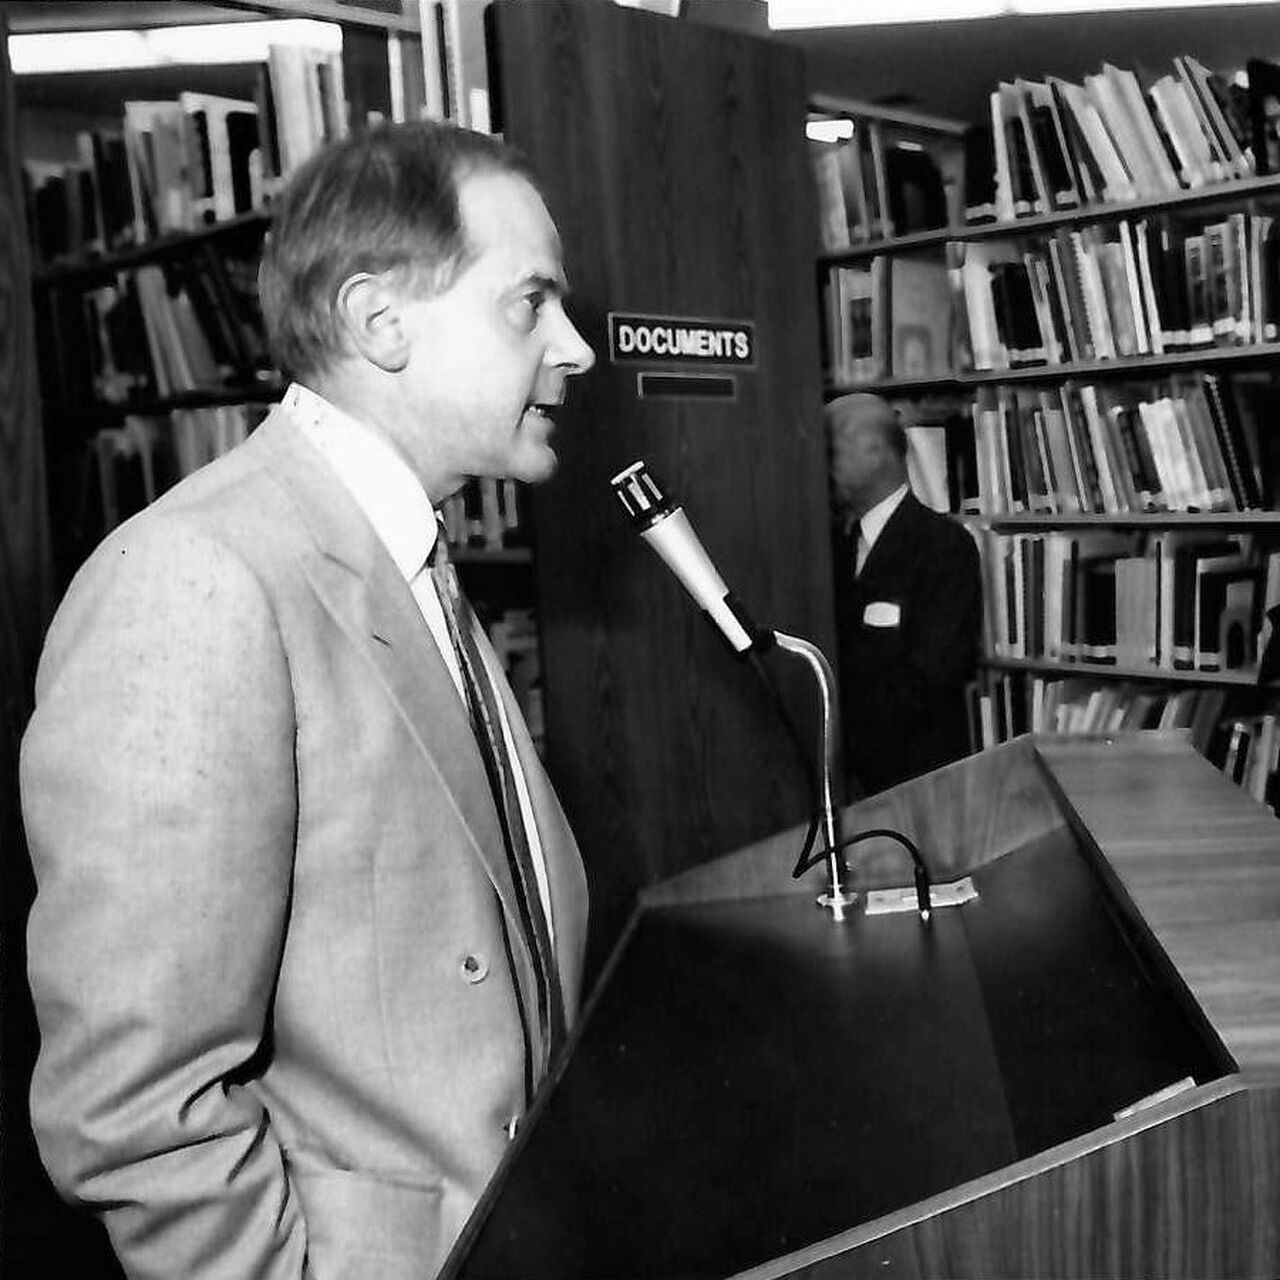
\includegraphics[width=3in,height=\textheight,keepaspectratio]{images/ronaldclarke.jpg}\end{minipage}%
%
\begin{minipage}{0.41\linewidth}
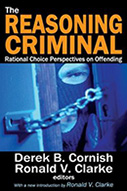
\includegraphics[width=2.05in,height=\textheight,keepaspectratio]{images/the-reasoning-criminal.jpg}\end{minipage}%
\newline
\begin{minipage}{0.50\linewidth}
Ronald Clarke\end{minipage}%

\end{figure}%

En las últimas décadas, la perspectiva de la elección racional ha sido
enriquecida por aportes de la psicología del juicio y la toma de
decisiones y de la neurociencia. Estos refinamientos no niegan que el
delito sea, en parte, una decisión, pero muestran que esa decisión está
plagada de sesgos, limitaciones y particularidades cognitivas. Kahneman
y Tversky (1979), por ejemplo, demostraron que los individuos no evalúan
probabilidades de manera lineal. Tienden a sobrestimar probabilidades
bajas y a subestimar probabilidades altas. Para el delincuente, esto
implica que el ``riesgo de ser atrapado'' puede ser percibido de manera
distorsionada: algunos lo magnifican, otros lo minimizan casi hasta
ignorarlo.

La investigación en economía conductual también muestra que los
individuos aplican un descuento hiperbólico al futuro: prefieren
recompensas inmediatas aunque sean pequeñas frente a castigos o
beneficios lejanos. Esto explica por qué las sanciones diferidas ---como
una pena de cárcel que llegará tras un largo proceso--- tienen un poder
disuasorio menor.

El trabajo de Kahneman ha sido importante en el desarrollo de la teoría
del proceso dual. Kahneman (2011) distingue entre dos modos de
procesamiento cognitivo:

\begin{itemize}
\item
  El \emph{Sistema 1}: rápido, automático, intuitivo, basado en
  heurísticos y emociones. Funciona sin esfuerzo consciente.
\item
  El \emph{Sistema 2}: lento, deliberativo, analítico, capaz de cálculos
  complejos y de anticipar consecuencias a largo plazo.
\end{itemize}

Ambos sistemas interactúan constantemente, pero no de manera simétrica:
el Sistema 1 domina la mayoría de decisiones cotidianas, y el Sistema 2
interviene solo cuando se requiere un esfuerzo adicional.

\begin{figure}

\begin{minipage}{0.68\linewidth}
\pandocbounded{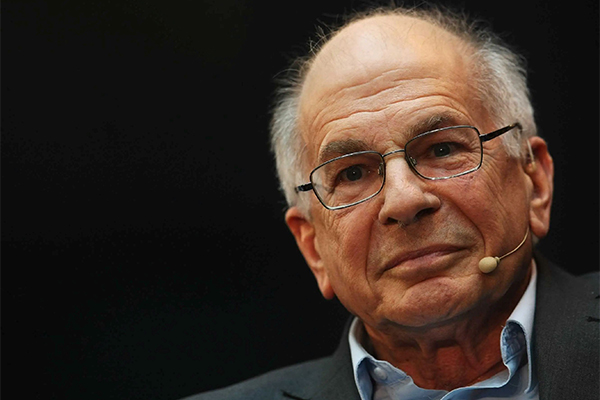
\includegraphics[keepaspectratio]{images/Daniel-Kahneman.jpg}}\end{minipage}%
%
\begin{minipage}{0.32\linewidth}
\pandocbounded{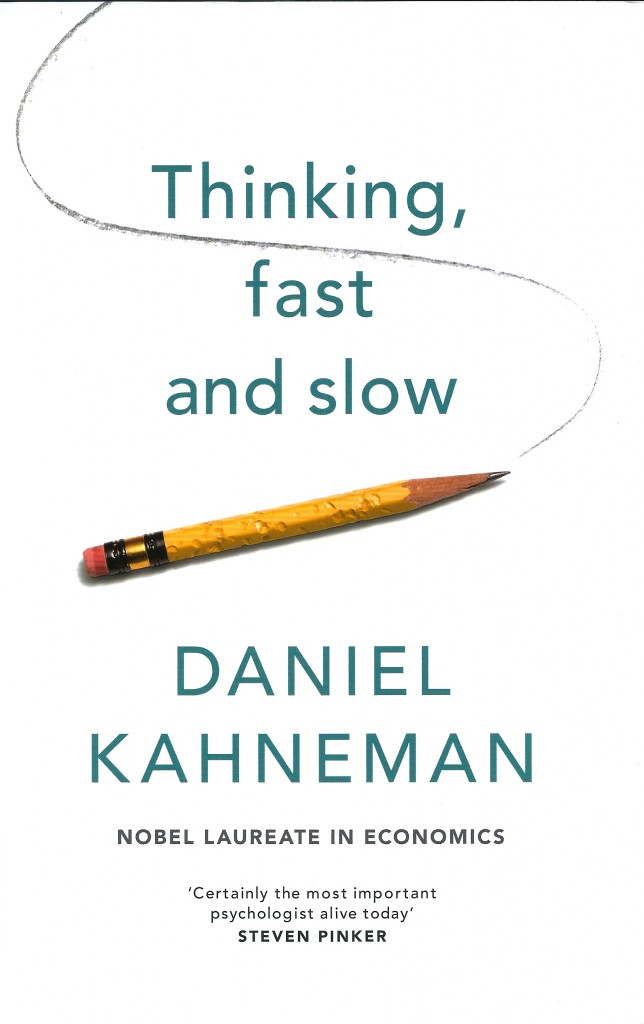
\includegraphics[keepaspectratio]{images/thinking.jpg}}\end{minipage}%
\newline
\begin{minipage}{0.50\linewidth}
Daniel Kahneman\end{minipage}%

\end{figure}%

Muchos delitos ---peleas, robos oportunistas, vandalismo--- ocurren en
contextos de alta emocionalidad, presión social o búsqueda inmediata de
gratificación. En estos casos puede predominar el Sistema 1: rápido,
emocional y miopemente enfocado en la recompensa inmediata. Por el
contrario, en otros delitos en los que puede haber más planificación
---fraudes financieros, robos organizados, corrupción--- se apreciará
más facilmente la activación del Sistema 2. El delincuente evalúa
opciones de forma más consciente, calcula riesgos, planifica la
ejecución y anticipa medidas de evasión. La evidencia de entrevistas con
delincuentes de cuello blanco o con ladrones profesionales muestra que
analizan costes de seguridad, probabilidad de captura y ganancias
esperadas. Esto es, en todo caso, un ejemplo simplificado sólo a efectos
expositivos. En la práctica los dos sistemas no operan de forma aislada.
Incluso delitos que nos pueden parecer planificados, por ejemplo, a
menudo se cometerán en modo pilóto automático.

Resumiendo algunas de estos cuestiones, la evidencia viene a mostrar
apoyo a las siguientes cuestiones en la toma de decisiones por parte de
los delincuentes (Bernasco, Gelder, y Elffers 2017):

\begin{itemize}
\item
  \emph{Racionalidad ajustada o limitada}. La mayoría de los
  delincuentes cuando hacen calculos de costos y beneficios lo hacen con
  información limitada, condicionados por el tiempo, y adoptando atajos
  mentales. A menudo le dan más importancia a los beneficios inmediatos
  mientras que descuentan las consecuencia a largo plazo (el sesgo del
  presente).
\item
  \emph{Los factores situacionales}. La toma de decisiones puede verse
  muy influenciada por contingencias situacionales inmediatas. Muchos
  delitos son oportunistas, están provocados por señales situacionales
  como un coche sin cerrar o una propiedad desatendida.
\item
  \emph{Sesgos cognitivos}. Los delincuentes exhiben sesgos sistemáticos
  cuando toman decisiones, incluyendo un exceso de confianza en su
  capacidad para evitar ser detectados, un optimismo poco realista sobre
  los resultados y una evaluación deficiente de los riesgos. Tienden a
  sobreestimar las ganancias potenciales y a subestimar tanto la
  probabilidad como la gravedad del castigo.
\item
  \emph{Aprendizaje y adaptación}. Los delincuentes experimentados
  aprenden de sus experiencias pasadas, volviéndose más sofisticados en
  la selección de objetivos y en la evitación de riesgos. Sin embargo,
  esta experiencia criminal suele ser específica de cada ámbito y no se
  traduce necesariamente en una mejor toma de decisiones en general.
\item
  \emph{Diferencias individuales}. Factores que varían entre individuos
  como la impulsividad, el abuso de sustancias tóxicas o el alcohol,
  problemas de salud mental, el autocontrol, y las habilidades
  cognitivas generan variación sustancial en la calidad de la toma de
  decisiones por parte de los delincuentes. Algunos delincuentes son más
  propensos a actuar de forma impulsiva que otros.
\item
  \emph{Las influencias sociales y emocionales}. Las dinámicas sociales,
  como el pensamiento grupal (\emph{group think}), la gestión de la
  reputación dentro de las redes criminales y la necesidad de mantener
  el estatus, influyen significativamente en las decisiones. Del mismo
  modo, como veremos con más detalle en la siguiente sección, las
  decisiones criminales se toman bajo la influencia de emociones
  intensas, como la ira, la desesperación o la presión de los
  compañeros.
\end{itemize}

En resumen, a lo largo del tiempo hemos ido desarrollando un apreciacion
de la toma de decisiones por parte de los delincuentes como un proceso
complejo, en el que interactuan varios elementos, y que no se conforma a
las visiones más puras o primitivas de una elección racional. Es
evidente que existe una instrumentalidad a la hora de delinquir que es
muy relevante, pero no podemos simplificar lo que esto implica.

\subsection{Emoción, significado y
delito}\label{emociuxf3n-significado-y-delito}

Las emociones suelen estar poco teorizadas en las principales teorías
sobre la delincuencia. Sin embargo, las emociones pueden actuar tanto
como motivadoras como reguladoras del comportamiento delictivo. Cada vez
se reconoce más que las emociones y las cogniciones influyen de manera
continua y recíproca en los juicios, las decisiones y las conclusiones
que alcanzamos. Como señala Nee (2025, 575):

\begin{quote}
``El llamamiento a una comprensión más clara de las influencias
emocionales en la toma de decisiones delictivas no es nuevo y ha ido
cobrando impulso durante varios años\ldots{} Esto se ha visto impulsado
en parte por una apreciación más profunda de la naturaleza y la relación
entre la cognición y la emoción. Los investigadores en psicología,
neurociencia y filosofía han (1) abandonado la visión de que el cerebro
y el cuerpo son entidades distintas, para reconocer que todo nuestro
cuerpo participa en la adquisición de conocimientos y experiencias (lo
que se conoce como cognición incorporada) y (2) han reconocido que la
emoción es un aspecto crucial y plenamente integrado del procesamiento
de la información y la percepción.''
\end{quote}

Los delincuentes suelen experimentar una serie de emociones durante la
comisión del delito, como euforia, calma, angustia o depresión, que
pueden influir en sus acciones y en sus procesos de toma de decisiones.
``Las emociones parecen desempeñar un importante papel facilitador y
motivador en la delincuencia, y no solo desinhibidor'' (Nee 2025, 582).
Por ejemplo, algunos delincuentes pueden sentirse empoderados o
justificados (héroe eufórico, profesional tranquilo), mientras que otros
pueden actuar por angustia o victimización (vengador angustiado, víctima
deprimida).

Estos estados emocionales no solo son respuestas al acto, sino que
también pueden impulsar la decisión inicial de cometer un delito. La ira
y el miedo influyen especialmente en la comisión de delitos violentos, y
estudios experimentales y basados en encuestas demuestran que estas
emociones pueden aumentar directamente la intención de delinquir y
moderar el impacto de la deliberación racional. Como vereis cuando
estudieis teorias criminologicas, la teoría general del estrés de Robert
Agnew postula que las emociones negativas derivadas del estrés o la
tensión (por ejemplo, la ira o la depresión) median la relación entre
las experiencias adversas y el comportamiento delictivo.

Algunos estudios sugieren que diferentes subconjuntos de delitos se
asocian más con diferentes emociones. Canter y Ioannou (2004), por
ejemplo, encontraba en un estudio con una muestra de 83 delincuentes
encarcelados que los delitos contra la propiedad resultaban más
placenteros que los delitos contra las personas.

\begin{tcolorbox}[enhanced jigsaw, bottomtitle=1mm, toprule=.15mm, colbacktitle=quarto-callout-note-color!10!white, bottomrule=.15mm, leftrule=.75mm, colframe=quarto-callout-note-color-frame, opacitybacktitle=0.6, titlerule=0mm, breakable, colback=white, left=2mm, arc=.35mm, title=\textcolor{quarto-callout-note-color}{\faInfo}\hspace{0.5em}{Nota}, toptitle=1mm, coltitle=black, rightrule=.15mm, opacityback=0]

\textbf{Jack Katz y la seducción moral del delito}

Jack Katz publicó a finales de los 80 un influyente trabajo que
reinvicaba el estudio de las emociones. En \emph{Seductions of Crime}
(Katz 1988), se argumenta que el papel de las emociones en el crimen es
central. Katz (1988) señala que la investigación criminológica ha estado
preocupada por la búsqueda de fuerzas de trasfondo como defectos
psicológicos o entornos sociales, descuidando las atracciones positivas,
a menudo ``maravillosas'', dentro de la experiencia vivida de la
criminalidad. El trabajo de Katz se centra en las cualidades seductoras
de los crímenes, destacando cómo varias formas de criminalidad son
``sensualmente atractivas''.

Katz postula que la naturaleza misma del ser mundano es emocional; la
atención es sentimiento, y la conciencia es sensual. La criminalidad no
es meramente una reacción contra las estructuras sociales, sino que
posee una genuina creatividad experiencial. La atracción más convincente
en muchas experiencias desviadas es superar un desafío personal a la
existencia moral, no material.

Algunas emociones clave y su manifestación en el delito incluirían:

\begin{itemize}
\item
  \emph{Humillación y rabia}: En los asesinatos apasionados, que él
  denomina ``sacrificio justiciero'' (``righteous slaughter''), el
  proceso emocional implica transformar una ``situación eternamente
  humillante en rabia''. El asesino interpreta las acciones de la
  víctima como un ataque a un ``valor humano eterno'' y a su propia
  valía fundamental, lo que lleva a una ``última resistencia'' en
  defensa de la respetabilidad. Esta rabia permite al asesino cegarse a
  su futuro, forjando un sentido momentáneo de unidad eterna con el
  bien. La humillación y la rabia se consideran ``sentimientos
  holísticos'' donde el individuo se experimenta a sí mismo como
  impulsado por fuerzas más allá de su control, y la rabia está viva con
  la conciencia de la humillación. El cambio de humillación a rabia
  puede ser rápido porque comparten características fundamentales y se
  reflejan inversamente.
\item
  \emph{Emociones furtivas}: El hurto en tiendas, el robo con
  allanamiento y el vandalismo se describen como ofertas de ``sneaky
  thrills'' (emociones furtivas) que no están impulsadas por recompensas
  materiales obvias. En cambio, proporcionan una forma ``mágica'' de
  ocultar y poner a prueba deseos censurados. Estas emociones implican
  una ``euforia'', un sentido de ``profanación secreta'' (usando una
  metáfora religiosa), y pueden ser ``eróticamente evocadoras'' (usando
  una metáfora sexual). La emoción proviene de jugar con las apariencias
  y coquetear con la desviación, probando los límites del yo.
\item
  \emph{Pavor y crueldad}: Individuos que encarnan la personalidad de
  ``malote'' (``badass'') o pertenecen a ``élites callejeras'' buscan
  mostrar dominancia y una indiferencia a las expectativas de la
  sociedad moderna. Cultivan un ``aura de pavor'' a través de la
  violencia y acciones simbólicas, buscando imponer su ``significado''
  sin consideraciones utilitarias. Emociones como la arrogancia, el
  ridículo, el cinismo, la profanación y la venganza son parte integral
  de estos proyectos. Ser ``cool'' o ``ser animal'' son formas de
  manifestar esta identidad ajena y sugerir ``posibilidades caóticas''.
\item
  \emph{Suspense y dureza}: Los atracadores, particularmente los
  ``hombres duros'', enfrentan dificultades existenciales significativas
  y suspense una vez que declaran un atraco. Deben desarrollar una
  ``incompetencia moral distintiva'' y una ``indiferencia a las
  consecuencias mundanas'' de sus acciones. Para persistir en el atraco,
  cultivan una ``dureza'' y una ``maldad moral'', impulsadas por el
  compromiso de que su voluntad prevalezca, independientemente del
  interés propio práctico. La violencia, incluso cuando parece
  ``irracional'', puede ser instrumental para construir una reputación
  de ``malote'' y asegurar su posición entre sus compañeros. La
  seducción es provocada por las atracciones existenciales de ser
  ``malo'' como una forma de ser celebrada colectivamente que trasciende
  el bien y el mal.
\item
  \emph{Vértigo y mal primordial}: Los asesinatos descritos como
  asesinatos sin sentido y a sangre fría están motivados por una
  preocupación por cuestiones morales y una seducción por las
  atracciones del mal primordial. La dinámica emocional se caracteriza
  por un ``vértigo'' donde los individuos oscilan entre un compromiso
  lúdico con el simbolismo desviado y una ``vergüenza paranoica en la
  conformidad''. La naturaleza ``sin sentido'' de estos asesinatos,
  donde hay poca ganancia material y las víctimas a menudo no se
  resisten, desafía la comprensión convencional. Para los perpetradores,
  se convierte en un acto positivo de reclamar su estatus como un
  desviado impresionante, una ``resolución creativa'' de su
  incertidumbre moral, donde infligen sufrimiento para escribir en la
  sangre de sus víctimas la historia de la falta de respeto y la falta
  de fe con la que otros los habían profanado. Esto a menudo refleja una
  ``crisis de comprensión'' para los propios asesinos, quienes pueden
  cuestionar su propia normalidad después del acto.
\end{itemize}

En esencia, Katz argumenta que comprender las diversas experiencias
emocionales ---que van desde la rabia y las emociones fuertes hasta el
pavor, el suspense y una vertiginosa aceptación del mal--- es crucial
para entender por qué la gente comete crímenes, yendo más allá de las
explicaciones simplistas materialistas o centradas en la personalidad o
el ambiente social de los delincuentes.

\end{tcolorbox}

\subsection{El cómo del delito: los guiones del delito (crime
scripts)}\label{el-cuxf3mo-del-delito-los-guiones-del-delito-crime-scripts}

A la criminología también le motiva el entender de qué forma se cometen
los delitos, el desarrollar descripciones adecuadas de la forma en que
se articulan los mismos. Hay una larga tradición de investigación
cualitativa que ha profundizado en estas cuestiones. Más recientemente
se ha propuesto una herramienta, los guiones delictivos o \textbf{crime
scripts} para sistematizar el modus operandi.

Un guion delictivo es un modelo sistemático y procedimental que describe
la secuencia de acciones, decisiones y acontecimientos que intervienen
en la comisión de un tipo específico de delito. Son descripciones
abstractas de un tipo particular de proceso conductual, es decir,
secuencias estructuradas de comportamiento que se extienden en el tiempo
y quizás en el espacio, que podrían considerarse unidades o subunidades
funcionalmente autónomas de secuencias más largas.

Fue introducido por primera vez por (\textbf{Cornish\_?}) y se ha
convertido en una herramienta muy utilizada en criminología para
analizar el modus operandi (métodos) de los delincuentes e identificar
puntos de intervención para la prevención del delito. Los guiones
delictivos ayudan a descomponer delitos complejos en etapas distintas,
como la preparación, la ejecución y las actividades posteriores al
delito, lo que facilita la comprensión del comportamiento del
delincuente y el diseño de estrategias de prevención específicas. Este
enfoque ofrece un valor significativo a los analistas criminales, ya que
sirve como herramienta para ``obtener información sobre el
comportamiento del delincuente y los motivos de sus decisiones'' y para
``organizar los conocimientos existentes sobre los requisitos para
cometer un delito, como las habilidades o los recursos que los
delincuentes necesitan desplegar para ejecutar un delito'' (Dehghanniri
y Borrion 2019, 2).

Un guion delictivo suele constar de los siguientes elementos (Chainey y
Alonso-Berbotto 2022):

\begin{itemize}
\item
  \emph{Actos}: son las etapas clave del proceso de comisión del delito.
\item
  \emph{Escenas}: describen los escenarios en los que se producen los
  actos. Tompson y Chainey (2011) simplificaron las clasificaciones
  originales de Cornish en cuatro categorías principales: «preparación;
  preactividad; actividad y postactividad».
\item
  \emph{Reparto de actores}: se refiere a los participantes, personas u
  organizaciones, y a las funciones que desempeñan en cada escena.
\item
  \emph{Condiciones}: describen las circunstancias que influyen en la
  actividad delictiva y se desglosan en:

  \begin{itemize}
  \item
    Requisitos previos: condiciones que deben cumplirse antes de que
    comience la actividad ilegal.
  \item
    Facilitadores: factores que hacen que la actividad sea más fácil y
    rentable.
  \item
    Condiciones de aplicación: legislación, reglamentos y licencias que
    rigen el acto.
  \end{itemize}
\end{itemize}

Los guiones pueden completarse utilizando diversas fuentes de datos,
como expedientes de casos, entrevistas e inteligencia de fuentes
abiertas, y se utilizan para analizar delitos que van desde el crimen
organizado y el terrorismo hasta el fraude y el narcotráfico. Este
enfoque es especialmente valioso para la prevención situacional del
delito, ya que destaca puntos específicos en los que las intervenciones
pueden interrumpir el proceso delictivo. Para más detalles podéis leer
en castellano a Arenas (2024).

{[}INSERTAR ALGÚN EJEMPLO{]}

\chapter{El delincuente}\label{el-delincuente}

\section{Participación en actividades
delictivas}\label{participaciuxf3n-en-actividades-delictivas}

\subsection{El hombre delincuente}\label{el-hombre-delincuente}

La criminología que se desarrolla a partir del siglo XIX estaba
obsesionada con identificar los marcadores que nos permitirían
distinguir al hombre delincuente. A las personas nos gusta pensar en
términos de blancos y negros, de malos y buenos, de fronteras claramente
demarcadas entre lo diabólico y lo divino. La realidad, como veremos, es
obstinadamente más compleja.

Durante el siglo XIX, cuando irrumpen las primeras explicaciones
``científicas'' del comportamiento criminal, la naciente psiquiatría:

\begin{quote}
``intentaba explicar por qué algunos delincuentes parecían
imperturbables y especialmente crueles. Una y otra vez, estos
psiquiatras volvían al enigma de las personas que cometían delitos
repetidamente, a veces de forma obsesiva, sin importar el castigo o el
tratamiento que recibieran. Descubrieron que estas personas tienden a
cometer delitos espantosos y despiadados, lo que supuestamente
demostraba su incapacidad para identificarse con sus víctimas. \emph{La
criminología comenzó con los esfuerzos por comprender científicamente
este tipo de delincuentes}. Los teóricos utilizaron diferentes términos
para identificar la condición que causaba la reincidencia, aparentemente
incontrolable: trastorno moral, locura moral, manía sin delirio,
degeneración, imbecilidad moral, incorregibilidad, criminalidad innata,
incapacidad hereditaria. Pero aunque las etiquetas diferían, el objetivo
era el mismo: explicar las acciones de los delincuentes moralmente
dementes. Los teóricos concluyeron que la locura moral era un estado o
condición'' (Rafter 2011, 149)
\end{quote}

Los teóricos del siglo XIX que comenzaban a reflexionar sobre el hombre
delincuente pensaban que este comportamiento repetido era el producto de
una condición innata y que quienes sufrían de ella carecían de sentido
moral. Esta locura moral se pensaba como una deficiencia o condición
biológica.

Aunque ni mucho menos fue el único autor en pensar en estos términos,
suele citarse al médico italiano Cesare Lombroso (1885-1909) como
particularmente influyente en la cristalización de estas ideas. Lombroso
publicó en 1876 su influyente libro \emph{L'uomo delinquente}. Lombroso
proponía que el hombre delincuente, en particular lo que el llamaba el
\textbf{delincuente nato}, se distinguía del resto de los mortales por
una serie de anomalías físicas y que, influenciado por las teorias de la
evolución de Darwin, representaban una reversión a una forma primitiva
de ser humano.

\begin{figure}[H]

{\centering \pandocbounded{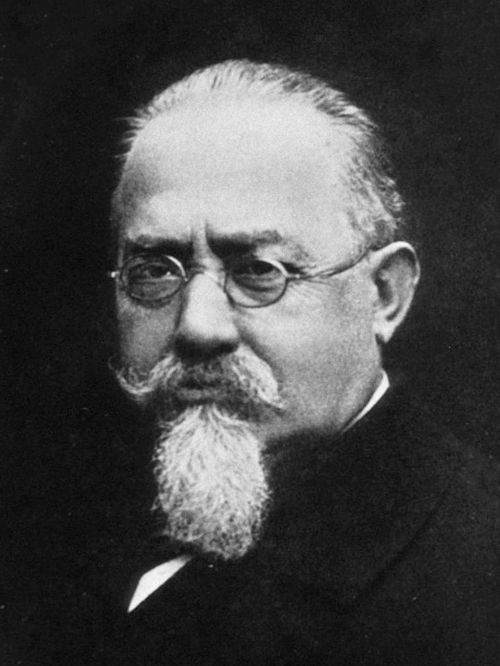
\includegraphics[keepaspectratio]{images/lombroso.JPG}}

}

\caption{Imagen de Lombroso (Fuente: Wikipedia)}

\end{figure}%

Lombroso era un médico que había trabajado para el ejercito italiano y
había estado al mando de varios asilos mentales. Estaba comprometido con
el desarrollo de una ciencia sobre el comportamiento criminal y estaba
influenciado por el \emph{positivismo científico}, un movimiento
filosófico que aspiraba al análisis racional y que ponía su fe en el
progreso científico. El positivismo proponúa un enfoque empírico e
inductivo para comprender las leyes de la naturaleza y del
comportamiento humano. Era un método consistente en el análisis de datos
obtenidos por medio de la observación científica.

En su libro estudio la fisionomía de 832 delincuentes vivos, 390 de los
cuales fueron comparados con 868 soldados italianos y 90 ``lunáticos'' y
fue a partir de estas comparaciones que desarrollo sus conclusiones.
Para Lombroso había varios tipos de delincuentes, uno de los cuales era
el delincuente innato. Seres que no han seguido la evolución genética
natural que el resto de los humanos, lo cual se manifestaba en:
múltiples deficiencias degenerativas de tipo físico (orejas grandes,
brazos demasiado largos, narices torcidas, etc.); peculiaridades
sensoriales y funcionales (p.ej., menos sensibilidad al dolor y al
contacto); una falta de sentido de la moralidad (p.ej, incapacidad de
arrepentimiento); así como otras manifestaciones (lenguaje criminal, uso
extensivo de tatuajes, etc.).

La teoría de la degeneración, según la cual determinadas pautas de
comportamiento problemático como la delincuencia o el alcoholismo, eran
el resultado de saltos hacia atras en el proceso de la evolución humana
que podía transmitirse genéticamente se convirtió en otras de las
obsesiones de los científicos del período (Rafter 2011).

En Estados Unidos fue particularmente influyente el estudio de la
familia ``Jukes'' realizado por Richard Dugdale (1877), que usaba cartas
genealogicas y la historia criminal y social de esta familia, para
intentar demostrar la transmisión hereditaria de este tipo de pautas de
comportamiento problemático y avanzar la idea de un determinismo
biólogico más duro.

Estas ideas perduraron hasta bien entrado el siglo XX. El antropologo
Earnest Hooton publicaba en 1939 Crime and the Man y The American
Criminal conluyendo que los delincuentes eran biológicamente inferiores
y que determinados grupos etnoraciales eran mas comunes en particulares
formas delictivas. Para hacer más atractiva sus ideas, Hooton tomó la
decisión, sin duda desaconsejable, de ilustrar su texto con un estilo de
un mal gusto asombroso.

\begin{figure}[H]

{\centering \pandocbounded{
\includegraphics[keepaspectratio]{images/hooton3.gif}}

}

\caption{Diferencias etnoraciales en delitos sexuales segun Hooton}

\end{figure}%

Hoy en día estas ideas nos parecen lo que son, ridículas. Aunque estos
autores proponían el desarrollo de conclusiones sobre la base de la
observación empírica, sus métodos y presuposiciones eran, contemplados
con nuestro conocimiento actual, burdos y primitivos. Las implicaciones
políticas de estas ideas fueron tremendamente problemáticas. Dieron
lugar al movimieno eugenésico que propuso el internamiento,
esterilización y otro tipo de medidas orientadas a prevenir la
reproducción biológica de estas personas que se consideraban
contaminadas (Rafter 1997). Más tarde en Europa el sustrato de estas
ideas alimentó la barbarie nazi y su ``solución final'' para proteger la
``limpieza de la raza'' (Rafter 2008).

La creciente popularidad de explicaciones sociales de la delincuencia
durante el siglo XX sirvió para que estas perspectivas fueran perdiendo
fuelle. Lo patológico se desplazó del individuo a lo social. Los
sociologos, asociados entre otras a la llamada Escuela de Chigaco y que
de forma más dedicada empezaron a estudiar el delito a partir de la
década de 1930, rechazaban la lógica de los darwinistas sociales de que
los pobres, y los delincuentes entre ellos, eran biológicamente
inferiores y habían caído al último peldaño de la sociedad por ser de
menor valía. Los progresistas preferían una interpretación más
optimista: los pobres eran empujados por su entorno ---no nacían así---
a una vida de delincuencia.

\subsection{``Todos lo hacen''}\label{todos-lo-hacen}

La década de los 1940 supuso un antes y un después en la
conceptualización de los delincuentes. Durante este período se empezó a
experimentar con el método de las encuestas de autoinforme (Kivivuori
2011). Estas encuestas, inicialmente empleadas solamente con muestras de
menores en ambitos educativos, preguntaban a los participantes en las
mismas sobre su participacion en actividades desviadas y delictivas.
Aunque inicialmente se preguntaba sobre comportamientos infractores de
caracter casi trivial a lo largo de los ultimos 75 años se pasó a usar
estas encuestas para estudiar comportamientos delictivos más serios con
muestras también de mayor edad.

Mientras que durante el siglo XIX el delito se conceptualizaba como una
aberración, estas encuestas comenzaron a generar la idea de que ``todo
el mundo lo hace'', que el comportamiento delictivo es mucho más común
de lo que se pensaba y que muchas de las diferencias de clase, raza, y
otros marcadores individuales entre delincuentes y no delincuentes
desaparecían o se diluían mucho cuando en vez de comparar penados y no
penados comparabamos personas que decían cometer infracciones en estas
encuestas con quienes no las confesaban. ¿Cómo seguir manteniendo la
idea de los delincuentes como seres diferenciados y especiales si el
comportamiento delictivo es tan relativamente común y presente en todos
los grupos sociales? ¿Quizás lo que tenemos que preguntarnos es porque
dados niveles similares de participación delictiva en distintos grupos
sociales es porque los penados, aquellos que perseguimos policial y
penalmente, proceden particularmente de determinados grupos sociales y
no de otros?

En 1940-41 fue el sociologo norteamericano Austin Porterfield quien
conducía el pionero estudio que lo cambió todo. Publicado en 1943 en un
articulo titulado \emph{Delinquency and its outcome in Court and
College} y posteriormente en su libro de 1946 \emph{Youth in Trouble:
Studies in Delinquency and Despair}.

\begin{figure}[H]

{\centering \pandocbounded{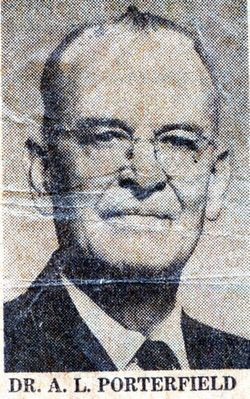
\includegraphics[keepaspectratio]{images/porterfield.jpeg}}

}

\caption{Profesor Austin L. Porterfield (1896-1979)}

\end{figure}%

Porterfield fue uno de los primeros autores en demostrar en detalle como
el control social conforma la poblacion de delincuentes registrados y de
que forma las estadisticas criminales son construcciones sociales. Su
estudio comparando los delincuentes penados y los estudiantes
universitarios mostraba una prevalencia parecida en el tipo de
infracciones que medía. Su conclusión era que:

\begin{quote}
``Los delincuentes no son una subespecie del homo sapiens\ldots. La
conducta antisocial de estudiantes y penados sugiere los mismos anhelos
fundamentales: nuevas experiencias, aventura, estimulación, retos,
reconocimiento, respuestas personales - en resumen, el completo espectro
de emociones humanas'' (Porterfield 1946, 45)
\end{quote}

Desde entonces cientos de estudios han usado encuesta de autoinforme,
algunas con muestras nacionales y como parte de esfuerzos comparativos a
nivel internacional, como el \emph{International Self-Report Study}, en
el que en varias ocasiones ha participado España como vimos en capítulos
anteriores.

Quizás una de las encuestas de este tipo que de forma más minuciosa, y
con una muestra representativa nacional, aspiró a medir de forma muy
detallada delincuencia de caracter no solamente leve sino tambien seria
a efectos de realizar estimaciones rigurosas de caracter nacional fue la
\emph{Offending Crime and Justice Survey} realizada por el británico
\emph{Home Office}.

\begin{figure}[H]

{\centering \pandocbounded{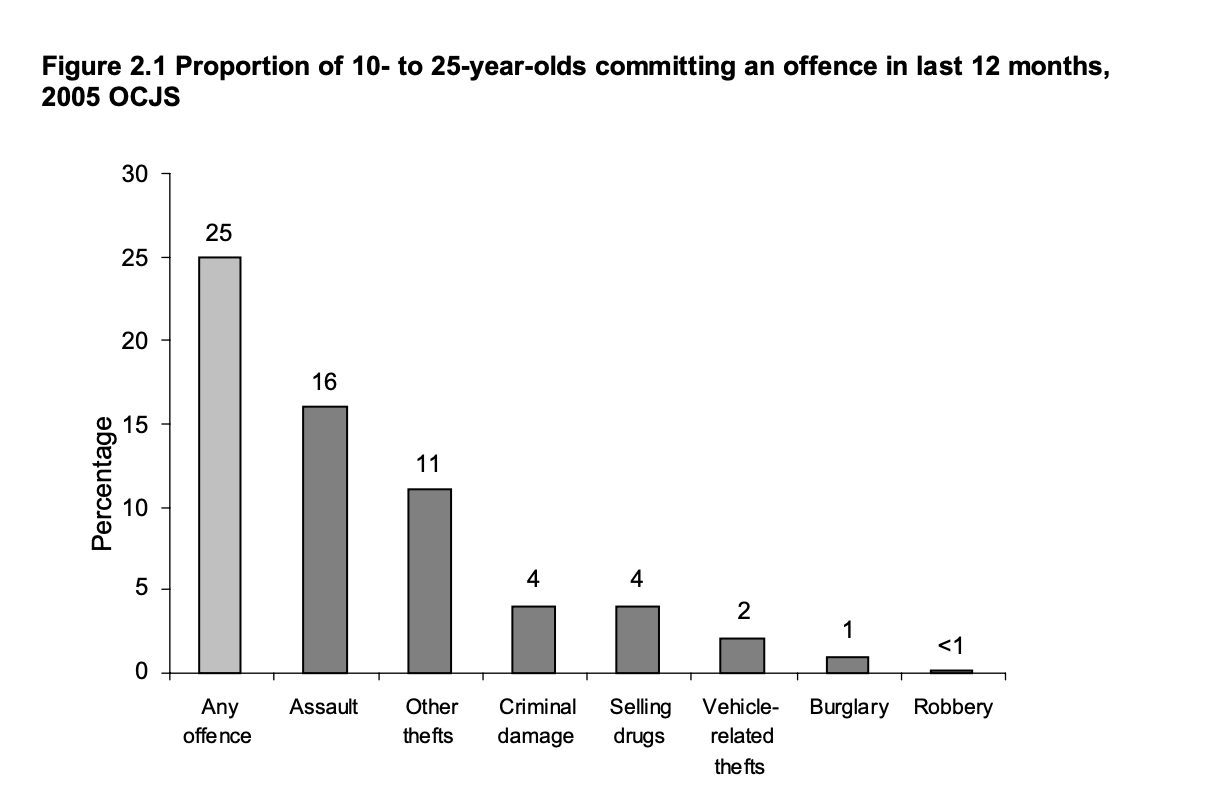
\includegraphics[keepaspectratio]{images/ocjs.png}}

}

\caption{Delincuencia confesada en la Offending Crime and Justice Survey
(Fuente: Wilson et al.~(2006))}

\end{figure}%

Según este estudio un cuarto de la población de Inglaterra y Gáles con
una edad comprendida entre los 10 y 25 años había cometido un delito en
los previos 12 meses. La mitad de estas infracciones eran según los
autores ``delitos serios'' (lesiones, robos de vehículos, robos en
viviendas, venta de drogas de clase A o robos con violencia) (Wilson,
Sharp, y Patterson 2006). Este tipo de datos seriamente cuestiona la
idea de que podemos distinguir claramente entre delincuentes y no
delincuentes.

A nivel teórico y conceptual, la criminología siguió profundizando en
los problemas de la imagen del hombre criminal planteado por el
positivismo criminológico. Así, David Matza en su influyente
\emph{Delinquency and Drift} cuestionaba la idea positivista del
delincuente como esencialmente diferente o patológico. Para Matza (1964)
las teorías positivistas predecían más delincuencia de la que ocurre por
varias razones:

\begin{itemize}
\item
  Los delincuentes no delinquen de forma persistente sino de forma
  episódica, la mayor parte del tiempo se la pasan en actividades
  convencionales
\item
  Los delincuentes llega un momento en que experimentan ``reforma de
  maduración'', dejan de delinquir una vez llegada cierta edad
\item
  La escuela positivista negaba la capacidad de agencia de los
  delincuentes, mostrándolos como individuos sujetos a fuerzas
  totalmente fuera de su control
\end{itemize}

\section{Delincuencia a lo largo de la
vida}\label{delincuencia-a-lo-largo-de-la-vida}

\subsection{La curva del delito y la carrera
criminal}\label{la-curva-del-delito-y-la-carrera-criminal}

De la misma forma que durante la década de 1940 el método del
autoinforme revolucionó la criminología, a partir de los años 1970 otra
innovación metodológica vino a condicionar nuestra visión del
delincuente. Durante este período comienzan a sucederse \textbf{estudios
longitudinales} que seguían a muestras o cohortes locales de individuos
durante largos períodos de sus vidas. Estos estudios permitieron
examinar de forma sistemática de qué forma la participación en
actividades delictivas cambia a lo largo del tiempo.

Uno de los más claros correlatos del delito es la edad. Sabemos que
existe una relación curvilínea entre delincuencia y edad. Hirschi y
Gottfredson (1983) lo caracterizaban como un de las pocas observaciones
fácticas en criminología que no es cuestionada por nadie. La curva suele
adoptar la forma ilustrada en la siguente imagen.

\begin{figure}[H]

{\centering \pandocbounded{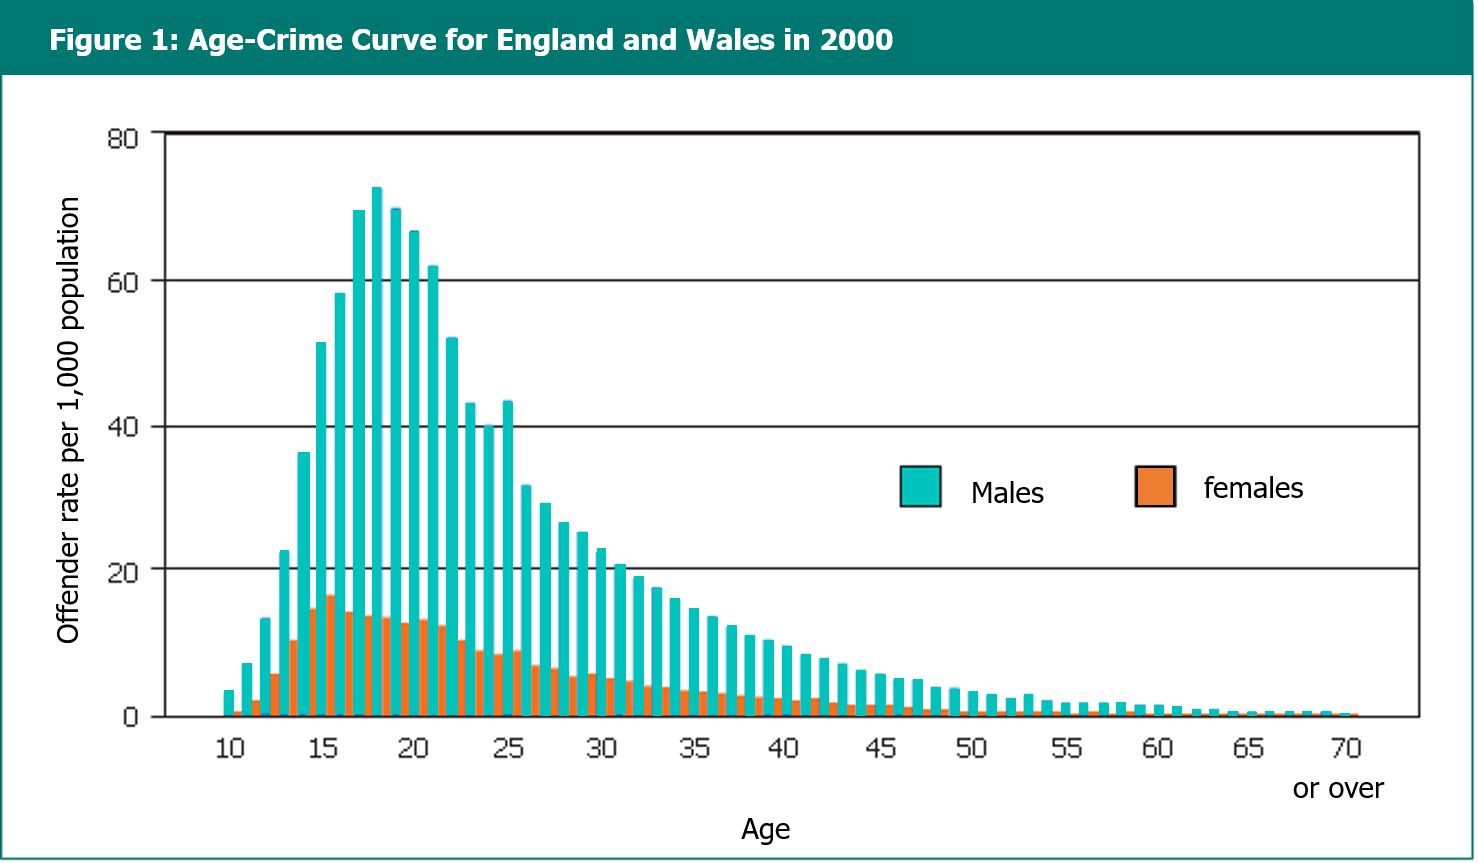
\includegraphics[keepaspectratio]{images/age_crime.png}}

}

\caption{La relación entre edad y delincuencia (Fuente: Her Majesty
Inspectorate of Probation)}

\end{figure}%

La participación en actividades delictivas aumenta durante la
adolescencia, alcanza un pico cerca de la mayoría de edad y, a partir de
ahí, comienza a descencer con el paso del tiempo.

En 1986 se publica un muy influyente informe del \emph{National Research
Council} coordinado por Al Blumstein que consolida el concepto de la
\textbf{carrera criminal} y una serie de ideas básicas ligadas a este
concepto. Una carrera criminal se define como ``la caracterización de la
secuencia longitudinal de delitos cometidos por un individuo'' (National
Research Council 1986, 12). Una carrera criminal está definida por
varios parametros:

\begin{itemize}
\item
  \emph{Participación}: la distinción entre quienes inician una y
  quienes no.
\item
  \emph{Frecuencia}: la tasa delictiva de los delincuentes mientras se
  encuentran en activo. Esto es, el número de delitos cometidos por cada
  delincuente por cada año en que se encuentran activos. Este parametro
  vino a denotarse con la letra griega \emph{lambda}.
\item
  \emph{Seriedad}: la gravedad de los delitos cometidos.
\item
  \emph{Escalada}: la tendencia a cometer delitos más serios.
\item
  \emph{Duración de la carrera}: el período de tiempo que transcurre
  desde que los delincuentes se inician en la comisión de actos
  delictivos y el momento en que dejan de cometer delitos.
\end{itemize}

Estos elementos se pueden ver representados en la figura que incluían en
el primer capítulo de este informe:

\begin{figure}[H]

{\centering \pandocbounded{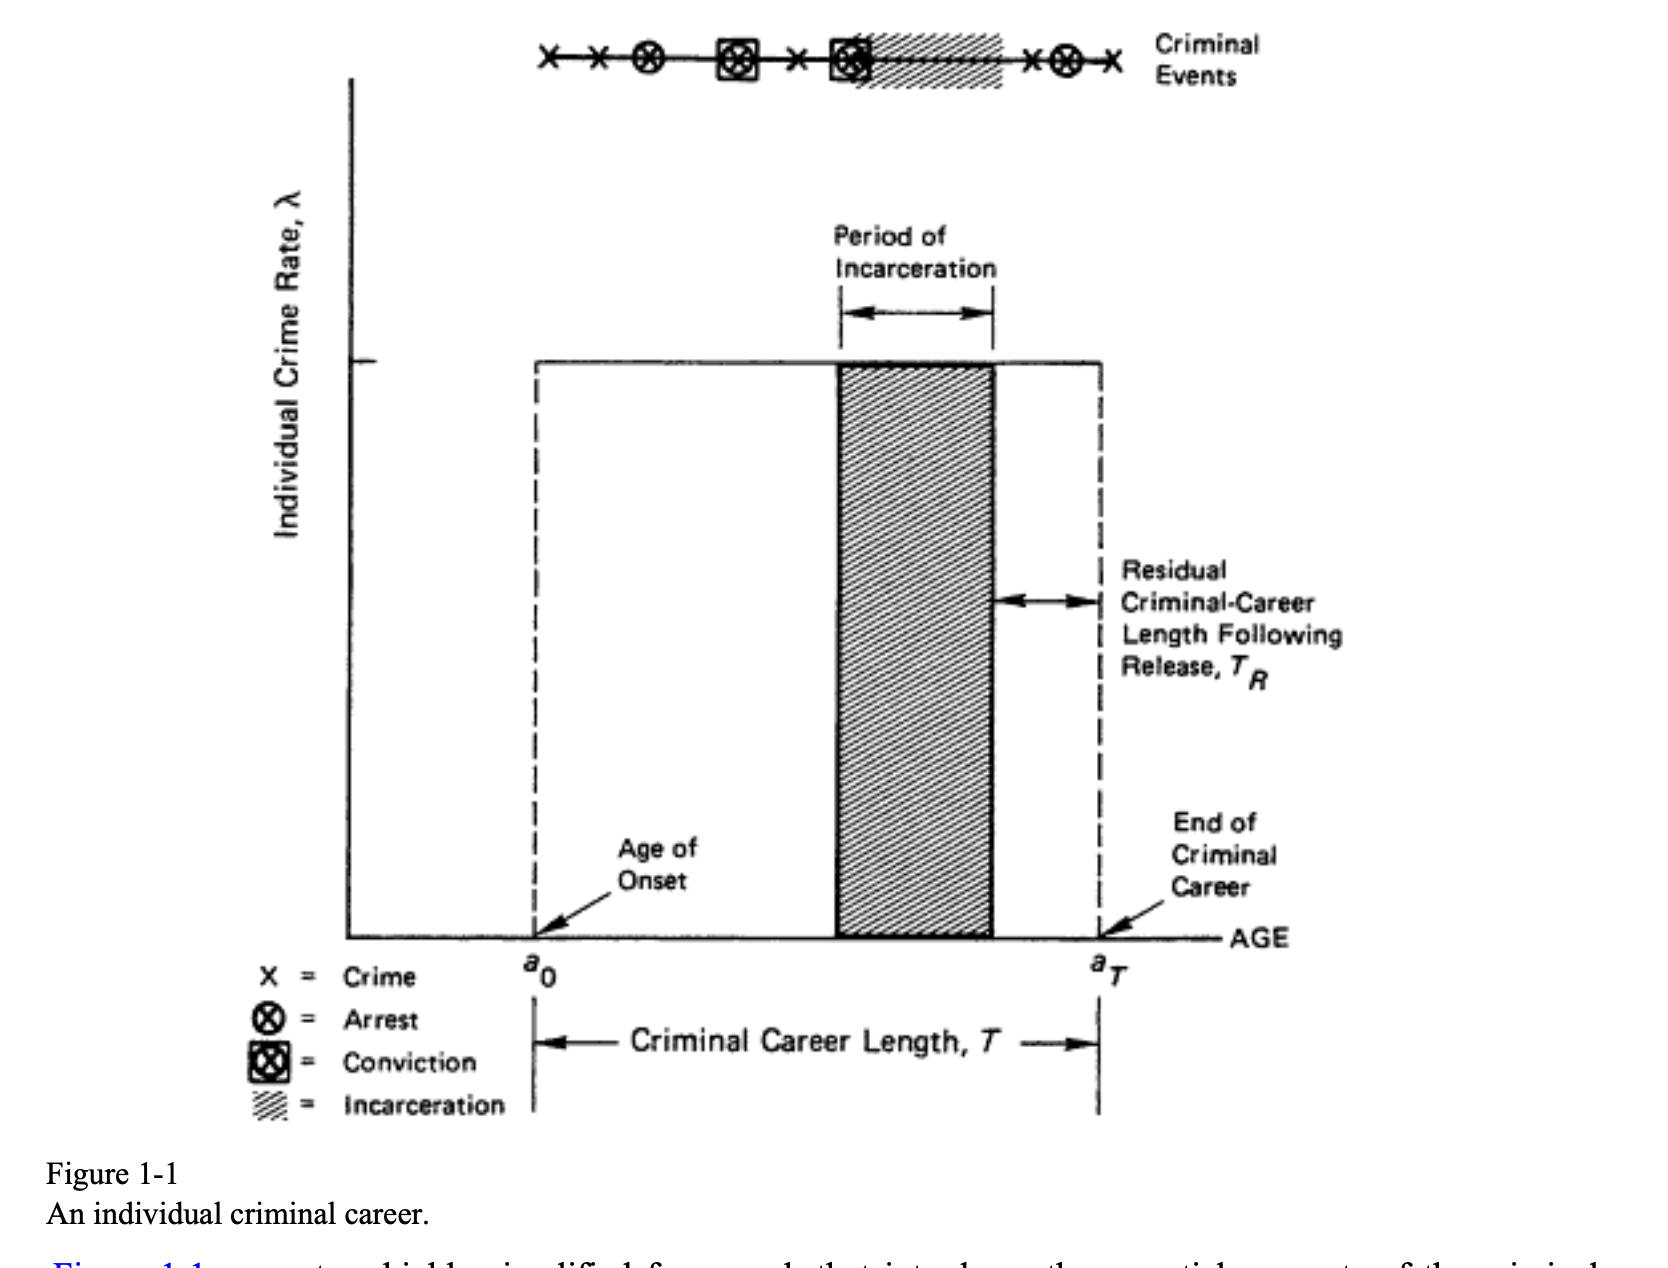
\includegraphics[keepaspectratio]{images/career.png}}

}

\caption{Representación gráfica de una carrera criminal (Fuente:
National Research Council, 1986)}

\end{figure}%

Las carreras criminales tienen un inicio (en inglés ``onset'') y un
momento en el que finalizan. Durante este período en el que se
encuentran activos los delincuentes cometen un número de delitos X, una
minoría de los cuales son detectados y sancionados por el sistema penal
(dando lugar a periodos en los que los delincuentes, si encuentran en
prisión, se encuentran incapacitados para cometer delitos que requieran
su presencia física fuera de la prisión).

Durante años la investigación criminológica se ha esforzado en tratar de
estimar todos estos parametros (edad de iniciación, lambda, duración de
carreras criminales, etc.), siendo una labor arduo compleja.
Evidentemente, estas cantidades varían en función de la persona.

Por lo que aquí respecta, lo importante a subrayar es que este enfoque
supuso un paso determinante a entender la delincuencia como una etapa
transitoria en la vida de las personas que cometen algún delito en su
vida, no como una calidad o condición inmutable de las personas. Tan
relevante es ahora esta relación que:

\begin{quote}
``A los teóricos se les recuerda con frecuencia que sus explicaciones
sobre la de incuencia deben ajustarse a la distribución por edades, y
las teorías se juzgan a menudo por su capacidad para abordar la «reforma
madurativa», la «remisión espontánea» o el efecto del
«envejecimiento».'' (Hirschi y Gottfredson 1983, 553)
\end{quote}

La criminología evolutiva que ha dominado el estudio de los delincuentes
durante las últimas décadas básicamente ha venido a aceptar que
(Steffensmeier, Slepicka, y Schwartz 2025, 241):

\begin{quote}
\begin{itemize}
\item
  El grupo de edad de entre los 15 a 19 es el que exhibe una mayor tasa
  de participación en actividades delictivas.
\item
  La delincuencia entre los adolescentes tiene tasas de prevalencia
  altas, con un porcentaje elevado de los mismos participando en
  actividades delictivas.
\item
  La curva del delito se caracteriza por un rápido aumento y un pico
  temprano, seguido de un rápido descenso inicial y luego un descenso
  gradual.''
\end{itemize}
\end{quote}

\begin{tcolorbox}[enhanced jigsaw, bottomtitle=1mm, toprule=.15mm, colbacktitle=quarto-callout-note-color!10!white, bottomrule=.15mm, leftrule=.75mm, colframe=quarto-callout-note-color-frame, opacitybacktitle=0.6, titlerule=0mm, breakable, colback=white, left=2mm, arc=.35mm, title=\textcolor{quarto-callout-note-color}{\faInfo}\hspace{0.5em}{Nota}, toptitle=1mm, coltitle=black, rightrule=.15mm, opacityback=0]

\textbf{¿Son las premisas de la curva de la edad y el delito
universales}

\end{tcolorbox}

De forma relacionada dentro de la criminología se vino a desarrollar lo
que se llamó el \textbf{paradigma del factor de riesgo}, que tuvo entre
sus más prolíficos defensores al británico David Farrington, que fue
investigador en uno de los primeros y mas famosos estudios
longitudinales de la delincuencia el \emph{Cambridge Study in Delinquent
Development}, un estudio de 411 varones nacidos en Londres en 1953 en
barrios empobrecidos y que fueron seguidos desde que tenían 8/9 años
hasta sus 48.

Este paradigma invitaba a la identificación de factores de riesgo
asociados con el inicio (y otros parámetros como persistencia, escalada,
etc.) de carreras criminales para a continuación proponer métodos de
prevención que sirvan para reducirlos (Farrington 2000, 2).

\begin{quote}
``El paradigma de prevención de factores de riesgo fue importado a la
criminología desde la medicina y la salud pública \ldots{} Este
paradigma se ha utilizado con éxito durante muchos años para combatir
enfermedades como el cáncer y las cardiopatías. Por ejemplo, los
factores de riesgo identificados para las enfermedades cardíacas
incluyen el tabaquismo, una dieta rica en grasas y la falta de
ejercicio. Estos pueden abordarse animando a las personas a dejar de
fumar, a seguir una dieta más saludable y baja en grasas, y a hacer más
ejercicio.''
\end{quote}

Un \textbf{factor de riesgo} es simplemente algo que incremente la
probabilidad de la actividad delictiva, no necesariamente una causa,
sino simplemente un factor que aumenta dicha probabilidad. Este enfoque
condujo a la proliferación de modelos explicativos de la participación
en actividades delictivos de tipo multifactorial. Por ejemplo, para J.
Murray y Farrington (2010) Los factores de riesgo más importantes que
correlacionan con la delincuencia incluyen la impulsividad, un
coeficiente intelectual bajo y un rendimiento escolar bajo, una
supervisión parental deficiente, una disciplina parental punitiva o
errática, una actitud parental fría, el maltrato físico infantil, los
conflictos parentales, las familias desestructuradas, los padres
antisociales, las familias numerosas, los bajos ingresos familiares, los
compañeros antisociales, las escuelas con altas tasas de delincuencia y
los barrios con altos índices de criminalidad.

\subsection{El 6\% crónico, los criminales de carreras y las
trayectorias diferenciales de
delincuencia}\label{el-6-cruxf3nico-los-criminales-de-carreras-y-las-trayectorias-diferenciales-de-delincuencia}

Otro de los primeros estudios longitudinales realizados en Estados
Unidos también tuvo un impacto notable en nuestra imagen de los
delincuentes. El \emph{Delinquency Birth Cohort} fue un estudio liderado
por el criminólogo Marvin Wolfgang que exploró las trayectorias
delictivas de todos los 9945 niños nacidos en 1945 y que vivían en
Filadelfia entre los 10 y los 18 años (Wolfgang, Figlio, y Sellin
(1972)). Una vez establecida la cohorte, los investigadores recopilaron
datos sobre los 3475 delincuentes que habían tenido contactos oficiales
con la policía no relacionados con la seguridad vial entre los 7 y los
18 años de edad. A partir de estos datos oficiales, el estudio estimó
las probabilidades de cometer el primer delito, la reincidencia, el
aumento de la gravedad de los delitos a lo largo del período observado,
la edad de inicio, etc.

\begin{figure}[H]

{\centering \pandocbounded{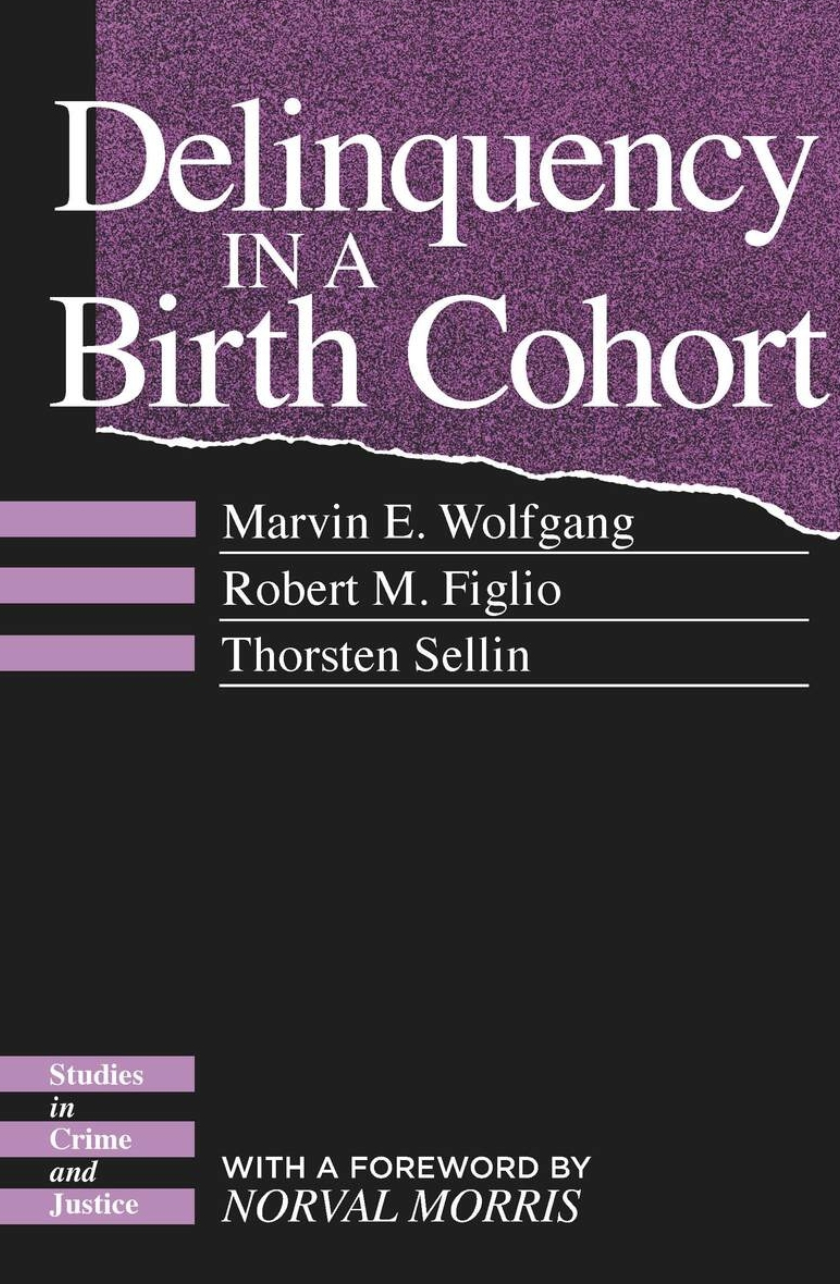
\includegraphics[keepaspectratio]{images/birth_cohort.png}}

}

\caption{Portada de Delinquency in a Birth Cohort}

\end{figure}%

El estudio documentó que había un 35\% de probabilidades de que los
niños hubieran sido arrestados al menos una vez por delitos distintos de
infracciones de tráfico, reiterando las altas tasas de participación
delictiva. Sin embargo, solo el 6 \% de la cohorte eran delincuentes
crónicos (habían sido arrestados al menos cinco veces antes de los 18
años) y este 6\% de delincuentes crónicos eran responsables de más del
50 \% de todos los delitos. Un estudio de una cohorte posterior, de
1958, replicó el primer estudio, excepto que incluyó a mujeres. En el
segundo estudio, el porcentaje de delincuentes crónicos fue del 7,5 \%,
y cometieron el 69 \% de los delitos indexados. Alrededor del 9 \% de
los 13,800 niños del segundo estudio y alrededor del 2 \% de las 14,500
niñas cometieron un delito violento que causó lesiones a una persona.

Los datos de este estudio se vinieron a interpretar como un complemento
al momento ``todos lo hacen'' generados por los primeros estudios de
auto-informe. Aunque era cierto, y así lo demostraba también este
estudio, que el comportamiento infractor es mas común de lo que a
menudos pensamos (el 35\% de los menores en la primera cohorte tenía
algun antecedente policial), la clara detección de un porcentaje menor
de estas cohortes que exhibían una mayor propensión a la reincidencia
tuvo también repercusiones científicas y políticas importantes.

A partir de entonces empezó a hablarse del ``6\% crónico'' para designar
de forma simbólico a ese subconjunto de delincuentes con una particular
propesión hacía la comisión de delitos. Aunque los avances realizados
durante el siglo XX hacían ridículo el pensar que podemos diferenciar a
los delincuentes de los no delincuentes, este tipo de estudios vino a
sugerir de alguna forma que hay un particular perfil de delincuentes con
niveles altos de reincidencia que quizás nos debería preocupar.

Años más tarde la también normeamericana Terrie Moffitt publicó un muy
influyente artículo que trataba de reconciliar los datos que estudios
longitudinales posteriores habían ido generando sobre trayectorias
delictivas. En un muy influyente artículo publicado en 1993 y titulado
\emph{Adolescence-Limited and Life-Course-Persistent Antisocial
Behavior: A Developmental Taxonomy} la profesora Moffitt proponía la
existencia de dos tipos ideales de trayectorias delictivas, \textbf{la
trayectoria limitada a la adolescencia} y \textbf{la trayectoria
antisocial persistente a lo largo de la vida}.

\begin{figure}[H]

{\centering \pandocbounded{
\includegraphics[keepaspectratio]{images/moffitt.jpeg}}

}

\caption{Imagen the Terrie Moffitt}

\end{figure}%

Para Moffitt (1993), el comportamiento antisocial es muy común en la
adolescencia. Según ella habría un subtipo de personas que cometen
delitos que inician sus breves carreras criminales durante la
adolescencia y la culminan al transitar a la vida adulta. Este grupo
sería el que mostraría una trayectoria delictiva limitada a la
adolescencia. Para Moffitt (1993) sobre todo los deseos de aventura e
independencia y los cambios hormonales y biológicos durante este
período, combinado con las malas influencias de los iguales serían los
factores clave para entender el comportamiento antisocial de las
personas en esta trayectoria.

\begin{quote}
``Presento tres hipótesis etiológicas. El comportamiento antisocial
limitado a la adolescencia está motivado por la brecha entre la madurez
biológica y la madurez social, se aprende de modelos antisociales que
son fácilmente imitables y se mantiene de acuerdo con los principios de
refuerzo de la teoría del aprendizaje.'' (Moffitt 1993, 685)
\end{quote}

Para Moffitt (1993) el comportamiento delictivo de este subgrupo puede
considerarse comportamiento social adaptativo, no sería en su opinión
posible conceptualizarlo como comportamiento patológico. Generalmente,
personas en esta trayectoria desisten de la delincuencia al transitar a
la vida adulta.

\begin{figure}[H]

{\centering \pandocbounded{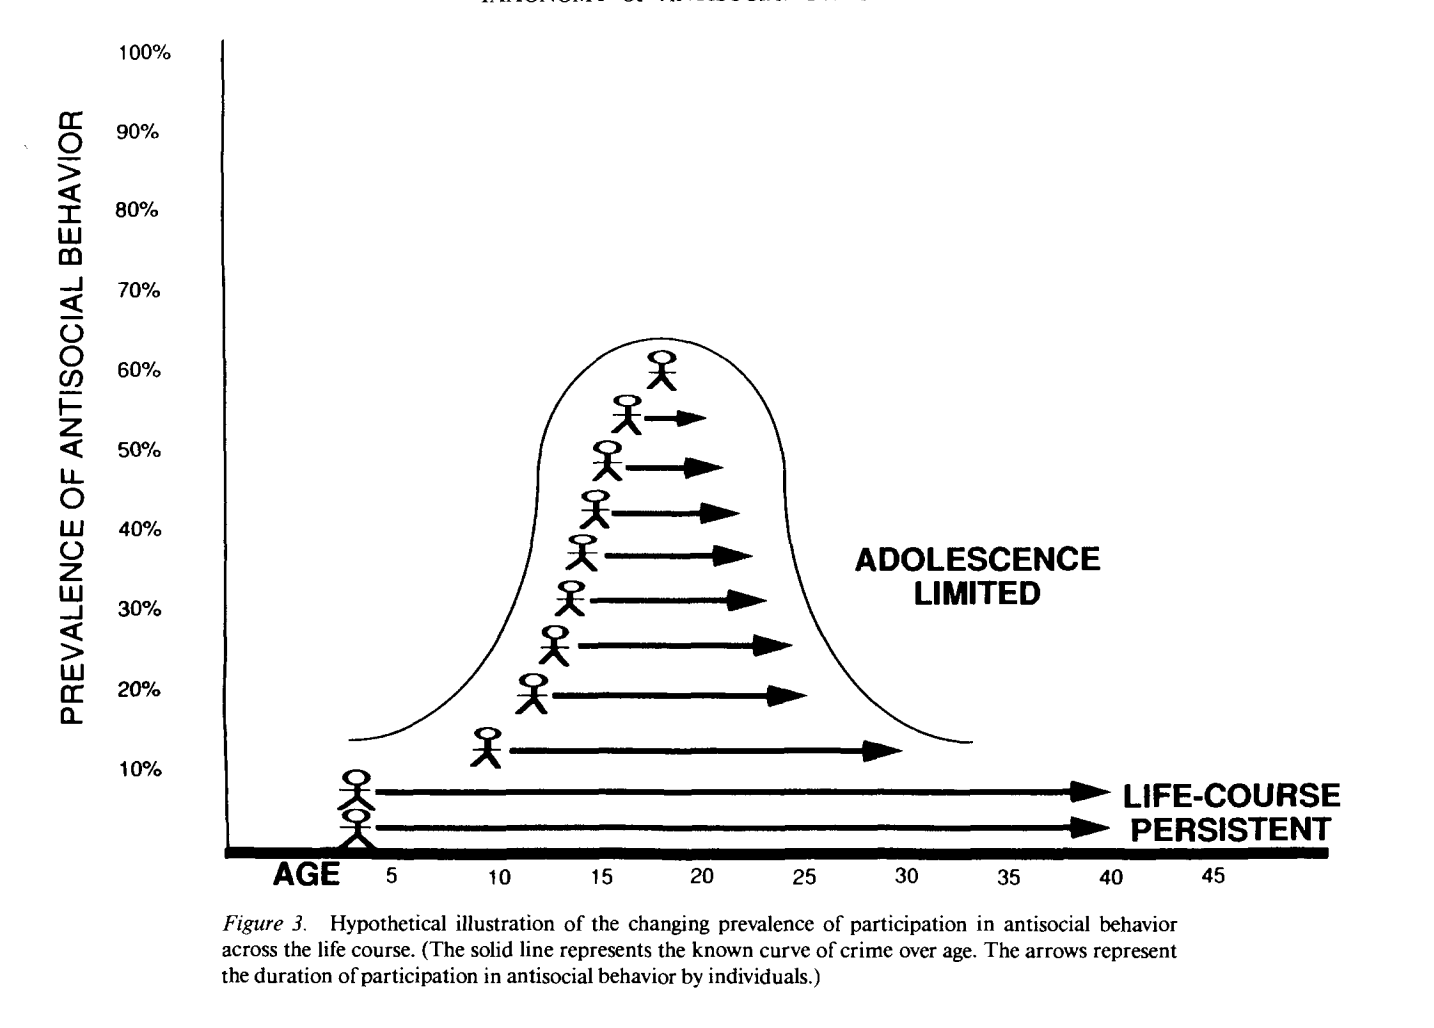
\includegraphics[keepaspectratio]{images/trajectories.png}}

}

\caption{Las dos trayectorias delictivias teorizadas por Moffitt}

\end{figure}%

Por el otro lado tendríamos el subgrupo que Moffitt define como
antisociales persistentes a lo largo de la vida. Un perfil que sería lo
que Wolfgang, Figlio, y Sellin (1972) había identificado como el 6\%
crónico. Este subgrupo de delincuentes, según Moffitt (1993), tendría
una edad de inicio en la delincuencia y el comportamiento problemático
más temprano, ya se manifestaría durante la infancia, y el mismo se
prolongaría en el tiempo bien pasado el tránsito a la vida adulta. Este
grupo vendría caracterizado por la continuidad del comportamiento
delictivo:

\begin{quote}
``A lo largo del tiempo estos individuos muestran manifestaciones
cambiantes de su comportamiento antisocial: mordiscos y golpes a la edad
de 4 años, hurtos en tiendas y faltar a clase a los 10, vender drogas y
robar coches a los 16, atracos y violaciones a los 22, fraudes y abuso
infantil a los 30; la disposición subyacente permanece, pero su
expresión cambia forma en la medida en que nuevas oportunidades se
presentan a lo largo de su desarrollo vital'' (Moffitt 1993, 679).
\end{quote}

El inicio temprano en la delincuencia de este subgrupo para Moffitt
(1993) resulta de la interacción en estos menores de vulnerabilidades
neuropsicológicas con el haber crecido en ambientes criminógenos. Es la
presencia en la edad temprana de estos individuos de estos factores que
pueden servirnos para entender el prematuro inicio de su comportamiento
antisocial.

El trabajo de Moffit ha tenido un impacto muy notable en la criminología
contemporanea. El artículo que hemos mencionado ha sido citado más de
18,000 veces por otros estudios científicos, que es una auténtica
barbaridad. Numerosos investigadores han tratado de validar con datos
procedentes de estudios longitudinales la existencia de estos tipos
ideales identificados por Moffit.

Las investigaciones longitudinales y transnacionales encuentran
sistemáticamente múltiples y distintas trayectorias de desarrollo de la
delincuencia. La mayoría de los estudios identifican al menos entre tres
y cinco grupos (aunque algunos identifican más), tales como los no
delincuentes, los delincuentes crónicos de bajo nivel, los delincuentes
adolescentes y los delincuentes crónicos de alto nivel.

A pesar de la amplia coherencia, el número exacto y la forma de las
trayectorias pueden variar debido a (Egglestone, Laub, y Sampson 2004):

\begin{itemize}
\item
  Las opciones de modelización estadística.
\item
  Las características de la muestra (por ejemplo, población general
  frente a muestras de alto riesgo o delincuentes).
\item
  Las definiciones operativas de delincuencia y cronicidad.
\item
  La duración del seguimiento, de que edad a que edad se sigue a los
  participantes en el estudio, influye en los patrones de trayectoria.
\item
  Otro problema importante es que la información sobre encarcelamiento y
  mortalidad se ha descuidado en investigaciones anteriores.
\end{itemize}

Una revisión sistemática de 55 estudios prospectivos longitudinales
reveló que la prevalencia de los delincuentes crónicos varía
considerablemente, pero la mayoría de los estudios indican que los
delincuentes crónicos constituyen una pequeña minoría, generalmente
entre el 1\% y el 10\% de la población estudiada, con muchas
estimaciones cercanas al 5\% (Jolliffe et~al. 2017). Este grupo es
sistemáticamente mucho más pequeño que los grupos de delincuentes
limitados a la adolescencia u otros grupos de delincuentes. En muestras
de la población general, la prevalencia de LCP suele ser del 1-5\%,
mientras que en muestras de alto riesgo o correccionales, la proporción
puede ser mayor, superando en ocasiones el 10\%. El género y el contexto
son importantes: la prevalencia del grupo de delincuentes crónicos es
menor entre las mujeres y mayor en los grupos desfavorecidos o de alto
riesgo.

Conviene destacar que algunos autores son críticos de este tipo de
trabajo. Los críticos sostienen que los modelos de trayectoria de
desarrollo suelen presuponer la existencia de grupos de delincuentes
diferenciados (Sampson y Laub 2005). Las técnicas de modelado
estadístico empleado \emph{asumen} que hay grupos diferenciados y, por
tanto, van a encontrar grupos diferenciados. ¿Pero son estos grupos
teóricamente tan relevantes como se supone?

Los modelos de desarrollo que identifican estas trayectorias como
determinantes pueden subestimar el papel de la agencia humana, al tratar
el comportamiento delictivo como algo determinado en gran medida por
factores de la primera infancia o la pertenencia a una trayectoria
concreta, en lugar de reconocer las decisiones continuas y deliberadas
que los individuos toman a lo largo de su vida (\textbf{Sampson\_03?}).

Los modelos de trayectoria basados en grupos son valiosos para
visualizar y describir datos (Brame, Paternoster, y Piquero 2012), pero
los críticos advierten que pueden no proporcionar un gran poder
explicativo o predictivo con respecto a las causas del comportamiento
delictivo.

Los factores de riesgo en la infancia y los pronósticos tempranos, que
Moffit señalaba como relevantes para identificar y predecir a los
delincuentes crónicos, a menudo no explican adecuadamente los patrones
delictivos a largo plazo (\textbf{Sampson\_03?}; McCuish, Lussier, y
Corrado 2016). Según estos autores es relativamente facil a posteriori
identificar trayectorias delictivas, cuando tienes datos de
participación delictiva a lo largo de la vida, pero mucho más dificil
hacerlo de forma prospectiva, esto es, identificar que trayectoria una
persona seguirá sobre la base de lo que sabemos sobre ella antes de que
vayan haciendose mayores. Incluso entre los grupos de alto riesgo, la
mayoría de las personas acaban abandonando la delincuencia, lo que pone
en tela de juicio la noción de delincuentes estables y persistentes a lo
largo de toda su vida (\textbf{Sampson\_03?}).

En resumen, los autores críticos destacan que las trayectorias de
desarrollo de la delincuencia pueden simplificar en exceso procesos
complejos y dinámicos, son sensibles a las elecciones metodológicas y, a
menudo, no tienen en cuenta la acción humana y la interacción con el
entorno. Estas críticas exigen enfoques más matizados, integradores y
flexibles para comprender el comportamiento delictivo a lo largo de la
vida.

\subsection{Desistimiento o
desistencia}\label{desistimiento-o-desistencia}

Al margen del debate que existe en torno a las trayectorias delictivas,
lo cierto es que generalmente lo normal es que las personas que
participan en actividades delictivas acaban desistiendo de la
delincuencia.

La desistencia, o desestimiento, se refiere al proceso por el cual las
personas dejan de participar en conductas delictivas. Los distintos
autores que han investigado la desistencia reconocen ampliamente cque
estamos hablando de un proceso más que de un evento único, que a menudo
implica retrocesos y recaídas antes de lograr una abstinencia sostenida
de la delincuencia. En ese sentido, la desistencia se distingue de la
mera terminación (el punto en el que cesa la delincuencia); ya que
abarcaría los cambios subyacentes que conducen a la abstinencia a largo
plazo.

A lo largo del tiempo ha habido distintas explicaciones teóricas del
proceso del desestimiento. Inicialmente había dos modelos contrapuestos,
uno que ponía el énfasis en circunstancias externas al delincuente
(oportunidades vitales, el desarrollo de nuevos lazos sociales, etc.)
defendida inicialmente por (\textbf{Sampson\_95?}), frente a otro modelo
que ponía el acento en lo subjetivo, en los procesos internos de
transformación cognitiva que tenían que abordar los delincuentes y que
fue inicialmente defendido por Maruna (2001). Hoy se suele reconocer que
ambos elementos son importantes y se suele admitir que hay una serie de
factores que condicionan los procesos de desistencia, incluyendo:

\begin{itemize}
\item
  Vínculos sociales y acontecimientos vitales: Un empleo estable,
  relaciones de apoyo (especialmente el matrimonio y la familia) y
  vínculos sociales positivos.
\item
  Identidad y cambio cognitivo: Los cambios en la identidad propia, el
  aumento de la capacidad de acción y el cambio intencional. Los
  delincuentes que desarrollan una identidad «prosocial» y creen en su
  capacidad de cambiar son más propensos a desistir.
\item
  Factores estructurales y contextuales: Las estructuras sociales más
  amplias (por ejemplo, las oportunidades de empleo, la vivienda, el
  estigma) y los entornos políticos pueden facilitar o dificultar la
  desistencia.
\item
  Procesos emocionales y psicológicos: El equilibrio emocional, la
  esperanza y la capacidad de gestionar la angustia se consideran
  importantes para mantener la desistencia.
\end{itemize}

Se entiende que los cambios de identidad y las estructuras sociales
interactúan dinámicamente en el proceso de desistimiento delictivo,
influyéndose y reforzándose mutuamente. Desarrollar una identidad
prosocial ---verse a uno mismo como una persona ``buena'' o que no
comete delitos--- puede ser un catalizador para dejar de delinquir. Este
cambio suele estar motivado o reforzado por experiencias sociales, como
las relaciones de apoyo, el empleo o la participación en la comunidad.
Las estructuras sociales ---incluidas la familia, las redes de
compañeros, las oportunidades laborales y las actitudes sociales en
general--- pueden facilitar o dificultar la transformación de la
identidad. Los vínculos sociales de apoyo (por ejemplo, con los padres,
la pareja o compañeros prosociales) y el acceso a oportunidades
legítimas ayudan a las personas a mantener nuevas identidades y evitar
recaídas, mientras que las desventajas estructurales (por ejemplo, el
estigma, la falta de empleo, la exclusión de los grupos sociales) pueden
socavar estos esfuerzos. Por tanto, los cambios de identidad y las
estructuras sociales se refuerzan mutuamente. Por ejemplo, el nuevo
concepto que una persona tiene de sí misma puede motivarla a buscar
relaciones y oportunidades prosociales, mientras que la
retroalimentación social positiva y la aceptación consolidan aún más la
nueva identidad. Por el contrario, las barreras estructurales
persistentes o los entornos sociales negativos pueden perturbar o
revertir el cambio de identidad, lo que conduce a la reincidencia.

En resumen, la desistencia delictiva se entiende mejor como un proceso
dinámico y continuo, moldeado tanto por transformaciones internas
(identidad, agencia) como por apoyos externos (relaciones, estructuras
sociales). No existe un único camino y los reveses son comunes, pero los
vínculos sociales positivos y un cambio en la identidad propia están
sistemáticamente relacionados con una desistencia exitosa.

\section{Los ``psicópatas'' y el desorden de personalidad
antisocial}\label{los-psicuxf3patas-y-el-desorden-de-personalidad-antisocial}

Existe una fascinación cultural por la figura de los psicópatas. En la
criminología española, Vicente Garrido, profesor de psicología de la
Universidad de Valencia que juegó un papel clave en la
institucionalización y desarrollo científico de la disciplina en nuestro
país, ha escrito de forma abundante sobre el tema, en ocasiones en
formatos dirigidos a una audiencia general, no solo escritos, por tanto,
para académicos (Garrido 2000b, 2000a, 2000c, 2024). Siguiendo los
títulos de sus libros los psicópatas serían los delincuentes más
peligrosos y sus formas camaleónicas haría que fueran dificiles de
detectar en distintos entornos.

\begin{figure}[H]

{\centering \pandocbounded{
\includegraphics[keepaspectratio]{images/garridopsicopatas.webp}}

}

\caption{Vicente Garrido y una de sus libros sobre el tema}

\end{figure}%

Para el psicólogo canadiense Robert D. Hare (1993, xi), la figura que
más ha hecho para popularizar y desarrollar este concepto:

\begin{quote}
``Los psicópatas son depredadores sociales que seducen, manipulan y se
abren camino sin piedad por la vida, dejando tras de sí un rastro de
corazones rotos, expectativas frustradas y carteras vacías. Carecen por
completo de conciencia y de sentimientos hacia los demás, toman
egoístamente lo que quieren y hacen lo que les place, violando las
normas y expectativas sociales sin el más mínimo sentimiento de culpa o
arrepentimiento.''
\end{quote}

La psicopatía es un constructo clínico y forense que suele
diagnosticarse usando una escala desarrollada por el mencionado Robert
Hare. Este autor desarrolló originalmente la PCL (\emph{Psychopathy
CheckList} o lista de verificación o comprobación de psicopatías) y la
PCL-R (\emph{Psychopathy CheckList Revised} o lista revisada de
verificación o comprobación de psicopatías).

\begin{quote}
``La PCL-R es una escala de valoración clínica que utiliza una
entrevista semiestructurada, información del historial clínico y
criterios de puntuación específicos para valorar cada uno de los 20
ítems en una escala de 3 puntos (0, 1, 2) según el grado en que se
aplica a un individuo determinado. Como se describe a continuación
(sección «En busca de la estructura de la psicopatía»; figura 1), 18 de
los ítems forman cuatro factores o dimensiones: Interpersonal (encanto
superficial/labia, sentido grandioso de la autoestima, mentira
patológica, engaño/manipulación); Afectivo (falta de remordimiento o
culpa, afectividad superficial, insensibilidad/falta de empatía,
incapacidad para aceptar la responsabilidad de las acciones); Estilo de
vida (necesidad de estimulación/propensión al aburrimiento, estilo de
vida parasitario, falta de objetivos realistas a largo plazo,
impulsividad, irresponsabilidad); y Antisocial (control deficiente del
comportamiento, problemas de conducta tempranos, delincuencia juvenil,
revocación de la libertad condicional, versatilidad delictiva). Otros
dos elementos (conducta sexual promiscua, muchas relaciones a corto
plazo) no se incluyen en ningún factor, pero contribuyen a la puntuación
total del PCL-R. Las dimensiones interpersonal/afectiva y estilo de
vida/antisocial comprenden, respectivamente, los factores 1 y 2 del
PCL-R (véase la figura 2) descritos por Hare (2003). Las puntuaciones
totales del PCL-R pueden variar de 0 a 40 y reflejan el grado en que el
individuo se ajusta al prototipo de psicópata. Para fines de
investigación y «diagnóstico», se suele utilizar una puntuación de corte
de 30 para la psicopatía.'' (R. Hare y Neumann 2008, 218-19)
\end{quote}

\begin{figure}[H]

{\centering \pandocbounded{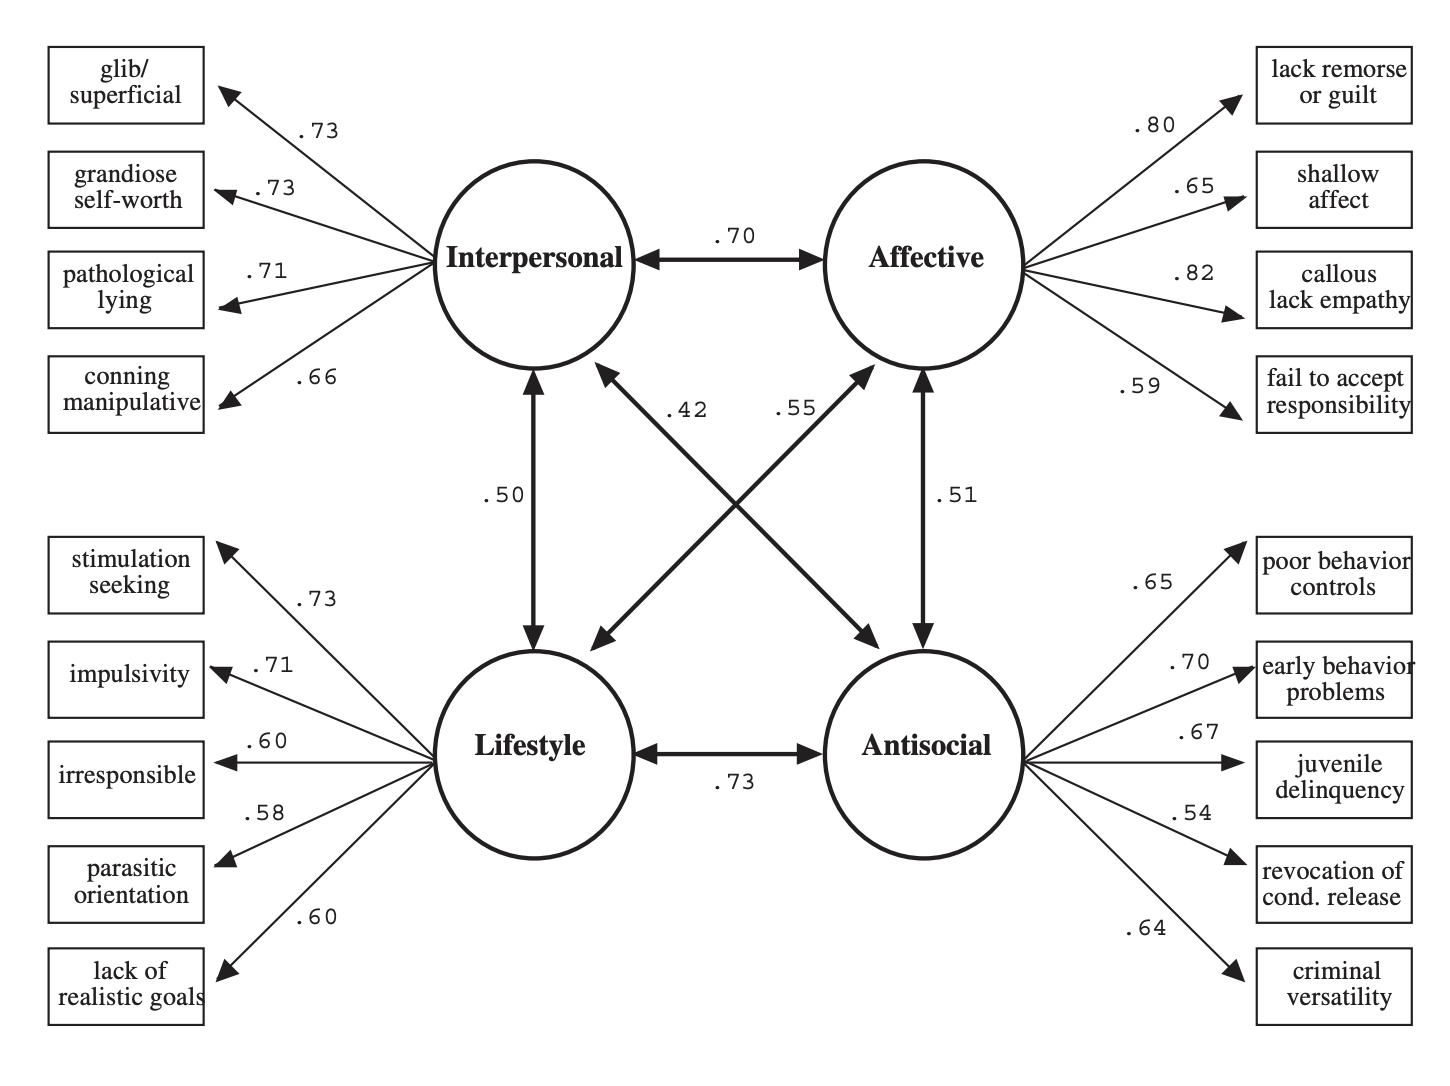
\includegraphics[keepaspectratio]{images/hare.png}}

}

\caption{Estructura factorial de los componentes de la PCL-R}

\end{figure}%

Por tanto, el psicópata se caracterizaría por ser ``una persona
emocionalmente fria, manipuladora, que no tiene sentimientos de culpa o
conciencia, y que es capaz de actuar con gran impulsividad y temeridad,
pero también siguiendo de forma maquiavélica un plan preconcebido''
(Redondo y Garrido 2023, 445). Redondo y Garrido (2023) destacan como
aunque Hare siempre ha defendido que este es un constructo muy solido,
quizás habría que considerar la psicopatía más como un espectro, que se
puede manifestar en distintos grados y de forma diversa, según la
persona.

La psicopatía, como tal, no está reconocida como trastorno por parte de
las clasificiaciones oficiales de psicopatología que se emplean a nivel
internacional. Hay dos instrumentos que se manejan como listados
oficiales de psicopatologías:

\begin{itemize}
\item
  El *Manual diagnóstico y estadístico de los trastornos mentales''.
  Generalmente conocido por su abreviación en inglés, DSM, y que se
  encuentra ahora en su quinta edición, de ahí que se le suela llamar
  DSM-5. Este manual fue desarrollado y ha sido actualizado de forma
  periódica por la Asociacón Americana de Psiquiatría.
\item
  La \emph{Clasificación internacional de las enfermedades}, o
  abreviando ICD-10, que es publicada por la Organización Mundial de la
  Salud y que se encuentra en su décima edición.
\end{itemize}

Ninguno de estos listados oficiales incluye la psicopatía como tal,
aunque es cierto que ambos recogen trastornos que tienen un cierto
solapamiento con la psicopatía. El DSM-5 hace referencia al
\textbf{trastorno antisocial de la personalidad} y el ICD-10 menciona el
\textbf{trastorno disocial de la personalidad}. En ambos casos, y a
diferencia del concepto de psicopatía se pone un mayor énfasis en el
componente antisocial del comportamiento para poder diagnosticas estos
trastornos.

Según el DSM-5, para diagnosticar un trastorno de personalidad
antisocial los pacientes deben tener:

\begin{itemize}
\item
  Un desprecio persistente por los derechos de los demas, que se ha de
  manifestar con la presencia de tres o más de los siguientes signos:
\item
  Desprecio por la ley manifestado en la comisión repetida de actos
  delictivos que son motivo de arresto
\item
  Ser una persona engañosa y, por tanto, mentir repetidamente, usar
  alias, o estafar a otros
\item
  Actuar impulsivamente o no planificar el delito.
\item
  Ser provocados facilmente o agresivos, lo que se manifiesta en peleas
  físicas constantes o agresiones a los demás.
\item
  Ser imprudentes
\item
  Actuar de forma irresponsable de forma continua
\item
  No sentir remordimiento, mostrando indiferencia al mal ajeno
\item
  Tiene que haber evidencia de que el paciente tuvo un trastorno de la
  conducta antes de los 15 años de edad.
\end{itemize}

ICD-10 incluye este trastorno dentro de los trastornos específicos de la
personalidad, que implica que nos encontrariamos frente a
comportamientos que afectan a varios aspectos de la personalidad, de
forma duradera, generalizada y desadaptativa, que comienzan en la
infancia o adolescencia y continuan en la madurez, pudiendo conllevar un
malestar personal para el paciente así como un deterioro profesional y
social. El trastorno disocial de personalidad se caracterizaría por
comportamientos y actitudes que muestran:

\begin{itemize}
\item
  Una despreocupación cruel por los sentimientos de los demas y falta de
  empatía.
\item
  Irresponsabilidad y despreocupación por normas, reglas y obligaciones
  sociales.
\item
  Incapacidad para mantener relaciones personales duraderas.
\item
  Baja tolerancia a la frustración o bajo umbral para descargas de
  agresividad.
\item
  Incapacidad para sentir culpa y para aprender del castigo.
\item
  Predisposición a culpar a los demas o a racionalizar el comportamiento
  conflictivo.
\end{itemize}

Robert Hare siempre ha criticado que las categorias del DSM y el ICD han
puesto demasiado énfasis en la dimesión del comportamiento antisocial, y
no en las otras esferas de la psicopatía, que tendrían un componente más
aféctivo e interpersonal (R. Hare y Neumann 2008).

Por lo que a nosotras como criminologas conciernes, es generalmente un
constructo que se ha asociado con la delincuencia violenta y crónica.
Cuando se ha empleado la PCL-R de Hare con muestras de delincuentes
violentos y crónicos algunos estudios han encontrado prevalencias altas
de personas que tenían puntuaciones altas en esta escala. Algunos
estudios han llegado a sugerir que el 35\% de las personas encarceladas
en Estados Unidos son clinicamente psicópatas (Larsen 2025).

De lo que no cabe duda es que es un concepto que ha sido muy popular y
que tiene implicaciones que no son triviales. Como señalan Redondo y
Garrido (2023, 447-48):

\begin{quote}
``en numerosas ocasiones (sobre todo en Estados Unidos) se'' ha
``utilizado en los procesos penales como prueba de la potencial
peligrosidad de un delincuente, cuestión esta importante para decidir si
se le aplicaba la pena de muerte o se le imponía una detención
preventiva una vez cumplida la condena\ldots{} Asimismo, la
clasificación de un preso con este diagnóstico tiene amplias
repercusiones en cuanto a sus expectativas de tratamiento, ya
que\ldots{} se ha considerado como un trastorno incurable; una opinión
que todavía hoy en día es ampliamente popular''.
\end{quote}

Efectivamente, el desarrollo de instrumentos clínicos para diagnosticar
la psicopatía y su presumida relación con la delincuencia han llevado a
que, sobre todo en Norteamerica, el sistema legal haya pasado a
diagnosticar la psicopatía de forma sistemática a los procesados
penalmente como parte habitual de las evaluaciones forenses. Las
herramientas diseñadas por Hare se han convertido en aquel país en uno
de los instrumentos más comunmente utilizados en el contexto de la
evaluación y gestión forense. La teoría es que si este tipo de personas
son particularmente peligrosas y dificiles de detectar es importante
realizar estas evaluaciones clínicas para que el sistema judicial pueda
ofrecer una respuesta ajustada e individualizada a los mismos. Una
respuesta que, como hemos visto, generalmente implica una mayor
probabilidad de recibir sanciones penales más serias, y medidas de
seguridad y gestión penitenciaria mucho más estrictas.

La justificación de estas medidas descansa, según Larsen (2025), en
cinco premisas factuales, algunas de las cuales hemos introducido, que
se hacen por Hare y sus muchos seguidores en relación con la psicopatía:

\begin{itemize}
\item
  Los psicopatas son personas extraordinariamente peligrosas. Son una
  plaga social responsable por una cantidad desproporcionada de delitos.
\item
  La psicopatía es una condición crónica intratable. No se puede
  rehabilitar a un psicópata.
\item
  Los psicópatas carecen de capacidades morales, carecen de empatía,
  remordimiento y consciencia.
\item
  La psicopatía es biológica, está determinada por factores de
  naturaleza biológica.
\end{itemize}

Todo esto, no obstante, sigue generando debate. Existe, de entrada, una
cierta circularidad en el argumento. Si definimos, al menos en parte,
estos trastornos o constructos diciendo que son personas que cometen
delitos de forma habitual, no debería ser una sorpresa que entre
delincuentes habituales nos encontremos con que estas escalas detectan
``psicópatas'' o trastornos antisociales o disociales de la
personalidad. No deja de haber un cierto paralelismo y solapamiento
entre estos conceptos y la noción del delincuente crónico tal y como la
describía Terrie Moffitt.

Uno de los autores más críticos de estas ideas es Rasmus Rosenberg
Larsen, profesor de epistemiología forense y filosoía de la ciencia, en
la Universidad de Toronto-Mississauga en Canada. Este investigador
recientemente publicó un libro, \emph{Psycopathy unmasked: the rise and
fall of a dangerous diagnosis''} (Larsen 2025), que califica a este
diagnostico como un una ``peligrosa idea zombi''.

\begin{figure}[H]

{\centering \pandocbounded{
\includegraphics[keepaspectratio]{images/psycopathy.webp}}

}

\caption{El libro Psycopathy Unmasked de Rasmus Rosenberg Larsen}

\end{figure}%

En el libro Larsen ofrece una refutación crítica de la psicopatía y su
uso legal, analizando minuciosamente las afirmaciones centrales sobre el
diagnóstico y que tradicionalmente han servido para justificar su papel
en el sistema de justicia penal. Larsen (2025) cuestiona si la
psicopatía debe considerarse un concepto científico legítimo. Su resumen
de la bibliografía científica sugiere que la mayoría de las afirmaciones
que se hacen sobre la psicopatía son muy engañosas y no están
respaldadas por la evidencia científica. En su libro Larsen (2025) hace
una revisión exhaustiva de la biblografía científica que se ha generado
en las últimas décadas y arroja serias sospechas sobre cada una de las
cinco premisas sobre las que se ha justificado el tratamiento penal y
penitenciario diferenciado de los psicópatas.

\begin{itemize}
\item
  Aunque es cierto que en los años 90 algunos estudios mostraban
  diferencias grandes en participación delictiva entre psicópatas y
  otras personas, cientos de estudios publicados con posterioridad han
  demostrado que estas diferencias son mucho más pequeñas de lo que se
  pensaba y se han detectado problemas metodológicos serios en los
  estudios iniciales, cuestionando el discurso de los psicópatas como
  ``predadores sociales''.
\item
  El pesimismo sobre el caracter incurable de la psicopatía estaba
  fundamentalmente basado en un sólo estudio, que posteriormente ha sido
  cuestionado por su uso irresponsable de los datos. Los estudios más
  contemporaneos de forma muy clara sugieren que las personas
  diagnosticadas como psicópatas se benefician del tratamiento y los
  programas de rehabilitación de forma similar a otras personas.
\item
  La idea de que los psicópatas tienen problemas de razonamiento moral y
  empatía ``nunca ha sido apoyada por evidencia científica creible''
  (Larsen 2025, 11). Cuando se evalúa a los psicópatas en experimentos
  sobre moralidad, los investigadores nunca encuentran diferencias en
  rendimiento con otras personas. Las teorías que han pretendido
  explicar la psicopatía han puesto su acento en problemas de
  autocontrol y de deficit emocionales. Sin embargo, la evidencia
  científica que ha ido surgiendo ha servido para falsificar estas
  teorías.
\item
  Aunque se ha querido vincular a la psicopatía con correlatos
  neurobiologicos y anormalidades en el cerebro, cientos de experimentos
  han fracasado a la hora de encontrar diferencias significativas.
\end{itemize}

Larsen (2025) también destaca como este es un ámbito de investigación en
el que la crisis de la reproducibilidad y el uso de prácticas
cientificas cuestionables han contribuido a generar resultados que no
soportan un escrutinio riguroso. Para él, quizas la mejor forma de
explicar la falta de progreso cientifico para encontrar apoyo empírico a
las premisas sobre las que se ha construido este constructo es que este
desroden no es real, no existe. Considera que existe la posibilidad de
que nos encontramos frente a lo que los cientificos llaman una idea
zombi: ``una idea que tiene un cierto atractivo intuitivo, pero que esta
muerta, que no tiene un referente en la realidad'' (Larsen 2025, 12).

Larsen (2025) recomienda, por tanto, que es urgente aplicar una
moratoria en el uso forense de las evaluaciones PCL, basándose en la
observación de que esta práctica parece violar los códigos éticos
profesionales de la psiquiatría y la psicología.

{[}HABLAR DE LA TRIADA{]}

\section{Identidad y delincuencia}\label{identidad-y-delincuencia}

La Real Academia de la Lengua nos propone que una de las acepciones de
identidad es la conciencia que una persona tiene de ser ella misma y
distinta a las demás, cómo nos vemos a nosotros mismos. Nos podemos
preguntar en qué medida las personas que cometen delitos desarrollan una
identidad personal o social ligada a esta esfera de actividades (¿hay
una identidad delictiva?) y, también, de qué forma esta identidad puede
ser relevante a la hora de entender la participación continuada en
actividades delictivas. De esto ya hablamos un poco cuando nos
referiamos a la investigación en desistencia.

En esta sección, brevemente analizaremos esta cuestión. Primero
revisaremos qué sabemos sobre la identidad y luego la forma en qué
criminólogos han pensado esta cuestión.

La noción de identidad ha recibido mucha atención por parte de
psicólogos y sociólogos, sobre todos aquellos insertos en la tradición
del interaccionismo simbólico, desde principios del siglo XX. Distintas
perspectivas teóricas y disciplinares han puesto el acento en distintas
dimensiones de la identidad.

El trabajo de E. Erikson (1950) durante a mediados del siglo XX ponia el
acento en los aspectos del desarrollo y como la formación de la
identidad es una de las tareas centrales durante la adolescencia. Las
perspectivas socio-psicológicas, por el contrario, pusieron el acento en
destacar como la identidad está moldeada por nuestra pertenencia a
distintos grupos y categorías sociales (género, grupo étnico, profesión,
etc.), que nos dotan de un sentimiento de pertenencia y de
individualidad, y se han interesado en tender como oscilamos entre
nuestra identidad personal (el yo) y nuestra identidad social (el
nosotros) (Tajfel y Turner 1979; J. Turner 1985). Las teorías
cognitivas, por otra parte, han abordado la identidad como las
representaciones mentales de quienes somos, incluyendo nuestros papeles
sociales, rasgos, y valores, y de que forma estos esquemas mentales son
marcos organizados de pensamiento que guían nuestras percepciones y
comportamiento. Los sociólogos alineados con el interacionismo simbólico
teorizaban la identidad como emergente de las interacciones sociales y
condicionada por como otros nos perciben, para estos autores la
identidad es fluida y negociada (Erving Goffman 1959). Finalmente, hay
una serie de teorías narrativas que teorizan la identidad como el
resultado de las historias de nuestras vidas que nos contamos a nosotras
mismas sobre quienes somos (Erving Goffman 1993; McAdams, Josselson, y
Lieblich 2006). Estas narrativas darían coherencia, significado, y
continuidad a nuestras experiencias.

Las visiones más contemporaneas contemplan la identidad como fluida, no
como algo fijado, sino construido a través del lenguaje, la cultura, y
el discurso. Destacan de que forma la gente puede adoptar multiples y
cambiantes identidades en distintos contextos en los que se relacionan
con otras personas y destacan la forma en el que las estructuras de
poder y desigualdad afectan nuestras identidades.

La identidad se contempla hoy como:

\begin{itemize}
\item
  \emph{Multidimensional}. No es solo una cosa, sino que incorpora una
  dimensión personal, social, cultural y narrativa.
\item
  \emph{Dinámica y contextual}. La identidad puede cambiar a lo largo
  del tiempo y puede variar según el contexto. Diferentes situaciones
  pueden activar distintos aspectos de la identidad.
\item
  \emph{Relacional}. La identidad se forma a partir de nuestra relacion
  e interacción con otras personas, nuestras fammilias, amigos,
  comunidades, colegas, instituciones o colectivos a los que
  pertenecemos. El reconocimiento (o falta del mismo) por parte de otros
  condiciona nuestra identidad. Las estructuras sociales condicionan que
  identidades son privilegiadas o marginalizadas.
\item
  \emph{Es narrativa}. Existe un consenso que la identidad se forma a
  partir de las historias que nos contamos a nosotras mismas. Y que
  estas narrativas nos ofrecen coherencia y proposito en distintas
  circunstancias y contextos.
\end{itemize}

¿De qué forma se traduce esto al ámbito de la criminología? En
\emph{Becoming deviant}, publicado originalmente en 1969 y reimprimido
en el 2010, el sociólogo y criminológo David Matza fue uno de los
teóricos que a partir de la segunda mitad del siglo XX vino a recordar
el aspecto subjetivo de la delincuencia y el papel de la identidad.
Entre las ideas clave de Matza en \emph{Becoming Deviant} estaban la
noción de identidad provisional (la identidad es siempre más una
suposición que una conclusión) y su rechazo de la idea común y
desafortunada de que categorías como ``desviado'', ``delincuente'' o
``criminal'' son cajas ontológicas en las que los seres humanos pueden
encajar perfectamente.

Como señala Blomberg (2010, p.~xx) en la introducción a la reedición de
este volumen:

\begin{quote}
``Lo que distinguía a \emph{Becoming Deviant} en 1969 y lo que sigue
distinguiéndola de otras teorías del delito hoy en día es que sitúa al
lector en el ámbito subjetivo y la mente del sujeto desviado. En lugar
de estar fuera mirando hacia dentro, Becoming Deviant nos sitúa dentro
mirando hacia fuera a través de la lente subjetiva, los pensamientos y
las acciones del sujeto desviado.''
\end{quote}

David Matza resume su argumento de \emph{Becoming Deviant} como un
proceso en el que el sujeto pasa a veces de:

\begin{enumerate}
\def\labelenumi{\arabic{enumi}.}
\item
  una \emph{afinidad} por ciertos comportamientos prohibidos
\item
  la \emph{afiliación} a círculos y entornos que incluyen o patrocinan
  las infracciones
\item
  la aprehensión y \emph{significación} de las infracciones.
\end{enumerate}

En el marco teórico de David Matza, la \textbf{identidad} juega un papel
central en el proceso de convertirse en desviado, especialmente durante
la fase de significación. Matza conceptualiza este proceso no como
deterministasino como secuencial y abierto, donde el pensamiento, el
significado y la acción del sujeto son fundamentales.

Para Matza (2010) la identidad desviada se construye y se moldea a
través de una interacción compleja entre las acciones del individuo, las
reacciones de la sociedad y, crucialmente, la auto-ordenación del
sujeto. Las personas como sujetos se preguntan. ¿de todas las cosas que
he hecho, cuál es el mejor índice de lo que soy? ¿Cuál representa con
mayor precisión mi verdadero ser? Matza subraya que la identidad
desviada no es simplemente impuesta, sino que es un proceso dinámico en
el que el individuo, bajo la influencia de la autoridad, se convierte
activamente en el autor de su propia auto-ordenacion como desviado,
especialmente al interpretar la recurrencia de sus actos como una prueba
concluyente de su ``verdadero ser''. La idea del papel del Estado en la
construcción de identidades criminales es un tema que retomaremos en el
capitulo sobre respuestas estatales al delito y que tambien revisitareis
de forma más detenida en la asignatura de teorías criminológicas cuando
os introduzcan las llamadas \textbf{teorías del etiquetamiento}.

Dejando las consideraciones de Matza atrás, hay que destacar como a día
de hoy numerosos estudios demuestran que tanto la identidad personal
(cómo se ven a sí mismos los individuos) como la identidad social (cómo
se relacionan los individuos con los grupos y las categorías sociales)
están profundamente entrelazadas con el comportamiento delictivo, la
persistencia y el abandono de la delincuencia (Boduszek, Dhingra, y
Debowska 2015; Copp et~al. 2020; \textbf{Rocque\_16?}).

El desarrollo de una \emph{identidad delictiva}, a menudo moldeada por
comparaciones sociales negativas, roles prosociales fallidos y
asociaciones con compañeros o amigos delincuentes, puede aumentar el
riesgo de delinquir, mientras que los cambios hacia una identidad
prosocial son sólidos predictores del abandono de la delincuencia. Shadd
Maruna (2001), por ejemplo, revolucionó el estudio del desistimiento del
delito al demostrar que los delincuentes que desisten de delinquir han
construido narrativas poderosas que les han ayudado a dar sentido a su
pasado, a encontrar satisfacción en comportamientos productivos y a
sentir que controlan su futuro. Maruna, usó las ideas de la psicología
narrativa a las que aludimos anteriormente, para sostener que si
queremos comprender verdaderamente a los delincuentes, debemos entender
las historias que cuentan, y que, a su vez, este proceso de creación de
historias tiene la capacidad de transformar vidas.

La teoría de la identidad social explica además cómo las afiliaciones
grupales, especialmente con compañeros o amigos delincuentes, median el
impacto de los entornos sociales en el pensamiento y el comportamiento
delictivos (Hennigan y Spanovic 2011; Lauger 2020; Echelmeyer, Slotboom,
y Weerman 2023). Las personas pueden adoptar una identidad criminal
cuando se afilian a grupos delictivos (por ejemplo, bandas o grupos
organizados de delincuentes) y esto les reporta un sentido positivo de
sí mismos. Si los grupos convencionales rechazan o estigmatizan a
determinadas personas, estas pueden buscar un sentimiento de pertenencia
en grupos que redefinan su comportamiento desviado como valioso. En
determinados contextos la identidad criminal puede convertirse en más
relevante (por ejemplo, entre iguales que también cometen delitos) y
pasar a adoptar las normas del grupo como parte de su identidad social.
En algunos casos extremos, los miembros de algunos grupos criminales
pueden experimentar una fusión de su identidad personal y grupal
(Newson, Cunliffe, y Whitehouse 2025), lo que puede conducir a una
lealtad extrema.

Los contextos sociales más amplios, como las relaciones familiares, la
conexión con la comunidad y los estatus sociales interseccionales (por
ejemplo, raza, clase, género), también desempeñan un papel fundamental
en la configuración tanto de la identidad como de las vías hacia la
delincuencia o el abandono de la misma.

Los recientes avances teóricos y empíricos que se han ido produciendo
han venido a poner de relieve los aspectos dinámicos, narrativos y
situacionales de la identidad, haciendo hincapié en que la identidad no
es estática, sino que evoluciona en respuesta a las experiencias vitales
y las interacciones sociales. En general, la literatura criminológica
subraya que las intervenciones dirigidas a la identidad, tanto personal
como social, pueden ser útiles para la prevención de la delincuencia y
la rehabilitación.

\section{Especialización y
delincuencia}\label{especializaciuxf3n-y-delincuencia}

A menudo cuando hablamos sobre los delincuentes empleamos etiquetas como
delincuentes violentos, o delincuentes sexuales, o defraudadores, o
distintas etiquetas que sugieren que las personas que de forma habitual
cometen delitos suelen especializarse en un particular ámbito delictivo.
Si esto fuera así, ello implicaría que cuando hablamos de los
delincuentes tendríamos que buscar explicaciones que fueran
diferenciadas para según que forma de criminalidad.

No obstante, lo que la investigación criminológica ha venido a
documentar a lo largo del tiempo, es que la regla general, en lo que se
refiere a esto es la versatilidad, más que la especialización (Armstrong
y Britt 2006; Wiesner, Yoerger, y Capaldi 2016). Algunos criminólogos
americanos hablan de delincuencia ``cafeteria style'' (delincuencia
estilo bufé, donde uno pilla lo que quiere de forma variada). Las
investigaciones concluyen sistemáticamente que la mayoría de los
delincuentes son versátiles y cometen diversos tipos de delitos a lo
largo de su carrera criminal.

Es verdad, sin embargo, que una minoría significativa de personas se
puede especializar en categorías de delitos concretas, especialmente a
medida que envejecen (Blumstein et~al. 1988) o en determinados
contextos. Pero esto a su vez tiene que ser matizado. La especialización
es más pronunciada \emph{a corto plazo}, no suele sostenerse a plazos
más largos, o dentro de tipos de delitos específicos (por ejemplo,
delitos sexuales, delitos violentos), y tiende a disminuir cuando se
examinan carreras criminales más largas (McGloin et~al. 2007). Los
especialistas suelen operar en redes más pequeñas y muy unidas, y dentro
de un ámbito geográfico limitado, lo que sugiere una división del
trabajo, especialmente en la delincuencia organizada.

Las características de los delincuentes, como la edad, el género, la
situación socioeconómica y las circunstancias vitales, parecen influir
significativamente en los patrones de especialización y escalada del
comportamiento delictivo (\textbf{Francis\_04?}; Sullivan et~al. 2006).
Los delincuentes de más edad y las mujeres son algo más propensos a
especializarse en tipos de delitos específicos, mientras que los
delincuentes más jóvenes y los hombres tienden a ser más versátiles. Por
otro lado, las propensiones individuales, como el inicio temprano de la
delincuencia, la alta frecuencia de delitos y la asociación con
pandillas o bandas, son correlatos sólidos de la versatilidad más que de
la especialización.

Igualmente, hay estudios que sugieren la relevancia de características
vitales contemporaneas. Según estos, circunstancias como los cambios en
el empleo, el matrimonio y el consumo de sustancias pueden hacer que los
delincuentes pasen de la especialización a la versatilidad,
especialmente a corto plazo (Sullivan et~al. 2006; McGloin et~al. 2007).
En este sentido, las estructuras de oportunidades locales y los
acontecimientos vitales desempeñan un papel crucial en la configuración
de los patrones delictivos.

Por tanto, podemos concluir que aunque algunos delincuentes se
especializan, la mayoría muestra versatilidad y comete una amplia gama
de delitos. Y que hay una serie de características de los delincuentes
---demográficas, psicológicas y situacionales--- que desempeñan un papel
fundamental a la hora de determinar si los individuos se especializan o
no.

\section{Co-delincuencia}\label{co-delincuencia}

Hasta ahora hemos hablado en este capítulo del hombre delincuente como
individuo, con un ciclo vital, con una identidad personal, y una serie
de atributos psicológicos e individuales algunos de los cuáles se han
estudiado como \emph{factores de riesgo} de la delincuencia. Pero las
personas somos eminentemente seres sociales. Para entender al
delincuente hay que entender su contexto social.

\chapter{Grupos y entidades
criminales}\label{grupos-y-entidades-criminales}

\section{Organizaciones y grupos
criminales}\label{organizaciones-y-grupos-criminales}

\section{Personas jurídicas como
delincuentes}\label{personas-juruxeddicas-como-delincuentes}

\section{El Estado como delincuente}\label{el-estado-como-delincuente}

\chapter{Las victimas y los procesos de
victimación}\label{las-victimas-y-los-procesos-de-victimaciuxf3n}

\section{El descubrimiento de la
víctima}\label{el-descubrimiento-de-la-vuxedctima}

\section{El costo e impacto del
delito}\label{el-costo-e-impacto-del-delito}

\subsection{Coste económico}\label{coste-econuxf3mico}

\subsection{Consecuencias
psicológicas}\label{consecuencias-psicoluxf3gicas}

\section{Victimas y el sistema de justicia penal: la victimación
secundaria}\label{victimas-y-el-sistema-de-justicia-penal-la-victimaciuxf3n-secundaria}

\section{El movimiento asociativo y la politización de las
víctimas}\label{el-movimiento-asociativo-y-la-politizaciuxf3n-de-las-vuxedctimas}

\section{La asistencia a las
víctimas}\label{la-asistencia-a-las-vuxedctimas}

\section{Evaluaciones de riesgo}\label{evaluaciones-de-riesgo}

\chapter{Las respuestas estatales al
delito}\label{las-respuestas-estatales-al-delito}

Aunque se suele interpretar y presentar a la criminología como la
ciencia del delito y del delincuente, tan relevante ha sido la atención
e investigación centrada en entender la respuesta estatal al delito a
través del llamado ``sistema'' de justicia penal.

En este capítulo examinaremos algunos de los autores y las perspectivas
que han dominado nuestra aproximación al estudio del sistema penal. En
otras asignaturas estudiareis de forma más detallada los distintos
actores que forman parte del campo de las respuestas penales y del
control del delito,su regulación legal, y otros aspectos de las mismas.
Aquí, tan solo os vamos a dar una visión muy global de la forma en que
la criminología ha pensado lo penal a lo largo de su historia.

Como veremos a lo largo del capítulo, este campo ha vivido
transformaciones muy relevantes que son un reflejo de las cambios
sociales, políticas y económicos de nuestras sociedades durante los
últimos tres siglos.

\section{La guerra de los 30 años y la Paz de
Westfalia}\label{la-guerra-de-los-30-auxf1os-y-la-paz-de-westfalia}

Si queremos comprender donde estamos, tenemos que apreciar de donde
venimos y eso implica mirar al pasado. En esta sección retrocedemos a
eventos que tuvieron lugar durante el siglo XVII para ir entendiendo
como surgió lo que hoy comprendemos como el aparato de la justicia
penal. En particular, prestamos aquí atención a los acuerdos que
pusieron un fin a la guerra de los 30 años que enfrentaron a las casas
reales europeas entre 1618 y 1648.

La firma de los Tratados de Paz de Westfalia en 1648 marcó un hito en la
historia de Europa, no solo por poner fin a la guerra de los treinta
años, sino también por sentar las bases del sistema de Estados soberanos
que conocemos hoy. Este nuevo orden político tuvo profundas
implicaciones en la evolución de los sistemas jurídicos nacionales,
incluyendo el sistema de justicia penal.

\begin{figure}[H]

{\centering \pandocbounded{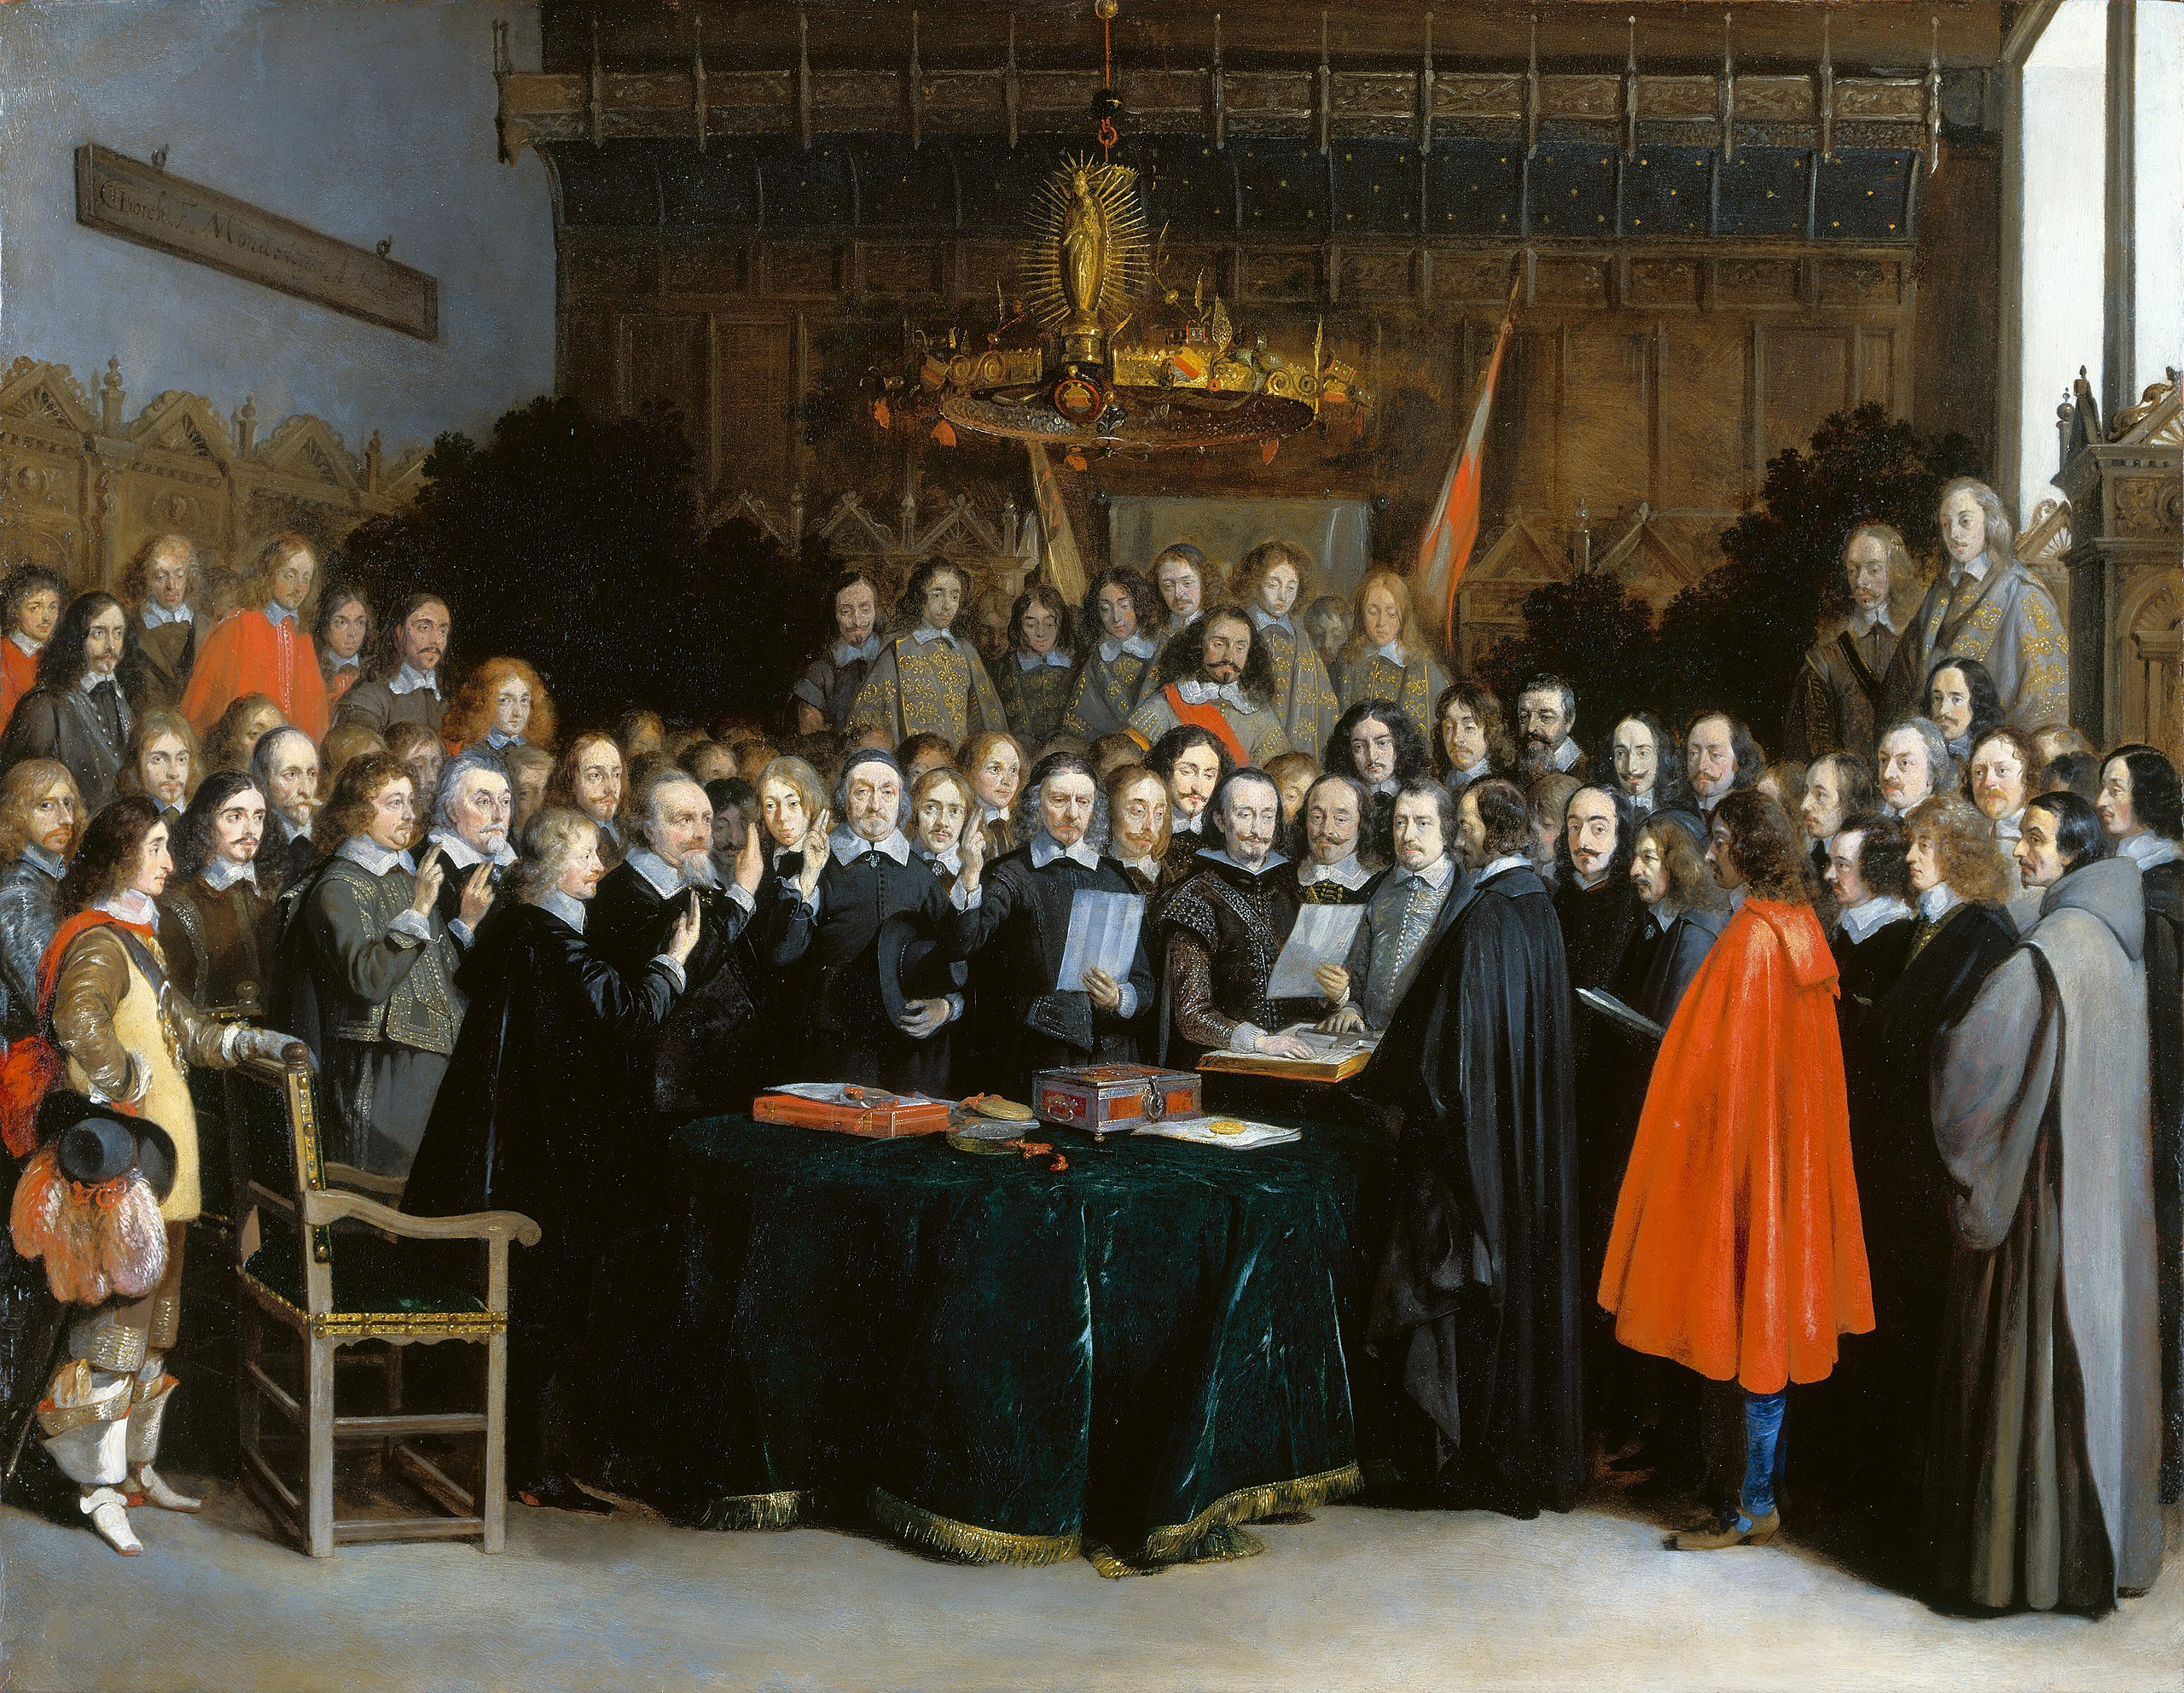
\includegraphics[keepaspectratio]{images/westfalia.jpg}}

}

\caption{Ratificación de uno de los tratados que se conocen como la Paz
de Westfalia por Gerard ter Borch}

\end{figure}%

Antes de Westfalia, Europa estaba organizada bajo un sistema feudal y
religioso en el que el poder político y judicial estaba fragmentado. La
Iglesia, los señores feudales y el Sacro Imperio Romano Germánico
compartían y competían por la autoridad sobre territorios y poblaciones.
La justicia no era uniforme; coexistían tribunales eclesiásticos,
jurisdicciones señoriales y cortes reales, cada una con diferentes
criterios de legitimidad y aplicación de la ley.

\begin{tcolorbox}[enhanced jigsaw, bottomtitle=1mm, toprule=.15mm, colbacktitle=quarto-callout-note-color!10!white, bottomrule=.15mm, leftrule=.75mm, colframe=quarto-callout-note-color-frame, opacitybacktitle=0.6, titlerule=0mm, breakable, colback=white, left=2mm, arc=.35mm, title=\textcolor{quarto-callout-note-color}{\faInfo}\hspace{0.5em}{Nota}, toptitle=1mm, coltitle=black, rightrule=.15mm, opacityback=0]

\textbf{¿Y por aquí}

En la Peninsula Ibérica no existía aún España. Teniamos la monarquía
hispánica: un conjunto de reinos, señoríos y territorios que compartían
un mismo monarca (el rey ``de las Españas''), pero cada uno mantenía sus
propias leyes, instituciones, monedas y sistemas fiscales. El rey
gobernaba cada uno de estos territorios según sus propios fueros y
consejos (Consejo de Castilla, de Aragón, de Italia, de Indias, etc.).
No existía una administración centralizada ni una identidad nacional
común. Los súbditos solían identificarse como castellanos, aragoneses,
napolitanos o flamencos, más que como ``españoles'' en sentido político.
No había un único sistema judicial unificado, sino múltiples
jurisdicciones que dependían de cada reino, ciudad o señorío. Era un
sistema complejo, desigual y fuertemente marcado por el carácter
estamental y religioso del Antiguo Régimen. La pena debía servir para
atemorizar y escarmentar más que para rehabilitar y las autoridades
tenían un gran margen para interpretar la ley y fijar penas.

\end{tcolorbox}

Con la Paz de Westfalia, se estableció el principio de soberanía
estatal, que otorgaba a cada Estado la autoridad exclusiva sobre su
territorio y población, incluyendo la administración de la justicia.
Este cambio significó una centralización del poder y una mayor
uniformidad en la aplicación de la ley.

Uno de los logros más importantes de los tratados de Westfalia fue el
reconocimiento formal de la soberanía estatal. Este principio establecía
que cada Estado tenía autoridad exclusiva sobre su territorio y asuntos
internos, sin interferencia externa. De ahí, que se reconozca este
tratado como fundamental en la génesis de los Estados modernos.

La aparición del Estado moderno tuvo su repercusión en el control del
delito. En el ámbito de la justicia penal, esto significó que el Estado
asumió el monopolio de la aplicación de la ley y el castigo de los
delitos, reemplazando a las autoridades eclesiásticas y feudales que
anteriormente compartían esta función.

La centralización del poder permitió la creación de sistemas judiciales
más coherentes y uniformes, basados en códigos legales nacionales y
procedimientos estandarizados. Esto sentó las bases para el desarrollo
del Estado de derecho y la consolidación de sistemas de justicia penal
modernos.

Antes de Westfalia, la justicia penal estaba estrechamente vinculada a
la moral religiosa. Los tribunales eclesiásticos juzgaban conductas
consideradas pecaminosas, como la herejía o la blasfemia, que a menudo
coincidían con delitos penales. Con la Paz de Westfalia y la
consagración del principio de soberanía estatal, se inición un largo
proceso de secularización del derecho. La administración de la justicia
pasó a estar bajo el control exclusivo del Estado, y las leyes tendieron
a basarse en principios laicos, en lugar de en doctrinas religiosas.

Este cambio permitió una mayor ``objetividad'' y ``coherencia'' en la
aplicación de la ley, y facilitó la evolución de sistemas de justicia
penal que se centraban en la protección del orden social y la seguridad
pública, en lugar de en la salvación del alma (aunque el proceso de
secularización se prolongó de forma notable durante los siglos
venideros).

La Paz de Westfalia marcó el nacimiento del Estado moderno, y con él, el
surgimiento de un nuevo modo de entender la justicia y el castigo. Al
consolidar la soberanía, la territorialidad y la secularización del
poder, estableció las condiciones necesarias para que los Estados
asumieran el monopolio legítimo de la violencia, crearan sistemas
legales unificados y desarrollaran instituciones judiciales racionales.
La centralización del poder y la autoridad exclusiva del Estado sobre la
ley crearon las condiciones necesarias para que, en el siglo XVIII,
pensadores de la Ilustración como Cesare Beccaria y Jeremy Bentham
pudieran conceptualizar un sistema penal racional, humano y codificado.

\section{La llamada Escuela Clásica y la reforma del derecho
penal}\label{la-llamada-escuela-cluxe1sica-y-la-reforma-del-derecho-penal}

En los siglos XVII y XVIII, los sistemas de justicia penal en Europa
eran fragmentados, arbitrarios y frecuentemente crueles. La autoridad
judicial se dividía entre tribunales eclesiásticos, jurisdicciones
señoriales y cortes reales, lo que generaba inconsistencias en la
aplicación de la ley. Los castigos eran desproporcionados y brutales: la
tortura se utilizaba con frecuencia para obtener confesiones, y las
ejecuciones públicas eran espectáculos destinados a infundir temor en la
población. Además, la justicia estaba profundamente ligada a la moral y
la religión; muchos delitos eran percibidos como pecados, y el castigo
cumplía tanto una función retributiva como espiritual.

\begin{figure}[H]

{\centering \pandocbounded{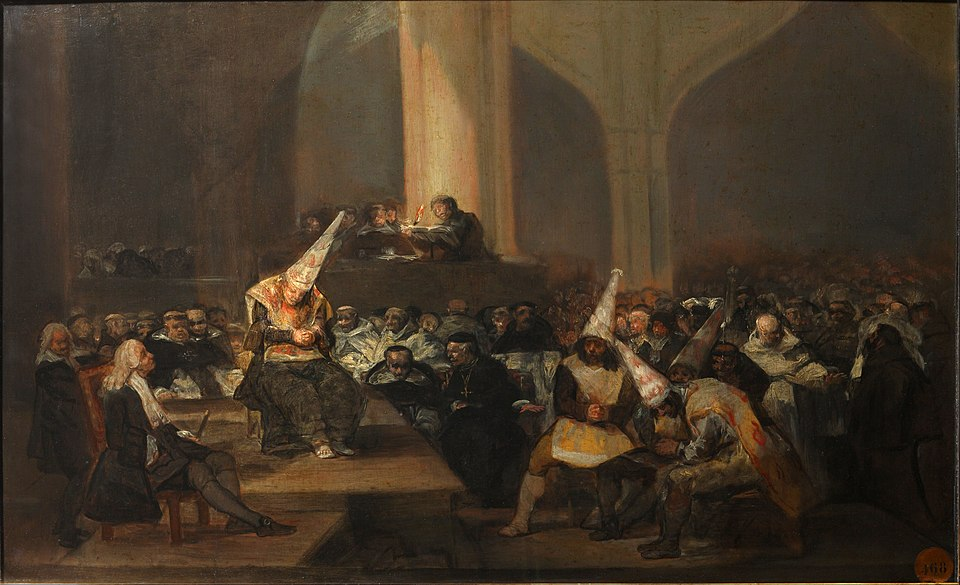
\includegraphics[keepaspectratio]{images/goya_1.jpg}}

}

\caption{Auto de fe de la inquisición pintado por Francisco Goya}

\end{figure}%

Este contexto mostraba la necesidad de un cambio profundo. La
consolidación de Estados soberanos tras Westfalia ofrecía un marco legal
uniforme, pero la práctica aún carecía de principios racionales,
consistencia y protección de los derechos de los acusados. Era este
escenario el que Beccaria y otros pensadores ilustrados criticaron,
proponiendo alternativas basadas en la razón, la utilidad social y la
proporcionalidad.

Estos autores están vinculados al periodo conocido como la Ilustración
que eventualmente vendrían ligados a cambios políticos, sociales y
económicos importantes (p.ej., la Revolución Francesa de 1789). La
Ilustración fue un movimiento humanista filosófico que pensaba que la
razón y el conocimiento empírico tenía que sustituir a la fe y la
superstición como bases de una sociedad moderna. Los autores asociados a
este movimiento intelectural proponían que la base de la comunidad
política se debía construir sobre un contrato social entre ciudadanos,
clases pudientes y poder político. Los ciudadanos tenían que ceder parte
de sus libertades para que el poder político pudiera desarrollar y
aplicar las leyes en beneficio del bien común. La autoridad legal
debería emanar de este contrato social y no de la teología. Quienes
vulnerasen las leyes impuestas por esta autoridad legal, a través del
proceso del contrato social, deberían ser castigados para preservar el
bien común, pero siempre y cuando este castigo se impusiera de forma
razonable. Surge también la idea durante este periodo de la separación
de poderes (ejecutivo, legislativo y judicial) que sigue estructurando
nuestro ordenamiento constitucional.

\subsection{Cesare Beccaria}\label{cesare-beccaria}

Cesare Beccaria (1738--1794), filósofo y jurista italiano, es
considerado uno de los fundadores del derecho penal moderno. Su obra
\emph{Dei delitti e delle pene} (1764) marcó un antes y un después en la
conceptualización del castigo y la justicia penal. Beccaria fue
influenciado por pensadores como Montesquieu, cuyo análisis de la
separación de poderes y la proporcionalidad de las leyes inspiró su
visión, y por Rousseau, cuya noción de contrato social fundamentaba la
legitimidad de las leyes como expresión de la voluntad colectiva.
También se basó en la tradición jurídica romana, que promovía la
codificación y racionalización del derecho.

\begin{figure}[H]

{\centering \pandocbounded{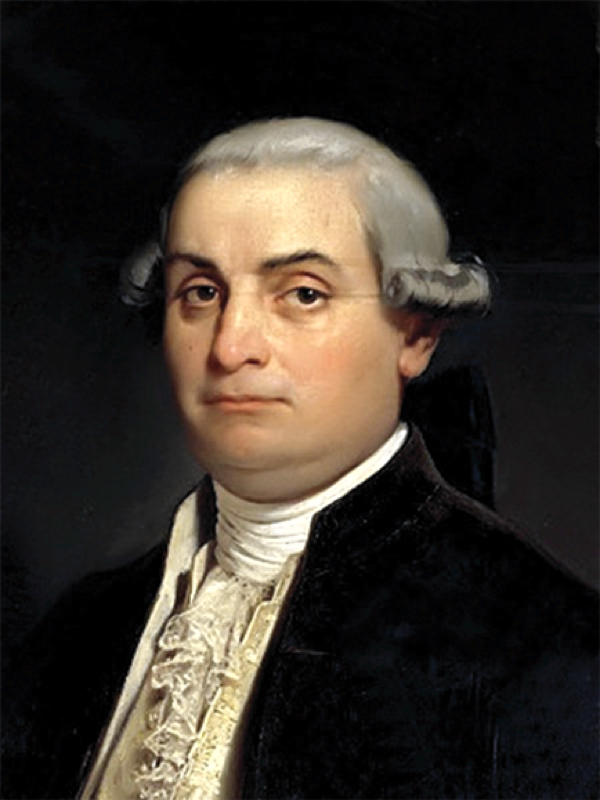
\includegraphics[keepaspectratio]{images/Cesare_Beccaria.jpg}}

}

\caption{Cesare Beccaria por Eliseo Sala}

\end{figure}%

Beccaria criticó abiertamente la arbitrariedad de los sistemas penales
de su tiempo, la tortura, los castigos excesivos y la pena de muerte.
Propuso que las leyes fueran claras, públicas y aplicadas de manera
uniforme, y que las penas fueran proporcionales a los delitos. Destacó
que la función principal del castigo debía ser prevenir futuros delitos,
en lugar de satisfacer un sentido de venganza o moralidad religiosa.
Además, defendió garantías procesales, a través de juicios rápidos y
públicos, limitando la discrecionalidad de jueces y autoridades.

Su tratado era, por tanto, un manifiesto en favor una concepción liberal
del Derecho Penal frente a los abusos de las monarquías absolutas. En
realidad sus ideas no eran particularmente originales, reflejaban el
sentir de muchos intelectuales del período, y él tomaba prestadas ideas
de muchos autores (a los que por temor a la Inquisición no citaba). La
primera versión de su tratado, de hecho, fue escrita por uno de sus
amigos (Pietro Verri) sobre la base de conversaciones con Beccaria.

En 1765 tras el éxito en Italia fue traducido y reivindicado en francés
por autores como Voltaire (que en ediciones posteriores a 1766 añadió
sus comentarios). En 1800 se habían publicado ya 23 ediciones italianas,
14 francesas, y 11 en inglés, dando así muestra de su popularidad y
buena acogida. En parte su fama se debió que la Iglesia católica
prohibió el libro como contrario a la fe por su excesivo racionalismo y
lo incluyó en el \emph{Index Prohibitorium} en 1766.

Muchos autores citan a Beccaria como el padre de una ``escuela clásica
de criminología'' y destacan que al hablar, en su trabajo, del calculo
penal del delincuente esta subrayando su capacidad para actuar
libremente (tan solo guiado por el coste de costes y beneficios
penales). No obstante, esta es una visión muy superficial de sus
escritos y probablemente una malinterpretación de sus influencias
intelectuales. Beccaria en su texto insiste en que el delincuente y la
delincuencia tienen que ser entendidos causalmente en términos de sus
circunstancias sociales y materiales (no en términos puramente de
calculo racional individualista). Beccaria posiblemente mantenía una
concepción de la ``agencia humana'' que incluía elementos de calculo
racional ``libre'' y de acción ``determinada'' por las circunstancias
sociales (Beirne 1993).

Por tanto, la importancia histórica de Beccaria no reside en haber
generado una teoría criminológica sobre el hombre delincuente, sino que
radica en que tradujo las condiciones políticas creadas por Westfalia
---la soberanía estatal y el monopolio del castigo--- en principios
jurídicos racionales, creando un marco conceptual para sistemas penales
codificados y humanos.

\begin{tcolorbox}[enhanced jigsaw, bottomtitle=1mm, toprule=.15mm, colbacktitle=quarto-callout-note-color!10!white, bottomrule=.15mm, leftrule=.75mm, colframe=quarto-callout-note-color-frame, opacitybacktitle=0.6, titlerule=0mm, breakable, colback=white, left=2mm, arc=.35mm, title=\textcolor{quarto-callout-note-color}{\faInfo}\hspace{0.5em}{Nota}, toptitle=1mm, coltitle=black, rightrule=.15mm, opacityback=0]

\textbf{¿Podemos hablar de una Escuela Clásica de criminología}

Aunque a menudo se citan a Beccaria y a Bentham como los flamantes
integrantes de dicha escuela, otros autores sostienen que ni era una
escuela, ni era criminología. Con esta etiqueta se fuerza la asimilación
de autores a un proyecto científico (la criminología) que no fue
realmente inventada hasta décadas más tarde. Sí es verdad que estos
autores compartían una visión del delincuente como un ser humano normal
que en su delinquir no hacía más que satisfacer necesidades y
aspiraciones humanas básicas. Pero, aunque muchos manuales proponen un
debate entre determinismo y agencia humana (libre albedrio)
contraponiendo el positivismo criminológico que surgiría después y los
proponentes de la escuela clásica, este es un debate un tanto ficticio
en cuanto que los autores clásicos no ignoraban fuerzas deterministas.
El interés de estos autores estaba más centrado en la reforma de la
justicia penal que en el entendimiento de la delincuencia. Algunas ideas
estaban influidas por una agenda humanista y progresista y fueron muy
influyentes al guiar pensamiento y práctica posterior: prevención a
través de la disuasión, la necesidad de una buena ley y administración
de justicia, etc. Pero también tenían ideas que eran conservadoras
incluso para aquella época.

\end{tcolorbox}

Desde un punto de vista histórico, la influencia de Beccaria fue
determinante en la modernización de códigos penales en Europa y sentó
las bases para sistemas de justicia penal basados en principios
universales de legalidad y derechos procesales del acusado.

\subsection{Jeremy Bentham}\label{jeremy-bentham}

Jeremy Bentham (1748--1832), filósofo y jurista británico, complementó y
sistematizó las ideas de Beccaria desde la perspectiva del utilitarismo.
Inspirado por Beccaria y por filósofos como John Locke y David Hume,
Bentham propuso que las leyes y los castigos debían organizarse de
manera que maximizaran el bienestar general y minimizaran el daño.
Introdujo la noción de un ``cálculo hedonista'' para evaluar la
intensidad, duración, certeza y prontitud de la pena, con el objetivo de
lograr la máxima disuasión posible.

Bentham se graduó por la Universidad de Oxford a tierna edad de los doce
años. Fue un autor que escribió ampliamente sobre filosofía moral,
derecho, penología, jurisprudencia y policía. Estuvo influenciado por
Beccaria y el filosofo escoces David Hume. Como Beccaria quería un
régimen legal racional, humano y codificado en un cuerpo transparente de
leyes, pero en lugar de compilar una serie de propuestas humanistas
contra las practicas barbáricas del sistema penal como hizo Beccaria, se
propuso ofrecer una base filosófica solida a lo que debería ser la nueva
penología.

Hume argumentaba que la base de la acción moral es la producción de la
felicidad. Bentham adotó esta idea y propuso un sistema filosófico que
aspiraba a que el derecho estuviera orientado a conseguir la mayor
felicidad del mayor número de personas (una concepción utilitarista e
instrumental del derecho).

Bentham partía de una explicación hedonista del comportamiento humano
que actúan como actores racionales:

\begin{quote}
``La naturaleza ha sometido a la humanidad al dominio de dos soberanos
amos: el dolor y el placer. Solo ellos pueden indicarnos lo que debemos
hacer, así como determinar lo que haremos''
\end{quote}

Para Bentham nuestro comportamiento se guía, así, por la búsqueda del
placer y la evitación del dolor (ambas son ``percepciones
interesadas''). Según Bentham, siguiendo este modelo, si cometemos
delitos es porque nos sirve para obtener ``placer'' o evitar ``dolor''.

De ello, si el delincuente persigue la obtención de ``placer'' y
evitación de ``dolor'', Bentha derivaba que el legislador penal debe
tener en cuenta este calculo a la hora de diseñar las sanciones penales.
El delito se puede prevenir por medio de sanciones positivas
(recompensas) o sanciones negativas (castigos). Para Bentham, el
legislador debería seguir cuatro reglas penológicas para calcular la
proporción entre delitos y penas:

\begin{itemize}
\item
  El fin de la ley penal es la prevención por tanto el legislador
  debería asegurarse que el ``placer'' obtenido por la realización del
  delito fuera contrarrestado por el ``dolor'' de la sanción penal.
\item
  La amenaza de esta sanción, por sí sola, debería ser suficiente para
  que el delincuente se abstuviera o en todo caso cometiera un delito
  menor.
\item
  El castigo no debería ser excesivo si queremos que el delincuente, al
  delinquir, no vaya más allá de lo que le es estrictamente necesario.
\item
  Los legisladores deberían tratar de que el castigo penal fuera lo más
  económico posible.
\end{itemize}

Bentham también introdujo el concepto de ``panóptico'' como modelo de
diseño de prisiones orientadas al control eficiente y sostenía que la
certeza, prontitud y proporcionalidad del castigo eran más importantes
que su severidad extrema. Su enfoque utilitario ofreció una metodología
práctica para que los Estados aplicaran la justicia penal de manera
eficiente, transparente y orientada al beneficio social.

Bentham, al igual que Beccaria, aprovechó las condiciones creadas por la
soberanía estatal post-Westfalia: el monopolio del castigo por parte del
Estado permitió que la administración de justicia se diseñara según
principios racionales, en lugar de depender de arbitrariedades locales o
de la Iglesia. Su trabajo ayudó a consolidar un sistema de justicia
penal preventivo y organizado, que se convirtió en un modelo para la
modernización legal en Inglaterra y en otros países europeos.

\begin{figure}[H]

{\centering \pandocbounded{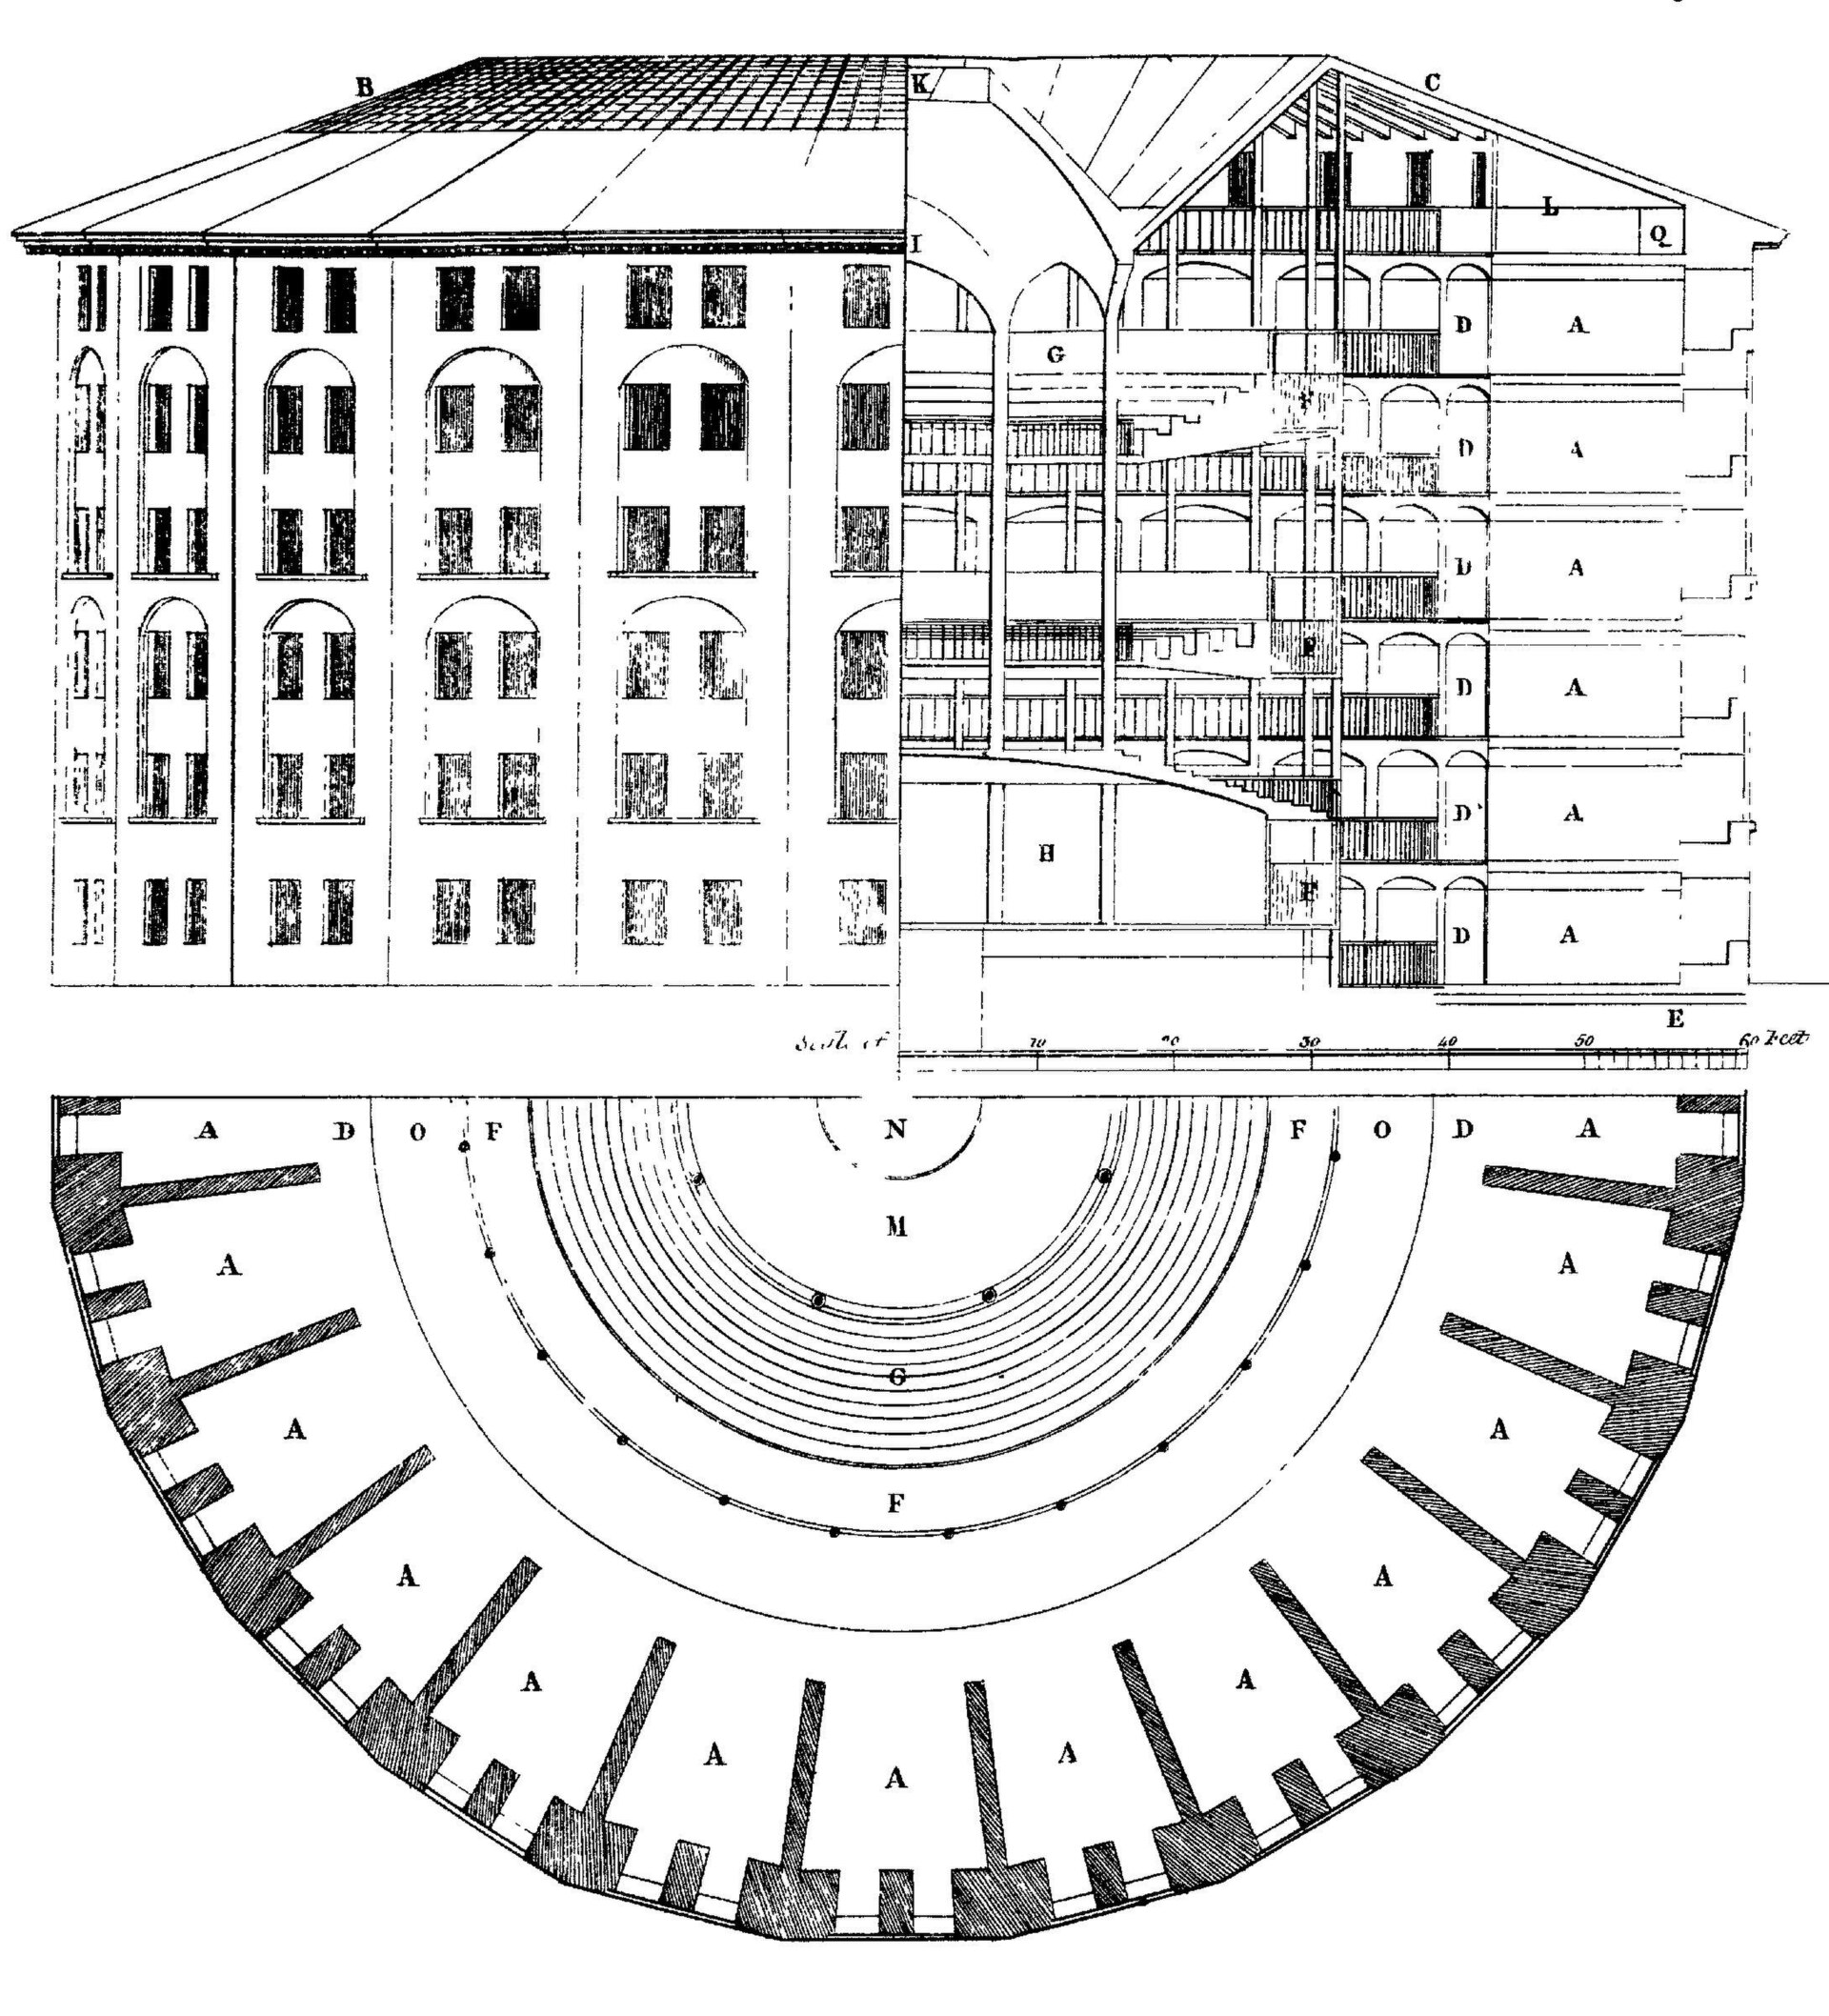
\includegraphics[keepaspectratio]{images/Panopticon.jpg}}

}

\caption{Diseño del panóptico de Jeremy Bentham}

\end{figure}%

Desde un punto de vista histórico, se puede trazar una línea clara: la
Paz de Westfalia estableció el marco político, garantizando soberanía,
centralización y secularización; Beccaria proporcionó los principios
morales y racionales para un sistema penal humano y predecible; y
Bentham ofreció la metodología utilitaria y sistemática para aplicar la
justicia de manera eficiente y socialmente beneficiosa. Juntos, estos
elementos transformaron la justicia penal: de un sistema fragmentado,
arbitrario y frecuentemente cruel, a uno codificado, racional,
preventivo y administrado por el Estado moderno.

\section{La invención de la policía y la
prisión}\label{la-invenciuxf3n-de-la-policuxeda-y-la-prisiuxf3n}

Vemos así, como desde el siglo XVII al XVIII se fueron fraguando las
bases políticas y filosóficas que servirían para armar el actual sistema
de justicia penal. Elementos claves en este proceso fueron la invención
de la prisión como castigo y de la policía como institución de custodia
del derecho y mantenimiento de la paz social. Aunque a muchas personas
les pueda parecer impensable el vivir en sociedades sin prisiones o
policias, la humanidad ha vivido sin ellos durante la mayor parte de su
existencia. Ambas instituciones son invenciones modernas que se van
desarrollando durante el siglo XIX hasta adquirir la forma que tienen
hoy en día.

El surgimiento de la prisión y la policía como instituciones centrales
del Estado moderno constituyen uno de los procesos más significativos de
la historia contemporánea. Ambas surgieron entre los siglos XVIII y XIX,
en el contexto de la consolidación del Estado soberano y de las
transformaciones sociales que trajo consigo la modernidad capitalista.
Su aparición no solo respondió a una necesidad técnica de organización
del orden público o de reforma del castigo, sino que también reflejó
---y consolidó--- una nueva relación de poder entre las clases sociales,
en la que el control, la vigilancia y la disciplina se convirtieron en
herramientas fundamentales de dominación política y económica.

Como ya hemos recalcado, antes del surgimiento del Estado moderno, la
justicia en Europa estaba marcada por la fragmentación jurisdiccional.
Los señores feudales, la Iglesia y los tribunales reales compartían la
autoridad sobre el castigo. Las penas eran públicas, crueles y
ejemplares: horcas, torturas, mutilaciones o destierros buscaban
infundir miedo más que corregir. No existían la prisión ni la policía
como hoy las entendemos. La reclusión se usaba solo de manera temporal,
y el control del orden dependía de milicias locales o de comunidades
vecinales.

Tras la Paz de Westfalia (1648), el Estado soberano asumió el monopolio
del uso legítimo de la fuerza y comenzó a centralizar la administración
de justicia. Este proceso, sin embargo, no implicó inmediatamente una
humanización del castigo, sino su racionalización política: el poder
punitivo pasó a ser un atributo exclusivo del Estado. En este contexto
surgieron, durante los siglos XVIII y XIX, la policía y la prisión como
instrumentos modernos de control social.

El concepto de policía evolucionó junto con la idea de Estado. En el
siglo XVII, \emph{police} en Francia designaba el ``buen gobierno'' o la
administración del orden público. La policía no era una institucion o
una organización sino un término que se usaba para identificar las
labores políticas locales. Policía originalmente significaba gobierno
municipal y, por tanto, sus funciones eran muy amplias.

\begin{figure}[H]

{\centering \pandocbounded{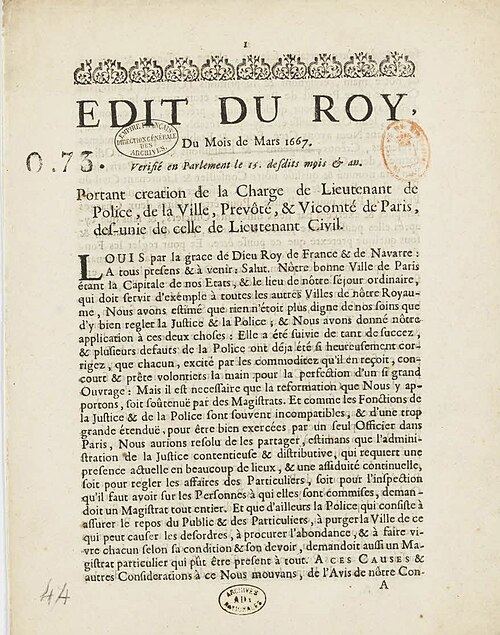
\includegraphics[keepaspectratio]{images/edicto.jpg}}

}

\caption{Edicto de creación del Teniente general de policía}

\end{figure}%

Fue bajo Luis XIV, en 1667, cuando se creó en París el cargo de
\emph{lieutenant général de police}, el Teniente general de policía,
considerado el origen de la policía moderna. Este cargo posteriormente
se convertiría en un Ministerio durante la Revolución y el período
Napoleónico. Era un cargo con poder normativo que permitía crear normas
con sanciones tan severas que a estos efectos se podrían considerar
normas penales. Era un cargo también con poder judicial en todas
aquellas materias que se consideraban no tenían que llegar a los
tribunales. La policía era el cargo y sus poderes, no el cuerpo de
agentes. Este edicto no creó un cuerpo de personas encargados de
garantizar el cumplimiento de la ley, aunque eventualmente el sistema de
policía de París evolucionó para contar con una fuerza armada de hombres
(algunos con formación militar). Los hombres al servicio del Teniente
contaban con 3 inspectores que practicaban detenciones informados por
una amplia red de informantes policiales y ``soplones''. Este cargo
tenía la función de vigilar, controlar y disciplinar a la población
urbana, un espacio en el que el crecimiento demográfico, la pobreza y el
comercio empezaban a generar tensiones sociales. El control de la
opinión pública era igualmente importante, así como la represión de la
disidencia religiosa o política. El control de la opinión se contemplaba
como una forma de ``mantener el orden'' dada la creencia de que las
``ideas peligrosas'' eran la fuente de problemas. ¿Quién era el
``objeto'' de la acción policial en Paris? Fundamentalmente los pobres
sin trabajo. Este proletariado era el objetivo obvio por varias razones:
se le consideraba responsable de los delitos y podían ser movilizados
para generar disturbios. La idea es que había que proteger a la clase
trabajadora de ser contaminada por este proletariado.

Durante el siglo XVIII, las ciudades europeas comenzaron a desarrollar
cuerpos similares. En Berlín, Viena o Madrid se establecieron
instituciones encargadas de vigilar las calles, censar a la población,
controlar el trabajo y la mendicidad, y reprimir la disidencia.

En Inglaterra, sin embargo, el desarrollo fue más tardío. No fue hasta
1829 que Sir Robert Peel fundó la \emph{Metropolitan Police} de Londres,
considerada la primera policía profesional y civil. Su objetivo
principal no era la represión abierta, sino la prevención del delito
mediante la vigilancia constante y la presencia pública.

\begin{figure}[H]

{\centering \pandocbounded{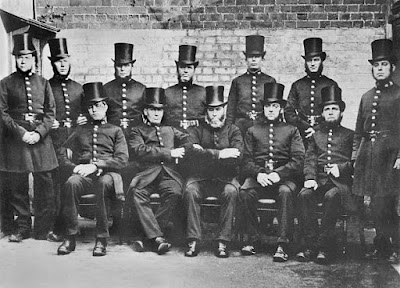
\includegraphics[keepaspectratio]{images/peelers.jpg}}

}

\caption{Imagén de los ``Peelers'', los hombres de Peel, que conformaron
la policía metropolitana de Londres}

\end{figure}%

Sir Robert Peel fue un reformista que quería mejorar la prevención del
delito. Tuvo que lidiar con quienes veían en la policía centralizada una
amenaza contra la libertad (lo que contribuyó al carácter menos militar
de la institución en el Reino Unido). Su creación en 1829 representó un
momento de ruptura que cambió el significado del termino policía:

\begin{itemize}
\item
  Hasta entonces había significado la gobernanza de un territorio en
  todos sus aspectos
\item
  La policía hasta entonces era un sistema autocontenido que poseía
  todos los atributos para ejercitar la gobernanza (legislativo,
  regulatorio, judicial, y ejecutivo)
\end{itemize}

En Londres se redujo el significado en dos sentidos:

\begin{itemize}
\item
  No era ya un sistema autocontenido, sino una rama del sistema de
  justicia penal, que se encargaba de poner a los delincuentes en manos
  del poder judicial
\item
  ``La policía'' empezó a ser el término que se empleaba para designar
  al conjunto de hombres encargados de hacer labores policiales, que
  empezaron a estar estrictamente limitadas a la provisión de la
  seguridad.
\end{itemize}

Aunque se presentaba como una institución al servicio de la seguridad
general, la policía moderna surgió en un contexto de creciente
conflictividad social. La expansión del capitalismo industrial y la
urbanización produjeron nuevas formas de pobreza y marginación. Las
clases dirigentes comenzaron a ver en la clase trabajadora un peligro
potencial para el orden. Así, la policía se convirtió en un instrumento
no solo de protección, sino de control de los sectores populares. Su
tarea era tanto mantener la ``paz'' como asegurar las condiciones
necesarias para la estabilidad del sistema económico.

\begin{figure}[H]

{\centering \pandocbounded{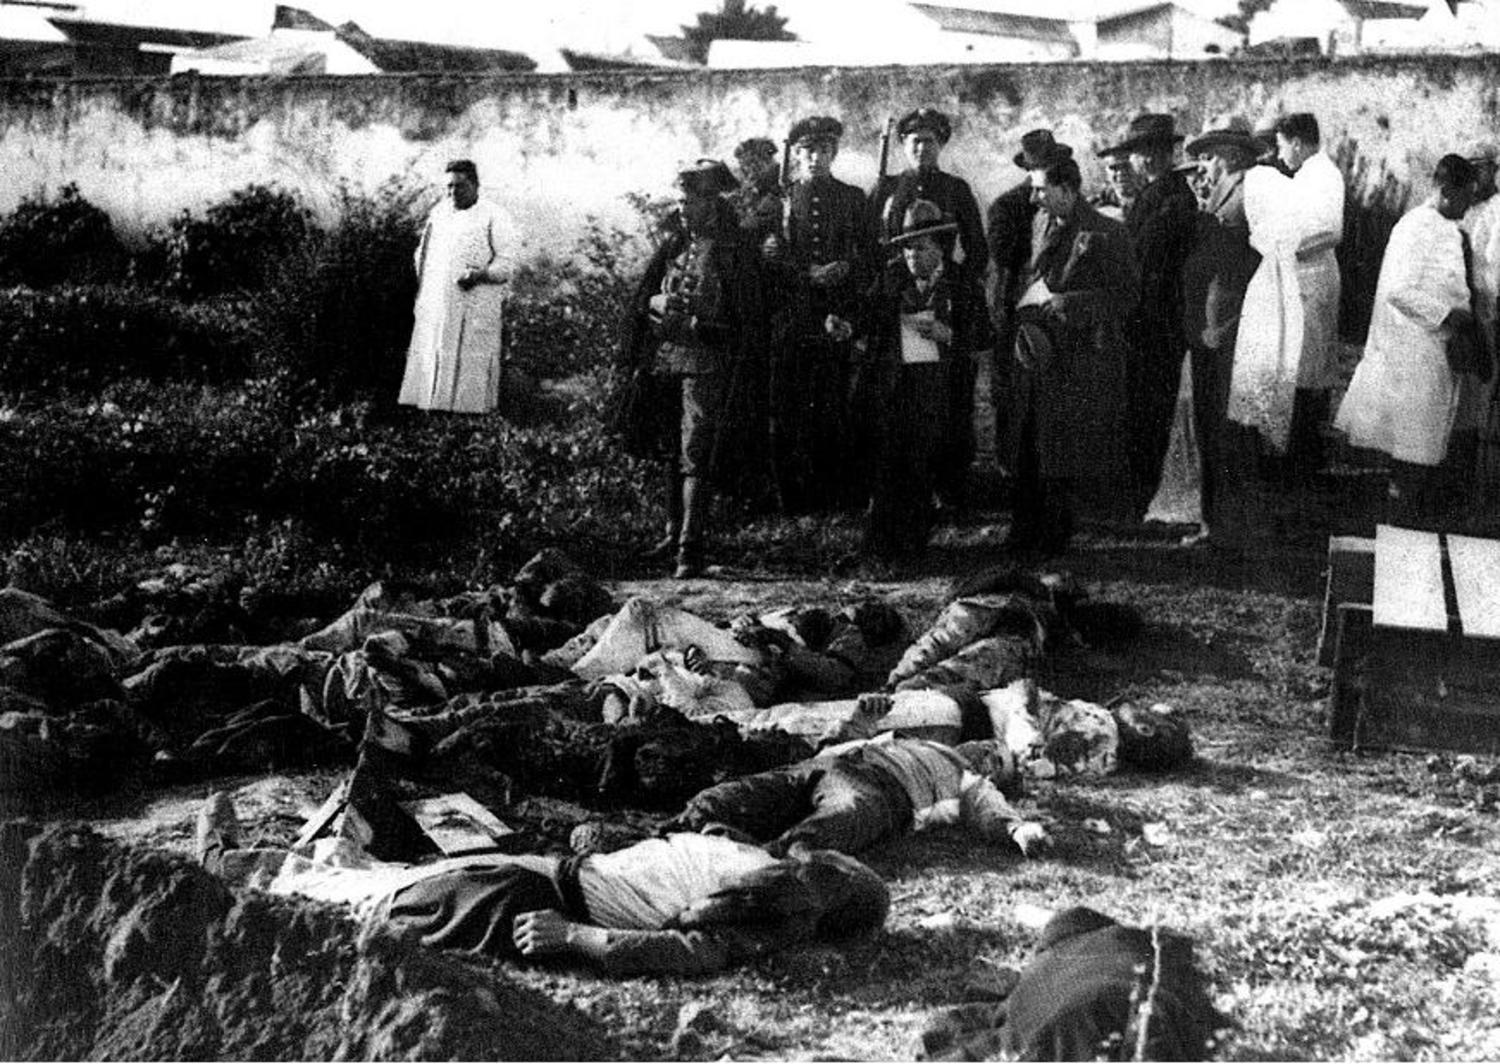
\includegraphics[keepaspectratio]{images/casasviejas.jpg}}

}

\caption{La Guardia Civil en Casas Viejas, símbolo de la represión del
campo andaluz.}

\end{figure}%

En paralelo al desarrollo de la policía, la prisión moderna emergió como
resultado de las reformas ilustradas del derecho penal. Como ya hemos
visto, hasta el siglo XVIII, el castigo se entendía como un espectáculo
público, donde la violencia del soberano se ejercía directamente sobre
el cuerpo del condenado. Sin embargo, pensadores como Cesare Beccaria y
Jeremy Bentham plantearon que la pena debía ser útil, racional y
proporcional. Beccaria rechazó la tortura y la pena de muerte,
proponiendo la privación de libertad como una alternativa más humana y
eficaz. Bentham, por su parte, diseñó el modelo del Panóptico, una
arquitectura carcelaria que permitía la vigilancia total de los presos,
simbolizando la transición del poder punitivo al poder disciplinario.

La prisión se convirtió así en el espacio donde el castigo se
transformaba en disciplina. Michel (\textbf{Foucault\_75?}), en su muy
influyente \emph{Vigilar y castigar}, describió este cambio como el paso
del ``suplicio del cuerpo'' a la ``corrección del alma''. El objetivo ya
no era destruir al delincuente, sino reformarlo, moldearlo para
adaptarlo a las normas de la sociedad industrial. Este nuevo régimen
punitivo coincidió con el ascenso del capitalismo: la prisión servía
para encerrar y controlar a quienes no se integraban en la lógica del
trabajo asalariado ---vagabundos, desempleados, pobres, disidentes---,
convirtiéndose en una herramienta de regulación del trabajo y de la
moral social. Para Melossi y Pavarini (1980) la cárcel moderna surge
como parte integrante del dispositivo disciplinario del capitalismo,
destinado a producir sujetos obedientes, disciplinados, útiles para la
fábrica (o la economía capitalista), mediante prácticas de segregación,
castigo, trabajo, y disciplina.

Tanto la policía como la prisión surgieron como instrumentos de control
social al servicio del nuevo orden económico y político. La policía
actuaba en el espacio público, garantizando la seguridad de la propiedad
privada y la disciplina laboral; la prisión actuaba en el espacio
cerrado, reformando a los individuos que transgredían las normas del
trabajo y la moral.

En las ciudades industriales del siglo XIX, las huelgas, los motines y
las revueltas obreras fueron reprimidos con violencia policial. La
vigilancia de los barrios populares, la regulación del ocio y la
persecución del vagabundeo se convirtieron en prácticas cotidianas. Del
mismo modo, las cárceles comenzaron a llenarse de personas de baja
extracción social. El delito se asociaba a la miseria, y la miseria se
trataba como una amenaza al orden social.

La aparición de la prisión y la policía como instituciones estatales no
puede entenderse únicamente como un avance técnico o administrativo en
la gestión del orden. Ambas son el resultado de transformaciones
estructurales vinculadas al surgimiento del Estado moderno y al
desarrollo del capitalismo. En este nuevo orden, el castigo se volvió
racional, continuo y burocrático, pero también clase-específico: sirvió
para disciplinar a los sectores subalternos y garantizar la reproducción
del sistema social.

Así, la prisión y la policía deben ser comprendidas como pilares de la
modernidad política y económica, pero también como mecanismos de poder.
Su legitimidad se construyó sobre el discurso de la seguridad y la
justicia, pero su función práctica ha estado estrechamente ligada al
mantenimiento del orden social existente. En última instancia,
representan la institucionalización de la vigilancia y la coerción, los
dos rostros del control estatal moderno que, desde el siglo XIX hasta
hoy, continúan definiendo la relación entre Estado, ley y clase social.
Este tipo de interpretaciones, aunque avanzadas por algunos autores de
orientación marxista como Rusche y Kirchheimer (1939), no comenzó a ser
más aceptada hasta muy bien entrado el siglo XX, ya en la década de los
años 1960 y 1970.

\section{Correccionalismo y
rehabilitación}\label{correccionalismo-y-rehabilitaciuxf3n}

Ya hemos avanzado como a lo largo del siglo XIX y la primera mitad del
XX, el encierro se transformó de castigo físico y retributivo en un
instrumento de corrección moral, educación y tratamiento del
delincuente. En este proceso confluyeron tres corrientes fundamentales:
el correccionalismo jurídico, la influencia religiosa y filantrópica y,
más tarde, la psicología y la criminología positivista.

El siglo XIX supuso una verdadera revolución en las ideas sobre el
castigo. Frente al modelo retributivo heredado del Antiguo Régimen
---caracterizado por la violencia pública y la ejemplaridad---, emergió
un nuevo ideal: la corrección del delincuente. Este cambio fue influido
por los filósofos ilustrados como Beccaria y Bentham, pero se consolidó
en la práctica penitenciaria con la aparición de los sistemas de
Filadelfia y Auburn, basados en el aislamiento, el trabajo y la
introspección moral y con un sustrato religioso.

La religión, especialmente el cristianismo, desempeñó un papel central
en el desarrollo del sistema penitenciario moderno. Desde sus orígenes,
la prisión estuvo asociada al arrepentimiento y la conversión moral,
nociones profundamente enraizadas en la tradición cristiana.

En las primeras cárceles del siglo XIX, las órdenes religiosas y
asociaciones filantrópicas tuvieron un papel protagónico. Capellanes y
misioneros visitaban regularmente las prisiones para promover la lectura
de la Biblia, la oración y la reflexión. En Inglaterra y Estados Unidos,
los cuáqueros fueron particularmente influyentes en el diseño del
sistema penitenciario pensilvano, concibiendo la prisión como un lugar
de retiro espiritual donde el individuo, aislado del mundo, pudiera
reconciliarse con Dios.

La moral religiosa se entrelazó con el pensamiento correccionalista en
la construcción de la idea de culpa y redención. El delito se
interpretaba como una falta moral, pero también como una oportunidad de
salvación. Esta concepción legitimó prácticas penitenciarias basadas en
el aislamiento, la introspección y el trabajo silencioso, entendidos
como medios para purificar el alma del reo.

Sin embargo, esta dimensión religiosa también tuvo un componente
disciplinario. El discurso de la redención sirvió para moralizar y
domesticar a las clases trabajadoras y marginales, imponiendo valores
como la obediencia, la sobriedad y la sumisión. En este sentido, la
religión no solo ofreció consuelo, sino que también funcionó como
instrumento de control social, contribuyendo a la internalización de la
autoridad y del orden.

El sistema pensilvano, implementado en Filadelfia a inicios del siglo
XIX, promovía el aislamiento total del preso, bajo la idea de que el
recogimiento y la reflexión moral lo conducirían al arrepentimiento. Por
su parte, el sistema auburniano, desarrollado en Nueva York, combinaba
el trabajo colectivo con el silencio absoluto, entendiendo el trabajo
como medio de disciplina y redención. Ambos modelos reflejaban una
mezcla de pensamiento correccionalista y moral religiosa, en los que el
castigo corporal era reemplazado por la vigilancia, el trabajo y la
introspección.

La prisión, así, dejó de concebirse como un simple espacio de
sufrimiento y se transformó en una institución presuntamente pedagógica.
El castigo debía servir para reformar al delincuente y reintegrarlo a la
sociedad. Este giro coincidió con el ascenso del Estado liberal y
burgués, que veía en el orden y la disciplina social condiciones
indispensables para el progreso económico.

España no fue ajena a esta transformación. Durante la segunda mitad del
siglo XIX, se multiplicaron las reflexiones sobre la ``cuestión
penitenciaria'', impulsadas tanto por juristas como por filántropos y
pensadores sociales. En ese contexto emergió una figura decisiva:
Concepción Arenal (1820--1893).

\begin{figure}[H]

{\centering \pandocbounded{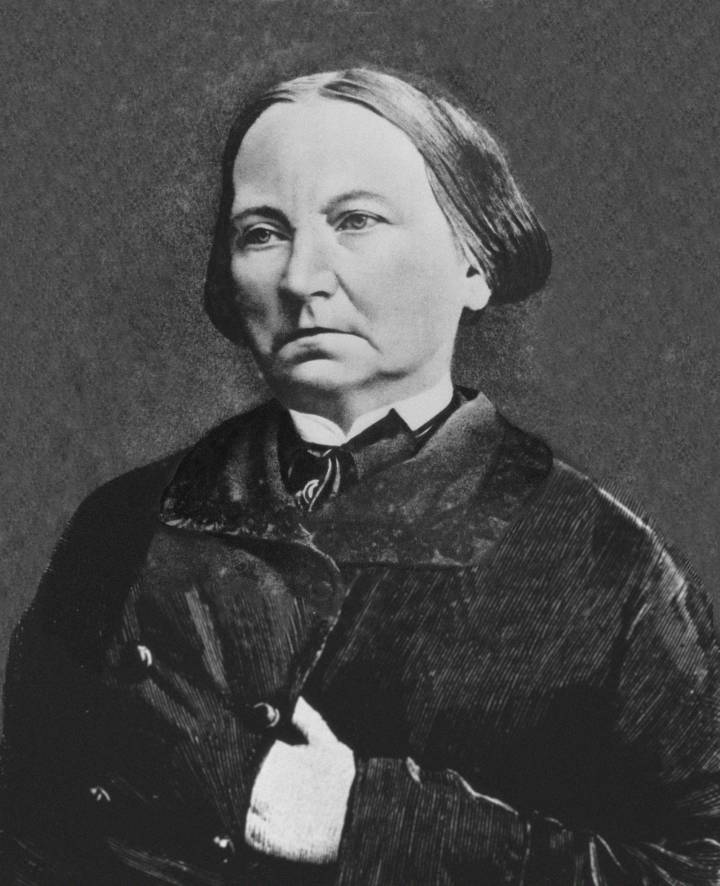
\includegraphics[keepaspectratio]{images/concepcion_arenal.jpg}}

}

\caption{Imagen de Concepción Arenal}

\end{figure}%

Concepción Arenal, jurista, escritora y reformadora social, fue una de
las voces más influyentes del pensamiento penal español del siglo XIX.
Su obra se situó en la encrucijada entre la filantropía cristiana, el
humanismo jurídico y el correccionalismo liberal. Arenal criticó
duramente la función puramente represiva de las cárceles y defendió un
modelo de reeducación moral y reinserción social del delincuente.

En textos como El visitador del preso (1863), La instrucción del pueblo
(1881) o Estudios penitenciarios (1895), Arenal planteó que el castigo
debía servir ``para corregir, no para vengar''. Su pensamiento se
apoyaba en una ética cristiana de la compasión y la dignidad humana: el
delincuente no era un enemigo del Estado, sino un ser humano que había
errado y debía ser ayudado a regenerarse.

Arenal fue también pionera en denunciar las condiciones infrahumanas de
las cárceles españolas y en promover la participación de las sociedades
de patronato y de protección al liberado. Consideraba que la cárcel
debía ser una institución educativa, en la que el trabajo, la
instrucción y la moral desempeñaran un papel redentor. En ese sentido,
anticipó ideas que más tarde se institucionalizarían en la criminología
moderna y en el discurso de la ``reinserción social''.

Su pensamiento, aunque fuertemente impregnado de valores religiosos,
trascendió el ámbito moral para cuestionar la raíz estructural de la
criminalidad. Arenal entendía el delito no solo como un fallo
individual, sino también como un producto de la pobreza, la ignorancia y
la injusticia social. Así, vinculó por primera vez en España la cuestión
penal con la cuestión social, abriendo el camino a una visión más
integral y crítica de la justicia.

A finales del siglo XIX, las ideas de Arenal coincidieron con la
expansión en Europa de la escuela correccionalista, que concebía la pena
como instrumento de prevención y readaptación. Juristas como Franz von
Liszt en Alemania o Enrico Ferri en Italia defendían un derecho penal de
fin práctico: no se castigaba por venganza moral, sino para proteger la
sociedad y corregir al delincuente mediante educación, trabajo y
disciplina.

Las ideas religiosas como legitimación de resocializacion penitenciaria
poco a poco fueron siendo desplazadas por otras ideas inspiradas en el
emergente pensamiento criminológico del siglo XIX. A fines del siglo XIX
y comienzos del XX, la psicología, la medicina y la criminología
positivista introdujeron un nuevo paradigma: el del delincuente como
anormal o enfermo. Inspirados en los avances científicos y en las
teorías evolucionistas, autores como Cesare Lombroso, Enrico Ferri y
Raffaele Garofalo propusieron que el crimen era producto de factores
biológicos, psicológicos y sociales, no simplemente de una decisión
moral.

Esta nueva mirada transformó la prisión en un laboratorio de observación
y tratamiento. Se introdujeron evaluaciones psiquiátricas,
clasificaciones de reclusos, programas de trabajo diferenciados y
medidas de ``tratamiento'' individualizado. El delincuente dejó de ser
visto como un pecador y pasó a ser considerado un paciente social que
debía ser diagnosticado, tratado y, si era posible, curado.

La influencia de la psicología se consolidó durante la primera mitad del
siglo XX, especialmente con el desarrollo del psicoanálisis y la
psicología conductista. En muchas prisiones europeas y latinoamericanas
se crearon servicios médicos, talleres de psicología y departamentos de
observación. El objetivo declarado era ``reeducar'' al delincuente,
aunque en la práctica esto reforzaba la dimensión disciplinaria y
normalizadora del sistema: la prisión no solo castigaba, sino que
también intentaba producir sujetos dóciles y adaptados.

La prisión moderna fue, al mismo tiempo, una institución moral,
científica y política. Desde la moral cristiana, buscaba el
arrepentimiento; desde el correccionalismo, la educación y el trabajo; y
desde la psicología, la adaptación del individuo a las normas sociales.
Sin embargo, todas estas perspectivas compartían una misma lógica: el
poder disciplinario, que transformaba el castigo físico en vigilancia
constante, introspección y auto-control.

En la primera mitad del siglo XX, especialmente tras la Segunda Guerra
Mundial, estas corrientes convergieron en la noción de tratamiento
penitenciario integral, que combinaba educación, asistencia psicológica,
y el trabajo. Este modelo, aún dominante en muchas legislaciones, hereda
las tensiones del siglo XIX: la promesa de rehabilitación convive con la
persistencia del control, la exclusión y la desigualdad.

\begin{tcolorbox}[enhanced jigsaw, bottomtitle=1mm, toprule=.15mm, colbacktitle=quarto-callout-note-color!10!white, bottomrule=.15mm, leftrule=.75mm, colframe=quarto-callout-note-color-frame, opacitybacktitle=0.6, titlerule=0mm, breakable, colback=white, left=2mm, arc=.35mm, title=\textcolor{quarto-callout-note-color}{\faInfo}\hspace{0.5em}{Nota}, toptitle=1mm, coltitle=black, rightrule=.15mm, opacityback=0]

\textbf{Resocialización en las carceles españolas durante el siglo XX}

Las nuevas teorías psicológicas de la resocialización tardaron en llegar
a nuestro país más que a otros. En España con la llegada del régimen
dictatorial franquista en 1939, el sistema penal y penitenciario adoptó
una orientación profundamente autoritaria e ideológica. La finalidad
principal de la pena no era la resocialización en sentido moderno (o de
la forma que se estaba interpretando en las democracias contemporaneas),
sino la ``reeducación moral'' del individuo conforme a los valores del
régimen: obediencia, religión, patria y disciplina. La prisión se
concebía como un espacio de control político y moral, donde el
delincuente, volviendo a las concepciones dominantes durante decadas
anteriores y superadas en otros países, debía ``purificarse'' mediante
el trabajo, la religión y la obediencia. Los presos políticos, en
particular, eran objeto de una reeducación forzada que buscaba su
sometimiento ideológico.

En este contexto, la resocialización se entendía más como
adoctrinamiento que como un proceso de reinserción libre y responsable.
Los programas penitenciarios se orientaban a la producción laboral
dentro de las cárceles, al cumplimiento estricto de la disciplina y a la
práctica religiosa obligatoria. Aunque se introdujeron algunas medidas
que podrían considerarse precursoras de la resocialización, como el
trabajo remunerado o la asistencia educativa, estas no respondían a una
concepción humanista del delincuente, sino a la necesidad de mantener el
orden y la productividad dentro de las prisiones. En definitiva, durante
el franquismo, la función resocializadora fue subordinada al control
ideológico y moral del individuo.

La transición democrática y la aprobación de la Constitución Española de
1978 marcaron un punto de inflexión decisivo. Por primera vez en la
historia española, la resocialización del delincuente se elevó a rango
constitucional. El artículo 25.2 de la Constitución establece que ``las
penas privativas de libertad y las medidas de seguridad estarán
orientadas hacia la reeducación y reinserción social''. Este precepto
supuso un cambio radical en la filosofía penal del Estado, al situar la
dignidad humana y la reintegración social en el centro de la política
penitenciaria. La pena dejó de concebirse exclusivamente como castigo y
pasó a entenderse como una oportunidad de transformación personal.

En desarrollo de este principio, se aprobó en 1979 la Ley Orgánica
General Penitenciaria (LOGP), que junto con su Reglamento de 1996,
estructuró un sistema penitenciario basado en la individualización del
tratamiento. El objetivo era ofrecer a cada interno un itinerario de
reinserción adaptado a sus circunstancias personales, sociales y
psicológicas. La LOGP introdujo medidas innovadoras, como los permisos
de salida, el régimen abierto, los trabajos en beneficio de la comunidad
y la atención educativa y laboral dentro de los centros penitenciarios.
Estas reformas reflejaron una visión más humanista del delincuente,
reconociéndolo como sujeto de derechos y no simplemente como objeto de
castigo.

En la actualidad, la resocialización sigue siendo el eje teórico y
normativo del sistema penitenciario español. Las prisiones cuentan con
programas de formación, trabajo, educación y atención psicológica
orientados a reducir la reincidencia. Se desarrollan programas
específicos para colectivos con problemáticas concretas, como
toxicómanos, agresores sexuales o personas condenadas por violencia de
género. Además, se fomenta la participación de organizaciones no
gubernamentales y entidades sociales en la labor de reinserción,
favoreciendo la colaboración entre la administración penitenciaria y la
sociedad civil.

Sin embargo, persisten importantes retos y contradicciones. A pesar del
marco legal avanzado, la efectividad real de la resocialización se ve
limitada por factores estructurales: la falta de recursos, la
sobrepoblación penitenciaria, el déficit de personal especializado y,
sobre todo, la dificultad de reintegración social tras la excarcelación.
El estigma que pesa sobre los exreclusos, unido a la precariedad laboral
y la exclusión social, dificulta el cumplimiento del ideal
constitucional. Además, la opinión pública, influida a menudo por
discursos punitivistas, tiende a reclamar castigos más severos, lo que
tensiona el equilibrio entre seguridad y reinserción.

\end{tcolorbox}

\section{Las consecuencias de la
intervención}\label{las-consecuencias-de-la-intervenciuxf3n}

\subsection{Los teóricos del
etiquetamiento}\label{los-teuxf3ricos-del-etiquetamiento}

Hasta bien entrado el siglo XX, el estudio del delito y de la desviación
se centró en el individuo. Las teorías positivistas, de raíz biológica y
psicológica, concebían el delito como el resultado de defectos internos
o patologías personales, en todo caso a corregir a través de la
resocialización penitenciaria. Responder a través de la sanción penal al
delito era lo que se presuponía la forma correcta de reaccionar.

Sin embargo, a partir de la segunda mitad del siglo, un giro sociológico
radical (encabezado por la teoría del etiquetamiento) cuestionó esta
visión y desplazó la mirada hacia las reacciones sociales frente al
delito. Desde entonces, el delito dejó de entenderse únicamente como un
acto objetivo y comenzó a concebirse como una construcción social,
producida y reforzada por las instituciones encargadas de combatirlo.

En esta sección brevemente exploramos cómo la teoría del etiquetamiento
(o labelling theory en inglés) transformó nuestra comprensión del delito
y del sistema de justicia penal, vinculando sus postulados con la
evidencia empírica sobre los efectos del contacto temprano con la
policía y la prisión. Asimismo, analizaremos cómo este cambio teórico
modificó profundamente la concepción del sistema penal desde los inicios
del siglo XX hasta la actualidad. Estas teorías las estudiareis en mayor
detalle cuando curseis asignaturas de teorías criminológicas, pero es
importante mencionarlas aquí para ilustrar como nuestra aproximación al
estudio del sistema de justicia penal ha ido cambiando con el paso del
tiempo.

La teoría del etiquetamiento surgió en el contexto del interaccionismo
simbólico de los años sesenta, influida por autores como Howard Becker,
Edwin Lemert, Erving Goffman y Frank Tannenbaum.

\begin{tcolorbox}[enhanced jigsaw, bottomtitle=1mm, toprule=.15mm, colbacktitle=quarto-callout-note-color!10!white, bottomrule=.15mm, leftrule=.75mm, colframe=quarto-callout-note-color-frame, opacitybacktitle=0.6, titlerule=0mm, breakable, colback=white, left=2mm, arc=.35mm, title=\textcolor{quarto-callout-note-color}{\faInfo}\hspace{0.5em}{Nota}, toptitle=1mm, coltitle=black, rightrule=.15mm, opacityback=0]

\textbf{¿Qué es el interaccionismo simbólico}

El interaccionismo simbólico es una corriente sociológica que explica el
comportamiento humano y la vida social a partir de las interacciones
cotidianas entre las personas y los significados que estas atribuyen a
las cosas, las acciones y las relaciones. En otras palabras, sostiene
que la realidad social no existe de forma objetiva e independiente, sino
que se construye constantemente a través de la comunicación y los
símbolos que usamos para entendernos unos con otros.

\end{tcolorbox}

La idea central de estos autores es que la desviación y el delito no son
cualidades inherentes a ciertos actos o personas, sino el resultado de
un proceso de definición social. Es decir, un comportamiento se
convierte en ``desviado'' o ``criminal'' no por su naturaleza
intrínseca, sino porque la sociedad (a través de sus normas, autoridades
e instituciones) lo clasifica como tal.

En su obra \emph{Outsiders} (1963), Becker clarificaba esta idea:

\begin{quote}
``La desviación no es una cualidad del acto que la persona comete, sino
una consecuencia de la aplicación por parte de otros de reglas y
sanciones a un `infractor'.''
\end{quote}

De este modo, los llamados ``desviados'' no son necesariamente
diferentes del resto en cuanto a conducta, sino que han sido definidos
como tales. Una vez aplicada la etiqueta de ``criminal'', ``adicto'' o
``delincuente'', este etiquetamiento tiende a modificar tanto la
identidad social del individuo como su autopercepción. Este proceso
puede desembocar en una profecía autocumplida, donde la persona
internaliza el estigma y actúa de acuerdo con él.

Edwin Lemert (1951) distinguía entre \textbf{desviación primaria}
---aquellos actos iniciales que pueden pasar inadvertidos--- y
\textbf{desviación secundaria}, que surge cuando el individuo es
públicamente etiquetado y asume esa identidad desviada. Este tránsito
marca el paso de un acto aislado a una carrera delictiva sostenida,
alimentada por la exclusión social y la falta de oportunidades.

Goffman (1963) profundizó en la noción de estigma, entendida como una
identidad social deteriorada. La etiqueta criminal se convierte así en
un rasgo dominante que eclipsa el resto de las características del
individuo, restringiendo su acceso a roles sociales convencionales. Por
su parte, Tannenbaum (1938) habló de la ``dramatización del mal'': el
proceso por el cual los comportamientos juveniles leves se interpretan
como señales de una esencia maligna, empujando al joven hacia la
delincuencia profesional.

En conjunto, estos autores sentaron las bases de una nueva sociología
del crimen, que desplazó la atención desde las causas individuales hacia
las reacciones institucionales. Y esta quizás fue una de las
contribuciones esenciales de estos autores. Con ellos pasamos de tener
una criminología centrada en el estudio del delito y del delincuente, a
una criminología que de forma más explícita ponía el acento y centraba
su mirada no en estos elementos sino en la forma en que desde el Estado
y la sociedad respondemos al delito.

\subsection{El vínculo entre etiquetamiento, contacto policial y
prisión}\label{el-vuxednculo-entre-etiquetamiento-contacto-policial-y-prisiuxf3n}

La teoría del etiquetamiento encontró amplio respaldo empírico en
investigaciones posteriores que demostraron cómo el contacto temprano
con el sistema penal ---ya sea a través de la policía o de la prisión---
puede tener efectos duraderos en la trayectoria vital de las personas.

Diversos estudios han mostrado que la interacción temprana con la
policía constituye una de las formas más visibles de etiquetamiento
institucional. Bernburg y Krohn (2003), en un estudio longitudinal,
hallaron que los jóvenes oficialmente etiquetados como delincuentes
presentaban mayor probabilidad de reincidir, no tanto por una propensión
individual, sino por los efectos sociales de la etiqueta: pérdida de
oportunidades educativas, deterioro de la reputación y asociación con
pares desviados. De modo similar, Hirschfield (2008) demostró que las
políticas de ``tolerancia cero'' y las suspensiones escolares por
infracciones menores contribuyen a lo que denominó el
\emph{school-to-prison pipeline}, una trayectoria que conecta la
exclusión educativa con la criminalización temprana. El efecto es
especialmente grave en jóvenes de minorías raciales y grupos marginados,
tal como señala Lopez (2020), quien documenta cómo el contacto policial
repetido genera desconfianza institucional, internalización del estigma
y, en última instancia, mayor probabilidad de reincidencia.

En términos teóricos, estos hallazgos confirman el proceso de desviación
secundaria propuesto por Lemert: el sistema de justicia, al etiquetar a
ciertos individuos como ``problemáticos'', termina consolidando la
identidad desviada que pretendía prevenir.

La prisión representa, sin duda, el máximo exponente del etiquetamiento
formal. El encarcelamiento no solo castiga el acto cometido, sino que
redefine públicamente al individuo como ``criminal''. Esta marca social
persiste tras la liberación y afecta dimensiones cruciales de la vida
cotidiana.

Devah Pager (2003) mostró experimentalmente que los antecedentes penales
reducen drásticamente las posibilidades de obtener empleo, incluso en
delitos menores. El efecto se amplifica cuando se combina con factores
raciales: los hombres afroamericanos con antecedentes son los más
discriminados. Por su parte, Sampson y Laub (1993) demostraron que la
prisión interrumpe vínculos sociales fundamentales ---familia, trabajo,
comunidad--- que son esenciales para el desistimiento del delito.
Asimismo, Bruce Western (2006) evidenció que el encarcelamiento perpetúa
la desigualdad social al concentrarse en hombres jóvenes de bajos
recursos, mientras Todd Clear (2007) subrayó el impacto colectivo: en
barrios con altas tasas de encarcelamiento, la cohesión social se
erosiona, aumentando paradójicamente la criminalidad.

Estos efectos encajan plenamente con la lógica del etiquetamiento: la
institución penal no solo sanciona el delito, sino que produce
exclusión, alimentando así un ciclo de marginalidad y reincidencia.

En sintesis, la emergencia de la teoría del etiquetamiento implicó una
transformación radical en la concepción del delito y del sistema penal.
Mientras que el pensamiento criminológico del siglo XIX y del primer
tercio del siglo XX se basaba en la búsqueda de causas internas del
delito, la segunda mitad del siglo desplazó la mirada hacia las
reacciones sociales y las estructuras de poder.

La influencia de la teoría del etiquetamiento no se limitó al plano
académico: también inspiró reformas concretas en políticas penales y
sociales. Si el castigo y la estigmatización generan más delincuencia,
la respuesta debía orientarse hacia la desetiquetación y la
reintegración social. Por ejemplo:

\begin{itemize}
\item
  \textbf{Programas de ``desviación'' y justicia juvenil}: buscan evitar
  que los jóvenes sean formalmente procesados para reducir los efectos
  del estigma, lo que se consigue a traves de programas que ``desvian''
  a los jóvenes del proceso penal a otro tipo de respuestos menos
  estigmatizantes.
\item
  \textbf{Justicia restaurativa}: se centra en reparar el daño y
  reconciliar a las partes, condenando el acto pero no a la persona
  (Braithwaite, 1989).
\item
  \textbf{Despenalización de delitos menores}: pretende reducir la
  criminalización innecesaria (por ejemplo, el consumo de drogas).
\end{itemize}

Estas políticas reflejan un cambio filosófico profundo: el objetivo no
es castigar al delincuente, sino reintegrarlo, reconociendo que las
etiquetas sociales pueden ser más dañinas que el delito mismo. Así, el
sistema penal contemporáneo se enfrenta al desafío de equilibrar su
función de protección social con la necesidad de no reproducir
exclusión. El reconocimiento de la influencia institucional en la
producción del delito ha llevado a priorizar, al menos en ciertos
círculos y a nivel discursivo, políticas de prevención, educación y
justicia restaurativa, por encima de las puramente punitivas.

\section{Poder, clase social e instituciones de control penal: las
criminologías
críticas}\label{poder-clase-social-e-instituciones-de-control-penal-las-criminologuxedas-cruxedticas}

Mientras que los teóricos del etiquetamiento comenzaron a prestar
atención a las consecuencias ``no deseadas'' de la respuesta penal,
otros autores también a lo largo del siglo XX comenzaron a prestar
atención a la forma en que el derecho penal y el sistema de justicia
penal no es una institución neutra.

El sistema de justicia penal es frecuentemente presentado como un
mecanismo neutral destinado a mantener el orden social y garantizar la
igualdad ante la ley. Sin embargo, desde hace más de un siglo, las
ciencias sociales han demostrado que esta neutralidad es, en gran
medida, una ilusión. Las normas penales, las prácticas policiales y las
decisiones judiciales están profundamente influidas por las diferencias
de poder social, que se expresan en dimensiones como la clase, la raza,
el género y otros ejes de desigualdad.

A lo largo del tiempo, teóricos y empiristas han evidenciado que el
derecho penal no surge en el vacío, sino dentro de estructuras sociales
atravesadas por relaciones de dominación. En consecuencia, las leyes y
las respuestas institucionales tienden a proteger los intereses de los
grupos más poderosos mientras criminalizan y castigan con mayor
severidad a los sectores marginados. Esta sección analiza cómo las
diferencias de poder moldean tanto la creación del derecho penal como
las respuestas del sistema de justicia, a partir de las principales
corrientes teóricas y de la abundante evidencia empírica acumulada desde
mediados del siglo XX.

En la sociología clásica, Émile Durkheim (1893) entendía el delito como
un fenómeno normal que contribuía a reforzar la cohesión social al
delimitar las fronteras de lo aceptable. Aunque su enfoque no abordaba
explícitamente las relaciones de poder, sentó las bases para estudiar el
crimen como un producto social y no como una simple desviación moral.

Max Weber, por su parte, analizó cómo el poder y la legitimidad
sustentan la obediencia a las normas, y cómo la burocracia moderna
consolida la autoridad legal-racional. Estas ideas serían retomadas
posteriormente para entender el modo en que las instituciones judiciales
y policiales funcionan como aparatos de control dentro de un entramado
de poder estatal.

Sin embargo, fue la tradición marxista la que introdujo una crítica
directa al supuesto de neutralidad del derecho. Karl Marx y, más tarde,
los teóricos del conflicto, sostuvieron que el Estado y sus leyes
reflejan los intereses de la clase dominante. Desde esta perspectiva, el
sistema penal no protege a toda la sociedad por igual, sino que
reproduce la estructura de clases, criminalizando principalmente a los
sectores pobres y obreros.

En los años sesenta y setenta, este enfoque se consolidó con autores
como Richard Quinney (The Social Reality of Crime, 1970) y William
Chambliss y Robert Seidman (Law, Order and Power, 1971), quienes
argumentaron que las normas penales son instrumentos de control social
definidos por quienes ostentan el poder económico y político. El
pensamiento de Michel Foucault (1975) amplió esta crítica al demostrar
que el poder no se ejerce solo desde arriba, sino que se filtra en todos
los niveles de la sociedad mediante mecanismos de vigilancia y
disciplina. En Vigilar y castigar, Foucault reveló cómo las prisiones,
las escuelas y los hospitales operan como espacios de normalización que
internalizan el control, desplazando la violencia física hacia formas
más sutiles de dominación.

Durante las décadas de 1970 y 1980, las críticas feministas y
antirracistas enriquecieron este debate. Carol Smart (1976) señaló que
la criminología tradicional estaba escrita desde una mirada masculina
que invisibilizaba la experiencia de las mujeres, tanto como víctimas
como infractoras. Los estudios de Meda Chesney-Lind y Frances Heidensohn
demostraron que la criminalización femenina suele estar ligada a la
pobreza, la violencia doméstica y la transgresión de roles de género, lo
cual evidencia un sesgo patriarcal en la administración de justicia.

De manera paralela, los aportes de autoras como Angela Davis (Women,
Race and Class, 1981) y más tarde Michelle Alexander (The New Jim Crow,
2010) pusieron de relieve el componente racial del sistema penal
estadounidense. Estas investigaciones evidencian que la llamada ``guerra
contra las drogas'' y las políticas de tolerancia cero han funcionado
como mecanismos de control social que perpetúan un sistema de castas
raciales.

Las afirmaciones teóricas sobre el poder y la justicia penal no se basan
únicamente en el análisis filosófico, sino que han sido ampliamente
corroboradas por investigaciones empíricas.

\begin{enumerate}
\def\labelenumi{\alph{enumi})}
\tightlist
\item
  Clase social y criminalización de la pobreza
\end{enumerate}

Numerosos estudios han demostrado que las personas de bajos ingresos son
desproporcionadamente arrestadas, procesadas y encarceladas. En The Rich
Get Richer and the Poor Get Prison (Reiman y Leighton, 1990), se muestra
cómo el sistema penal estadounidense concentra sus esfuerzos en los
delitos callejeros mientras minimiza las sanciones por crímenes
corporativos o financieros.

Bruce Western (2006) evidenció que el encarcelamiento masivo no solo
castiga la pobreza, sino que la reproduce, al limitar las oportunidades
laborales y aumentar la exclusión social de los ex convictos. De forma
similar, Hagan y Palloni (1990) demostraron la existencia de un ``ciclo
de desventaja'' en el que la pobreza incrementa la probabilidad de
condena y, a su vez, la condena perpetúa la pobreza.

\begin{enumerate}
\def\labelenumi{\alph{enumi})}
\setcounter{enumi}{1}
\tightlist
\item
  Raza y etnicidad
\end{enumerate}

La investigación de Blumstein (1982) mostró que las diferencias raciales
en las tasas de encarcelamiento no pueden explicarse únicamente por
variaciones en las tasas delictivas. Posteriormente, Gelman, Fagan y
Kiss (2007) analizaron más de 125.000 registros de detenciones en Nueva
York y concluyeron que las prácticas de stop-and-frisk afectaban de
manera desproporcionada a afroamericanos y latinos, incluso en barrios
con niveles de criminalidad similares.

Los estudios de Epp, Maynard-Moody y Haider-Markel (2014) confirmaron
este patrón en múltiples ciudades estadounidenses: las paradas
policiales motivadas por ``sospecha'' reflejan prejuicios raciales más
que criterios objetivos. En el ámbito de las sentencias, Cassia Spohn
(2000) y Michael Tonry (1995) encontraron que las personas negras e
hispanas reciben penas más severas que los acusados blancos,
especialmente en delitos de drogas y propiedad.

\begin{enumerate}
\def\labelenumi{\alph{enumi})}
\setcounter{enumi}{2}
\tightlist
\item
  Género y justicia
\end{enumerate}

La evidencia también muestra sesgos de género en todas las etapas del
proceso penal. Liz Kelly (1988) documentó cómo las instituciones
judiciales históricamente han desestimado los delitos sexuales y de
violencia doméstica, culpabilizando a las víctimas. Joanne Belknap
(2007) y Chesney-Lind y Pasko (2013) confirmaron que las mujeres
enfrentan estereotipos morales y son castigadas tanto por su conducta
delictiva como por desviarse de los roles tradicionales de feminidad.

El conjunto de esta evidencia permite afirmar que las relaciones de
poder estructuran cada fase del sistema de justicia penal:

Creación de la ley: las normas reflejan los valores e intereses de los
grupos dominantes. Por ejemplo, los delitos financieros suelen recibir
sanciones leves, mientras que la pobreza o la protesta social se
criminalizan con dureza.

Aplicación y vigilancia: la policía concentra su presencia en barrios
pobres y racializados, lo que produce una sobrerrepresentación
estadística de estos grupos en las cifras delictivas.

Procesamiento judicial: la capacidad económica determina el acceso a
defensa legal de calidad; el origen social, racial o de género influye
en la percepción judicial de ``culpabilidad'' o ``peligrosidad''.

Castigo y reinserción: las prisiones, lejos de reducir el delito,
funcionan como espacios de reproducción de la exclusión social y racial.

En este sentido, la justicia penal no actúa como un mecanismo imparcial,
sino como una extensión del poder social existente. Siguiendo a Foucault
y Wacquant, se puede decir que las cárceles y las políticas punitivas
sirven para gestionar poblaciones marginadas, manteniendo el orden
social más que garantizando justicia.

No obstante, reconocer el peso del poder no implica negar la agencia
individual o la necesidad de normas sociales. Algunos autores señalan
que las teorías críticas pueden sobredimensionar el determinismo
estructural, dejando poco espacio para el cambio o la responsabilidad
personal. Sin embargo, incluso las perspectivas reformistas reconocen
que sin abordar las desigualdades estructurales, la justicia penal
continuará reproduciendo la inequidad.

Los debates actuales giran en torno a modelos alternativos, como la
justicia restaurativa, los enfoques abolicionistas o las reformas
policiales basadas en derechos humanos. Estos movimientos buscan
desplazar el foco del castigo hacia la reparación y la prevención,
cuestionando la función tradicional del sistema penal como instrumento
de control.

La evidencia histórica, teórica y empírica converge en una afirmación
sólida: las diferencias de poder social moldean el derecho penal y las
respuestas del sistema de justicia. Desde la definición misma de qué
conductas se consideran delictivas hasta la forma en que se aplica la
ley, los factores de clase, raza, género y posición social determinan
quién es criminalizado, cómo es tratado y qué sanción recibe.

El derecho penal, lejos de ser un árbitro neutral, refleja y refuerza
las jerarquías sociales existentes. A medida que los Estados
contemporáneos enfrentan desafíos vinculados a la desigualdad, la
migración y la violencia estructural, repensar el papel del sistema de
justicia penal se vuelve urgente. Solo reconociendo el carácter político
del castigo y las asimetrías de poder que lo sustentan será posible
construir formas de justicia más equitativas, democráticas y humanas.

\section{Configuraciones político-económicas y política
criminal}\label{configuraciones-poluxedtico-econuxf3micas-y-poluxedtica-criminal}

Si bien durante el siglo XX hemos visto como se empezó a prestar
atención a las consecuencias ``secundarias'' del sistema penal y la
relevancia de las desigualdades sociales para estructurar este sistema,
hacia finales de dicho siglo y desde entonces ha habido un interés
creciente por parte de la criminología por entender otra cuestión muy
relevante: ¿de qué forma distintos arreglos institucionales
político-económicos están asociados con formas diversas de pensar y
estructurar la respuesta penal al delito? En esta sección, veremos
algunas de las lineas de investigación e interpretación más relevantes.

\subsection{El Estado social y la penalidad del
bienestar}\label{el-estado-social-y-la-penalidad-del-bienestar}

El desarrollo del Estado social a lo largo del siglo XX transformó
radicalmente la forma en que las sociedades modernas conciben la
justicia, la responsabilidad y el castigo. En un mundo atravesado por el
capitalismo industrial y la expansión de los derechos sociales, la
política penal dejó de ser un mero instrumento de represión para
convertirse en una herramienta de integración social. El sociólogo y
criminólogo británico David Garland denominó a este fenómeno la
``penalidad del bienestar'' (penal-welfare complex), concepto que
describe cómo, durante gran parte del siglo XX, la justicia penal se
articuló con las políticas sociales del Estado del bienestar.

Sin embargo, no existió un único tipo de Estado social ni una sola forma
de penalidad. El politólogo danés Gøsta Esping-Andersen mostró que los
Estados del bienestar se desarrollaron bajo distintos regímenes de
bienestar capitalista, y la criminología contemporánea ha demostrado que
cada uno de estos modelos genera también formas específicas de gobernar
el delito. Este apartado explora el origen y sentido del Estado social,
su impacto en la igualdad, la interpretación de Garland sobre la
penalidad del bienestar, y la relación entre los distintos regímenes de
bienestar y sus correlatos penales.

El Estado social surge como respuesta a las tensiones del capitalismo
liberal del siglo XIX. Frente a los efectos destructivos de la
industrialización ---pobreza, desempleo, desigualdad y exclusión---, las
democracias europeas comenzaron a desarrollar políticas públicas de
protección social, primero bajo el modelo bismarckiano en Alemania y más
tarde bajo el paradigma keynesiano y beveridgiano en el Reino Unido.

Estas políticas se sustentaban en una nueva visión del Estado como
garante del bienestar colectivo. El liberalismo clásico había concebido
al individuo como responsable de su propio destino, pero el Estado
social reconoció que la libertad y la igualdad solo eran posibles cuando
existían condiciones materiales mínimas para su ejercicio. Así, el
bienestar dejó de ser una cuestión de caridad y se convirtió en derecho
ciudadano.

El pensamiento de John Maynard Keynes fue decisivo en este cambio: su
crítica al laissez-faire económico defendía la intervención estatal como
herramienta para estabilizar la economía y asegurar el empleo. A su vez,
el Informe Beveridge (1942) en Reino Unido propuso un sistema integral
de seguridad social para combatir los ``cinco gigantes'': necesidad,
enfermedad, ignorancia, miseria y ocio forzoso.

El resultado fue un modelo de Estado que asumía la responsabilidad
colectiva sobre el bienestar individual, expandiendo derechos,
educación, salud y seguridad. En palabras del sociólogo T. H. Marshall
(1950), los derechos sociales completaban el proceso histórico de
ciudadanía, otorgando igualdad sustantiva y no solo formal.

Este proyecto político y moral no solo transformó la economía, sino
también la racionalidad penal: el delito pasó a entenderse como síntoma
de exclusión y desorganización social, y el castigo como instrumento de
reinserción.

En su obra Punishment and Welfare (1985), David Garland analiza cómo la
política penal británica del siglo XX reflejaba la lógica inclusiva del
Estado social. La criminología positivista y las políticas
correccionales se basaban en la idea de que el delincuente era un sujeto
tratable, producto de deficiencias sociales o psicológicas. De ahí que
el sistema penal desarrollara instituciones orientadas al tratamiento y
la readaptación: libertad condicional, tribunales de menores, trabajo
social penitenciario, servicios de rehabilitación.

Garland denomina ``penalidad del bienestar'' a esta forma histórica de
castigo, en la que la intervención penal se integraba dentro del aparato
de bienestar. La prisión no era el instrumento central, sino un
componente dentro de un abanico más amplio de medidas sociales. El
Estado, garante del bienestar, asumía también la responsabilidad por
quienes infringían las normas.

Este enfoque penal estaba guiado por una racionalidad científica y
social, más que moral o punitiva. Se trataba de comprender las causas
del delito y actuar sobre ellas. En este sentido, la política criminal
era coherente con la lógica del Estado social integrador: así como el
desempleado debía ser ayudado, el infractor debía ser rehabilitado.

No obstante, Garland advierte que esta lógica contenía también un
elemento disciplinario. El Estado del bienestar, aunque inclusivo,
extendía su poder sobre la vida cotidiana mediante la vigilancia, el
diagnóstico y la normalización de las conductas. Siguiendo la lectura
foucaultiana, podía decirse que el bienestar era también una forma de
control social difuso.

Pese a ello, la ``penalidad del bienestar'' representó un momento
histórico en que la justicia penal y la igualdad social se reforzaban
mutuamente: al reducir la exclusión, se reducía también la necesidad de
castigar.

En 1990, Gøsta Esping-Andersen, en su influyente libro The Three Worlds
of Welfare Capitalism, propuso una tipología de los Estados del
bienestar que revolucionó la sociología comparada. Según él, existen
tres regímenes principales de bienestar, definidos por su relación entre
el Estado, el mercado y la familia:

Régimen socialdemócrata (países nórdicos): Basado en la universalidad de
los derechos sociales, altos niveles de desmercantilización y políticas
redistributivas amplias. El Estado asume un papel activo en garantizar
igualdad y ciudadanía.

Régimen corporativista-conservador (Europa continental): Se apoya en las
instituciones familiares y laborales. La protección social se vincula al
estatus ocupacional y se preservan jerarquías tradicionales. El Estado
protege, pero de forma diferenciada según la posición social.

Régimen liberal (Reino Unido, EE. UU., Canadá): Se basa en el mercado y
en la responsabilidad individual. El Estado interviene de manera
residual, solo para asistir a los más necesitados mediante políticas
focalizadas. Promueve la competencia y la autorresponsabilidad.

Esping-Andersen mostró que estos regímenes no solo son económicos, sino
proyectos morales y políticos que definen distintos modos de ciudadanía,
solidaridad e igualdad. Esta tipología permitió a la criminología
comparada explorar cómo cada modelo de bienestar se asocia a distintos
estilos de castigo.

Diversos autores (Garland, Lacey, Cavadino \& Dignan, Lappi-Seppälä,
Wacquant) han demostrado que los regímenes de bienestar y los sistemas
penales guardan una estrecha relación estructural y cultural.

\begin{enumerate}
\def\labelenumi{\alph{enumi})}
\tightlist
\item
  Países socialdemócratas: baja penalidad y alta inclusión
\end{enumerate}

Los Estados nórdicos ---Suecia, Noruega, Finlandia, Dinamarca---,
caracterizados por su universalismo socialdemócrata, presentan bajas
tasas de encarcelamiento y una fuerte orientación hacia la
rehabilitación.

Según Tapio Lappi-Seppälä (2008), esta combinación no es casual: en
sociedades donde existe alta confianza social, igualdad y cohesión, el
castigo se concibe como último recurso, y el infractor sigue siendo
considerado parte del cuerpo social. Los programas de reinserción,
educación y mediación penal sustituyen a la prisión como herramienta
principal.

La criminología escandinava ha descrito esto como una ``penalidad
solidaria'': el castigo se administra con compasión, bajo una moral de
igualdad. La ``penalidad del bienestar'' de Garland encuentra aquí su
forma más acabada.

\begin{enumerate}
\def\labelenumi{\alph{enumi})}
\setcounter{enumi}{1}
\tightlist
\item
  Países corporativistas: paternalismo y diferenciación penal
\end{enumerate}

En los regímenes corporativistas (Alemania, Francia, Italia), la
protección social se distribuye según el estatus profesional y familiar,
lo que genera una relación ambivalente con el castigo. Existen programas
de rehabilitación y servicios sociales penitenciarios, pero el sistema
penal mantiene un tono moralizador y paternalista.

La justicia se orienta a la reintegración del ciudadano trabajador, pero
puede ser dura con quienes quedan fuera del orden laboral o familiar.
Así, la penalidad reproduce las jerarquías sociales que el Estado
protege. El castigo no se universaliza, sino que refuerza el orden
corporativo existente.

\begin{enumerate}
\def\labelenumi{\alph{enumi})}
\setcounter{enumi}{2}
\tightlist
\item
  Países liberales: alta penalidad y exclusión social
\end{enumerate}

Los regímenes liberales, como Estados Unidos o el Reino Unido
post-thatcheriano, han desarrollado una política penal caracterizada por
la criminalización de la pobreza y el encarcelamiento masivo.

En estos contextos, la reducción del bienestar y la precarización social
se compensan simbólicamente mediante políticas de ``mano dura'' y
``tolerancia cero''. La criminología crítica (Wacquant, 2009) ha
descrito este fenómeno como la ``penalización de la miseria'': el Estado
neoliberal sustituye la asistencia por represión, utilizando la cárcel
para gestionar los excedentes sociales del mercado.

\subsection{Estado neoliberal y la cultura del
control}\label{estado-neoliberal-y-la-cultura-del-control}

El giro neoliberal de los años setenta y ochenta marcó el declive del
Estado social y su sustitución por un modelo de Estado penal (Wacquant,
2009). El desempleo estructural, la globalización y la ideología de la
responsabilidad individual erosionaron la legitimidad de las políticas
redistributivas.

Desde finales del siglo XX, el neoliberalismo ha transformado
profundamente las estructuras económicas, sociales y políticas de las
sociedades contemporáneas. Más allá de su dimensión económica, este
paradigma ha configurado nuevas formas de entender la responsabilidad
individual, la intervención estatal y la gestión del orden social. En
este contexto, la justicia penal ha sido uno de los ámbitos donde el
impacto del neoliberalismo se ha hecho más evidente. El giro hacia la
penalidad punitiva, la privatización de los sistemas penitenciarios, la
gestión del riesgo y la criminalización de la pobreza son
manifestaciones concretas de cómo la lógica del mercado ha reconfigurado
el campo penal.

El neoliberalismo se consolidó desde los años setenta como una respuesta
al Estado de bienestar y a las políticas keynesianas. Inspirado en
autores como Friedrich Hayek y Milton Friedman, promovió la reducción
del gasto público, la desregulación de los mercados y la
responsabilización individual frente a los problemas sociales. El
Estado, bajo este paradigma, deja de ser garante de derechos sociales
para convertirse en garante del orden y la seguridad. En palabras de
Loïc Wacquant (2009), el neoliberalismo implica un ``Estado centauro'':
liberal en la economía y autoritario en lo penal.

Este proceso no supone una disminución del poder estatal, sino una
reconfiguración de sus funciones. Mientras se reduce la intervención
pública en el ámbito social (educación, salud, vivienda), se fortalece
el aparato coercitivo del Estado: policía, tribunales y cárceles. Así,
el neoliberalismo no produce un ``Estado mínimo'', sino un Estado
selectivo que abandona la protección social para intensificar el control
punitivo.

En este contexto, el castigo se convirtió en una forma de gestionar las
nuevas desigualdades. La prisión pasó a cumplir la función que antes
tenía la asistencia: controlar la marginalidad y reforzar la autoridad
estatal. El infractor ya no era visto como un ciudadano en riesgo, sino
como un enemigo moral. Uno de los efectos más visibles del
neoliberalismo ha sido el giro punitivo de las políticas criminales. En
países como Estados Unidos y el Reino Unido, las décadas de 1980 y 1990
vieron un aumento exponencial de las tasas de encarcelamiento,
acompañado por discursos políticos que vinculaban la inseguridad con la
falta de responsabilidad individual. La retórica del ``law and order'' y
las políticas de ``tolerancia cero'' se convirtieron en pilares de
legitimación gubernamental.

Aunque España no alcanzó los niveles de encarcelamiento de Estados
Unidos o Reino Unido, las tasas penitenciarias crecieron notablemente
desde los años noventa hasta mediados de los 2000. Según datos del
Ministerio del Interior, la población penitenciaria se duplicó entre
1990 y 2008, alcanzando más de 76.000 personas presas, una cifra muy
alta para Europa occidental. Este aumento no se debió a un crecimiento
proporcional del delito, sino a reformas legislativas más severas,
especialmente en el Código Penal de 1995 y sus sucesivas reformas (2003,
2010, 2015). Se ampliaron los tipos delictivos, se redujeron los
beneficios penitenciarios y se introdujeron nuevas figuras como la
prisión permanente revisable (2015), inspirada en tendencias punitivas
internacionales. En paralelo, se consolidó una cultura política donde el
castigo se presenta como respuesta eficaz al malestar social, en lugar
de abordar sus causas estructurales (precariedad, exclusión,
desigualdad).

David Garland (2001) describió este fenómeno como una ``cultura del
control'', en la que el delito se presenta como un riesgo constante que
debe ser gestionado mediante la vigilancia, el castigo y la exclusión.
La justicia penal deja de orientarse hacia la rehabilitación y pasa a
centrarse en la gestión del riesgo, la neutralización del infractor y la
satisfacción simbólica de la demanda social de seguridad. Garland
describe esta transformación (de la penalidad del bienestar a la cultura
del control) como una mutación moral del Estado moderno: el paso de una
cultura de la solidaridad a una cultura del control. En la medida en que
el bienestar se privatiza, el castigo se endurece; cuando la protección
desaparece, la exclusión se penaliza.

Wacquant (2009) profundiza esta tesis al sostener que el neoliberalismo
desmantela el Estado social y expande el Estado penal: la penalización
de la pobreza reemplaza a las políticas de bienestar. Así, la cárcel se
convierte en un instrumento de gestión de la marginalidad generada por
las propias dinámicas del mercado.

Otro rasgo característico de la influencia neoliberal es la
mercantilización de la justicia penal. En nombre de la eficiencia y la
reducción del gasto público, numerosos países han introducido la
privatización de servicios penitenciarios, de seguridad y de control
social. Las prisiones privadas, las empresas de seguridad y las
tecnologías de vigilancia representan la introducción de la lógica del
beneficio en un ámbito históricamente público.

Aunque el sistema penitenciario español sigue siendo público, el
neoliberalismo ha impulsado la externalización de servicios
(alimentación, limpieza, formación, vigilancia electrónica, etc.),
beneficiando a grandes empresas privadas. Esta mercantilización parcial
de la justicia penal refleja la penetración de la lógica empresarial en
el sector público. Además, el crecimiento del sector privado de
seguridad ha sido notable. Empresas de seguridad privada colaboran con
cuerpos policiales y gestionan espacios semi-públicos (centros
comerciales, transportes, eventos), expandiendo el control social más
allá de la esfera estatal. La Ley de Seguridad Privada de 2014 consolidó
este modelo, otorgando mayor poder a las empresas privadas en tareas de
vigilancia, un claro ejemplo de cómo el neoliberalismo transforma la
seguridad en un bien comercializable.

Esta tendencia genera múltiples contradicciones éticas y políticas. Al
convertir el encarcelamiento en una fuente de lucro, se crean incentivos
perversos para mantener o aumentar la población penitenciaria. La
``eficiencia'' económica sustituye a la justicia social como criterio
rector, y los derechos de las personas privadas de libertad se
subordinan a los imperativos financieros. Bernard Harcourt (2011)
sostiene que la ``ilusión del libre mercado'' convive con un sistema
penal hiperintervencionista, demostrando que el neoliberalismo no
elimina la regulación estatal, sino que la desplaza hacia el castigo.

En el marco neoliberal, la justicia penal adopta un enfoque gerencial y
tecnocrático. El delincuente deja de ser visto como un sujeto moral o
socialmente determinado y pasa a ser concebido como un riesgo
calculable. Las herramientas actuariales, los algoritmos de predicción
del crimen y la vigilancia masiva configuran una nueva racionalidad
penal basada en la eficiencia y la prevención estadística.

Jonathan Simon (2007) denomina a este fenómeno ``gobernar a través del
delito'': las lógicas de control penal se extienden a otros ámbitos,
como la educación o el trabajo social, impregnando toda la vida pública
con criterios de seguridad y riesgo. De este modo, el neoliberalismo
transforma la justicia penal en una forma de gobierno, donde la gestión
del riesgo sustituye al ideal de justicia como valor normativo.

El neoliberalismo ha profundizado las desigualdades sociales, y el
sistema penal actúa como un mecanismo de contención de los excluidos. El
desempleo, la precariedad y la falta de acceso a servicios básicos
producen poblaciones ``sobrantes'' que son administradas a través del
castigo. Se criminalizan la pobreza, la migración, la informalidad y el
consumo de drogas, reforzando las jerarquías de clase y raza.

Wacquant lo sintetiza como la ``criminalización de la inseguridad
social'': allí donde el Estado deja de garantizar derechos, aparece el
castigo como sustituto. En lugar de abordar las causas estructurales de
la exclusión, el neoliberalismo convierte los problemas sociales en
problemas de orden público.

En resumen, el neoliberalismo ha transformado la justicia penal en un
dispositivo de control social al servicio del orden económico. La
expansión del castigo, la privatización de la seguridad y la
criminalización de la pobreza son síntomas de una racionalidad política
que sustituye la justicia por la gestión del riesgo. Superar este modelo
exige recuperar la función social del Estado, fortalecer las políticas
de bienestar y reivindicar una justicia centrada en la dignidad y la
igualdad. Solo así será posible construir un sistema penal
verdaderamente democrático y emancipador.

\subsection{El Estado regulatorio y los intentos de
desmantelarlo}\label{el-estado-regulatorio-y-los-intentos-de-desmantelarlo}

Las transformaciones del capitalismo global han reconfigurado
profundamente las formas de gobernanza, de control social y de
producción de justicia. Frente al Estado social ---que articuló el
bienestar con la integración y la rehabilitación--- y el Estado
neoliberal punitivo ---centrado en la exclusión y la coerción---, el
criminólogo australiano John Braithwaite propone una tercera categoría:
el capitalismo regulador (regulatory capitalism).

Este modelo no implica la retirada del Estado, sino su reconfiguración
en redes de regulación que involucran a agencias, empresas, organismos
internacionales y organizaciones civiles. En una frase comun en
politología británica el Estado deja de ser quien ``reme'' (ofreciendo,
por ejemplo, servicios directamente), para ser quien se limita a
``pilotar'' (regulando y fiscalizando a quienes los ofrecen). La
regulación deja de ser antagónica al mercado: se convierte en la
infraestructura normativa del capitalismo globalizado.

Sin embargo, Braithwaite advierte una ambigüedad esencial: el
capitalismo regulador puede ser una oportunidad para democratizar el
control del daño o, por el contrario, una vía para concentrar el poder
económico y debilitar la justicia. Esta sección examina esa tensión,
describiendo el desarrollo del capitalismo regulador, su impacto en la
criminología y la política criminal, y las transformaciones políticas
recientes que amenazan con desmantelar sus bases, en particular bajo
gobiernos como el de Donald Trump, que han emprendido un ataque
sistemático contra la arquitectura regulatoria en materia ambiental,
sanitaria y financiera.

El neoliberalismo de los años ochenta proclamó el fin del
intervencionismo estatal, pero en realidad produjo una mutación del
Estado: de garante del bienestar pasó a ser gestor de la regulación. Las
privatizaciones, la liberalización financiera y la descentralización
administrativa no eliminaron la intervención, sino que la transformaron
en una gobernanza fragmentada, operada por agencias, comités técnicos y
organismos internacionales.

Braithwaite sostiene que el resultado de este proceso fue el surgimiento
de un capitalismo regulador, un sistema en el que el mercado y la
regulación se retroalimentan. Los mercados globales necesitan normas
---sobre competencia, consumo, transparencia o medio ambiente--- para
funcionar, y las corporaciones aprenden a operar dentro de ellas e
incluso a moldearlas.

En este nuevo régimen, la regulación no desaparece: se multiplica, pero
bajo un modelo tecnocrático y despolitizado. La autoridad se desplaza
del Parlamento al regulador, y del regulador al experto. Esa
transformación, aparentemente neutral, encierra un dilema político:
¿quién controla a los que regulan?

Para Braithwaite, el capitalismo regulador reconfigura la política
criminal. A diferencia del Estado del bienestar, que vinculaba castigo e
inclusión, o del Estado neoliberal, que asociaba control con exclusión,
el capitalismo regulador introduce una lógica de cumplimiento
preventivo.

En lugar de centrarse en la punición, el énfasis se traslada hacia
mecanismos que promuevan el cumplimiento voluntario: auditorías,
incentivos, transparencia, sanciones graduales y responsabilidad
corporativa.

Braithwaite desarrolla este enfoque en su modelo de regulación
responsiva, representado por la pirámide de la regulación. En su base se
sitúan estrategias cooperativas ---educación, diálogo, mediación---; si
estas fallan, se asciende a medidas coercitivas proporcionales, hasta
llegar, en última instancia, a la sanción penal o administrativa más
severa. La premisa es que la coerción funciona mejor cuando es
excepcional. La regulación debe ``responder'' al comportamiento de los
regulados, escalando la severidad solo cuando la cooperación fracasa.
Esta filosofía puede aplicarse tanto al control económico como al penal:
primero restaurar, luego sancionar.

El capitalismo regulador exige una nueva mirada criminológica.
Braithwaite critica la tradición penal centrada exclusivamente en la
delincuencia callejera y propone una criminología de la regulación,
dedicada a analizar cómo las normas ---públicas y privadas--- gobiernan
la conducta en el mundo corporativo y financiero.

En este enfoque, el delito no se limita a la violación de la ley penal,
sino que abarca un continuo de incumplimientos normativos: fraudes
contables, evasión fiscal, daños ambientales, corrupción o explotación
laboral. Muchos de estos comportamientos no son perseguidos penalmente,
sino regulados mediante sanciones administrativas o reputacionales.

Así, el control social se desplaza del castigo estatal a una red de
mecanismos híbridos, donde agencias, empresas y organizaciones civiles
co-gobiernan la conducta. La criminología debe, por tanto, estudiar la
producción social de la regulación, quién la diseña, quién la impone y
con qué efectos distributivos.

La teoría del capitalismo regulador de Braithwaite se vincula con su
propuesta moral de vergüenza reintegrativa y justicia restaurativa
(Crime, Shame and Reintegration, 1989). Frente al estigma punitivo,
Braithwaite defiende la reprobación moral que reintegra, basada en la
empatía y la reparación del daño.

La justicia restaurativa, entendida como proceso comunitario, se
convierte en el correlato ético de la regulación responsiva: ambas
parten de la idea de que la cooperación y la confianza son más efectivas
que la coerción.

En un mundo gobernado por redes, esta visión adquiere relevancia: el
control del delito no puede depender únicamente del aparato penal, sino
de la capacidad moral de las comunidades y las instituciones para
inducir comportamientos justos. La regulación debería ser un proceso de
aprendizaje colectivo, no un instrumento de dominación.

La globalización ha expandido la regulación más allá de las fronteras
nacionales. Organismos como la OCDE, la OMC o el FMI, junto con
estándares privados como los ISO o los ESG, forman parte de lo que
Braithwaite denomina capitalismo regulador global: un sistema en el que
la legitimidad económica depende del cumplimiento de normas
internacionales.

Pero este entramado produce una asimetría estructural: las grandes
corporaciones participan activamente en la elaboración de estas normas,
mientras los países periféricos y las pequeñas empresas se ven obligados
a cumplir reglas que no ayudaron a diseñar.

En consecuencia, la regulación se convierte en una fuente de desigualdad
global. Las empresas más poderosas pueden influir en el contenido de las
reglas, externalizar sus costos y presentarse como ``cumplidoras
responsables''. Los Estados más débiles, por el contrario, quedan
atrapados entre la necesidad de atraer inversión y el imperativo de
cumplir estándares que limitan su margen de acción.

La criminología regulatoria advierte que esta estructura puede legitimar
la impunidad de los poderosos mientras impone sanciones
desproporcionadas a los actores pequeños.

Hacia comienzos del siglo XXI, Braithwaite y otros autores (Levi-Faur,
Gunningham, Ayres) observaron un fenómeno inquietante: la captura
regulatoria. Las mismas élites económicas que el capitalismo regulador
debía controlar empezaron a dominar el proceso regulatorio.

La crisis financiera de 2008 lo hizo evidente: los sectores financieros
que habían generado el colapso global lograron imponer rescates públicos
y diseñar reformas regulatorias que apenas modificaron sus prácticas.
Braithwaite lo describe como una perversión del ideal regulador: la
norma se convierte en un bien de lujo, hecho a medida de quienes pueden
pagarla.

La captura regulatoria tiene efectos políticos profundos. Reduce la
confianza en las instituciones, fragmenta la legitimidad democrática y
alimenta reacciones populistas que denuncian la ``burocracia global'' o
el ``Estado profundo''. Paradójicamente, estos movimientos ---lejos de
democratizar la regulación--- terminan desmantelándola, con efectos
devastadores para el medio ambiente, la salud pública y la justicia
social.

En los últimos años, la crítica populista al capitalismo global ha
desembocado en una ofensiva política contra el aparato regulatorio. El
caso paradigmático es el de Donald Trump en Estados Unidos, cuyo
gobierno (2017--2021) emprendió un proceso sistemático de
desmantelamiento de la estructura regulatoria federal, especialmente en
los ámbitos ambiental, sanitario y laboral.

Bajo el lema ``America First'' y la retórica del ``Estado mínimo'', la
administración Trump:

revocó más de 100 normas ambientales de la Environmental Protection
Agency (EPA), debilitando controles sobre emisiones, aguas y
combustibles fósiles;

recortó el presupuesto de la Food and Drug Administration (FDA) y de los
Centers for Disease Control and Prevention (CDC), reduciendo su
capacidad de vigilancia sanitaria;

y flexibilizó las regulaciones financieras impuestas tras la crisis de
2008, bajo el argumento de ``liberar'' la economía.

Este proceso no fue una mera reacción ideológica, sino una estrategia de
redistribución del poder: al eliminar la regulación, se reforzaron los
intereses de sectores industriales, energéticos y financieros con gran
influencia política.

Para Braithwaite y los teóricos del capitalismo regulador, este fenómeno
representa una fase de regresión democrática: la desregulación selectiva
no destruye el capitalismo regulador, sino que lo reorienta hacia la
captura oligárquica, donde las normas existen para proteger a los
poderosos y castigar a los vulnerables.

La pandemia de COVID-19 mostró las consecuencias de este debilitamiento:
un sistema sanitario sin capacidad preventiva, una gestión caótica de
emergencias y un deterioro de la confianza pública. La desregulación,
lejos de generar libertad, produjo riesgo, desigualdad y pérdida de
legitimidad institucional.

Ante esta crisis, Braithwaite plantea la necesidad de reconstruir la
legitimidad del capitalismo regulador sobre bases éticas y
participativas. Su propuesta combina tres dimensiones:

Transparencia y control público: las decisiones regulatorias deben ser
abiertas al escrutinio ciudadano y sujetas a evaluación moral, no solo
técnica.

Justicia restaurativa institucional: aplicar los principios
restaurativos ---reparación, diálogo, responsabilidad--- a las propias
instituciones regulatorias, fomentando la confianza social.

Responsividad democrática global: diseñar mecanismos que permitan a las
comunidades locales y a los países periféricos participar en la
elaboración de normas internacionales.

Solo un capitalismo regulador democratizado y restaurativo puede evitar
tanto la hipertrofia tecnocrática como la captura corporativa. La
regulación, entendida así, no es enemiga de la libertad, sino su
garantía: protege a los débiles de los abusos del poder económico y del
abandono estatal.

El capitalismo regulador descrito por John Braithwaite encarna la
paradoja central de nuestro tiempo: vivimos en sociedades más reguladas
que nunca, pero donde la regulación sirve cada vez menos al interés
público. Su promesa original ---un control racional, participativo y
preventivo del daño--- se ve amenazada por dos fuerzas opuestas: la
captura corporativa, que privatiza la regulación, y el
anti-regulacionismo populista, que busca destruirla.

El caso de Donald Trump simboliza esta tensión: bajo la bandera del
``Estado mínimo'', su administración desmontó protecciones ambientales y
sanitarias esenciales, favoreciendo intereses privados y debilitando el
tejido institucional que sostiene la confianza ciudadana.

Frente a ello, Braithwaite propone recuperar el sentido moral y
democrático de la regulación: un orden donde las normas sirvan para
reintegrar, restaurar y proteger, no para excluir o privilegiar. La
criminología del futuro, sugiere, deberá ocuparse menos de castigar
infractores y más de regular el poder, reconstruyendo las condiciones
para una justicia social en un mundo interdependiente.

En suma, el desafío contemporáneo no es elegir entre regulación y
libertad, sino entre una regulación capturada o una regulación justa y
restaurativa. El capitalismo regulador sobrevivirá ---como advierte
Braithwaite--- solo si logra reinventarse como un proyecto de gobernanza
democrática global, capaz de resistir tanto la arrogancia de los
mercados como la demagogia de quienes los desarman en nombre del pueblo.

(Chequear aquí: https://johnbraithwaite.com/regulatory-capitalism/)

\section{Más allá del derecho
penal}\label{muxe1s-alluxe1-del-derecho-penal}

El derecho penal ha sido, históricamente, el instrumento por excelencia
del Estado moderno para mantener el orden social. Sin embargo, desde
mediados del siglo XX, múltiples corrientes académicas han cuestionado
su legitimidad, su eficacia y su función real en la gestión de los
conflictos. En lugar de concebir el castigo como la respuesta natural al
delito, estas perspectivas proponen modelos alternativos de justicia y
control social, orientados hacia la reparación, la prevención o la
transformación estructural de las causas que generan la violencia. Este
apartado analiza algunas de las principales posiciones dentro de la
criminología contemporánea que plantean soluciones más allá del derecho
penal, centrando la atención en la criminología crítica, el
abolicionismo penal, la justicia restaurativa, y el garantismo penal.

También hay autores que plantean el desarrollo de políticas públicas de
prevención del delito (basadas en la evidencia científica) como una
alternativa al castigo penal. Este tipo de planteamientos, no obstante,
los trataremos de forma separada en el capítulo sobre prevención del
delito.

\subsection{La criminología crítica: del delito a la desigualdad
estructural}\label{la-criminologuxeda-cruxedtica-del-delito-a-la-desigualdad-estructural}

La criminología crítica, surgida en los años setenta, marcó una ruptura
con las visiones positivistas que entendían el delito como una
desviación individual. Inspirada en el marxismo, la sociología del
conflicto y la teoría foucaultiana del poder, esta corriente sostiene
que el sistema penal no es neutral, sino que reproduce las relaciones de
poder y desigualdad propias del capitalismo. Autores como Taylor, Walton
y Young (1973) en The New Criminology, Jock Young, Stanley Cohen y
posteriormente Loïc Wacquant (Punishing the Poor, 2009) argumentan que
el castigo opera como un mecanismo de control sobre las clases
subalternas y las poblaciones marginales.

Desde esta perspectiva, el delito no se concibe como una patología
individual, sino como una manifestación de injusticias estructurales:
pobreza, desempleo, racismo o exclusión. El derecho penal, en lugar de
resolver estos problemas, los profundiza, criminalizando la precariedad
y desviando la atención de las causas económicas del conflicto.

En los años ochenta, la criminología crítica fue acusada de ignorar el
sufrimiento de las víctimas y la demanda de seguridad de las clases
populares. Como respuesta, autores como Jock Young, John Lea y Roger
Matthews desarrollaron el realismo de izquierda, una corriente que
combina crítica estructural y pragmatismo político.

El realismo de izquierda reconoce que el delito afecta de manera
desproporcionada a las clases trabajadoras y a las comunidades
marginalizadas, pero sostiene que la solución no es el castigo masivo,
sino políticas de inclusión y redistribución.

Para estos autores, la criminalidad debe abordarse mediante estrategias
que reconstruyan el control informal y la cohesión social: políticas de
empleo, educación, participación vecinal y servicios públicos. La
justicia penal debe ser un recurso de último recurso, no la herramienta
principal de la política social.

Este enfoque anticipó lo que hoy se denomina ``seguridad humana'',
entendida como la garantía de bienestar, dignidad y oportunidades, más
que como el endurecimiento penal. En ese sentido, el realismo de
izquierda sigue siendo una referencia para políticas de seguridad
democráticas y no punitivas.

En lugar de ampliar el castigo, estos autores apostaron por políticas
redistributivas, educación, empleo digno y participación comunitaria. La
prevención del delito se convierte así en una tarea de justicia social.
Como afirmaba Wacquant, la verdadera política de seguridad no es la
expansión de las cárceles, sino la reducción de la desigualdad.

\subsection{El abolicionismo penal: reapropiar los
conflictos}\label{el-abolicionismo-penal-reapropiar-los-conflictos}

El abolicionismo penal radicaliza esta crítica. Autores como Nils
Christie (Limits to Pain, 1981), Thomas Mathiesen (The Politics of
Abolition, 1974) o Louise Brathwaite sostienen que el sistema penal debe
abolirse progresivamente, porque constituye una forma institucionalizada
de violencia y exclusión. El castigo, dicen, no solo no resuelve los
conflictos, sino que los desplaza, impidiendo que las comunidades
gestionen sus propios problemas.

Christie afirma que el sistema penal ha ``robado los conflictos'' a las
personas, expropiando su capacidad de resolverlos colectivamente. Al
convertir un daño interpersonal en una ofensa al Estado, el proceso
penal despersonaliza el conflicto, impide el diálogo y destruye la
posibilidad de reconciliación.

El abolicionismo no implica impunidad ni desorden. Su objetivo es
reapropiar los conflictos y reconstruir formas comunitarias de justicia
basadas en la mediación, el consenso y la reparación. Las cárceles y los
tribunales serían reemplazados, gradualmente, por estructuras sociales
de resolución pacífica, donde la víctima y el infractor puedan negociar,
comprender y reparar el daño. En palabras de Mathiesen, ``las cárceles
no tienen futuro; solo tienen pasado''.

Este enfoque, aunque utópico para algunos, ha influido decisivamente en
los movimientos de justicia restaurativa y en las críticas
contemporáneas al sistema penitenciario.

\subsection{La justicia restaurativa: reparar en lugar de
castigar}\label{la-justicia-restaurativa-reparar-en-lugar-de-castigar}

La justicia restaurativa surge precisamente como una alternativa
pragmática al derecho penal retributivo. Desarrollada por autores como
Howard Zehr (Changing Lenses, 1990), John Braithwaite (Restorative
Justice and Responsive Regulation, 2002) y Tony Marshall, esta corriente
propone que el objetivo principal de la justicia no sea castigar al
infractor, sino reparar el daño causado a la víctima y a la comunidad.

A diferencia del proceso penal tradicional ---que centra la atención en
el Estado y la infracción de la ley---, la justicia restaurativa se
enfoca en las personas afectadas y en la reconstrucción de los lazos
sociales. Busca responsabilidad, diálogo y reintegración en lugar de
estigmatización. Los mecanismos más comunes son las conferencias
restaurativas, los círculos de diálogo y la mediación penal, donde las
partes acuerdan medidas de reparación moral o material.

Braithwaite sostiene que esta forma de justicia es coherente con un
Estado regulador democrático, en el que el control social no depende de
la coerción, sino de la cooperación. Además, la justicia restaurativa
tiene un valor preventivo: al fortalecer los vínculos comunitarios y
promover la empatía, reduce las probabilidades de reincidencia.

En suma, esta perspectiva humaniza la justicia, transformando el castigo
en una oportunidad de aprendizaje y reconciliación. Más que una simple
alternativa, constituye un nuevo paradigma para concebir el derecho
penal desde la ética del cuidado y la responsabilidad compartida.

\subsection{Garantismo penal y derecho penal mínimo: limitar el poder
punitivo}\label{garantismo-penal-y-derecho-penal-muxednimo-limitar-el-poder-punitivo}

Frente a la expansión del castigo en el contexto neoliberal, el
garantismo penal ---representado principalmente por Luigi Ferrajoli---
defiende la necesidad de un derecho penal mínimo, estrictamente
subordinado a los derechos fundamentales. En su obra Derecho y razón
(1995), Ferrajoli argumenta que el poder punitivo del Estado solo puede
justificarse cuando protege bienes jurídicos esenciales y respeta
plenamente los principios de legalidad, proporcionalidad y debido
proceso.

El garantismo parte de una desconfianza hacia el Estado y hacia la
utilización política del castigo. Para Ferrajoli, el derecho penal
contemporáneo se ha convertido en un instrumento simbólico de control
social y populismo punitivo. Por ello, propone reducir el ámbito del
derecho penal, despenalizar conductas sin víctima (como el consumo de
drogas o la prostitución voluntaria) y sustituir la prisión por
sanciones alternativas, orientadas a la reparación o la reinserción.

Este modelo no abole el sistema penal, pero sí busca racionalizarlo y
humanizarlo. En lugar de confiar en la expansión de las penas, apuesta
por el fortalecimiento de las garantías procesales y los límites
constitucionales al castigo. Su lema podría resumirse así: menos derecho
penal, más derechos humanos.

\subsection{``Defund the Police'' y el minimalismo policial: repensar la
seguridad}\label{defund-the-police-y-el-minimalismo-policial-repensar-la-seguridad}

En la última década, especialmente tras el asesinato de George Floyd en
2020, ha emergido un movimiento social y académico que cuestiona de raíz
el papel de la policía en las sociedades contemporáneas. Bajo el lema
``Defund the Police'' (``Desfinanciar a la policía''), activistas y
académicos proponen reducir los presupuestos policiales y redirigir esos
recursos hacia servicios sociales, salud mental, vivienda y educación.

Este movimiento se inscribe en la tradición del abolicionismo penal y
del minimalismo policial, que sostienen que la policía, tal como existe,
es una institución de control racial y de clase, no un instrumento
neutral de seguridad. Autoras como Ruth Wilson Gilmore, Angela Davis,
Mariame Kaba y Alex S. Vitale (The End of Policing, 2017) argumentan que
el problema no es solo el exceso de violencia policial, sino la
expansión estructural de las funciones policiales hacia todos los
ámbitos de la vida social: salud, educación, vivienda, conflicto
vecinal.

El minimalismo policial propone revertir ese proceso. Inspirado en los
principios del minimalismo penal defendido por Ferrajoli o Zaffaroni,
plantea que el uso de la coerción estatal debe ser estrictamente
limitado, transparente y subsidiario. La seguridad debe basarse en la
prevención social y comunitaria, no en la presencia armada.

El movimiento Defund the Police no implica la eliminación inmediata de
la policía, sino una reconfiguración institucional profunda:

Transferir funciones no criminales (salud mental, conflictos familiares,
consumo problemático) a equipos civiles especializados.

Promover mecanismos de rendición de cuentas y control comunitario.

Invertir en políticas que ataquen las causas estructurales del delito
---desigualdad, exclusión, racismo--- en lugar de sus síntomas.

Desde la perspectiva criminológica, esta agenda representa una
actualización del pensamiento abolicionista adaptada a las democracias
contemporáneas: reducir el aparato coercitivo y ampliar la esfera del
cuidado y la reparación.

En términos éticos, el minimalismo policial plantea una pregunta
crucial: ¿cuánta policía necesita una sociedad justa? La respuesta,
según sus defensores, es la mínima posible.

\chapter{Respuestas sociales y culturales al
delito}\label{respuestas-sociales-y-culturales-al-delito}

\section{Control social, eficacia colectiva y
delito}\label{control-social-eficacia-colectiva-y-delito}

\section{El descubrimiento del miedo al
delito}\label{el-descubrimiento-del-miedo-al-delito}

\section{Ciudadanos y punitivismo}\label{ciudadanos-y-punitivismo}

\section{Medios de comunicación y
delincuencia}\label{medios-de-comunicaciuxf3n-y-delincuencia}

\section{Participación ciudadana, democracia y
coproducción}\label{participaciuxf3n-ciudadana-democracia-y-coproducciuxf3n}

\section{Criminología cultural}\label{criminologuxeda-cultural}

\part{Sesgos}

\chapter{Clase social, criminalización, y delincuencia
corporativa}\label{clase-social-criminalizaciuxf3n-y-delincuencia-corporativa}

\section{Introducción}\label{introducciuxf3n-1}

La relación entre clase social y criminalidad ha constituido uno de los
ejes centrales ---y también más controvertidos--- de la investigación
criminológica y sociológica desde sus orígenes. Desde finales del siglo
XIX y durante gran parte del siglo XX, las estadísticas oficiales han
mostrado de forma consistente que las tasas de criminalidad son más
elevadas entre los sectores sociales más desfavorecidos. Sin embargo, la
interpretación de este hecho ha sido objeto de una intensa controversia
teórica, metodológica y política. La cuestión de si las clases
trabajadoras cometen realmente más delitos, o si el sistema penal está
estructuralmente sesgado para detectar y sancionar preferentemente su
conducta, fue durantemente mucho tiempo un debate abierto en la
criminología (Chambliss y Seidman 1971; Reiman y Leighton 2023). De la
misma forma que ocurre con la mirada sobre otros aspectos de la
delincuencia (género, inmigración, etc.), la criminología más primitiva
contribuyó a legitimar con un discurso científicista prácticas de
control y represión de las clases sociales más desfavorecidas que una
mirada más rigurosa y atenta a los hechos no debería haber justificado.

Históricamente, como vimos en un capítulo anterior, la criminología se
desarrolló en el marco de un proceso más amplio de institucionalización
del control social. Desde los siglos XVIII y XIX, el surgimiento del
Estado moderno y del sistema de justicia penal coincidió con la
expansión del capitalismo industrial y con nuevas formas de desigualdad
socioeconómica. Las leyes sobre vagancia, el trabajo forzoso, las casas
de corrección y las cárceles modernas fueron instrumentos centrales en
la regulación de las clases populares, especialmente de aquellos
sectores que escapaban a la disciplina del trabajo asalariado (Rusche y
Kirchheimer 1939; Foucault 1986). Este vínculo histórico entre pobreza,
moralidad y criminalización configuró una matriz de percepción que
todavía influye en cómo se definen y tratan las conductas desviadas.

Durante buena parte del siglo XX, las teorías sociológicas sobre el
delito ---desde la anomia de Merton (1938), la desorganización social de
Shaw y McKay (1942), o la subcultura de clase de Millie (1958) ---
asumieron que la posición de clase condiciona las oportunidades, valores
y contextos que facilitan o restringen la conducta delictiva. Sin
embargo, la evidencia empírica ha mostrado que la relación no es unívoca
ni lineal: la forma en que se mide la clase (por ingreso, ocupación,
educación o capital cultural), así como el tipo de delito analizado
(violento, patrimonial, corporativo), alteran profundamente las
conclusiones (Tittle 1983). Más aún, el desarrollo de los estudios sobre
\emph{white-collar crime} y criminalidad corporativa (Sutherland 1949;
Clinard y Quinney 1973) reveló que las clases altas y las empresas
también participan activamente en conductas ilícitas, aunque éstas sean
menos visibles o sancionadas.

El presente capitulo examina de forma crítica la evidencia empírica y
los debates teóricos sobre la relación entre clase social y
delincuencia, situándolos en una perspectiva histórica y contemporánea.
En primer lugar, brevemente recordaremos como el origen del sistema
penal moderno tenía una marcada orientación hacia el control de las
clases marginadas. En segundo lugar, revisaremos los principales
enfoques sociológicos sobre la definición y medición de la clase social,
desde Marx y Weber hasta Bourdieu y la sociología contemporánea. En
tercer lugar, ofreceremos unas pinceladas sobre la estructura de clases
sociales en España. A continuación, abordaremos la evidencia empírica
sobre la distribución del delito entre las distintas clases sociales,
prestando especial atención a los estudios europeos y a las diferencias
entre delitos convencionales, de cuello blanco y de clase media.
Finalmente, se discuten las implicaciones teóricas y políticas de estas
relaciones, destacando cómo la estructura de clase sigue moldeando tanto
las oportunidades de delinquir como las prácticas de criminalización.

\section{Las raíces históricas: clase, control y el sistema penal
moderno}\label{las-rauxedces-histuxf3ricas-clase-control-y-el-sistema-penal-moderno}

Como ya vimos en el capítulo 8 de este manual, el surgimiento del
sistema penal moderno entre los siglos XVIII y XIX no puede entenderse
sin situarlo dentro del proceso de consolidación del Estado
liberal-capitalista y de las transformaciones sociales derivadas de la
industrialización. Lejos de representar un simple avance humanitario o
racional en el castigo, la institucionalización de la prisión, la
policía y la justicia penal reflejó una nueva lógica de control social
orientada a disciplinar y administrar a las clases trabajadoras y a los
sectores marginados. Autores como Foucault (1986) y Rusche y Kirchheimer
(1939) subrayaron que la cárcel moderna fue una respuesta funcional a
las necesidades de control del trabajo y del orden urbano en las
economías industriales nacientes.

Según Foucault (1986), la prisión formó parte de un complejo de
instituciones ---escuelas, fábricas, hospitales y cuarteles--- que
internalizaban la disciplina y la vigilancia como mecanismos de poder.
En este sentido, la penalidad moderna no solo castigaba delitos, sino
que también producía sujetos obedientes, racionales y ``útiles''. La
delincuencia se convirtió en un objeto de saber y gestión, y los
criminales fueron caracterizados como individuos patológicos o
moralmente defectuosos, más que como víctimas de desigualdad o
exclusión. Paralelamente, Rusche y Kirchheimer (1939) demostraron que
las formas históricas del castigo ---desde el trabajo forzoso hasta el
encarcelamiento--- se ajustaban a las condiciones del mercado laboral y
al valor económico del trabajo humano: cuando éste era escaso y caro, el
castigo tendía a ser más severo; cuando abundante, se hacía más
utilitarista.

En el contexto europeo del siglo XIX, los Estados nacionales emergentes
y las élites burguesas asociaron el mantenimiento del orden público con
la regulación moral y espacial de los pobres. Las leyes sobre vagancia,
mendicidad o embriaguez, así como las primeras ordenanzas policiales,
criminalizaban conductas ligadas a la supervivencia en contextos de
miseria urbana (Emsley 1997; Garland 1985). La policía moderna ---como
en el caso de la Metropolitan Police de Londres, creada en 1829--- fue
concebida explícitamente para contener los ``peligros de la plebe'',
vigilando barrios obreros y reprimiendo formas de protesta social
(Storch 1975). Este control cotidiano de los espacios populares
consolidó una asociación entre clase baja y criminalidad que se mantuvo
a lo largo de la modernidad.

Durante el siglo XIX, la naciente criminología positivista
---representada por autores como Cesare Lombroso, Enrico Ferri y
Raffaele Garofalo--- contribuyó a reforzar ideológicamente esta
vinculación entre pobreza, degeneración y delito. Los ``criminales
natos'' de Lombroso eran casi siempre individuos pertenecientes a las
clases bajas, descritos en términos de inferioridad biológica y moral.
Aunque estas teorías fueron más tarde desacreditadas, su impronta se
mantuvo en las prácticas judiciales y policiales, que siguieron
concentrándose en los mismos grupos sociales (Beirne 1987).

En España, como en otros países, la idea de controlar a los pobres por
medios legales represivos tiene una larga historia. En el Siglo XVIS
hubo intentos de regulación estricta como la Ley de Pobres de 1540 (Ley
Tavera) que intentó distinguir entre el ``pobre verdadero'' (al que se
debía asistir, generalmente a traves de instituciones religiosas) del
``falso pobre'' o vago (al que se debía castigar y obligar a trabajar)
regulando estrictamente quien podía pedir limosna. En el siglo XIX este
tipo de normativas siguió existiendo con normativas que vinculaban la
falta de arraigo y la vagancia con el desorden público y los disturbios
revolucionarios. Durante la II República se aprobó la Ley de Vagos y
Maleantes cuyo objetivo era la prevención y control de personas
consideradas socialmente peligrosas, incluyendo entre estas a los
``vagos habituales'' y los ``mendigos profesionales''. A pesar de las
intenciones declaradas, la ley se convirtió en un instrumento para
reprimir a los sectores sociales más desfavorecidos y a menudo se aplicó
arbitrariamente a trabajadores en paro. La dictadura del general Franco
mantuvo y endureció esta ley, instrumentalizandola como parte de un
sistema represivo que se mantuvo hasta la llegada de la democracia.
Historiadores y estudiosos del tema han señalado que la aplicación de la
ley operaba con una clara ``justicia de clase''. Esta ley durante el
franquismo funcionó como un mecanismo de limpieza social para apartar,
recluir y reprimir a cualquier persona que no encajara en el modelo de
ciudadano productivo y ``moral'' del régimen, afectando de manera
desproporcionada a las clases sociales más pobres y a los marginados

A comienzos del siglo XX, y como veréis en más detalle cuando estudies
teoría criminológica, los enfoques sociológicos clásicos comenzaron a
reinterpretar este vínculo desde perspectivas estructurales y
culturales. Émile Durkheim (1894) concibió el delito como un fenómeno
social normal, inherente a la vida colectiva, pero observó que su
distribución respondía a tensiones derivadas de la división del trabajo
y de la desigualdad social. Robert Merton (1938) profundizó esta idea en
su \textbf{teoría de la anomia}: la presión estructural hacia el éxito
económico, combinada con un acceso desigual a los medios legítimos,
conducía a formas de adaptación desviadas más frecuentes entre los
grupos con menos recursos. Desde entonces, la pobreza y la exclusión se
convirtieron en explicaciones recurrentes para dar cuenta de la mayor
incidencia de ciertos delitos, especialmente los patrimoniales, en estos
grupos sociales.

No obstante, y con posterioridad, otros autores advirtieron que la
función del sistema penal no era simplemente reaccionar ante el delito,
sino reproducir el orden social existente. Chambliss (1964) y Quinney
(1974), desde la criminología crítica de inspiración marxista, mostraron
que las leyes y su aplicación reflejaban los intereses de las clases
dominantes, seleccionando y castigando preferentemente los
comportamientos de los sectores subordinados. De esta manera, la
justicia penal no solo gestionaba la delincuencia, sino también la
marginalidad y el conflicto de clase.

La evidencia histórica respalda esta lectura. En numerosos contextos
europeos, las cárceles del siglo XIX y principios del XX estuvieron
pobladas desproporcionadamente por obreros, jornaleros y desempleados
(Ignatieff 1978; Melossi y Pavarini 1980). Las élites económicas, aunque
implicadas en prácticas ilícitas ---como el fraude comercial, la
corrupción o la evasión fiscal--- rara vez eran objeto de persecución
penal. Este desequilibrio marcó el patrón estructural de la
criminalización moderna: un sistema que, bajo la apariencia de
neutralidad legal, ejercía una función selectiva de clase.

Resumiendo, el desarrollo del sistema penal moderno se entrelaza con la
historia del capitalismo y de la desigualdad. El control de la
delincuencia fue también un control de los pobres, y la figura del
delincuente sirvió para naturalizar las jerarquías sociales. Esta
herencia sigue pesando en la actualidad: los discursos contemporáneos
sobre la seguridad, el desorden urbano o la ``cultura de la
dependencia'' reproducen, en nuevas formas, la vieja sospecha de que los
sectores más desfavorecidos constituyen una amenaza permanente para el
orden social.

\section{¿Que es la clase social? ¿Como la definimos y
medimos?}\label{que-es-la-clase-social-como-la-definimos-y-medimos}

La relación entre clase social y delito solo puede comprenderse
adecuadamente si se clarifica primero qué entendemos por ``clase
social''. En sociología, el concepto ha sido objeto de reformulación
constante desde sus orígenes. A lo largo del siglo XX, pasó de
concebirse como una posición estructural dentro de la economía política
a entenderse también como una experiencia vivida y culturalmente
mediada. Esta evolución teórica permite articular de manera más rica las
conexiones entre desigualdad material, subjetividad social e
instituciones de control.

\subsection{Clase social y la tradición
estructural}\label{clase-social-y-la-tradiciuxf3n-estructural}

En la tradición clásica, la clase social se definía fundamentalmente en
términos económicos y estructurales, pero ya en los primeros escritos de
Karl Marx encontramos una comprensión más compleja que incluye también
la dimensión subjetiva y vivida de la desigualdad. Para estos autores lo
esencial era entender como se estructura la sociedad en distintos grupos
en función de su capital y recursos.

En su obra madura, Marx concibe las clases como categorías objetivas
derivadas de la posición que los grupos sociales ocupan en el proceso de
producción (Singer 2018). La estructura capitalista se organiza
alrededor del conflicto entre quienes poseen los medios de producción
---la burguesía--- y quienes solo poseen su fuerza de trabajo ---el
proletariado---. Esta relación genera un antagonismo estructural por la
apropiación del excedente económico, que constituye la base de la lucha
de clases.

Sin embargo, en sus escritos tempranos, Marx introduce la noción de
\textbf{alienación} (\emph{Entfremdung}), que añade una dimensión
experiencial al análisis. La alienación describe el proceso por el cual
el trabajador se despoja del control sobre su actividad, su producto, su
esencia humana y sus vínculos sociales. El trabajo bajo el capitalismo
no solo explota materialmente, sino que también deshumaniza: el obrero
no se reconoce en lo que produce ni en la sociedad que contribuye a
sostener. En este sentido, la alienación constituye una vivencia
práctica de la dominación de clase, en la que la pérdida de autonomía
económica se traduce en desposesión moral, cultural y existencial.

Esta dimensión subjetiva abre la posibilidad de una \emph{conciencia de
clase}, entendida como el reconocimiento colectivo de la propia
situación de explotación. Por tanto, incluso en el marco del
materialismo histórico propuesto por Marx, la clase social no es solo
una posición estructural, sino también una relación social encarnada y
potencialmente reflexiva. La experiencia cotidiana del trabajo alienado
actúa como el punto de partida para la acción política transformadora.

En la obra posterior de Marx, esta concepción se mantiene implícita en
la crítica al Estado y al derecho como instrumentos de reproducción de
las condiciones de explotación. La ley penal, en particular, aparece
como un mecanismo destinado a proteger la propiedad privada y asegurar
la disciplina del trabajo asalariado. Autores marxistas posteriores,
como Rusche y Kirchheimer (1939), desarrollaron esta idea, argumentando
que las formas de castigo dependen de las condiciones del mercado
laboral: cuando la mano de obra es escasa, el sistema penal recurre a
castigos severos para disciplinarla; cuando es abundante, se utilizan
sanciones que eliminan o marginan al excedente humano, como el
encarcelamiento.

Por su parte, el sociólogo alemán Max Weber amplió el concepto de clase
más allá de las relaciones de producción, introduciendo la noción de
``situaciones de mercado''. Para Weber, las clases no son necesariamente
grupos con conciencia de sí mismos, sino conjuntos de individuos que
comparten oportunidades de vida similares derivadas de su posición en el
mercado (de trabajo, bienes o educación). Además, distinguió entre
clases (basadas en lo económico), estamentos (basados en el prestigio
social) y partidos (basados en la organización política), mostrando que
el poder se distribuye de manera multidimensional.

Así, mientras Marx destaca el carácter conflictivo y estructural de las
relaciones de clase, Weber subraya su carácter relacional y situacional,
abriendo el camino para teorías posteriores que incorporarían
dimensiones simbólicas y culturales. No obstante, en ambos casos la
clase sigue siendo una categoría de posición social: definida,
respectivamente, por las relaciones de producción o por las
oportunidades de mercado y las diferencias de poder. La transición hacia
una concepción plenamente vivida y cultural de la clase ---que conecta
estructura, subjetividad e instituciones--- se consolidará con los
aportes de Bourdieu, Willis y Wacquant, como veremos a continuación.

\subsection{De la estructura al habitus: Bourdieu y la clase como
espacio relacional
vivido}\label{de-la-estructura-al-habitus-bourdieu-y-la-clase-como-espacio-relacional-vivido}

Durante el siglo XX, varios sociólogos británicos intentaron
operacionalizar empíricamente la noción de clase. Se hizo
particularmente popular el modelo Erikson--Goldthorpe--Portocarero (EGP)
(R. Erikson, Goldthorpe, y Portocarero (1979)). Este modelo, ampliamente
usado en estudios europeos, clasifica a las personas según su posición
ocupacional y su relación con el mercado de trabajo, distinguiendo entre
clases de servicio, intermedias y manuales. Este esquema consideraba
(Mendez y Gayo):

\begin{itemize}
\item
  la propiedad de los medios de producción,
\item
  la existencia y número de empleados (para aquellos que no son
  asalariados),
\item
  la distinción no manual -- manual -- agrícola, y
\item
  el tipo de relación de empleo (de servicios o relación contractual).
\end{itemize}

Aunque su aplicación permitió cuantificar con precisión las
desigualdades estructurales, su enfoque se ha criticado por reducir la
clase a una mera variable ocupacional, ignorando dimensiones culturales
o simbólicas que también moldean las experiencias de desigualdad y las
formas de comportamiento.

Precisamente en respuesta a estas limitaciones, Pierre Bourdieu
reformuló el concepto de clase a partir de su teoría del capital. A
mediados del siglo XX, Pierre Bourdieu reformuló el análisis de clase
para superar la dicotomía entre estructura y experiencia (Bordieu y
Wacquant 1992). En obras como \emph{La distinción}, Bourdieu argumenta
que las clases sociales no existen solo ``en sí'' (como posición
estructural), sino también ``para sí'' en la medida en que se encarnan
en \emph{disposiciones duraderas de pensamiento y acción}, que denomina
\textbf{habitus}.

El habitus traduce la posición social en un conjunto de percepciones,
gustos y estrategias prácticas que orientan el comportamiento sin
necesidad de conciencia reflexiva (Bordieu 1984). Esta noción permite
entender la clase como una realidad vivida corporalmente: los modos de
hablar, los gustos culturales, las aspiraciones o las maneras de
relacionarse con la autoridad constituyen formas materiales del habitus
de clase (Bordieu 1984). De este modo, la \textbf{dominación simbólica}
no se impone solo por coerción o ideología, sino a través de la
internalización inconsciente de las jerarquías sociales a través de la
asimilación del habitus. En términos de Bourdieu, el orden social se
inscribe en los cuerpos ---una idea clave para comprender cómo las
desigualdades persisten incluso en ausencia de coerción directa.

Su concepto de habitus ---el conjunto de esquemas mentales y corporales
generados por la posición social--- resulta, por tanto, central: las
personas de clases distintas no solo tienen diferentes recursos, sino
que perciben y valoran el mundo de maneras distintas, lo que reproduce
las jerarquías de manera inconsciente. A través del gusto, el consumo
cultural y los estilos de vida, las clases sociales naturalizan la
desigualdad, de modo que lo que parece elección individual es, en
realidad, la expresión de condiciones sociales objetivas (Bordieu 1984).

Al margen del desarrollo de este concepto de habitus, en su modelo del
espacio social, Bourdieu propuso que las clases deben definirse no solo
por el \emph{capital económico}, sino también por el \emph{capital
cultural} (educación, competencias, legitimidad cultural) y el
\emph{capital social} (redes, contactos, reconocimiento). Bourdieu
redefine la clase como una posición relacional dentro de un espacio
social multidimensional, donde los agentes se diferencian por su
dotación de capitales: económico, cultural, social y simbólico. Estos
tres tipos de capital estructuran un campo de posiciones que genera
estilos de vida diferenciados. La clase, para él, no es una categoría
cerrada ni meramente económica, sino una disposición internalizada que
estructura percepciones, gustos y estrategias de acción. Así, la clase
media, por ejemplo, se caracteriza tanto por sus recursos educativos
como por su aspiración a distinguirse del proletariado mediante formas
de consumo y moralidad (Bordieu 1984).

La teoría de Bourdieu ha sido objeto de críticas y revisiones, sobre
todo desde perspectivas feministas y posmarxistas. Por ejemplo, la de
Beverley Skeggs, quien subraya que las formas de capital y las
jerarquías simbólicas no son neutras, sino profundamente ``generizadas''
y moralizadas. En \emph{Formations of Class and Gender}, Skeggs (1997)
estudió a mujeres de clase trabajadora británicas que participaban en
programas educativos y formativos dirigidos a ``mejorarlas'' como
personas y trabajadoras. A través de este análisis, demostró que la
clase no solo se expresa en términos económicos o culturales, sino
también en términos morales y afectivos: ser ``de clase trabajadora''
implica ser vista como carente de valor, de gusto o de decoro. Skeggs
muestra así cómo las clases subordinadas son activamente desposeídas de
valor simbólico. Las mujeres obreras deben constantemente ``trabajar''
su respetabilidad ---en el vestir, en la forma de hablar, en el cuidado
del cuerpo--- como estrategia para reclamar dignidad en una sociedad que
las representa como moralmente deficitarias. La clase, por tanto, no es
solo una relación estructural ni un habitus incorporado, sino también
una frontera moral y emocional, atravesada por el género, la sexualidad
y la cultura popular.

En este sentido, Skeggs complementa a Bourdieu mostrando que el capital
simbólico tiene dimensiones éticas y de género que estructuran el
reconocimiento social. Su noción de ``valor'' no se reduce a la
acumulación de capitales, sino que se refiere al modo en que ciertos
cuerpos, modos de vida y expresiones son reconocidos o despreciados por
los demás. La clase se convierte, así, en un sistema de evaluación
moral, donde las personas buscan ser vistas como ``buenas'',
``respetables'' o ``dignas'' (Skeggs (1997)).

Esta perspectiva introducida por Bordieu resulta fundamental para la
criminología porque permite entender que las relaciones con el delito,
la ley o el castigo no dependen únicamente del ingreso o la ocupación,
sino también de los marcos culturales y simbólicos asociados a cada
posición social. El miedo al delito, la confianza en la policía o la
percepción de legitimidad institucional son manifestaciones del habitus
de clase. A su vez, las prácticas institucionales ---por ejemplo, las
estrategias policiales o judiciales--- se orientan por una jerarquía de
respetabilidad que refleja la estructura simbólica de la sociedad.

En resumen, Bourdieu desplaza el análisis de clase del terreno puramente
estructural al de la experiencia encarnada. Esta transición es esencial
para conectar el concepto de clase con el funcionamiento cotidiano de
las instituciones de control.

Las investigaciones contemporáneas, especialmente en el Reino Unido, han
retomado y actualizado esta perspectiva. Mike Savage (2015), por
ejemplo, sostiene que la clase social no se reduce al dinero o al tipo
de trabajo. También incluye: gustos culturales y estilo de vida (por
ejemplo, patrones de consumo, actividades de ocio y preferencias
estéticas); redes sociales (las personas que conoces y las conexiones
que puedes aprovechar); capital económico (ingresos, riqueza,
propiedades); así como capital educativo y simbólico (titulaciones,
prestigio, reconocimiento social). En consonancia con las tendencias de
las sociedades modernas tardías, Savage sugiere que la solidaridad
tradicional de la clase trabajadora (basada en la industria y la
ocupación) se ha debilitado. Las personas ya no se identifican
automáticamente con una etiqueta de clase fija.

Savage (2015) presenta un «mapa de clases» más matizado para la Gran
Bretaña moderna. Este mapa incluye múltiples capas: clases élite (con un
alto capital económico y cultural); clases medias establecidas; clases
medias técnicas; nuevos trabajadores acomodados; clases trabajadoras
tradicionales; clases emergentes del sector servicios; y el precariado.
La idea central que emerge de sus análisis es que las clases están cada
vez más fragmentadas, con límites determinados tanto por los gustos
culturales como por los recursos económicos, y no solo por la ocupación.
Aunque las jerarquías laborales sean menos rígidas, Savage (2015)
sostiene que la desigualdad sigue siendo profunda y persistente, y que
ahora se manifiesta a través de formas sutiles de exclusión social y
cultural.

\begin{figure}[H]

{\centering \pandocbounded{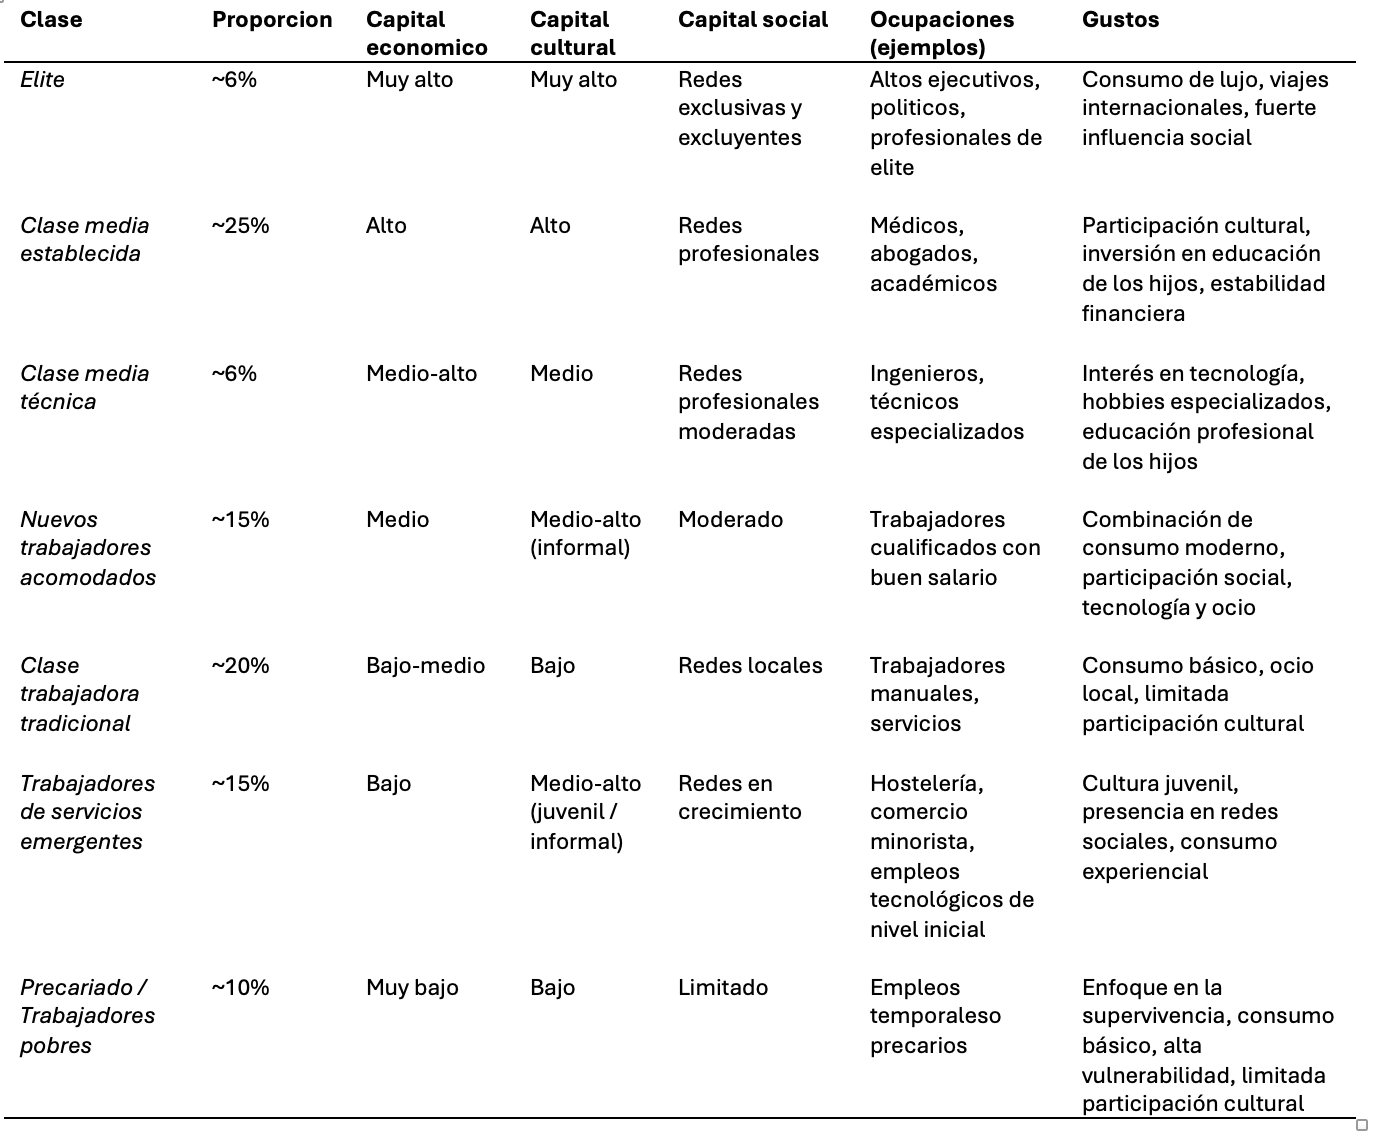
\includegraphics[keepaspectratio]{images/clasesocial.png}}

}

\caption{Tipologia de clases sociales (Savage, 2015)}

\end{figure}%

\subsection{Clase como práctica y experiencia institucional: Willis y la
reproducción cultural del
control}\label{clase-como-pruxe1ctica-y-experiencia-institucional-willis-y-la-reproducciuxf3n-cultural-del-control}

Otro autor también relevante, y un clásico en el estudio de la clase
social, es el británico Paul Willis (1977). Willis aportó una lectura
etnográfica de cómo la clase se reproduce a través de la cultura
institucional. En \emph{Learning to Labour}, Willis observó a un grupo
de jóvenes de clase obrera en una escuela inglesa, mostrando cómo su
resistencia frente a la autoridad escolar ---expresada en burlas,
ausencias y rechazo al esfuerzo académico--- se transformaba
paradójicamente en un mecanismo de reproducción de su posición social.
Los ``lads'' (``los chavales'') rechazaban la cultura escolar burguesa y
reivindicaban valores de masculinidad obrera y autonomía, pero esa misma
resistencia los conducía a aceptar empleos manuales precarios,
perpetuando el destino de clase de sus padres.

El aporte teórico de Willis es util para complementar la aportación de
Bourdieu: mientras el francés describe el proceso de interiorización de
las estructuras sociales en el habitus, Willis muestra cómo se
construyen y reafirman esos habitus dentro de instituciones concretas,
mediante prácticas de resistencia y significación. Las instituciones,
lejos de ser meros instrumentos de reproducción, son espacios activos
donde se produce la identidad de clase. La escuela, la fábrica o la
prisión son lugares donde los individuos aprenden no solo competencias,
sino quiénes son y qué lugar ocupan en el mundo social.

Esta lectura institucional y cultural de la clase ha sido extendida al
campo penal por autores como Loïc Wacquant (2009), discípulo directo de
Bourdieu. En \emph{Punishing the Poor}, Wacquant argumenta que las
instituciones del control penal en las sociedades neoliberales funcionan
como mecanismos de producción de la marginalidad de clase. La prisión,
el gueto y el mercado laboral precario forman un sistema
interdependiente que define, controla y estigmatiza a las clases
subordinadas. El encarcelamiento masivo, especialmente de hombres
jóvenes de clases trabajadoras y minorías étnicas, no responde a una
mayor criminalidad, sino a una política de gestión del excedente social.

Para Wacquant, la prisión ---junto con los guetos urbanos y los mercados
laborales precarios (Wacquant 2008)--- constituyen una red institucional
que reproduce la marginalidad, definiendo a los sectores subordinados
como peligrosos, incapaces o moralmente defectuosos. En esta
perspectiva, la cárcel cumple una función similar a la que Willis
atribuía a la escuela: inculcar en los individuos un sentido práctico de
los límites sociales, una interiorización de su posición subordinada
dentro del orden de clase.

Esta idea conecta directamente con la noción de ``instituciones
totales'' desarrollada por Erving Ervin Goffman (1961). Tanto las
cárceles como los manicomios, reformatorios o cuarteles imponen una
ruptura entre el individuo y el mundo exterior, reorganizando su
identidad en función de las normas institucionales. En el caso de las
clases populares, la exposición reiterada a estas instituciones ---ya
sea en la escuela, los servicios sociales o el sistema penal--- produce
una trayectoria institucional acumulativa que configura la subjetividad
de los sujetos como ``casos'', ``usuarios'' o ``internos''. De este
modo, las instituciones de control social no solo disciplinan conductas,
sino que constituyen identidades de clase (Wacquant 2009).

Así, tanto Willis como Wacquant permiten entender la clase no solo como
una posición o un habitus, sino como una experiencia
\textbf{institucionalmente producida}. La exposición reiterada a
instituciones disciplinarias ---la escuela, los servicios sociales, la
policía, la prisión--- activamente forja habitus de subordinación o
resistencia que reafirman las fronteras sociales. En este sentido, las
instituciones de control son constitutivas de la clase: definen las
trayectorias posibles, los lenguajes legítimos y las identidades
viables.

Desde Marx hasta Wacquant, la teoría de la clase ha transitado de la
estructura económica a la práctica social. Hoy, comprender la relación
entre clase y delito exige asumir que la clase no es solo una categoría
objetiva, sino también un modo de vida y una posición institucionalmente
fabricada. En ese sentido, las desigualdades penales no son únicamente
reflejo de diferencias económicas, sino resultado de cómo las
instituciones ---educativas, laborales, policiales y judiciales---
enseñan a los individuos su lugar en el orden social. Esta concepción
amplia de clase social será clave para analizar, en la siguiente
sección, cómo se distribuyen empíricamente el delito y la sanción en las
sociedades contemporáneas.

\begin{tcolorbox}[enhanced jigsaw, bottomtitle=1mm, toprule=.15mm, colbacktitle=quarto-callout-note-color!10!white, bottomrule=.15mm, leftrule=.75mm, colframe=quarto-callout-note-color-frame, opacitybacktitle=0.6, titlerule=0mm, breakable, colback=white, left=2mm, arc=.35mm, title=\textcolor{quarto-callout-note-color}{\faInfo}\hspace{0.5em}{Nota}, toptitle=1mm, coltitle=black, rightrule=.15mm, opacityback=0]

\textbf{Philippe Bourgois: clase, violencia simbólica y criminalización
en la vida cotidiana}

El trabajo etnográfico de Philippe Bourgois (1995) ofrece una
ilustración empírica de cómo las distintas dimensiones teóricas de la
clase que hemos visto ---estructural, simbólica, moral y afectiva---
convergen en la vida cotidiana de las poblaciones marginalizadas. Su
obra puede leerse como un puente entre los análisis estructurales del
capitalismo y del Estado, las teorías del habitus y la reproducción
simbólica, las perspectivas culturales sobre la resistencia de clase y
las críticas feministas sobre la moralidad y el valor social.

En \emph{In Search of Respect: Selling Crack in El Barrio} (1995),
Bourgois realiza un trabajo de campo etnográfico en el East Harlem de
Nueva York, donde estudió la economía informal del narcomenudeo del
crack y las formas de vida de los jóvenes puertorriqueños excluidos del
mercado laboral formal. Su análisis revelaba cómo la búsqueda de respeto
y dignidad se convierten en una forma de resistencia cultural ante la
humillación estructural, pero también en un mecanismo que reproduce la
exclusión y la criminalización. Los protagonistas de su etnografía
rechazaban los empleos precarios y mal pagados que los sitúan en
posiciones subordinadas, y encontraban en la venta de drogas una fuente
alternativa de estatus, identidad y masculinidad. Sin embargo, esta
forma de afirmación los exponía a la violencia policial, al
encarcelamiento y al deterioro físico y emocional.

Bourgois interpreta este proceso como una manifestación de lo que
Bourdieu denominó violencia simbólica: la internalización de las
jerarquías sociales en forma de culpa, vergüenza y autodesprecio. Los
individuos aprendían a atribuir sus fracasos a su propio carácter o a
decisiones personales, sin reconocer que estaban inscritos en una
estructura de dominación racial y de clase. Esta violencia simbólica se
traduce, en la práctica, en lo que Bourgois llama una ``búsqueda de
respeto'': un intento desesperado por reconstruir valor personal en un
entorno que constantemente lo niega.

Al mismo tiempo, su trabajo muestra que la resistencia cultural descrita
por Willis (1977) y la construcción moral del valor analizada por Skeggs
(1997) están íntimamente entrelazadas. En \emph{El Barrio} (la zona que
estudió), la masculinidad obrera se expresa a través de la fuerza, la
lealtad y la autonomía ---formas de ``respetabilidad'' alternativas al
ideal burgués---, pero estas estrategias están atravesadas por la
precariedad y la violencia. La ``cultura callejera'' no es una simple
oposición al orden dominante, sino una traducción cultural del
sufrimiento estructural.

En investigaciones posteriores, como \emph{Righteous Dopefiend}
(Bourgois y Schonberg 2009), el autor amplía esta mirada al estudiar a
personas sin hogar y usuarias de heroína en San Francisco. Allí
desarrolla el concepto de ``apartheid íntimo'', una forma de segregación
cotidiana que reproduce las jerarquías raciales y de clase incluso
dentro de los márgenes de la pobreza. Mediante la etnografía visual y
participativa, Bourgois y Schonberg documentaron cómo la violencia
estructural ---el abandono estatal, la falta de vivienda, la
precarización del trabajo--- se entrelaza con la violencia simbólica,
generando una vida marcada por la adicción, la represión y el estigma.

Bourgois, por tanto, nos permite ver cómo las teorías de la clase como
estructura (Marx), como habitus (Bourdieu), como frontera moral (Skeggs)
y como cultura de resistencia (Willis) se condensan en la experiencia
concreta del control penal. Su obra evidencia que la criminalización no
es una simple respuesta al delito, sino un mecanismo de gestión del
sufrimiento social, donde las instituciones penales y de bienestar
actúan conjuntamente para producir y administrar la marginalidad. En
este sentido, Bourgois nos ofrece una síntesis empírica que muestra cómo
la clase, la moralidad, la violencia y la criminalización forman parte
de un mismo proceso de reproducción social en las sociedades
contemporáneas y, por tanto, constituye un trabajo de obligada lectura
para los y las criminologas.

\end{tcolorbox}

\section{Clase social, concentración de la riqueza y movilidad social en
España}\label{clase-social-concentraciuxf3n-de-la-riqueza-y-movilidad-social-en-espauxf1a}

Aunque es probable que en las asignaturas de introducción a la
sociología se os den unas nociones más avanzadas de estratificación
social en España, convendría que tuvierais, a efectos de contextualizar
los contenidos de este capítulo, una visión resumida del estado de la
cuestión en nuestro país. Hay toda una serie de fuentes e informes que
ofrecen datos relevantes al respecto (Eurostat, OCDE, CIS, FOESSA, Banco
de España, etc.).

Estas fuentes nos permiten afirmar que España se dibuja como una
sociedad postindustrial, dominada por los servicios, con: una clase
media numerosa pero dualizada; una clase trabajadora en declive, pero
significativa, que ahora se dedica principalmente a los servicios; un
precariado en crecimiento (con fuerte presencia de mujeres, jóvenes e
inmigrantes); una clase alta concentrada en una pequeña élite
empresarial y financiera y ubicada geograficamente en las grandes
capitales. Es un país, además, con desigualdades muy consolidadas
(tenemos baja movilidad social según los estándares de la UE) y fuertes
(y crecientes) desigualdades en materia de vivienda y riqueza, que ahora
superan a las desigualdades de ingresos (que además son particularmente
bajos cuando comparados en terminos reales con la media europea y que se
mantienen estancados en dichos terminos reales). Todo esto constituye un
terreno abonado para que, a la luz de lo visto en la sección anterios y
también a continuación, el sistema de justicia penal tenga que tomarse
muy en serio su papel en cuanto que generador de desigualdades y
exclusión social.

Por lo que respecta a estratificación social, si aplicaramos el esquema
EGP introducido en la sección de interior veríamos que:

\begin{quote}
``aparece una amplia base poblada por los trabajadores en los servicios
(22\%) (donde sobresalen las mujeres nativas e inmigrantes respecto de
los hombres) y las ocupaciones de cualificación elemental (13\%). Y una
cúspide dirigente y tecnocrática compuesta por un 19\% de profesiones
técnico-científicas, más un 4\% de directores y gerentes. Luego
encontramos en un nivel intermedio a los técnicos de apoyo (11\%) y los
empleos administrativos (10\%), y por fin, la clase obrera industrial
compuesta por trabajadores cualificados de la manufactura y operadores
(19\%).'' (Fundación Foessa" 2025, 49)
\end{quote}

Una de las características de la estructura social española es, como
hemos apuntado, su dualizado mercado laboral, con trabajadores de
primera y segunda división:

\begin{itemize}
\item
  Insiders: trabajadores estables, a menudo del sector público;
  protegidos por contratos indefinidos.
\item
  Outsiders: trabajadores temporales y precarios con escasas
  perspectivas profesionales.
\end{itemize}

Esta dualidad afecta a todas las clases sociales, pero golpea con mayor
dureza a la clase media baja y a la clase trabajadora. Es de recalcar
que el empleo temporal ha sido historicamente muy alto, entre los más
altos de la UE. No obstante, las reformas introducidas en las ultimas
legislaturas (combinación de restricciones en el uso de contratos
temporales, junto con el impulso de los fijos discontinuos para
canalizar trabajos que se desarrollan de forma intermitente pero
recurrente), ha contribuido a la reducción de la tasa de temporalidad
(desde valores superiores al 26\% en 2019 a valores en torno al 15\%
hoy, aun por encima del 12\% de media en Europa).

Por otro lado, en España la ``clase trabajadora'' en España se encuentra
ahora: altamente basada en los servicios; joven, migrante y feminizada;
y concentrada en la hostelería, el turismo, el cuidado de personas
mayores, los trabajos esporádicos, el comercio minorista y la logística
(Fundación Foessa" 2025).

Aunque la sociología durante mucho tiempo se obsesionó con tan solo las
desigualdades en materia de ingresos, hay una amplia línea de
investigación que destaca ahora la mayor relevancia de las desigualdades
en materia de riqueza (Piketty 2021). En este sentido, España se ha
convertido también en uno de los países donde la desigualdad de riqueza
importa más que la desigualdad de ingresos. En España la propiedad
inmobiliaria es clave en este sentido y las principales divisiones se
establecen entre propietarios frente a inquilinos, propietarios de
múltiples inmuebles frente a propietarios de una sola vivienda, y
cohortes (generaciones) más jóvenes que se encuentran excluidas de la
propiedad. En nuestro país, no es exagerado decir que la riqueza
inmobiliaria es el principal mecanismo de reproducción intergeneracional
de clases (Barceló et~al. 2025; Fundación Foessa" 2025).

Como ocurre en otros países, también se observa en España una
concentración de la riqueza en la parte superior de la ``piramide''
social. Los datos de la Encuesta Financiera de las Familias del Banco de
España sugieren que entre 2011 y 2021, la proporción de riqueza neta en
manos del 5\% de los hogares más ricos aumentó en aproximadamente 7,3
puntos porcentuales. En otras palabras, los ricos cada vez se comen una
mayor parte del pastel. Según el Atlas de la Riqueza en España, el 1\%
más rico de los españoles posee alrededor del 26-27\% de la riqueza
total, mientras que el 10\% más rico posee casi el 60\% (Marrero et~al.
2025). Esta es ademas una concentración con importantes dimensiones
generacionales: la brecha económica entre las personas de 65 años y las
de 35 se ha duplicado y ahora se asemeja a la de Estados Unidos (Oficina
Nacional de Prospectiva y Estrategia del Gobierno de España 2021). Una
alta concentración de riqueza significa que un menor número de hogares
controla una gran parte de los recursos, lo que afecta al poder
económico, la influencia política y la movilidad intergeneracional. Esto
implica que la clase social y las oportunidades en la vida están cada
vez más vinculadas a la posesión de activos, y no solo a los ingresos.

Visto lo anterior no debería sorprender que España se posicione como un
país con niveles absolutos de movilidad social que son bajos en términos
comparados. Los informes comparativos de la OCDE (2018) muestran que
España se sitúa en la mitad baja de Europa en movilidad de ingresos. En
el informe ``\emph{A Broken Social Elevator?}'', España aparece como un
país donde hacen falta cuatro generaciones para que los descendientes de
familias pobres alcancen el ingreso medio, frente a dos o tres en países
más móviles. La movilidad es mayor en comunidades autónomas y provincias
con mercados laborales diversificados (Madrid, País Vasco, Cataluña) y
sistemas educativos más inclusivos. Y es menor en regiones con alto paro
estructural (Andalucía, Extremadura) y tasas elevadas de empleo
temporal.

Tenemos, finalmente, un país en el que la pobreza es más consistente y
crónica y en el que la privación material crece a pesar del crecimiento
económico; en el que los ingresos de los hogares más vulnerables se han
vuelto más inestables; en el que una educación cada vez más privatizada
y dualizada contribuye a acentuar, en lugar de limar, las diferencias
sociales; y en el que persisten marcados patrones territoriales de
desigualdad y pobreza entre distintas regiones y dentro de las ciudades
(Fundación Foessa" 2025). Con esta fotografía muy resumida podemos en la
siguiente sección aproximarnos de una forma más informada y
contextualizada a lo que la investigación empírica, sobre todo fuera de
nuestras fronteras, ha contribuido al estudio de la relación entre clase
social, delincuencia y actuaciones del sistema de justicia penal.

\section{Investigación empírica: clase y delito en el siglo
XX}\label{investigaciuxf3n-empuxedrica-clase-y-delito-en-el-siglo-xx}

Una muy buena parte de los estudios, sobre todo de caracter
cuantitativo, en criminología han estado orientados a tratar de
discernir si existe una correlación entre clase social y delincuencia. A
lo largo del siglo XX, esta investigación empírica sobre la relación
entre clase social y criminalidad ha oscilado entre dos polos: por un
lado, la evidencia de las estadísticas oficiales, que muestran una
sobrerrepresentación persistente de las clases trabajadoras en los
registros policiales y penitenciarios; por otro, los resultados de los
estudios de autoinforme, que han cuestionado la magnitud real de esas
diferencias. Este contraste metodológico ha generado uno de los debates
más duraderos de la criminología moderna: ¿las clases bajas cometen
realmente más delitos, o simplemente son más visibles para las agencias
de control social?

A este debate se le han ido añadiendo capas. Así, durante los años 1970
se empezó a investigar si había también una relacion entre clase social
y victimación, si las poblaciones socialmente más vulnerables están
también más expuestas al delito. Y el enfasis de las teorías del
etiquetamiento llevó a consolidar líneas de investigación sobre el
impacto en estatus socioeconómico del etiquetado o la intervencion
penal. Finalmente, también ha habido estudios que en lugar de estudiar
la relacion entre clase social, en un sentido estático, y delincuencia
han estudiado la relacion entre movilidad social y delincuencia. En este
apartado del capítulo delinearemos que es lo que hemos aprendido desde
todas estas perspectivas.

\subsection{Las estadísticas oficiales y la construcción de vínculos
entre clase y
delincuencia}\label{las-estaduxedsticas-oficiales-y-la-construcciuxf3n-de-vuxednculos-entre-clase-y-delincuencia}

La criminología empírica temprana, especialmente en Europa y Estados
Unidos, se basaba casi exclusivamente en las estadísticas oficiales
sobre delincuencia recopiladas por la policía, la administración de
justicia, y las prisiones. Estos datos mostraban sistemáticamente que
los delincuentes procedían de manera desproporcionada de entornos
socioeconómicos más bajos. Estudios de principios del siglo XX en Gran
Bretaña (por ejemplo, Goring (1913)) sugerían que las personas con
ocupaciones no cualificadas o manuales estaban muy sobrerrepresentadas
entre los condenados penales y la población carcelaria.

No debería sorprender, por tanto, que desde los primeros estudios
sociológicos, la asociación entre desventaja social y delincuencia fuera
asumida como un hecho empírico. Las investigaciones de la Escuela de
Chicago, en particular \emph{Juvenile Delinquency and Urban Areas} (Shaw
y McKay 1942), mostraron que las tasas de delincuencia juvenil
registradas en estadísticas oficiales se concentraban en zonas urbanas
empobrecidas caracterizadas por altos niveles de desorganización social,
movilidad residencial y heterogeneidad étnica. Sin embargo, los autores
subrayaron que la pobreza en sí misma no causaba el delito, sino que
generaba contextos donde las instituciones de control informal eran más
débiles y donde se transmitían subculturas tolerantes con la desviación.
Esta observación consolidó la idea de que las condiciones estructurales
de los barrios obreros influían en la transmisión intergeneracional del
comportamiento delictivo.

Sin embargo, es importante remarcar que estos patrones de correlación
deben interpretarse en el contexto del sesgo institucional y las
prácticas estatales de control social. Como hemos insistido, desde
finales del siglo XIX, los sistemas policiales y penales de las
sociedades industriales se centraron de manera desproporcionada en la
clase trabajadora urbana, los vagabundos y otros grupos marginados. Por
lo tanto, los datos oficiales reflejaban, y hoy también siguen
reflejando, no solo los patrones de comportamiento, sino también la
selectividad de las instituciones de justicia penal, que daban prioridad
a la vigilancia y el castigo de los pobres.

\subsection{Los estudios de autoinforme y el mito de la relación con
clase
social}\label{los-estudios-de-autoinforme-y-el-mito-de-la-relaciuxf3n-con-clase-social}

La correlación entre clase social y delincuencia, como acabamos de ver
respaldada por los primeros estudios que utilizaban estadísticas
oficiales sobre delincuencia, fue profundamente cuestionada por la
aparición de las encuestas de autoinforme a mediados del siglo XX, que a
menudo encontraban una correlación débil o inexistente. Durante la
segunda mitad del siglo XX, los estudios británicos y estadounidenses
basados en autoinformes ofrecieron una visión más matizada sobre la
relacion entre clase social y delincuencia. A diferencia de las
estadísticas oficiales basadas en detenciones y condenas, estas
encuestas preguntaban directamente a las personas sobre su participación
en actos delictivos.

Investigaciones pioneras como las de Porterfield (1946) revelaron que
los niveles de implicación en comportamientos delictivos leves
(vandalismo, hurtos menores, consumo de drogas) eran relativamente altos
en todas las clases sociales, especialmente durante la adolescencia. No
obstante, las diferencias surgían en las consecuencias: los jóvenes de
clase trabajadora eran mucho más propensos a ser detenidos o etiquetados
como ``delincuentes'' por la policía.

Esta discrepancia provocó una reevaluación crítica de las
investigaciones que habían respaldado la visión tradicional. Tittle y
Villemez (1977) identificaron numerosas deficiencias metodológicas en la
bibliografía existente que, basándose en datos oficiales, encontraba una
correlación entre clase social y delincuencia:

\begin{itemize}
\item
  \emph{Falacia ecológica}: muchos estudios citados con frecuencia
  ofrecían correlaciones para áreas ecológicas en lugar de para
  individuos, lo que hacía imposible concluir que los individuos de
  clase baja de esas áreas fueran los que cometían delitos. Que en
  barrios más pobres haya más delincuencia (una relación a nivel meso o
  ecológico), no significa que las personas más pobres cometan más
  delitos (una relación a nivel individual).
\item
  \emph{Proxies deficientes}: algunos estudios importantes utilizaban
  las características de los distritos censales (por ejemplo, la renta
  media) como proxy (medida aproximada) del estado familiar de un
  individuo, lo que no es una medida fiable.
\item
  \emph{Medidas rudimentarias}: La investigación se vio a menudo
  debilitada por medidas rudimentarias de la clase social o del tipo y
  la gravedad de los delitos.
\item
  \emph{Muestras limitadas}: Muchos estudios se limitaron a una sola
  categoría racial o sexual (por ejemplo, hombres blancos), lo que
  limitó su generalización.
\end{itemize}

Basándose en sus trabajos anteriores, Tittle, Villemez, y Smith (1978),
llevaron a cabo lo que describieron como una ``evaluación empírica de la
evidencia empírica'' para resolver el estado caótico y contradictorio de
la literatura. Identificaron 35 estudios y redujeron los resultados a
363 medidas comparables de asociación (coeficientes gamma), que luego
analizaron para identificar patrones sistemáticos. Su conclusión
principal fue que la relación entre la clase social y la criminalidad
era un ``mito''. La media general gamma en los 363 casos fue de -0,09,
una cifra que indica que casi no existe relación. Sin embargo, su
análisis multivariante reveló dos variables cruciales que explicaban
gran parte de la variación en los resultados del estudio: el tipo de
datos utilizados y la década en la que se realizó el estudio.

Sin embargo, investigaciones posteriores demostraron que esta conclusión
era prematura. La declaración de que la correlación entre clase social y
delincuencia era un ``mito'' fue inmediatamente cuestionada. Los
críticos argumentaron que la conclusión era prematura y se basaba en un
conjunto de investigaciones incompletas y metodológicamente defectuosas.
Por ejemplo, un estudio realizado por Farnworth et~al. (1994)
argumentaba que los resultados débiles e inconsistentes de la
bibliografía se debían a un ``vacío teórico'' en la forma de medir la
clase social y la delincuencia.

Estudios de autoinforme metodológicamente mejorados, como la
\emph{National Youth Survey} analizada por Elliott y Ageton (1980),
revelaron que sí existen diferencias significativas entre clases,
especialmente en lo que respecta a los delitos graves. La discrepancia
se explicó por el hecho de que los estudios anteriores no habían tenido
en cuenta los delitos de alta frecuencia, que se concentran más entre
los jóvenes de clase baja.

Investigaciones posteriores han refinado los enfoques de medición,
demostrando que la fuerza de la relación depende en gran medida de cómo
se miden tanto la clase como la delincuencia. La correlación es más
evidente cuando la clase social se define como una situación de subclase
persistente (por ejemplo, desempleo de larga duración, dependencia de
las ayudas sociales) y el delito se mide como delitos graves o
frecuentes. Este vínculo persiste incluso en los estados del bienestar
nórdicos, caracterizados por su igualitarismo.

\subsection{El continuado sesgo del sistema de justicia
penal}\label{el-continuado-sesgo-del-sistema-de-justicia-penal}

Al margen de conducir a un mayor refinamiento en el estudio de la
relación entre clase social y delincuencia, los estudios de autoinforme
también contribuyeron a animar investigaciones orientadas a preguntarse
si la relación encontrada es, al menos parcialmente, el fruto de los
propios sesgos del sistema de justicia penal. La correlación entre la
clase social y las diferencias en la actuación policial y las sentencias
está, en la actualidad, bien documentada: un estatus socioeconómico más
bajo se asocia sistemáticamente con una actuación policial y sentencias
más severas, lo que a menudo se combina con la raza y el origen étnico
para amplificar las disparidades.

Los resultados de estos estudios demuestran colectivamente que las
disparidades en la actuación policial, el enjuiciamiento y el castigo no
son simplemente el resultado de prejuicios aislados y episódicos. Por el
contrario, están profundamente arraigadas y son producto de estructuras
sociales más amplias, procesos acumulativos que se desarrollan a lo
largo de la vida y profundos cambios sociales que remodelan el panorama
de la delincuencia y la justicia para generaciones enteras.

La literatura académica especializada menciona tres mecanismos que
explican estos vínculos:

\begin{itemize}
\item
  \emph{Actuación policial excesiva en comunidades desfavorecidas}: la
  policía tiende a centrarse y desplegar recursos en barrios con altos
  índices de pobreza y desventaja social, lo que aumenta la probabilidad
  de que las personas de clase baja entren en contacto con las fuerzas
  del ``orden'' y sean detenidas (Sampson 1986). Los agentes de policía
  son además significativamente más propensos a utilizar niveles más
  altos de fuerza cuando se enfrentan a sospechosos en barrios
  desfavorecidos (Terrill y Reisig 2003). Es predominantemente hombres
  pobres y de baja condición social quienes ocupan una posición central
  en la carga de trabajo práctico de la policía y en su conciencia
  ocupacional (Loftus 2007). ¿Por qué? En parte porque la policía tiende
  a asociar ciertas áreas geográficas con ``lugares sospechosos'' o
  ``lugares problemáticos''. Esto conduce al fenómeno de la
  ``\emph{contaminación ecológica}'', en el que las personas que se
  encuentran en barrios considerados ``malos'' son vistas como
  portadoras de la responsabilidad moral del propio barrio, lo que
  aumenta su vulnerabilidad a la coacción (Werthman y Piliavin 1967). De
  ahí que se afirme que la policía no solo ejerce una función técnica de
  control del delito, sino que es una poderosa fuerza política y social
  que moldea activamente las fronteras entre grupos, el significado
  social y la experiencia de la ciudadanía. Los distintos grupos
  minoritarios suelen sufrir una combinación única de exceso de
  vigilancia policial (aplicación excesiva e injusta de la ley) y falta
  de vigilancia policial (negligencia e incapacidad para garantizar la
  seguridad).
\item
  \emph{Discriminación en las sentencias}: El contexto socioeconómico
  influye en las decisiones judiciales, y la privación social a menudo
  no se reconoce como un factor atenuante, lo que da lugar a sentencias
  más severas para los acusados más pobres. El entorno en el que se
  administra la justicia es un factor determinante de sus resultados.
  Las investigaciones indican que las características a nivel
  comunitario (entre ellas, la desigualdad económica, la composición
  racial y la privación social) no solo constituyen un telón de fondo
  pasivo, sino que influyen activamente en las decisiones sobre las
  sentencias, a menudo interactuando con la raza y la condición social
  del delincuente (Myers 1987; Donnelly 2022; Pina-Sanchez et~al. 2022).
  Como señala Sampson y Loeffler (2010) (p.~21):
\end{itemize}

\begin{quote}
``Los puntos donde se concentra el encarcelamiento no son aleatorios;
por el contrario, se predicen sistemáticamente a partir de
características sociales clave. En particular, la combinación de
pobreza, desempleo, desintegración familiar y aislamiento racial está
ligada a altos niveles de encarcelamiento, incluso cuando se ajusta la
tasa de delincuencia que experimenta una comunidad.''
\end{quote}

\begin{itemize}
\tightlist
\item
  \emph{Desventaja acumulativa}: La desventaja acumulativa es distinta
  de la simple disparidad episódica. Se refiere a un proceso en el que
  los acontecimientos o situaciones negativas tempranas desencadenan
  efectos en cadena, magnificando las diferencias preexistentes y
  produciendo desigualdades cada vez mayores con el paso del tiempo
  (Kurlycheck y Johnson 2019). El concepto abarca tanto un crecimiento
  exponencial de la desigualdad a lo largo del tiempo (el «efecto
  Mateo») como un proceso aditivo en el que múltiples estatus (por
  ejemplo, raza, clase, género) interactúan para producir resultados
  negativos compuestos. Basándose en la teoría del etiquetado y en las
  perspectivas del ciclo vital, la desventaja acumulativa postula que el
  contacto temprano con el sistema judicial puede servir como un «punto
  de inflexión» negativo, creando impedimentos estructurales,
  debilitando los vínculos sociales y limitando las oportunidades
  futuras, lo que aumenta la probabilidad de cometer delitos y recibir
  castigos en el futuro. Las desventajas se agravan a lo largo del
  proceso de justicia penal: la vigilancia policial excesiva da lugar a
  más detenciones, lo que a su vez aumenta la probabilidad de que las
  personas de clase baja sean objeto de un enjuiciamiento y una
  sentencia severos. La desventaja también se agrava a medida que el
  caso avanza en el sistema judicial, y las reformas que se centran en
  solventar problemas de disparidad en una etapa pueden simplemente
  desplazar la discrecionalidad y la disparidad a otra. Sabemos ademas
  que las decisiones tempranas tienen poderosos efectos posteriores. Por
  ejemplo, múltiples estudios demuestran que la detención preventiva
  aumenta significativamente las probabilidades de condena y de una
  sentencia final más severa. Dado que los acusados pertenecientes a
  minorías y con bajos recursos económicos son más propensos a ser
  detenidos, esto se convierte en un mecanismo clave para la desventaja
  acumulativa (Kurlycheck y Johnson 2019).
\end{itemize}

\subsection{Castigo penal y clase social: el impacto del sistema de
justicia penal en estatus
socioeconómico}\label{castigo-penal-y-clase-social-el-impacto-del-sistema-de-justicia-penal-en-estatus-socioeconuxf3mico}

Una perspectiva o angulo de investigación adicional surge al examinar la
relacion entre justicia penal y clase social en términos del impacto que
las actuaciones del sistema de justicia penal tienen en la clase social
de los individuos sobre los que se actúa. A diferencia del foco de las
investigaciones anteriores sobre disparidad en función de la clase
social, hay otros estudios que se han centrado en investigar de qué
forma el sistema de justicia penal, a través de sus intervenciones en la
vida de las personas (prioritariamente a traves de las sanciones o los
registros de antecedentes penales), afecta al estatus socioeconómico y
las trayectorias laborales de estas personas. La pregunta que se
plantean estos estudios no es si personas de clase social baja cometen
más delitos (como veiamos en 10.5.1 y 10.5.2) o son más propensos a
recibir interveciones policiales o sanciones más duras (sección 10.5.3),
sino si estas intervenciones del sistema de justicia penal contribuyen a
conformar la clase social de quienes caen bajo sus redes.

Hay ahora un amplio cuerpo de estudios, algunos de los cuales han podido
usar, solidos diseños experimentales, lo que hace más creibles sus
inferencias, sobre esta relación. Sabemos que existe una clara relación
entre las sanciones penales o tener antecedentes penales y un estatus
socioeconómico más bajo, lo que limita directamente la movilidad social.
Las desventajas socioeconómicas no solamente aumentan la probabilidad de
verse involucrado en la justicia penal como vimos en la sección
anterior, sino que también empeoran los efectos negativos sobre las
oportunidades futuras cuando se tienen antecedentes penales. Algunos
estudios incluso documentan graves dificultades materiales
inmediatamente después del encarcelamiento (Western et~al. 2015).

Como hemos visto en la sección anterior, las personas de entornos
socioeconómicos más desfavorecidos son más propensas a recibir penas más
severas, en parte porque disponen de menos recursos para desenvolverse
en el sistema, como la fianza o la representación legal efectiva. Pero
además una vez enredados en el sistema, las consecuencias negativas de
las sanciones agravan las desventajas socioeconómicas pre-existentes,
perpetuando aún más los ciclos de pobreza y limitando el acceso a la
educación, el empleo y la vivienda.

Las investigaciones demuestran sistemáticamente que las personas con
antecedentes penales o que han sido objeto de sanciones penales se
enfrentan a importantes obstáculos para acceder al empleo, la vivienda y
la participación social, lo que a su vez restringe la movilidad social y
refuerza las desventajas socioeconómicas (Craigie, Grawert, y Kimble
2020; Corda, Rovira, y Henley 2023; Bryant 2025). Estos efectos no solo
son inmediatos, sino que pueden persistir durante décadas, afectando a
los resultados del mercado laboral y a la inclusión social hasta bien
entrada la edad adulta (Maroto 2015).

Sabemos que el encarcelamiento tiene efectos negativos profundos y
duraderos tanto en los ingresos a lo largo de la vida como en las
perspectivas de empleo futuras. Estas consecuencias persisten durante
años después de la puesta en libertad y pueden alterar drásticamente la
trayectoria financiera de una persona. Tener antecedentes penales limita
mucho las posibilidades de ascender socialmente porque dificulta el
acceso a trabajos, licencias profesionales y oportunidades educativas, y
crea un estigma social (Larrauri 2014; Rovira 2019). Las personas que
han estado en prisión se enfrentan a obstáculos mucho mayores a la hora
de encontrar y mantener un empleo; su tasa de desempleo es casi cinco
veces superior a la de la población general. Algunos estudios sugieren
que quienes han estado encarcelados pasan entre 0,8 y 4,2 años más sin
trabajo (Gordon y Neelakantan 2021). Estas barreras afectan la
estabilidad económica a largo plazo y pueden generar pobreza
multigeneracional.

Las investigaciones demuestran de forma reiterada que el encarcelamiento
conduce a una disminución prácticamente permanente de los ingresos
(Craigie, Grawert, y Kimble 2020). Por ejemplo, los hombres que son
encarcelados por primera vez experimentan una reducción del 33 al 50 \%
en sus ingresos a lo largo de la vida en comparación con personas
similares que nunca han estado en prisión (Gordon y Neelakantan 2021).
El encarcelamiento puede hacer que una condena de un año reduzca los
ingresos acumulados en un 13 \% durante los cinco años siguientes (Garin
et~al. 2024). Tras su puesta en libertad, los ingresos medios de los
exreclusos son considerablemente más bajos: en el primer año tras su
puesta en libertad, solo el 55 \% declaró ingresos legales, con una
mediana de apenas 10 090 dólares (Looney 2018).

El impacto de estos efectos no es homogeneo. Algunos penados lo sufren
más que otros. Por ejemplo, sabemos que el encarcelamiento en una etapa
temprana de la vida tiene repercusiones especialmente graves: interrumpe
los años clave para la construcción de una carrera profesional, lo que
dificulta mucho más que las personas puedan ponerse al nivel de sus
compañeros en términos de ingresos o desarrollo profesional (Emmert
2020). También sabemos que las personas que han sido encarceladas en
múltiples ocasiones sufren déficits aún más significativos en materia de
empleo y ingresos a largo plazo que aquellas que solo han sido
encarceladas una vez (Craigie, Grawert, y Kimble 2020). Por otra parte,
las personas que parten de una situación socioeconómica más favorecida
también se ven afectadas, pero las investigaciones sugieren que las
personas de entornos desfavorecidos se enfrentan a obstáculos más
duraderos para ``corregir el rumbo'', lo que significa que les resulta
más difícil escapar de la desventaja tras el estigma o el castigo.

El sesgo del sistema de justicia penal contra minorías étnicas también
es relevante en este sentido. Estudios realizados en Estados Unidos
muestran que debido a que el encarcelamiento de las minorias es tan
frecuente, el efecto del encarcelamiento sobre los salarios individuales
también aumenta la desigualdad salarial agregada por raza y etnia
(Western 2002). Estudios también conducidos en Estados Unidos sugieren
que:

\begin{quote}
``los afroamericanos y los hispanos tienen ingresos totales inferiores a
los de los blancos, incluso después de tener en cuenta la salud, el
capital humano, el origen social, la delincuencia y la implicación en la
justicia penal, y la preparación para el empleo. Un desglose atribuye la
mayor parte de las diferencias salariales a las desigualdades raciales y
étnicas en el empleo. Las entrevistas cualitativas sugieren que los
blancos, más que los afroamericanos y los hispanos, encuentran trabajos
estables y bien remunerados a través de las redes sociales.'' (Western y
Sirois 2019, 1517)
\end{quote}

Aunque la mayoría de los estudios más solidos se han desarrollado en
Estados Unidos, el impacto negativo de los antecedentes penales en los
resultados socioeconómicos se observa en muchos países y contextos
(Pager 2003). Incluso en lugares con menos restricciones formales (como
algunos países de Europa), las barreras informales ---como el rechazo de
los empleadores a contratar a personas con antecedentes--- siguen
reduciendo drásticamente las oportunidades (Corda, Rovira, y Henley
2023). El estigma de tener antecedentes penales, sumado al
debilitamiento de las redes sociales y a la interrupción de la
experiencia laboral, limita las oportunidades de empleo y los salarios,
lo que deja a muchas personas en puestos de trabajo precarios y con
salarios bajos.

Existe en la actualidad también, sobre todo en la literatura
estadounidense, un interes creciente en el analisis de las multas y
otros costes economicos de la involucracion en la justicia penal, y su
impacto diferencial (Martin et~al. 2018). Existe una creciente
convicción entre estos autores de que el sistema de justicia penal
extrae riqueza de las personas pobres a través de multas, tasas y
sanciones, lo que limita aún más su capacidad para mejorar su situación
(Menendez et~al. 2019). Tales obligaciones financieras pueden dar lugar
a la criminalización de la pobreza, en la que la posterior intervención
judicial no se debe a un delito, sino a la incapacidad de hacer frente a
las cargas financieras del proceso judicial (Pager, Goldstein, y Western
2022). Desde esta perspectiva se mantiene que el sistema de justicia
penal se ha adaptado para desviar recursos de los grupos subordinados,
subvencionar a los gobiernos y generar beneficios empresariales a través
de una amplia gama de prácticas. En un contexto en el que se ha
disminuido la carga fiscal de los más rucism esta extracción financiera
se considera que viene a agravar mas las desigualdades e injusticias
raciales y de clase (Page y Soss 2025).

Las sanciones penales y los antecedentes penales, por tanto, están
estrechamente relacionados con un nivel socioeconómico más bajo y una
menor movilidad social, y hay pruebas que demuestran que estos efectos
son tanto causa como consecuencia de la desigualdad social.

\subsection{Victimación y clase
social}\label{victimaciuxf3n-y-clase-social}

A partir de la década de 1970, la introducción de las encuestas sobre
victimización ---en particular, la Encuesta Británica sobre Delincuencia
(BCS), realizada por primera vez en 1982, y la Encuesta Nacional sobre
Victimización Delictiva (NCVS) de Estados Unidos--- proporcionó una
perspectiva empírica adicional sobre la clase social y la delincuencia.
Estas encuestas demostraron que las personas de clase trabajadora y con
bajos ingresos no solo eran más propensas a ser delincuentes según los
datos oficiales, sino también a ser víctimas de delitos violentos y
contra la propiedad (Sparks, Geen, y Dodd 1977; Hough y Mayhew 1983).

Los análisis de los datos de la BCS a lo largo de los años 80 y 90
confirmaron que los hogares de las zonas urbanas desfavorecidas
experimentaban tasas más altas de robos, agresiones y atracos, incluso
después de controlar los factores demográficos (Kershaw y Tseloni 2005).
Estos resultados reforzaron el argumento de que la clase social
determina tanto la exposición a entornos criminógenos como la
vulnerabilidad a la victimización, algo que estudios posteriores han
venido a confirmar al identificar marcadores de posicion social con
vulnerabilidad a dicha victimación (Tseloni y Pease 2014; Hunter y
Tseloni 2016; Lauritsen 2018) y al acesso diferencial a medidas de
seguridad (Tilley, Tseloni, y Farrell 2011).

Además, los estudios a nivel de barrio, en particular los inspirados en
la tradición ecológica de la Escuela de Chicago, demostraron que la
concentración de la pobreza, la inestabilidad residencial y la baja
eficacia colectiva eran fuertes predictores de las tasas de
victimización (Sampson, Raudenbush y Earls, 1997). Los estudios en esta
linea analizan los datos reconociendo la interaccion entre diferencias
individuales y el contexto social, e ilustran que tanto clase social a
nivel individual, como los contextos ecologicos marginalizados son
relevantes para entender el riesgo de victimización (Lauritsen 2001,
2018; Tseloni 2006).

\subsection{Movilidad social y
delincuencia}\label{movilidad-social-y-delincuencia}

(Sección en desarrollo)

\subsection{Conclusiones sobre la investigación
empírica}\label{conclusiones-sobre-la-investigaciuxf3n-empuxedrica}

A finales del siglo XX, la investigación empírica había , por tanto,
establecido varias conclusiones sólidas. En primer lugar, las personas y
comunidades de clase baja son más propensas a aparecer en las
estadísticas oficiales, pero esto refleja en parte el sesgo policial y
judicial. En segundo lugar, los datos autoinformados y longitudinales
muestran que, si bien la delincuencia menor trasciende las clases
sociales, los delitos persistentes, graves y violentos son más
frecuentes entre las personas que se enfrentan a desventajas sociales y
económicas. En tercer lugar, el riesgo de victimización también está
estructurado por clases: los pobres están más expuestos a delitos
interpersonales y contra la propiedad. El panorama empírico que surgió a
finales del siglo XX confirma así una relación compleja y mediada entre
la clase social y la delincuencia: no es determinista, pero está
profundamente arraigada en las estructuras de oportunidad, marginación y
control estatal.

\section{El delito de cuello blanco}\label{el-delito-de-cuello-blanco}

Uno de los problemas de la criminología tradicional fue su casi
exclusivo foco en el estudio de la llamada ``delincuencia común'' (los
delitos violentos, robos, hurtos, etc.), aquellos delitos generalmente
interpersonales, que constituyeron el grueso de los códigos penales que
fueron legislándose desde el siglo XIX a nuestros días. En la medida en
que los Códigos Penales y el sistema penal fundamentalmente han puesto
el foco de su atención en este tipos de delitos hay que entender que la
mayor parte de los estudios empiricos sobre la relación entre clase
social y delincuencia examinados en la sección anterior en realidad son
estudios sobre la relación entre clase social y ``delincuencia común''.
El problema es que esto implica un sesgo es nuestra forma de mirar a la
realidad criminal.

Este sesgo en la mirada criminológica aún está muy presente. La mayoría
de los estudios criminológicos se centran en este tipo de delitos. Baste
examinar los contenidos de las principales revistas de criminología para
poder concluir que la llamada delincuencia común sigue siendo el
principal objeto de estudio de la criminología. En su análisis
sistemático de los temas cubiertos en revistas criminológicas, Cohn,
Farrington, y Wright (1998) identifican los estudios de la delincuencia
de cuello blanco como el tema menos popular entre los artículos
publicados. Es más, su análisis entre 1986 y 1995 muestra un declive en
interés en esta temática. Como señala (\textbf{Friedrichs\_09?}) (p.~1)
existe, paradójicamente, una relación inversa entre el ``nivel de daño
causado por alguna actividad humana (individual u organizativa) y el
nivel de atención criminológica''. Lynch, McGurrin, y Fenwick (2004)
concluían, en un estudio parecido, que la proporción de contenidos entre
delincuencia común y delincuencia de cuello blanco es de 10 a 1. Y es
precisamente esta observación lo que ha llevado a algunos autores ha
abandonar el marco de la criminología y desarrollar una nueva
disciplina, la zemiología, centrada en el estudio del daño social
(Hillyard y Tombs 2007).

De la situación de la investigación criminológica en España sobre esta
cuestión casi mejor no hablar, porque realmente no hay mucho de lo que
hablar. La única publicación sobre este tema en la \emph{Revista
Española de Investigación Criminológica} es una recensión publicada en
el 2025 en la que se hace una recension de un libro sobre economía
ilícita (y que en buena medida es sobre delincuencia organizada) escrito
por catedrático de sociología (sin vínculos con la \emph{Sociedad
Española de Investigación Criminológica}). No hay, a diferencia de lo
que ocurre con otras temáticas, grupos consolidados de investigación
sobre la delincuencia de cuello blanco en la comunidad criminológica
española.

Reflexionando sobre este abandono, (\textbf{Rothe\_22?}) (p.~1)
consideran que:

\begin{quote}
``La criminología ortodoxa generalmente se identifica a sí misma como
una disciplina científica y tiene un sesgo inherente a favor de las
definiciones de delito que se prestan fácilmente al análisis
cuantitativo. Este sesgo privilegia inevitablemente la atención a las
formas convencionales de delito ---los delitos cometidos por los
desamparados--- que, por su misma naturaleza, se prestan más fácilmente
a la operacionalización. En cierto sentido, entonces, el enfoque de los
criminólogos en la delincuencia callejera refuerza las explicaciones
individuales, racionales e incluso morales de la criminalidad, y al
hacerlo impide cualquier crítica persistente de los acuerdos sociales
existentes.''
\end{quote}

Y, sin embargo, esta mirada comenzó a ser cuestionada precisamente a
través del trabajo pionero de uno de los padres de la criminología
contemporánea cuando Edwin H. Sutherland a partir de la década de los
años 1940, introdujo el concepto del delincuente de cuello blanco. El
estudio de la criminalidad en las clases altas y en las organizaciones
empresariales surgió precisamente como una ruptura deliberada con la
visión tradicional de que el delito era un fenómeno propio de los
sectores marginales. Sutherland (1949) acuñó el concepto de
\textbf{white-collar crime} para referirse a los delitos cometidos por
personas respetables y de alto estatus social en el ejercicio de su
ocupación. De forma específica, Sutherland (1949) (p.9) considera que:

\begin{quote}
``El delito de cuello blanco puede definirse aproximadamente como un
delito cometido por una persona respetable y de alto estatus social en
el ejercicio de su ocupación\ldots{} El término''delito de cuello
blanco'' se utiliza aquí para referirse principalmente a los directivos
y ejecutivos de empresas.''
\end{quote}

Sutherland estaba particularmente preocupado por superar el sesgo de
clase social que observaba en la criminología y en las teorías
criminológicas. Con esta propuesta, Sutherland no solo pretendía
desafiar la imagen popular del delincuente como individuo pobre y
peligroso, sino también la visión predimanente del sistema penal como
una instancia neutra, evidenciando que éste aplica sus sanciones de
forma desigual según la posición social del infractor.

Sutherland (1949) argumentó que las conductas de fraude, manipulación
financiera, soborno o abuso de confianza ---frecuentes en el mundo
empresarial y profesional--- causan daños sociales y económicos mucho
mayores que la delincuencia callejera. Sin embargo, rara vez se las
percibe como delitos. Esto se debe, según él, a un proceso de
diferencial de poder normativo, mediante el cual las clases dominantes
definen qué actos son delictivos y cuáles se consideran
``irregularidades'', ``errores administrativos'' o se regulan como
infracciones del derecho privado o administrativo, en lugar de como
injustos penales. En palabras de Sutherland, la criminalidad de cuello
blanco se oculta tras un velo de respetabilidad que la hace casi
invisible al público y a la justicia penal.

A pesar del caracter innovador de la aportación realizada por Sutherland
(1949), la criminología tardó décadas en aceptar la invitación que
suponía esta aportación para ampliar su mirada. Aunque hubo algunos
estudios inmediatamente posteriores que mantuvieron la llama encendida,
no fue hasta la década de los años 1970 (cuando una serie de casos de
alta relevancia social sacudieron la opinión pública norteamericana) que
otros investigadores sociales empezaron a consolidar el estudio de este
tipo de delitos.

En este período se avanzó en la claridad conceptual. Así, Clinard y
Quinney (1973) distinguieron entre \textbf{ocupational crime} (delitos
ocupacionales) ---cometido por individuos en el marco de su trabajo--- y
\textbf{corporate crime} (delito empresarial) ---cometido en beneficio
de una organización o empresa---, mostrando que ambos tipos de
infracción comparten un patrón de racionalidad económica y bajo riesgo
de sanción. La criminalidad corporativa incluye prácticas como la
contaminación ambiental, la publicidad engañosa, la evasión fiscal, el
fraude financiero o las violaciones a la seguridad laboral. Estas
conductas pueden afectar a miles o millones de personas, pero su
tratamiento judicial suele ser administrativo o civil, no penal (Tombs y
Whyte (2015)).

Una de las contribuciones más significativas de esta línea de
investigación es la idea de que la estructura de poder económico
condiciona el alcance del derecho penal. Chambliss (1975) y Quinney
(1977) sostuvieron que el sistema legal está diseñado para proteger los
intereses de la clase dominante y criminalizar las conductas que
amenazan el orden económico existente. En este sentido, las leyes contra
el hurto o el vandalismo que protegen la propiedad privada son
perseguidas y sancionadas con determinación por el sistema penal,
mientras que las regulaciones sobre el fraude corporativo o los delitos
financieros suelen ser ambiguas o poco aplicadas. La selectividad del
control penal reflejaría, así, la estructura de clases de la sociedad
capitalista.

Diversos escándalos en el contexto europeo (desde el fraude financiero
de Parmalat en Italia hasta el caso Siemens en Alemania o las
manipulaciones de emisiones de Volkswagen) y en el español (el caso
Forum Filatélico, Bankia, Gurtel, Púnica) han puesto de manifiesto la
persistencia y sofisticación del delito corporativo. A pesar del impacto
económico, social y ambiental de estos casos, las sanciones penales
pueden ser leves, y los responsables individuales rara vez enfrentan
prisión. Diversos estudios subrayan que la regulación empresarial en
Europa tiende a priorizar la ``cooperación'' con las corporaciones antes
que la represión, lo que genera un marco de ``autorregulación
controlada'' que perpetúa la impunidad estructural (David Nelken 2012).
Aunque hay organismos y dispositivos reguladores que en teoría deberían
prevenir el delito de cuello blanco y el delito empresarial (Wangman y
Cheng 2016), existe investigación consolidada que demuestra el limitado
impacto que puede tener este tipo de mecanismos, sobre todo por la
``captura'' de los mismos por parte de los sectores regulados, en parte
a traves del proceso de las llamadas puertas giratorias, pero tambien
por el trabajo de lobistas que ejercen su influencia sobre el poder
político para limitar la actividad regulatoria del Estado (Ramirez 2016;
Stănescu 2025).

A nivel empírico, diversas investigaciones han mostrado que el perfil
social de los infractores de cuello blanco difiere notablemente del de
los delincuentes comunes. Generalmente, tienen más edad, un nivel más
elevado de educación, están más integrados socialmente, y están en mejor
situación económica que los delincuentes comunes (Benson, Slyke, y
Cullen 2016). Como resumen Klenowski y Dodson (2016) (p.~102): ``Un
porcentaje considerable de los delincuentes de cuello blanco son hombres
caucásicos de mediana edad con empleos remunerados que suelen cometer su
primer delito de cuello blanco entre los treinta y tantos y los cuarenta
y tantos años''. En ese sentido, Weisburd, Waring, y Chayet (2001)
(p.144) apuntan que los delincuentes de cuello blanco ``son tan
diferentes de otros delincuentes que poco se puede aprender de sus
experiencias sobre el problema más general de la delincuencia''.

En su estudio de cerca de 1000 delincuentes de cuello blanco condenados
por las autoridades federales en Estados Unidos, estos autores
concluyeron que:

\begin{quote}
``La situación desempeña un papel fundamental a la hora de explicar la
participación en delitos de la mayoría de los delincuentes de esta
muestra. Las vidas de aquellos a los que hemos denominado
\emph{oportunistas} y \emph{reactivos ante las crisis} no parecen
caracterizarse por la inestabilidad y la desviación, y hay pocos
indicios en sus antecedentes que apunten a una predisposición a la
delincuencia. De hecho, con frecuencia había pruebas de lo contrario.
Una crisis específica o una oportunidad especial parecen haber empujado
a personas por lo demás convencionales a cruzar la línea hacia la
delincuencia. Incluso en el caso de los descritos como buscadores de
oportunidades, las oportunidades situacionales desempeñan un papel
importante a la hora de definir por qué los delincuentes cometen delitos
en momentos concretos.'' (Weisburd, Waring, y Chayet 2001, 145-46)
\end{quote}

La criminología crítica ha interpretado los patrones de tratamiento
diferencial por el sistema penal como una expresión del capital
simbólico y cultural (\textbf{Bourdieu\_92?}) de las clases dominantes.
Los individuos con alto estatus disponen de recursos discursivos,
legales y relacionales que les permiten redefinir sus conductas
desviadas en términos legítimos. Así, el fraude financiero puede
presentarse como ``creatividad contable'', y la evasión fiscal como
``optimización fiscal''. Este proceso de neutralización simbólica
muestra cómo la legitimidad social opera como una forma de inmunidad
frente a la criminalización.

Desde una perspectiva más amplia, la desigualdad en el tratamiento de la
criminalidad de élite cuestiona la idea de la igualdad ante la ley,
pilar formal del Estado moderno. Como sostienen Reiman y Leighton
(2023), el sistema penal actúa como un ``espejo distorsionado'' que
amplifica los delitos de los pobres mientras minimiza los de los
poderosos. En consecuencia, las estadísticas oficiales reflejan más la
estructura de vigilancia que la verdadera distribución del delito en la
sociedad.

Para concluir esta sección, la evidencia sobre la delincuencia de las
élites y la criminalidad corporativa demuestra que la clase social no
solo influye en las tasas de participación en el delito, sino también
---y sobre todo--- en la definición jurídica y moral del delito mismo.
El poder económico y simbólico de las élites les permite moldear el
alcance del derecho penal, desplazando la frontera entre lo legal y lo
ilegal en función de sus intereses. De este modo, el estudio de la
delincuencia de cuello blanco no solo amplía el campo de la
criminología, sino que revela las asimetrías estructurales que
atraviesan la producción y aplicación de la justicia en las sociedades
contemporáneas.

\section{El descubrimiento de la delincuencia de clase
media}\label{el-descubrimiento-de-la-delincuencia-de-clase-media}

La relación entre clase social y criminalidad ha estado tradicionalmente
dominada por una dicotomía entre los delitos de las clases bajas
(delincuencia callejera, violenta o contra la propiedad) y los delitos
de las clases altas o white-collar crime. Sin embargo, esta división ha
sido cuestionada en las últimas décadas por el creciente reconocimiento
de un espacio intermedio: la clase media, cuyas prácticas delictivas y
formas de transgresión han recibido menos atención sistemática, pero
resultan fundamentales para comprender la estructura social
contemporánea (David Nelken 2012; Karstedt y Farrall 2006; Karstedt
2016; Farrall y Karstedt 2020).

El ``descubrimiento'' de la delincuencia de la clase media surgió en
parte tras el conflicto que se generó entre los investigadores de la
delincuencia de cuello blanco en torno a su conceptualización. Mientras
que Sutherland (1949) destacaba una definicion basada en el alto estatus
social de los delincuentes de cuello blanco, investigadores posteriores
propusieron que habian que ``ponerle el cuello blanco'' a los delitos no
a los delincuentes (Shapiro 1990), había que desarrollar una definición
objetiva basada en la caracteristicas de ciertos delitos. Sutherland
(1949) fue siempre un poco ambiguo a la hora de discutir que era el
delito de cuello blanco y, como señala (\textbf{Geis\_16?}), esa falta
de rigor lo hizo vulnerable a críticas a sus propuestas de poner el
acento en el alto estatus social.

Como nos cuenta el propio (\textbf{Geis\_16?}), uno de estos críticos
fue el primero en subrayar que había que poner el énfasis en las
caracteristicas objetivas de ciertas infracciones penales:

\begin{quote}
``Herbert Edelhertz había dirigido investigaciones sobre fraudes como
jefe de la división de fraudes del Departamento de Justicia de los
Estados Unidos. Edelhertz creía que la definición de Sutherland era
demasiado limitada. Los delitos de cuello blanco eran''democráticos'',
sostenía, ``y pueden ser cometidos por un empleado de banco o por el
director de su institución'' (Edelhertz 1970, pp.~3-4). Esta postura
trivializaba la preocupación de Sutherland por el abuso de poder por
parte de los poderosos. Edelhertz consideraba el delito de cuello blanco
como ``un acto ilegal o una serie de actos ilegales cometidos por medios
no físicos y mediante el ocultamiento o el engaño, con el fin de obtener
dinero o propiedades, evitar el pago o la pérdida de dinero o
propiedades, u obtener ventajas comerciales o personales'' (p.~p.~34).
\end{quote}

Esta línea fue mantenida por lo que se vino a llamar la escuela de Yale,
un grupo de criminologos/as que, desde dicha institución, realizaron un
muy famoso estudio de personas condenadas por una serie de delitos
federales que ellos consideraban delitos de cuello blanco (fraude
bursátil; infracciones de la legislación antimonopolio; soborno; delitos
de evasión fiscal; malversación bancaria; fraude postal y electrónico;
falsedades documentales; y fraude a entidades de crédito y préstamo)
(\textbf{Weisburd\_94?}). Nótese que esto implica una ruptura con lo
planteado por Sutherland, en la medida que la muestra se define no sobre
la base del estatus social del delincuente, sino sobre la base de haber
cometido alguno de estos delitos.

Este estudio se publicó en forma de libro con el titulo ``\emph{Crimes
of the Middle Classes: White-Collar Offenders in the Federal Courts}''
(\textbf{Weisburd\_94?}), los ``delitos de la clase media''. Los autores
muestran, \emph{usando esta definición}, la mayoría de los delincuentes
de cuello blanco provienen de la clase media (por ejemplo, gerentes
asalariados, profesionales) y no de las clases más adineradas o altas de
la sociedad, contrariamente al estereotipo popular de que son los
ejecutivos ricos y de alto estatus los que cometen este tipo de delitos.
Uno no tiene porque compartir esta definición del delito de cuello
blanco, y sigue habiendo amplio debate al respecto (\textbf{Geis\_16?}),
pero de lo que no cabe duda es que este estudio puso sobre la mesa la
relevancia de también tener en cuenta los delitos cometidos por la clase
media.

A diferencia de las clases trabajadoras, las clases medias gozan de
cierto capital económico, educativo y simbólico, pero no de los niveles
de poder o influencia de las élites. Esta posición intermedia las sitúa
en una tensión particular entre respeto a la legalidad y presión
competitiva. No solamente (\textbf{Weisburd\_94?}), sino tambien
estudios posteriores sobre fraude menor, evasión fiscal, corrupción
administrativa, y abuso de posición profesional han mostrado que estos
comportamientos son frecuentes entre los sectores medios y profesionales
(Holtfreter 2005), aunque suelen quedar invisibilizados por la
estructura de la justicia penal (Karstedt y Farrall 2006; Farrall y
Karstedt 2020).

Karstedt y Farrall (2006), en su influyente estudio \emph{The Moral
Economy of Everyday Crime} (posteriormente expandido, ver Farrall y
Karstedt (2020)), analizaron cómo las transformaciones neoliberales de
las décadas de 1980 y 1990 en Europa occidental fomentaron un tipo de
``delincuencia respetable'' entre las clases medias. El énfasis en la
competencia, la eficiencia y la maximización individual del beneficio
condujo a una normalización de pequeñas infracciones ---como el fraude
al seguro, el uso indebido de información o los abusos en el ámbito
laboral--- percibidas como comportamientos ``aceptables'' o
``inevitables''. Este proceso, que los autores describen como una
economía moral de la transgresión cotidiana, revela cómo las normas
sociales se flexibilizan en función de la posición y las expectativas de
clase.

Existe, de hecho, en los estudios sobre delito de cuello blanco un
consenso sobre la necesidad, como hemos señalado anteriormente, de
distinguir el delito corporativo (en beneficio de las empresas) del
\textbf{delito ocupacional o profesional} (en el que se abusa de la
posicion que un determinado cargo profesional -contable, profesor,
párroco, abogado, médico, etc.- ofrece). En relación con estos últimos
vemos un, al menos parcial, solapamiento con la noción de los delitos de
clase media.

El crimen de clase media no suele responder a la necesidad material
inmediata, sino a motivaciones simbólicas: mantener un determinado
estatus, proteger el estilo de vida o satisfacer expectativas sociales
de éxito. Jacques y Wright (2015), por ejemplo, muestran en su estudio
de jóvenes vendedores de droga de clase media que su participación en
estas actividades no están motivadas por necesidades económicas de
subsistencia, sino que su principal motivación es poder generar ingresos
para su propio consumo de drogas, ganar estatus social con sus iguales,
y generar ingresos para mantener un estilo de vida centrado en el
consumo de objetos de ostentación. Desde la perspectiva bourdieusiana,
podría interpretarse como una forma de reproducción del habitus de clase
media: la búsqueda de distinción y seguridad frente a la precariedad
(Bordieu 1984). Esta dimensión simbólica explica por qué muchos
comportamientos ilícitos ---como el fraude fiscal leve o la apropiación
indebida en el trabajo--- se justifican moralmente como parte de una
``zona gris'' de la vida económica.

Además, las clases medias tienden a beneficiarse de mecanismos de
neutralización y protección institucional que mitigan las consecuencias
de sus infracciones. En el plano legal, las infracciones financieras,
por ejemplo, suelen resolverse mediante sanciones administrativas o
acuerdos extrajudiciales, evitando la estigmatización penal. En el plano
social, la posesión de capital cultural y social facilita estrategias de
defensa, minimización o justificación. Esta capacidad para redefinir
moralmente las infracciones refleja lo que Box (1983) denominó la
``mitología de la criminalidad'': la creencia colectiva de que el delito
es fundamentalmente un problema de los pobres.

En este sentido, la invisibilidad del crimen de clase media no solo
deriva de la falta de persecución, sino también de la propia cultura
jurídica y mediática, que tiende a concebir la ``verdadera''
criminalidad como un fenómeno de marginalidad. Los medios de
comunicación suelen representar el delito a través de figuras
socialmente estigmatizadas ---jóvenes de clase baja, inmigrantes,
desempleados---, mientras que los delitos cometidos por individuos
respetables se presentan como errores administrativos o casos aislados.
Este sesgo de representación refuerza la frontera moral entre
``criminales'' y ``gente decente'', ocultando la extensión real de la
transgresión en los estratos medios.

Empíricamente, los estudios de autoinforme han revelado que las tasas de
implicación en delitos ``menores'' ---como el fraude fiscal, el uso
indebido de recursos de la empresa, o el consumo ilegal de bienes o
servicios--- son comparables o incluso superiores entre los grupos
medios que entre los de renta baja . Sin embargo, las probabilidades de
ser arrestado, procesado o condenado siguen siendo considerablemente más
bajas para estos sectores, lo que evidencia la selectividad estructural
del sistema penal. No obstante, esto no implica que el derecho penal no
recaiga sobre estas personas. Contrariamente a la creencia popular, los
delincuentes de cuello blanco de clase media no reciben necesariamente
un trato indulgente; en algunos casos, se les castiga con más dureza que
a las personas de clase social más alta, especialmente cuando el daño a
la comunidad es significativo o el infractor es considerado
especialmente culpable (\textbf{Weisburd\_91?}; Wheeler, Weisburd, y
Bode 1982).

Por otra parte, la precarización reciente de amplios segmentos de la
clase media ---especialmente tras la crisis financiera de 2008 y las
políticas de austeridad--- ha generado nuevas tensiones que podrían
influir en las pautas de comportamiento delictivo. La inseguridad
laboral, el endeudamiento y la pérdida de expectativas generan un nuevo
contexto en la que la frustración de las promesas meritocráticas podrían
traducirse en resentimiento, cinismo o conductas oportunistas.

En conjunto, la delincuencia de clase media constituye un campo
intermedio entre el delito de subsistencia y el crimen de élite. Refleja
los dilemas morales y estructurales de un grupo que oscila entre la
conformidad normativa y la necesidad de proteger su estatus en un
contexto de creciente desigualdad. Reconocer esta forma de delincuencia
no solo amplía el espectro analítico de la relación entre clase y
delito, sino que también cuestiona la narrativa tradicional que asocia
el crimen exclusivamente con la marginalidad.

\section{Conclusiones}\label{conclusiones}

El examen de la evidencia empírica y de los debates teóricos a lo largo
de más de un siglo muestra que la relación entre clase social y
criminalidad sigue siendo uno de los problemas más complejos y
estructurales de la sociología y la criminología contemporáneas. Lejos
de ser un simple correlato estadístico entre pobreza y delito, se trata
de un campo donde confluyen procesos históricos de control social,
dinámicas de desigualdad económica, sesgos institucionales y formas
simbólicas de legitimación.

Históricamente, el sistema penal surgió como un mecanismo de gestión de
la marginalidad en las sociedades industriales. Desde el siglo XIX, las
cárceles, los tribunales y la policía se convirtieron en instrumentos de
regulación de las clases trabajadoras y de disciplinamiento del trabajo
asalariado. Esta función no desapareció con el Estado del bienestar,
sino que se reconfiguró: mientras las políticas sociales integraban a
los trabajadores mediante derechos y servicios, el sistema penal actuaba
sobre quienes quedaban fuera de esas redes, reforzando así las fronteras
morales de la ciudadanía. Con la crisis del Estado social desde la
década de 1980, el control penal ha vuelto a ocupar un lugar central en
la gestión de la exclusión (Wacquant 2009).

En el plano teórico, los enfoques marxistas, weberianos y bourdieusianos
han aportado herramientas complementarias para entender cómo las
estructuras de clase moldean la producción y distribución del delito.
Desde la perspectiva marxista, el derecho penal actúa como una
superestructura al servicio de los intereses del capital, protegiendo la
propiedad privada y criminalizando las formas de resistencia (Quinney
1977). Desde una óptica weberiana, la desigualdad se manifiesta en el
acceso diferencial a los recursos legales y al reconocimiento
institucional. Por su parte, (\textbf{Bourdieu\_84?}) permite comprender
cómo las clases no solo se distinguen por su posición económica, sino
también por sus formas de capital cultural y simbólico, que influyen en
la percepción y sanción del comportamiento desviado. En este sentido, la
criminalidad no es solo un fenómeno jurídico, sino también un campo de
lucha simbólica donde se define quién merece ser considerado
``delincuente''.

La investigación empírica revisada confirma que las clases populares
siguen siendo desproporcionadamente representadas en las estadísticas
criminales y penitenciarias. Sin embargo, esta sobrerrepresentación no
debe interpretarse como un reflejo directo de una mayor propensión al
delito, sino como el resultado de una cadena de mecanismos sociales:
mayor exposición a contextos de vigilancia, menor capacidad para evitar
la intervención policial, y menor acceso a defensa legal o estrategias
de neutralización institucional. Los estudios de autoinforme muestran,
además, que las conductas delictivas leves están distribuidas de forma
relativamente homogénea entre clases, aunque con consecuencias
radicalmente diferentes. Consecuencias que además contribuyen de forma
activa a la propia estratificación social.

En contraste, el análisis de la criminalidad de cuello blanco y
corporativa revela que los grupos de alto estatus participan en formas
de desviación que producen daños sociales y económicos enormes, pero que
rara vez se traducen en sanciones penales. La capacidad de las élites
para redefinir sus infracciones como ``errores administrativos'' o
``fallos técnicos'' evidencia la dimensión simbólica del poder de clase
(Tombs y Whyte 2015; David Nelken 2012). El derecho penal, lejos de ser
neutral, actúa como un campo de disputas donde las clases dominantes
imponen su visión de lo legítimo y lo ilícito.

Estas asimetrías también tienen una dimensión geográfica y cultural. En
Europa, los procesos de desindustrialización, precarización laboral y
erosión del Estado social han ido acompañados de un endurecimiento de
las políticas penales y migratorias, lo que Wacquant (2009) denomina la
``penalización de la pobreza''. Las cárceles se llenan no tanto de
quienes cometen los delitos más graves, sino de quienes carecen de los
recursos económicos, jurídicos y culturales para evitarlas. En cambio,
los delitos de las élites económicas ---desde la evasión fiscal hasta el
fraude financiero o la corrupción--- siguen tratándose de forma
selectiva y discreta.

El reto actual de la criminología europea y global es, por tanto,
repensar el concepto de clase y su relación con el delito en un contexto
de transformación estructural. Las nuevas formas de trabajo precario, la
digitalización, la financiarización de la economía y la fragmentación de
las identidades sociales exigen revisar los modelos clásicos. Autores
como Savage (2015) han mostrado que la clase ya no puede medirse solo
por ingresos u ocupación, sino también por redes sociales, estilos de
vida y acceso a distintos tipos de capital. Esta complejización del
concepto abre nuevas preguntas sobre cómo se distribuyen hoy los riesgos
de criminalización y victimización.

En conclusión, la evidencia histórica y contemporánea apunta a que la
clase social sigue siendo un principio estructurador del orden penal. No
determina el comportamiento delictivo de forma directa, pero condiciona
profundamente las oportunidades, las definiciones y las consecuencias
del delito. La criminología del siglo XXI no puede limitarse a medir
tasas o correlaciones: debe analizar cómo la desigualdad, en sus
múltiples dimensiones ---económica, cultural, simbólica y jurídica---
configura el propio significado del delito. Pero también a considerar la
forma en que el sistema de justicia penal no es neutro en lo que se
refiere a estratificación social, sino que juega un papel clave en lo
que se refiere a su constitución (González-Sánchez 2021; García-España y
Cerezo-Domínguez 2024). Solo desde esa perspectiva crítica será posible
avanzar hacia una comprensión más justa y completa de la relación entre
clase y delincuencia en las sociedades contemporáneas.

\chapter{Género y la mirada
criminológica}\label{guxe9nero-y-la-mirada-criminoluxf3gica}

\section{El olvido de la mujer}\label{el-olvido-de-la-mujer}

\section{Feminismo y criminología}\label{feminismo-y-criminologuxeda}

\section{Masculinidad y
criminología}\label{masculinidad-y-criminologuxeda}

\section{Criminología Queer}\label{criminologuxeda-queer}

\chapter{Diferencias étnicas y lo
foraneo}\label{diferencias-uxe9tnicas-y-lo-foraneo}

\section{Criminología y racismo en sus
orígenes}\label{criminologuxeda-y-racismo-en-sus-oruxedgenes}

\section{La criminología norteamericana y la cuestión
racial}\label{la-criminologuxeda-norteamericana-y-la-cuestiuxf3n-racial}

\section{Inmigración y
delincuencia}\label{inmigraciuxf3n-y-delincuencia}

\section{Diversidad y criminología en
España}\label{diversidad-y-criminologuxeda-en-espauxf1a}

\chapter{Etnocentrismo y
postcolonialismo}\label{etnocentrismo-y-postcolonialismo}

\section{El sistema global (y etnocentrista) de producción del
conocimiento}\label{el-sistema-global-y-etnocentrista-de-producciuxf3n-del-conocimiento}

\section{La miopía postcolonial de la criminología: la criminología del
sur}\label{la-miopuxeda-postcolonial-de-la-criminologuxeda-la-criminologuxeda-del-sur}

(Consultar esto:
https://thebscblog.wordpress.com/2021/11/09/in-defence-of-decolonisation-a-response-to-southern-criminology/)

\section{¿Una criminología
mediterránea?}\label{una-criminologuxeda-mediterruxe1nea}

\chapter{Antropocentrismo frente a una criminología
verde}\label{antropocentrismo-frente-a-una-criminologuxeda-verde}

\section{¿Dónde aterrizar?}\label{duxf3nde-aterrizar}

\section{Delitos ecológicos}\label{delitos-ecoluxf3gicos}

\section{La criminalización del
ecologismo}\label{la-criminalizaciuxf3n-del-ecologismo}

\section{La respuesta del sistema
penal}\label{la-respuesta-del-sistema-penal}

\section{Desastres naturales desde lo
social}\label{desastres-naturales-desde-lo-social}

\part{¿Criminología para qué?}

\chapter{Criminología y política}\label{criminologuxeda-y-poluxedtica-1}

\section{Criminología: su naturaleza
política}\label{criminologuxeda-su-naturaleza-poluxedtica}

Como apuntabamos ya en el primer capítulo al ofrecer nuestra
caracterización de la criminología, consideramos que esta es una
disciplina que, por su objeto, tiene un caracter ineludiblemente
político que no se puede ocultar.

El sociólogo y criminólogo Stanley Cohen en su conocido ensayo
\emph{Crime and politics: spot the difference} precisamente avanzaba
esta idea. No cabe duda del inevitable caracter político que atraviesa
el sistema de justicia penal, como ya tuvimos ocasión de introducir al
sintetizar distintas perspectivas de análsis sobre el mismo. S. Cohen
(1996) también alude a la represión de actores políticos a través del
sistema penal como un argumento más para entender esta vinculación; una
represión que es común en sistemas autoritarios o dictatoriales (como
fue, por ejemplo, el uso de la institucion policial y el castigo penal
durante el regimen franquista), pero que también se puede observar en
sistemas democráticos (vease el caso de la llamada ``policia
patriótica'', o los casos de infiltración policial de movimientos
sociales legítimos, o las distintas instancias de lawfare). El ámbito de
la política también está, desafortunadamente, penetrado por
comportamientos delictivos (corrupción, crimenes de estado como el
genocidio, etc.) y hay tambien formas delictivas con un trasfondo
político (el terrorismo y otras formas de violencia política).
Finalmente, y como veremos en la siguiente sección, los políticos cada
vez usan más el lenguaje de la inseguridad para avanzar sus posiciones
en clave electoralista. Nos guste o no, la criminología tiene lazos
estrechos con el campo de la política.

Como señala Loader (2022, 65):

\begin{quote}
``La relación entre la criminología y la política es básica, incluso
interna. Desde este punto de vista, la criminología es un campo de
investigación constituido en parte por la política: practicar la
criminología implica, inevitablemente, enfrentarse a cuestiones
políticas. Esto no significa que toda teorización sobre el crimen y la
justicia sea, o tenga que ser, teoría política. Sin embargo, sí
significa que toda investigación teórica y empírica sobre el crimen y su
regulación plantea cuestiones políticas (y tiene implicaciones para las
instituciones políticas) que solo pueden eludirse a costa de comprender
plenamente por qué el delito y las respuestas sociales al delito son
importantes''
\end{quote}

Los procesos de criminalización, la distribucion de recursos sociales
asociados con la delincuencia, las respuestas que damos al
comportamiento delictivo son procesos decididos politicamente y frente a
los que una disciplina que estudia estos procesos no puede permanecer
completamente ``neutral''. Cada teoría criminológica lleva implícita en
sí un programa político criminal, una forma de concebir el delito y una
forma de responder al mismo. Como señala (\textbf{Medina\_25?}), los
partidarios de distintas teorías criminologicas:

\begin{quote}
``pueden tener, explícita o implícitamente, visiones muy diferentes, y a
veces mutuamente excluyentes, sobre la naturaleza humana, el concepto de
una buena sociedad, la prioridad que ha de darse a la seguridad y el
orden en el ámbito político frente a otros valores, el papel del Estado,
la iniciativa privada, y la sociedad en materia de prevención, las
posibilidades de reforma del sistema de justicia penal, la deseabilidad
o posibilidad de cambios sociales más amplios, y otras cuestiones que
tienen una naturaleza o dimensión ideológica (igualdad, libertad,
etc.)''
\end{quote}

La derivada de esto es que pretender que, como disciplina científica y
practicantes profesionales de la misma, podemos ponernos de perfil y
pretender que nuestro trabajo cientifico no tiene una dimensión política
es hacerle un flaco favor a dicho trabajo, al margen de ser
profundamente deshonesto y/o cínico. Toda teoría o marco de
investigación criminologíca lleva consigo una serie de presuposiciones
sobre el tipo de sociedad que queremos y debemos ser, y sobre el tipo de
políticas y prácticas que son deseables si queremos vivir seguros y en
paz.

Partiendo de estas coordenadas, en este capítulo vamos a analizar en
particular varias cuestiones.

\begin{itemize}
\item
  En primer lugar, vamos a describir de que forma estas conexiones se
  han hecho más presentes y plantean un mayor reto en el contexto
  politico actual; un contexto en el que los políticos cada vez de forma
  más explícita han decidido hacer de la política criminal un campo de
  confrontación.
\item
  En segundo lugar, vamos a analizar de qué forma las ciencias sociales
  han planteado el debate sobre cuál ha de ser la relación entre ciencia
  y valores; en qué medida los científicos deberíamos ser neutrales y
  que significa eso de la objetividad.
\item
  Finalmente, vamos a examinar de qué forma estos debates se han
  desarrollado en el seno específico de la criminología y cuáles han
  sido las distintas posiciones que se han considerado adecuadas desde
  distintas perspectivas para ubicar el papel que los criminólogos y las
  criminólogas podemos y debemos desarrollar en este contexto de
  contienda política.
\end{itemize}

\section{El uso político de la
inseguridad}\label{el-uso-poluxedtico-de-la-inseguridad}

\subsection{Los origenes de la politización del
delito}\label{los-origenes-de-la-politizaciuxf3n-del-delito}

Aunque el delito nunca ha estado totalmente ausente del conflicto
político, su utilización sistemática, sostenida y explícita como recurso
político es relativamente reciente y se consolidó durante la segunda
mitad del siglo XX. Efectivamente, el delito ha sido siempre un ámbito
de regulación en el que se manifiestan conflictos políticos sobre qué ha
de ser criminalizado, qué no, y qué tipo de políticas y prácticas son
deseables para perseguir el delito, pero en los últimos 50 años se ha
convertido también en una herramientas para la comunicación política, la
estrategia electoral y la movilización ideológica. Cuando, en este
contexto, hablamos de \textbf{politización del delito} nos referimos
precisamente a los procesos a través de los cuales los actores políticos
enmarcan cada vez de forma más explícita, estratégica y deliberada la
inseguridad y el castigo penal para influir en la opinión pública,
explotar divisiones sociales o movilizar coaliciones electorales.

Fue sobre todo a partir de la década de 1960 que el delito pasó de ser
un dominio técnico gestionado por expertos (los ``guardianes
platónicos'' en terminologia de Loader (2005)) a convertirse en uno de
los terrenos centrales de la competición política y electoral. En muchas
democracias liberales (especialmente en Estados Unidos, Reino Unido y
Europa occidental) los dirigentes políticos recurrieron cada vez más al
tema de la delincuencia no solo para mostrar capacidad de gestión, sino
para expresar prioridades ideológicas y movilizar grupos específicos de
votantes (Garland 2002b). El giro punitivo, el ascenso de la ``política
de ley y orden'' (\emph{law and order}) y la consolidación del delito
como cuestión divisoria derivan precisamente de esta transformación en
la forma de hacer política.

Es importante, en todo caso recordad que, aunque la moderna política de
``ley y orden'' suele asociarse a finales del siglo XX, existen
precedentes más antiguos de la instrumentalización del delito con fines
políticos. Esto no es nuevo. A lo largo del siglo XIX, en pleno proceso
de construcción del Estado-nación, los delitos y su castigo funcionaron
como demostraciones visibles de autoridad estatal, mecanismos para
gestionar y controlar a las clases trabajadoras y, a menudo,
herramientas de reforma moral. El delito y la justicia penal siempre ha
tenido esa dimensión política. Como hemos visto en capítulos anteriores,
tanto en Europa como en Estados Unidos, la delincuencia se vinculaba a
menudo a los ``pobres no merecedores'' (los ``vagos''), a crisis de
moralidad o a amenazas percibidas derivadas de la inmigración y la
urbanización acelerada.

En el tránsito al siglo XX, este vínculo con lo político se transformó.
La industrialización, la urbanización y el crecimiento de las metrópolis
hicieron del delito no solo un problema policial, sino un símbolo de
tensiones más amplias. En Estados Unidos, la era de los gánsteres y el
crimen organizado configuró discursos que asociaban ciertos grupos
inmigrantes a la criminalidad (Moehling y Piehl 2009; Guariglia 2023);
el delito se entrelazó con temores relacionados con agitación política,
radicalismo, disidencia de clase y el temor a determinadas opciones
políticas (anarquismo, comunismo, etc.) y movimientos sociales
(sindicalismo, organizaciones feministas, etc.) y se utilizó para
justificar la represión de toda forma de reivindicación política tanto
en Estados Unidos (R. Murray 1955; Preston 1995; White 2015), Europa
(Bunyan 1977; Ewing y Conor-Anthony Gearty 2000; Skinner 2015) o España
(Ballbe 1984; González-Calleja 2014; Ruiz 2005; Vaquero-Martínez 2018;
Oliver-Olmo 2019); y en los imperios coloniales, la criminalización se
utilizó para legitimar políticas de dominación (Aliverti et~al. 2023;
Wacquant 2025). Sin embargo, estas manifestaciones, aunque muy
ilustrativas de la dimensión política de todo lo que tiene que ver con
la delincuencia, no constituyeron todavía una estrategia electoral
sistemática en el sentido que la literatura criminológica comenzó a
darle a esta cuestión en las últimas décadas del siglo XX.

\subsection{La estrategia sureña y desarrollos
posteriores}\label{la-estrategia-sureuxf1a-y-desarrollos-posteriores}

Cuando hablamos de la politización del delito en un sentido
contemporaneo hay que retrotraerse a los Estados Unidos en la década de
los 1960. En este periodo se produjo una transformación profunda en la
forma de hacer política: el delito pasó a funcionar como un recurso
partidista, racializado y electoralmente eficaz, capaz de reorganizar
alianzas políticas y reconfigurar identidades partidistas (Hinton 2016).

Los años sesenta fueron un periodo de intensos cambios sociales en los
Estados Unidos. El crecimiento demográfico (especialmente de la
población jóven), los movimientos por los derechos civiles que
reivindicaban la igualdad de los ciudadanos afroamericannos, las
protestas contra la guerra de Vietnam y las revueltas urbanas
alimentaron una sensación generalizada de desorden. Para una parte
considerable de la población blanca, estos fenómenos representaban una
amenaza para el statu quo. En este contexto, el delito se convirtió en
una poderosa metáfora política: no solo aludía a ilicitos penales, sino
a ansiedades más profundas sobre el cambio social, la movilidad racial y
el colapso percibido de normas tradicionales (Hinton 2016).

A mediados de la década, el candidato republicano Barry Goldwater
anticipó algunos de los elementos que aparecerían después en lo que vino
a llamarse la \textbf{estrategia sureña} del Partido Republicano y que
estaba orientada a debilitar el apoyo al Partido Democrata entre la
clase trabajadora en los Estados del Sur. Su campaña de 1964 vinculó el
activismo por los derechos civiles con la idea de creciente desorden
social, al tiempo que se oponía a la legislación federal de derechos
civiles en nombre de los ``derechos de los estados''. Aunque su derrota
por el candidato demócrate Lyndon Johnson (sucesor de Kennedy) fue
aplastante, esta incipiente estrategia reorientó el discurso conservador
en torno al orden y sentó las bases retóricas para futuros éxitos
electorales republicanos (Beckett 1999).

El salto cualitativo llegó con el también republicano Richard Nixon. Su
campaña a la presidencia de los Estados Unidos de 1968 movilizó el
descontento de los votantes blancos del sur del país y de sectores
urbanos y suburbanos presentando el delito como una amenaza existencial
a la nación. La retórica de \emph{``law and order''}, cuidadosamente
diseñada para no mencionar la raza explícitamente, funcionó como un
mensaje en clave o codificado que apelaba a miedos raciales sin
verbalizarlos. De este modo, Nixon unió la reacción contra los derechos
civiles con un discurso penal que aparentaba neutralidad racial
(Haney-Lopez 2016). Su gobierno no se limitó a explotar esta retórica:
creó una infraestructura federal de control del delito, financió la
modernización policial y promovió políticas penales más severas. El
delito se convirtió así en el núcleo de un nuevo realineamiento político
(Beckett 1999; Hinton 2016).

La posterior \emph{Guerra contra las Drogas} que la administración
norteamericana decidió desarrollar, intensificada durante la presidencia
del también republicano Ronald Reagan, amplificó esta tendencia. Aunque
la retórica antidrogas había surgido antes, Reagan la convirtió en un
eje moral y político que exportó muy agresivamente al resto del planeta
usando su peso geopolítico. La figura del ``traficante'' o del
``adicto'' ---a menudo racializada en la imaginación pública--- funcionó
como símbolo de decadencia moral y justificación para la expansión del
aparato penal (Beckett 1999; Hinton 2016), además de justificar la
intervención de Estados Unidos en los asuntos internos de otros países.

Sin embargo, un fenómeno quizás más decisivo que el aumento punitivo
republicano fue la reacción del Partido Demócrata: ante el temor de ser
tildados de blandos con el delito, muchos dirigentes demócratas
comenzaron a adoptar posiciones cada vez más severas. Esto culminó
durante la década de 1990, cuando Bill Clinton y otros dirigentes
demócratas impulsaron reformas que expandieron el encarcelamiento,
aumentaron los fondos policiales y promovieron condenas más duras
(Alexander 2010; Murakawa 2014). Este giro reflejaba una transformación
estructural: el delito había dejado de ser un asunto técnico y se había
convertido en un eje central de la competencia electoral entre ambos
partidos (Simon 2007).

Para comprender por qué el delito adquirió tanto peso político, es
necesario examinar los mecanismos psicológicos, simbólicos y mediáticos
que lo hacen especialmente potente. El delito posee una cualidad
emocional que otros temas políticos no tienen: genera miedo, indignación
moral y un sentido inmediato de amenaza. Cuando los políticos hablan
sobre delincuencia, no solo discuten políticas; invocan imágenes
poderosas de víctimas, peligros y transgresores, simplificando problemas
complejos en narrativas maniqueas (Pratt 2007).

Además, el delito funciona como un vehículo para discursos racializados.
La literatura académica ha mostrado que la retórica criminal ha operado
muchas veces como lenguaje codificado para hablar de raza sin
mencionarla explícitamente (Alexander 2010; Haney-Lopez 2016). En
Estados Unidos, por ejemplo, referencias a ``delincuentes urbanos'' o
``inseguridad en los barrios'' transmitían significados racialmente
cargados sin necesidad de hacer afirmaciones abiertas sobre minorías
raciales (Beckett 1999; Alexander 2010). Otros países han reproducido
dinámicas similares en torno a la inmigración, la juventud o ciertos
grupos marginados.

La expansión de los medios audiovisuales intensificó todavía más este
proceso (Pratt 2007). A partir de la década de 1970, las noticias
locales comenzaron a dedicar una proporción creciente de su contenido a
informes sobre delitos violentos (Ericson, Baranek, y Chan 1987),
incluso en periodos donde la delincuencia descendía. Esta práctica
generó una disociación entre la percepción pública y la realidad
estadística: el miedo al delito se transformó en una constante emocional
y política. Los políticos, a su vez, aprovecharon esta percepción para
justificar políticas punitivas, alimentando un ciclo de
retroalimentación entre medios, opinión pública y decisiones políticas
(Karstedt y Endtricht 2022).

Por último, los incentivos electorales desempeñan un papel fundamental.
En sistemas electorales mayoritarios (que se alejan de sistemas
proporcionales donde todos los votos tienen un valor similar),
especialmente en Estados Unidos, el delito se convirtió en un tema ideal
para dividir al electorado: permitía a los candidatos atraer votantes
moderados, desviar la atención de temas económicos más conflictivos y
presentar a sus rivales como incompetentes o moralmente débiles. Este
mecanismo de competencia, unido al temor de los dirigentes a parecer
indulgentes, incentivó un incremento sostenido de políticas cada vez más
duras.

\subsection{El salto a Europa: el papel de la Tercera Vía y la nueva
extrema
derecha}\label{el-salto-a-europa-el-papel-de-la-tercera-vuxeda-y-la-nueva-extrema-derecha}

El modelo estadounidense fue objeto de exportación y copia. A partir de
la década de 1990, la política penal estadounidense influyó en Europa a
través de asesores políticos, think tanks, medios de comunicación y
cambios ideológicos (Jones y Newburn 2006; Wacquant 2014). Las
transformaciones socioeconómicas tras la Guerra Fría, junto con la
globalización, la inseguridad laboral y el aumento de la inmigración,
dieron lugar a lo que algunos denominaron la \emph{sociedad del riesgo}
(Beck 1998) y crearon un clima propicio para discursos sobre orden,
control y seguridad.

En este contexto, muchos partidos socialdemócratas europeos adoptaron
estrategias que recordaban (si no en la letra, sí en los arreglos
musicales) al ``nuevo centrismo'' norteamericano de Bill Clinton
(Giddens 1999). Partidos como los laboristas británicos, el SPD alemán o
incluso el PSOE español (Medina 2006) comenzaron a destacar su
compromiso con la seguridad ciudadana para conservar la confianza de
votantes de clase media y contrarrestar las acusaciones de permisividad.

Tony Blair, el político laborista que ganó las elecciones de 1997 y se
convirtió así en primer ministro derrotando al partido conservador,
sintetizó esta estrategia con la fórmula \emph{``tough with crime, tough
with the causes of crime''} (``duros con el crimen, duros con las causas
del crimen''), que vendía la propuesta política de combinar un enfoque
social preventivo con políticas coercitivas (Jones y Newburn 2006). En
la práctica, la vertiente más visible de esta combinación fue la
expansión de políticas de control social y vigilancia, como las órdenes
ASBO, un incremento de las facultades policiales y una narrativa pública
centrada en los ``comportamientos antisociales'' (Medinaa 2023).

Para comprender plenamente la expansión global del discurso punitivo, es
crucial analizar el papel de la llamada \textbf{Tercera Vía}. La tercera
via era un conjunto de políticas y medidas que aspiraba a encontrar una
propuesta a medio camino entre el mensaje socialdemocrata tradicional y
posiciones más conservadoras. Los partidos socialdemócratas que
adoptaron este enfoque lo hicieron bajo una serie de presiones
estructurales: la erosión del Estado del bienestar, el dominio del
neoliberalismo, la transformación del mercado laboral y el declive del
voto obrero tradicional. En este escenario, los partidos del
centroizquierda perdieron parte de su programa redistributivo histórico
y buscaron temas alternativos para mostrar competencia y modernidad
(Giddens 1999).

La delincuencia se convirtió así en un terreno privilegiado para
demostrar responsabilidad gubernamental (Medina 2006). Tener madura con
el delito permitía a estos partidos proyectar imagen de orden, eficacia
y pragmatismo, contrarrestando la narrativa conservadora según la cual
la izquierda era blanda o utópica. En este marco, las políticas de
prevención social eran defendidas, pero con frecuencia eran subordinadas
a medidas de control y vigilancia más visibles y políticamente
rentables. En la práctica el resultado de la tercera vía fue una
convergencia entre el centro izquierda y la derecha en torno a un
consenso punitivo que limitó la innovación política y la capacidad de
las democracias de abordar las causas estructurales de la inseguridad.

Posteriormente, a medida que nos adentrabamos en el nuevo milenio, los
partidos populistas de extrema derecha en Europa (como el Frente
Nacional en Francia, la Liga Norte en Italia, AfD en Alemania o Vox en
España) desarrollaron sus propias variantes de la política del delito. A
diferencia del modelo estadounidense, donde la delincuencia se vinculaba
a conflictos raciales internos, en Europa el delito se entrelazó con
discursos contra la inmigración, el multiculturalismo y la globalización
(Mudde 2007; Koning y Puddister 2024). Los migrantes y refugiados fueron
deshonesta y sistemáticamente presentados como potenciales amenazas para
la seguridad, reforzando identidades nacionalistas excluyentes.

En buena parte de Europa del este y del sur, el delito adquirió además
una dimensión distinta: se convirtió en un eje de lucha política
alrededor de la corrupción. Países como Italia o Rumanía, incluso
España, vieron como surgían discursos anticorrupción que, aunque
diferentes en contenido, compartían la misma lógica simbólica: presentar
la política como una lucha moral entre ciudadanos ``honestos'' y élites
``corruptas'', situando el delito como núcleo de la narrativa política.

\subsection{La politización hoy y sus
consecuencias}\label{la-politizaciuxf3n-hoy-y-sus-consecuencias}

En la actualidad, la utilización política del delito sigue siendo una
constante global. Con claros ecos que evocan la Europa del período de
entre guerras, las narrativas populistas contemporáneas (sin temor a
usar campañas de desinformación y agitación) vinculan delincuencia,
inmigración y decadencia cultural, presentando a los líderes ``fuertes''
como la única defensa frente al caos (Mudde 2007). En países con
tendencias autoritarias (como Hungría, Filipinas, Turquía o El Salvador)
el delito se usa abiertamente para justificar medidas de excepción,
militarización o recortes de derechos fundamentales. También vemos como
las campañas electorales municipales se articulan cada vez más en torno
a la seguridad ciudadana, y las redes sociales amplifican vídeos de
delitos, reales o no, contribuyendo a una percepción de inseguridad
desligada de los datos.

La lógica del siempre apostar por la subida de penas y la mano dura
policial se ha vuelto políticamente rentable incluso en países donde las
tasas de delincuencia han disminuido considerablemente y a pesar de la
amplia evidencia empírica sobre los efectos contraproducentes de estas
medidas (Medina 2011b). La política criminal, por tanto, ya no depende
de la evolución real del delito, sino de la capacidad de los actores
políticos para moldear percepciones y emociones. Frente a problemas de
naturaleza compleja y dificil solución se propone lo que Jorge Ollero
(2021) llama un \textbf{``penalismo mágico''} que de forma ilusoria
pretende que dichos problemas podran resolverse a través del castigo
penal.

La utilización del delito como arma política ha tenido consecuencias
profundas. La expansión del encarcelamiento masivo, sobre todo en
Estados Unidos, constituye una de las manifestaciones más visibles
(Alexander 2010). Pero incluso en países con sistemas menos punitivos,
la politización del delito ha fortalecido un paradigma basado en la
vigilancia, la sanción y un control que las nuevas tecnologías hacen
cada día más intrusivo y opresivo. La desigualdad racial y social se ha
reforzado: los grupos minoritarios o marginados sufren de forma
desproporcionada la supervisión policial, las detenciones, las condenas
más severas y la estigmatización pública.

En el plano institucional, la centralidad del delito en el discurso
político distorsiona el debate democrático. Los temas se simplifican en
oposiciones binarias (orden versus caos, víctimas versus delincuentes)
dejando poco espacio para análisis complejos. El miedo se convierte en
una herramienta política de manipulación y abuso continuo por parte de
distintos operadores políticos, dificultando la implantación de reformas
basadas en la evidencia científica o inspiradas en el respeto en los
derechos humanos y los principios de solidaridad e igualdad. El temor
constante de los dirigentes a parecer ``débiles'' paraliza políticas
alternativas, bloquea la reducción de penas excesivas y desalienta
inversiones en prevención, educación o servicios sociales. El
norteamericano Jonathan Simon (2007) describe estas y otras
consecuencias con el término de \textbf{``gobernanza a través del
delito''} para indicar de qué forma la obsesión por la seguridad ha
venido a desvirtuar y contaminar otros ámbitos de acción política.

Como hemos visto, la politización del delito no surgió de manera
espontánea ni responde únicamente a cambios en los niveles reales de
delincuencia. Se trata de un fenómeno histórico que emerge de
circunstancias muy concretas: el realineamiento racial y electoral de
Estados Unidos durante los años sesenta, la influencia del discurso
mediático, la competencia partidista en contextos mayoritarios, la
transformación ideológica del centroizquierda bajo la Tercera Vía y la
irrupción de fuerzas populistas etnoraciales de extrema derecha. La
Estrategia Sureña de Nixon abrió el camino para convertir el delito en
un elemento permanente de la política, mientras que la Guerra contra las
Drogas y el viraje punitivo del partido demócrata lo consolidaron como
consenso nacional. Posteriormente, la política europea adaptó estas
dinámicas y estrategias politico-electorales, incorporando elementos
propios relacionados con la inmigración, la corrupción o la inseguridad
urbana.

Aunque esta evolución ha proporcionado beneficios electorales a quienes
la han utilizado, sus costes sociales son enormes: desigualdades
reforzadas, encarcelamiento masivo, erosión de derechos, estancamiento
de las políticas públicas y un clima político dominado por el miedo más
que por la deliberación racional. Sin embargo, precisamente porque la
politización del delito es fruto de decisiones históricas concretas, no
constituye un destino inevitable. Comprender sus orígenes, mecanismos y
consecuencias constituye un paso esencial para imaginar un futuro en el
que la seguridad pueda ser promovida sin recurrir sistemáticamente al
miedo, la exclusión y la penalización excesiva.

\section{Neutralidad, imparcialidad y rigor: ¿de qué lado
estamos?}\label{neutralidad-imparcialidad-y-rigor-de-quuxe9-lado-estamos}

En las primeras décadas del siglo XXI, la relación entre ciencia,
política y esfera pública se ha tornado crecientemente conflictiva. La
polarización política, la proliferación de desinformación y la
instrumentalización de la ciencia por intereses económicos y partidistas
han generado una crisis de legitimidad epistémica.

En democracias avanzadas, la confianza en la ciencia muestra una
divergencia ideológica. Mientras que los sectores progresistas
consideran a la comunidad científica como una autoridad moral y
cognitiva, sectores conservadores han articulado una narrativa de
desconfianza hacia los científicos, a quienes perciben como parte de una
élite cultural. En nuestro contexto, las campañas de agitación de
extrema derecha en campus universitarios, las medidas para restringir la
libertad de expresión o la desinversión en universidad pública para
potenciar el mercado privado deben entenderse como parte de una política
orientada a reducir la autonomía y capacidad de la ciencia para
enriquecer el debate democrático.

Este desplazamiento no es espontáneo, sino el resultado de procesos
históricos de politización de la evidencia. Naomi Oreskes y Erik Conway
documentaron en \emph{Merchants of Doubt} cómo grupos empresariales,
think tanks y actores políticos promovieron deliberadamente campañas de
desinformación destinadas a sembrar duda sobre consensos científicos
incómodos (desde los riesgos del tabaco hasta el cambio climático). Esta
práctica de \emph{``manufacturing uncertainty''} busca mantener la
percepción de controversia para justificar la inacción regulatoria,
constituyendo una forma específica de poder epistémico que reconfigura
la frontera entre conocimiento legítimo y opinión interesada (Oreskes y
Conway 2010).

La presidencia de Donald Trump ejemplifica la radicalización
contemporánea de esta tendencia. Durante sus mandatos se han documentado
casos de interferencia política en la ciencia federal, incluyendo
censura de informes, manipulación de datos y purgas en comités asesores,
así como contínuos ataques a la autonomía universitaria. Esta ``guerra
contra la ciencia'' es un episodio paradigmático de confrontación entre
conocimiento experto y populismo político apoyado en la desinformación,
diluyendo las fronteras entre hecho y opinión.

El ataque político a la ciencia no es solo un conflicto de opiniones,
sino que socava las infraestructuras mismas de producción de objetividad
como la independencia institucional y la libertad de investigación.
Cuando se recortan fondos o se desacredita a expertos, se pone en juego
la capacidad colectiva de la sociedad para generar conocimiento fiable.
Ante este escenario, es necesario redefinir el ethos científico.

Analizar estas cuestiones nos obliga a examinar los debates en las
ciencias sociales sobre la objetividad y su relación con la política. En
un contexto en que operadores políticos divulgan desinformación de forma
deshonesta y cuestionan la ciencia, ¿qué papel deben asumir los
criminólogos y, más generalmente, los científicos sociales?

\subsection{Objetividad, neutralidad y ciencias
sociales}\label{objetividad-neutralidad-y-ciencias-sociales}

La cuestión de la objetividad en las ciencias sociales ha sido un debate
persistente y complejo en la historia de la disciplina. Aunque adquiere
relevancia en el contexto actual, es un debate con un largo recorrido.
Desde los orígenes de las ciencias sociales, los investigadores han
tratado de abordar la tensión entre el ideal de una ciencia libre de
valores y la inevitable implicación del científico en los contextos
sociales, políticos y culturales de su tiempo.

Dentro del marco de la tradición positivista que se desarrolla durante
el siglo XIX, la objetividad se concebía como una garantía de
neutralidad y universalidad del conocimiento. Se concebía como un saber
que, siguiendo el modelo de las ciencias naturales, debía excluir toda
referencia a los juicios de valor. Sin embargo, a lo largo del siglo XX,
esta concepción comenzó a ser cuestionada por distintos autores que,
desde enfoques metodológicos y epistemológicos diversos, argumentaron
que los hechos científicos no existen al margen de los valores, los
intereses y las estructuras sociales que los hacen posibles.

El cuestionamiento de la objetividad como neutralidad no implica, sin
embargo, un abandono del rigor científico ni una defensa del
relativismo. Por el contrario, estos autores proponen una redefinición
de la objetividad que pasaría a ser entendida como una \textbf{práctica
reflexiva, situada y responsable}. En esta parte del capítulo, aunque no
podemos tratar este debate en toda su profundidad, vamos a trazar de
forma resumida algunos de los hitos y los autores más relevantes.

\subsection{La neutralidad valorativa en Max
Weber}\label{la-neutralidad-valorativa-en-max-weber}

La reflexión moderna sobre la objetividad en las ciencias sociales
probablemente tiene en Max Weber un punto de referencia ineludible. En
su ensayo \emph{``La `objetividad' del conocimiento en la ciencia social
y en la política social''} (1904), Weber planteaba que los hechos
sociales sólo pueden ser comprendidos a partir de un marco conceptual
previamente construido por el investigador, lo que implica reconocer que
la selección y organización de los datos no es neutral. Toda
investigación, afirma Weber, se realiza a partir de \textbf{``puntos de
vista valorativos''} (\emph{Wertbeziehungen}) que orientan lo que
elegimos como temas de estudio y problemas relevantes. Sin embargo, ello
no significa para este autor que la ciencia deba renunciar a la
objetividad (Weber 2017).

Para Weber, la objetividad reside en la consistencia metodológica y en
la distinción rigurosa entre \textbf{juicios de hecho} y \textbf{juicios
de valor}. El científico social no puede evitar tener valores (que
influyen en las preguntas que formula), pero debe abstenerse de
introducirlos en la explicación de los fenómenos. En \emph{``El político
y el científico''} (1919), Weber distinguía los roles: el político actúa
en el terreno de la decisión ética, mientras que el científico debe
limitarse a analizar los medios para alcanzar fines, sin pronunciarse
sobre su validez moral (Weber 1994). Su ideal de \textbf{neutralidad
valorativa} (\emph{Wertfreiheit}) busca preservar la autonomía del
conocimiento frente a la ideología.

No obstante, como muchos autores posteriores han señalado, la posición
de Weber encierra una ambigüedad. Por un lado, reconoce que el
investigador selecciona su objeto de estudio en función de valores
culturales; por otro, exige que durante el proceso de investigación se
suspendan esos mismos valores. Este gesto de ``suspensión'' resulta
problemático, porque presupone que el investigador puede separarse de
sus condicionamientos sociales, históricos y personales. En este
sentido, autores posteriores han interpretado la neutralidad valorativa
no como una solución, sino como una tensión irresuelta, como una
pretensión normativa que, en la práctica, puede ocultar los sesgos
estructurales de la investigación social (Whimster 2019; S. Turner
2019).

La crítica posterior ha señalado también el contexto histórico de la
postura weberiana. Weber escribía en un momento de crisis del Estado
alemán y de polarización ideológica tras la unificación nacional y la
Primera Guerra Mundial. Su defensa de la neutralidad del científico debe
leerse como una reacción contra la politización de la cátedra
universitaria y contra la instrumentalización de la ciencia por parte de
las ideologías nacionalistas y socialistas. En este contexto, es posible
argumentar que su insistencia en separar hechos y valores cumplía una
función moral y política (preservar la autonomía del pensamiento
científico) (Whimster 2019; S. Turner 2019).

Weber, al reconocer el papel de los valores, abrió la posibilidad de un
enfoque reflexivo; sin embargo, mantuvo un ideal de separación entre
conocimiento y compromiso moral que el pensamiento posterior consideró
insostenible.

\subsection{Gunnar Myrdal y la objetividad como reflexividad
valorativa}\label{gunnar-myrdal-y-la-objetividad-como-reflexividad-valorativa}

Otro trabajo influyente en su período fue la aportación del premio Nobel
Gunnar Myrdal, economista y sociólogo sueco en su obra \emph{Objectivity
in Social Research} (1969). Myrdal (1969) parte de una constatación
empírica y metodológica: toda investigación en ciencias sociales está
inevitablemente impregnada de valores. No existe observación ``pura'' ni
análisis ``neutral'', porque los problemas que se eligen, los conceptos
que se emplean y las interpretaciones que se elaboran están siempre
orientados por juicios de valor, intereses sociales y compromisos
políticos.

A diferencia de Weber, que consideraba los valores como condicionantes
externos que el científico debía suspender para alcanzar objetividad,
Myrdal los concibe como componentes internos e inevitables del proceso
cognitivo. Desde su perspectiva, la objetividad no consiste en eliminar
los valores (lo que sería imposible) sino \textbf{en reconocerlos
explícitamente y someterlos a examen crítico}. En sus propias palabras,
una ciencia social sin juicios de valor sería una ciencia sin dirección
(Myrdal 1969). Esta tesis pretende romper con el dualismo clásico entre
hechos y valores y abrir el camino a una epistemología reflexiva en la
que el investigador se convierte en sujeto de autocrítica.

Esta propuesta tiene una clara dimensión ética. Para este autor, los
científicos sociales son agentes morales insertos en procesos sociales
que no pueden observarse desde una posición de exterioridad (una
conclución a la que llegó al analizar la situacion de la población de
color en Estados Unidos). Negar esa implicación equivale a reforzar el
statu quo, ya que las categorías ``neutras'' tienden a reproducir los
valores dominantes. Por tanto, el investigador debe asumir la
responsabilidad pública de sus juicios y hacerlos explícitos, no para
convertir la ciencia en ideología, sino para posibilitar el debate
racional y la crítica intersubjetiva. En otras palabras, la objetividad
no se logra pese a los valores, sino a través de
ellos.Metodológicamente, Myrdal propone: 1) Reconocer abiertamente los
valores que guían la investigación; 2) Explicitar y ser transparentes en
relación con su influencia en la selección de problemas e hipótesis; y
3) Someterlos a crítica racional.

Este enfoque convierte la objetividad en un \textbf{proceso dialógico y
reflexivo}. En Myrdal, la tarea del científico no es evitar los valores,
sino controlarlos mediante la autoconciencia crítica. Rechaza que el
científico pueda ser neutral respecto a los fines sociales; su saber
está atravesado por una ética del compromiso. En su interpretación, la
``neutralidad'' es una coartada para la irresponsabilidad, ya que los
científicos que se declaran neutrales contribuyen a reproducir las
estructuras de dominación.

Myrdal redefine la objetividad como una \textbf{práctica de
transparencia y responsabilidad}. Desplaza el eje del debate desde la
pregunta ``¿cómo puede el científico ser neutral?'' hacia ``¿cómo puede
ser responsable?''. La objetividad es, en su análisis, el resultado de
una ética de la reflexividad.

\subsection{Howard S. Becker y la objetividad como toma de posición
responsable}\label{howard-s.-becker-y-la-objetividad-como-toma-de-posiciuxf3n-responsable}

El sociólogo norteamericano Howard S. H. Becker (1967) se suma con
matices a la posición mantenida por Myrdal. En su influyente ensayo
\emph{``Whose Side Are We On?''} (1967), Becker confronta directamente
la pretensión positivista de neutralidad: el investigador, al
seleccionar los temas de estudio, los actores que observa y los
conceptos que utiliza, se sitúa siempre dentro de un campo de fuerzas
sociales, y esa posición determina, al menos parcialmente, los
resultados de su trabajo.

Becker argumenta que en la sociología dominante de su época, la
``neutralidad científica'' implicaba aceptar los valores de las
instituciones dominantes. En el estudio del delito, por ejemplo, los
investigadores tendían a asumir como naturales las categorías jurídicas
y morales del sistema penal, adoptando implícitamente el punto de vista
de las autoridades y no el de los sujetos etiquetados como desviados. En
términos muy parecidos a lo que planteaba Myrdal, según Becker, este
sesgo estructural revela que la neutralidad es, en realidad, una forma
de complicidad: quien se niega a reconocer su posición, reproduce sin
crítica los marcos de poder existentes.

Becker introduce aquí un concepto particularmente relevante, el de la
\textbf{jerarquía de la credibilidad}:

\begin{quote}
``En toda sociedad existe una jerarquía de credibilidad. Aquellos que
ocupan posiciones altas en la estructura social ---los poderosos, los
jefes, los dirigentes--- se ven investidos de una credibilidad mayor; se
asume que sus versiones de la realidad son más veraces y objetivas que
las de quienes están más abajo.'' (H. Becker 1967, 241, traducción
libre)
\end{quote}

En otras palabras, no a todos los actores sociales se les concede la
misma credibilidad. En los sistemas sociales jerárquicos (empresas,
instituciones, gobiernos, incluso universidades), el relato de los que
se encuentran en posiciones de poder se percibe como el relato
``oficial'' o ``verdadero'', mientras que las voces subordinadas
(obreros, minorías, pacientes, presos, estudiantes, mujeres, etc.)
tienden a ser desestimadas o vistas como sesgadas, emocionales o no
científicas. Becker concluye que la sociología y la criminología no son
neutrales respecto a esa jerarquía. Si el sociólogo o la criminóloga
simplemente adopta el punto de vista de los actores dominantes (porque
es el más accesible, el más articulado o el que se encuentra más
institucionalmente legitimado), está reproduciendo una forma de sesgo
estructural.

De ahí su famosa pregunta retórica: ``¿De qué lado estamos?''. Esta
pregunta, lejos de ser un llamado al partidismo, apunta a la necesidad
de hacer explícito el punto de vista desde el cual se produce el
conocimiento. Becker sostiene que los científicos sociales suelen ser
acusados de parcialidad cuando sus investigaciones dan voz a los
sectores subordinados o marginados, mientras que, por el contrario, rara
vez se cuestiona la parcialidad de quienes estudian desde la perspectiva
del orden establecido. La imparcialidad, concluye, no consiste en evitar
tomar partido, sino en reconocer y justificar críticamente el propio
posicionamiento.

Para Becker, la cuestión clave no es, por tanto, si el investigador
tiene valores (eso es inevitable), sino qué hace con ellos. Toda
investigación es, en última instancia, una \emph{intervención} en el
mundo social: el científico selecciona ciertos problemas, define
categorías y produce narrativas que influyen en la percepción pública de
la realidad. Por ello, debe asumir la responsabilidad moral de esas
decisiones.

El compromiso que defiende Becker no es militante en el sentido
partidista del término, sino ético y epistemológico. Se trata de
comprometerse con la verdad empírica y con la equidad en la
representación de los actores sociales. En sus investigaciones sobre
músicos de jazz, marihuana (Outsiders) o mundos del arte (Art Worlds),
Becker muestra que los llamados ``desviados'' o ``marginales'' poseen
sistemas normativos y racionalidades propias que sólo pueden
comprenderse si el investigador se acerca a su experiencia sin
prejuicios morales (H. Becker 1963, 1982). Este gesto de ``adoptar el
punto de vista del otro'' no elimina el conflicto de valores, pero
permite hacerlo visible y reflexionar sobre él.

La propuesta de Becker conecta también con una concepción más amplia del
conocimiento científico como práctica social. En lugar de entender la
ciencia como una actividad aislada regida por reglas abstractas, la
sitúa dentro de un entramado institucional, cultural y moral. De este
modo, la objetividad se convierte en una propiedad emergente de la
interacción entre investigadores, sujetos estudiados y comunidades
académicas. En lugar de buscar certezas universales, la ciencia social
debe orientarse a \emph{producir descripciones plausibles y
transparentes sobre el mundo social, sometidas a discusión pública y
abiertas a la revisión}. Esta idea prefigura algunos de los desarrollos
posteriores de la sociología de la ciencia.

\subsection{Epistemologías feministas y objetividad
situada}\label{epistemologuxedas-feministas-y-objetividad-situada}

Este tipo de aportaciones fue posteriormente desarrollada por el
pensamiento feminista. Autoras como Sandra Harding, Donna Haraway y
Evelyn Fox Keller profundizaron en la comprensión de la ``objetividad''
al denunciar el sesgo androcéntrico y eurocéntrico de la ciencia
moderna. Harding, en \emph{Whose Science? Whose Knowledge?} (1991),
propone un modelo de ``objetividad fuerte'' (\emph{strong objectivity}),
según el cual la imparcialidad se alcanza no mediante la exclusión de
los valores, sino mediante la inclusión crítica de las perspectivas
marginalizadas. Cuantas más voces y posiciones se integren en el proceso
de conocimiento, más objetivos serán sus resultados, pues se reducirá el
riesgo de sesgos ocultos (Harding 1991). Haraway, en su influyente
ensayo \emph{Situated Knowledges} (1988), desarrolla esta idea en
términos ontológicos: todo conocimiento es situado, parcial y encarnado;
no existe un punto de vista ``desde ninguna parte''. La única forma
responsable de producir conocimiento consiste en reconocer la
localización de la mirada y asumir las implicaciones políticas de esa
posición (Haraway 1988).

Estas concepciones feministas mantienen la necesidad de sustiruir la
idea del distanciamiento por el de involucramiento responsable. La
ciencia no puede pretender hablar desde una exterioridad neutral, sino
que debe asumirse como práctica situada, relacional y comprometida con
los mundos que contribuye a configurar. En ese sentido, la ``objetividad
situada'' de Haraway forma parte de una transformación epistemológica:
el paso de la objetividad como dominación a la objetividad como cuidado.

\subsection{Hacia una sociología reflexiva: Pierre
Bordieu}\label{hacia-una-sociologuxeda-reflexiva-pierre-bordieu}

Terminamos esta revisión haciendo referencia a las aportaciones de
Pierre (\textbf{Bordieu\_04?}). Frente a enfoques que o bien celebraban
una confianza excesiva en la neutralidad científica o bien abandonaban
toda pretensión de objetividad en favor de perspectivas relativistas y
posmodernas, Bourdieu elaboró un concepto propio de reflexividad como
condición indispensable para una objetividad verdaderamente científica.
Bourdieu no concibe la reflexividad como una renuncia a la objetividad,
sino como su fundamento más sólido.

¿Cómo es posible producir conocimiento objetivo acerca del mundo social
cuando el propio investigador es también un agente social, inmerso en
estructuras, posiciones y disposiciones duraderas que condicionan su
percepción y sus categorías de pensamiento? Bourdieu responde que la
única forma de alcanzar objetividad consiste precisamente en objetivar
las condiciones sociales de producción del conocimiento, incluyendo la
posición del investigador en el campo académico, los intereses que se
movilizan en el proceso de investigación y los esquemas de percepción
incorporados a lo largo de su trayectoria. La reflexividad es, por
tanto, una \emph{práctica científica orientada a identificar y controlar
los sesgos producidos por la propia inserción del científico en un orden
social determinado}.

Esta dimensión reflexiva no se limita, sin embargo, al nivel individual.
Bourdieu subraya que la ciencia, especialmente la social, es una
práctica colectiva desarrollada en el seno de un campo científico. Este
campo posee su propia estructura de posiciones, reglas, jerarquías y
formas de capital (particularmente capital científico y capital
académico) que influyen en lo que se investiga, cómo se investiga y qué
temas gozan de legitimidad. La reflexividad debe, por tanto, extenderse
al análisis del campo de producción del conocimiento: sus presiones
competitivas, sus incentivos, sus luchas por el reconocimiento y sus
normas institucionalizadas. Para alcanzar objetividad, el sociólogo debe
comprender en qué medida su trabajo responde a estas lógicas
estructurales que pueden orientar la investigación hacia determinados
problemas considerados valiosos y relegar otros que resultan socialmente
relevantes pero científicamente ``menos rentables''.

Frente a las concepciones posmodernas que veían en la reflexividad una
invitación a la incertidumbre epistemológica, Bourdieu desarrolla una
reflexividad fuerte, empírica y estructural, no una reflexividad débil
basada en la introspección, la confesión autobiográfica o la postura
moralizante del investigador. No se trata de contar la propia historia
de vida, ni de proclamar que todo conocimiento está inevitablemente
contaminado por el punto de vista del observador. Al contrario, consiste
en implementar un método de vigilancia crítica que permita neutralizar
(en la medida de lo posible) las fuentes de distorsión generadas por el
habitus del investigador y por la organización del campo científico. En
este sentido, la reflexividad se articula como un principio
metodológico, no como un ejercicio literario o subjetivista.

Para Bourdieu, la aspiración a la objetividad se mantiene plenamente
vigente, pero debe ser reconceptualizada. La objetividad no puede ya
entenderse como la ausencia de influencia social, sino como el resultado
de una serie de operaciones de control sobre esas influencias. Así, la
objetividad es un proceso y no un estado; una conquista siempre
inestable, resultado de la aplicación metódica de técnicas de
investigación, de la triangulación empírica, de la coherencia lógica del
sistema teórico y de la crítica colectiva dentro de la comunidad
científica. En \emph{Science of Science and Reflexivity}, Bordieu (2004)
sostiene que la ciencia es un espacio de luchas, pero luchas reguladas
por principios que permiten distinguir entre argumentos válidos y
posiciones basadas en autoridad o prestigio. La objetividad es, por
tanto, una producción social: no nace del individuo aislado, sino de la
dinámica del campo y de las reglas internalizadas por sus miembros
\footnote{Otro aspecto central en su planteamiento es la necesidad de
  objetivar el propio acto de objetivar. En otras palabras, al construir
  un objeto de investigación, el científico aplica instrumentos teóricos
  y metodológicos que deben ser sometidos ellos mismos a escrutinio. La
  selección de variables, la formulación de hipótesis, los modos de
  clasificación, la elección del método estadístico o etnográfico (todo
  ello) participa en la construcción del objeto. La reflexividad
  constituye un ``segundo orden'' de análisis que revisa críticamente
  estos procedimientos y evita que se conviertan en automatismos
  incuestionados. No se trata de paralizar la investigación con dudas
  constantes, sino de instaurar un hábito sistemático de verificación y
  crítica que fortalezca la solidez del conocimiento producido.}.

Al controlar los sesgos asociados al habitus académico, el investigador
puede captar con mayor claridad las lógicas prácticas de los actores
sociales y comprender fenómenos que escapan a los marcos conceptuales
tradicionales. La reflexividad se convierte así en un instrumento para
acceder a niveles más profundos de la realidad social. En definitiva,
Bourdieu propone un modelo epistemológico que supera la dicotomía entre
objetivismo y subjetivismo. La reflexividad no sustituye a la
objetividad, sino que la hace posible en un campo, el de las ciencias
sociales, donde el investigador es inseparable del objeto que estudia.
Su concepción ofrece una vía para una ciencia social crítica, rigurosa y
consciente de sus propias condiciones de posibilidad, capaz de evitar
tanto la ilusión de neutralidad absoluta como el relativismo
paralizante.

\subsection{La responsabilidad como núcleo de la nueva
objetividad}\label{la-responsabilidad-como-nuxfacleo-de-la-nueva-objetividad}

El recorrido a través de la historia epistemológica de las ciencias
sociales, desde Max Weber hasta las propuestas de reflexividad
contemporáneas, revela una profunda transformación en la concepción de
la objetividad. La visión fundacional de la \textbf{neutralidad
valorativa}, que buscaba aislar el conocimiento de la contaminación
ideológica para garantizar la autonomía de la ciencia, resultó ser una
meta inalcanzable. Autores como Gunnar Myrdal y Howard S. Becker
demostraron que toda investigación está inevitablemente situada,
orientada por valores y condicionada por la jerarquía de la
credibilidad. En este sentido, la supuesta neutralidad se desenmascara
no como una ausencia de valores, sino como una toma de posición
implícita que, a menudo, reproduce el statu quo dominante.

Este giro crítico llevó a una redefinición del rigor. La objetividad ya
no es entendida como un estado de distancia e imparcialidad absoluta,
sino como una práctica metódica de transparencia, vigilancia y crítica.
La objetividad fuerte propuesta por las epistemologías feministas y la
sociología reflexiva de Pierre Bourdieu convergen en un punto clave:
para ser verdaderamente objetivo, el investigador debe, primero,
objetivar sus propias condiciones de producción de conocimiento (su
habitus, su posición en el campo) y hacer explícitos los marcos
conceptuales y valorativos que orientan su mirada. La objetividad se
convierte, por lo tanto, en una conquista inestable y colectiva,
dependiente de la solidez metodológica y la crítica intersubjetiva
constante.

En el contexto actual de crisis de legitimidad científica y ataques
políticos directos a la evidencia, esta redefinición adquiere una
urgencia ética y política. La confrontación entre conocimiento experto y
populismo exige que los científicos sociales no se replieguen en un
ideal de neutralidad ingenuo, sino que asuman plenamente su
responsabilidad epistémica. La pregunta inicial, ``¿de qué lado
estamos?'', se responde con un compromiso dual: de parte del rigor
metodológico y de parte de la transparencia reflexiva. Los criminólogos
y científicos sociales tienen el deber no solo de producir descripciones
plausibles del mundo social, sino de hacer visibles los sesgos
estructurales y de exponer la instrumentalización de los hechos por
agendas partidistas. Solo a través de este ejercicio de responsabilidad
consciente puede la ciencia social fortalecer su capacidad para
enriquecer el debate democrático y mantener su relevancia en la esfera
pública.

\section{Investigación científica, políticas públicas y
gobierno}\label{investigaciuxf3n-cientuxedfica-poluxedticas-puxfablicas-y-gobierno}

\subsection{Criminología administrative y políticas basadas en la
evidencia}\label{criminologuxeda-administrative-y-poluxedticas-basadas-en-la-evidencia}

Cómo se puede deducir de todo lo anterior, no debería sorprender que la
criminología contemporánea se encuentra atravesada por debates en torno
al papel del conocimiento experto en la formulación de políticas
públicas. Dos de los enfoques recientes más influyentes en este campo
han sido la \textbf{criminología administrativa} y \textbf{la política
basada en evidencia} (evidence-based policy, EBP). Aunque ambos
comparten una vocación pragmática y una orientación hacia la resolución
de problemas, difieren en sus fundamentos epistemológicos, sus supuestos
sobre la naturaleza del delito y sus implicaciones políticas.

El concepto de \textbf{criminología administrativa} surge en el contexto
británico de los años ochenta y noventa, en un momento de fuerte
transformación del Estado y de proliferación de enfoques gerenciales
inspirados en el \textbf{new public management} (nuevo gerencialismo
público)\footnote{Corriente de pensamiento orientada a reformas los
  principios de trabajo y organizacion de la administración pública para
  hacerlos más parecidos a los existentes en la empresa privada y
  orientarlos hacia la busqueda de resultados mensurables.}. Aunque el
término fue acuñado por sus críticos, describe un programa de
investigación que se consolidó en torno a los departamentos
gubernamentales (en particular, el \emph{Home Office}), cuando gobernaba
el partido conservador (\emph{tories}), y a académicos vinculados a la
prevención situacional y las teorías de la elección racional, como
Ronald Clarke y Derek Cornish.

La criminología administrativa entiende el delito fundamentalmente como
un problema técnico susceptible de ser gestionado mediante
intervenciones específicas y focalizadas. Desde esta perspectiva, el
delito no se explica principalmente por causas sociales, sino por
oportunidades concretas, incentivos y decisiones individuales. Ello
conduce a priorizar estrategias como la modificación del entorno físico,
el endurecimiento de objetivos, el diseño de espacios defensivos, o la
gestión del riesgo a través de herramientas actuariales (Medina 2011b).

Este enfoque se caracteriza por una fuerte inclinación hacia la medición
sistemática de problemas y la evaluación (rápida, prágmatica y ligera)
de programas (Eck 2006). Su finalidad es producir conocimiento útil para
la toma de decisiones de una forma agil, lo que con frecuencia implica
una estrecha colaboración con instituciones policiales y
gubernamentales. Para sus defensores, esta proximidad garantiza la
relevancia práctica de la investigación (Mayhew 2016); para sus
detractores, limita su capacidad crítica y la subordina a agendas
políticas ya definidas (McLaughlin 2013; Hough 2014).

El principal cuestionamiento que suscita la criminología administrativa
es su falta de atención a las causas estructurales del delito. Autores
diversos han señalado que este enfoque, al centrarse exclusivamente en
el ``cómo'' reducir el crimen, evita deliberadamente el ``por qué'' se
produce. En este sentido, se la acusa de transformar la criminología en
una especie de consultoría técnica para la gestión del orden público
(McLaughlin 2013; Hough 2014; Molina 2024).

Por otro lado, el movimiento de las \textbf{políticas basadas en
evidencia} tiene su origen en la medicina, donde los ensayos clínicos y
las revisiones sistemáticas buscaban establecer intervenciones eficaces
sobre bases empíricas sólidas. A partir de la década de 1990, este
enfoque migró a las ciencias sociales y, con particular fuerza, al
ámbito del delito y la justicia penal.

La EBP parte del supuesto de que las decisiones públicas deben
fundamentarse en los mejores datos disponibles. La jerarquía de
evidencias privilegia los estudios experimentales (como los ensayos
aleatorizados) y las evaluaciones rigurosas capaces de determinar
causalidad. En el campo de las políticas de seguridad, ello se ha
traducido en la proliferación de estudios sobre estrategias policiales
(policía orientada a problemas, patrullaje en puntos calientes,
disuasión focalizada), sistemas de clasificación de riesgo, programas de
rehabilitación y medidas de prevención situacional (el tipo de
iniciativas que son más fáciles de evaluar con estos enfoques, lo cual
ya introduce un sesgo que no es trivial).

El paradigma EBP pone el énfasis en la medición continua, la
transparencia en los criterios de decisión y la mejora iterativa de
políticas. Esto se articula con una visión tecnocrática del Estado y con
la aspiración de racionalizar el uso de recursos en un contexto de
creciente demanda social por resultados verificables en materia de
seguridad.

Sin embargo, la EBP no está exenta de controversias. En primer lugar, se
le reprocha una concepción limitada de lo que constituye ``evidencia
científica'', al privilegiar exclusivamente ciertos métodos
cuantitativos y marginalizar saberes cualitativos, experienciales o
comunitarios. En segundo lugar, se observa que la producción de
evidencia depende de prioridades políticas preexistentes: se investiga
aquello que los gobiernos desean evaluar, no necesariamente lo que es
socialmente más relevante. Por último, algunos autores denuncian que la
EBP puede reforzar dinámicas de control selectivo y desigual, al
centrarse en intervenciones focalizadas que recaen desproporcionadamente
sobre grupos sociales específicos.

Aunque estas dos corrientes no son idénticas, ambas perspectivas
comparten varios elementos que explican su frecuente asociación.

\begin{itemize}
\item
  En primer lugar, comparten un pragmatismo instrumental orientado al
  ``qué funciona'' en la reducción del delito. Esta orientación práctica
  se refleja en la preferencia por intervenciones mensurables,
  replicables y evaluables.
\item
  En segundo lugar, ambas valoran el uso intensivo de datos y la
  adopción de métodos de evaluación (más solidas y exigentes en EBP). La
  figura del experto que analiza métricas, diseña indicadores y produce
  recomendaciones se convierte en un actor central.
\item
  En tercer lugar, existe una afinidad con agendas gubernamentales que
  buscan legitimar sus políticas a través de un discurso de eficiencia y
  racionalidad técnica. Tanto la criminología administrativa como la EBP
  proporcionan herramientas que pueden permitir justificar decisiones
  bajo la apariencia de neutralidad científica.
\end{itemize}

Los críticos sostienen que estas perspectivas, aunque valiosas para
mejorar programas específicos, pueden contribuir a una visión
reduccionista de la criminología. Al tratar el delito como un problema
técnico y no político, pueden desatender cuestiones fundamentales como
la desigualdad, la exclusión social, la relación entre Estado y
ciudadanía, o los efectos colaterales del castigo.

Un segundo eje de crítica se refiere al riesgo de tecnocratización del
control penal. Cuando la evidencia científica y el conocimiento experto
se convierten en criterios dominantes, se corre el riesgo de desplazar
debates democráticos sobre la justicia, los derechos y la legitimidad
del sistema penal.

Finalmente, tanto en la criminología administrativa como en la EBP
subyace una noción racionalista del comportamiento humano, que no
siempre captura la complejidad de los contextos sociales, culturales y
emocionales donde ocurre el delito.

La criminología administrativa y la política basada en evidencia
representan dos enfoques que han transformado profundamente el campo del
control del delito. Sus contribuciones a la evaluación rigurosa, la
planificación estratégica y la eficiencia de las intervenciones son
innegables. Sin embargo, sus límites también son significativos: ambos
enfoques tienden a estrechar la mirada analítica, a depolitizar la
cuestión criminal y a favorecer la gestión técnica sobre la reflexión
crítica. El desafío contemporáneo consiste, por tanto, en integrar su
vocación empírica con una criminología más amplia, capaz de situar el
delito en su contexto social y político, y de someter a escrutinio tanto
las prácticas del Estado como las estructuras que producen inseguridad y
desigualdad, una cuestión a la que retornaremos en el último apartado de
este capítulo \footnote{Para más detalles sobre como mejorar el uso de
  la evidencia científica por el gobierno ver: (\textbf{Parkhurst\_17?})}
(\textbf{Strassheim\_14?}).

\subsection{Infraestructuras de investigación criminológica en
estructuras
gubernativas}\label{infraestructuras-de-investigaciuxf3n-criminoluxf3gica-en-estructuras-gubernativas}

La creciente influencia del paradigma de la evidencia (EBP) en la
formulación de políticas públicas ha desplazado la atención hacia las
estructuras que los sostienen. Es imprescindible observar cómo los
Estados organizan sus capacidades institucionales para generar, filtrar
y utilizar conocimiento en la toma de decisiones. Las infraestructuras
gubernamentales de investigación constituyen el entramado que hace
posible este tránsito entre saber y poder, y en el ámbito de la política
criminal adquieren una importancia decisiva. Son estas infraestructuras
(agencias, unidades estadísticas, mecanismos de evaluación, relaciones
con la academia y normas de transparencia) las que determinan qué se
considera evidencia útil, qué preguntas se formulan y cuáles quedan
fuera del radar.

Cuando se examina su funcionamiento, se advierte que la producción de
evidencia no es nunca un proceso neutral. Depende de las capacidades
internas del gobierno para analizar datos, de su disposición a colaborar
con instituciones externas, de la existencia de protocolos de evaluación
bien asentados y del papel de intermediarios capaces de traducir el
lenguaje técnico al político. También se ve afectada por tensiones más
profundas: la urgencia de la agenda política, la presión de los medios,
las preferencias ideológicas de los gobiernos y las limitaciones
estructurales que impone cada tradición administrativa. En este sentido,
la evidencia para la política criminal no emerge nunca en el vacío;
surge en el interior de una arquitectura institucional que le da forma,
dirección y, en ocasiones, límites.

Si las infraestructuras de investigación se diseñan de forma demasiado
estrecha o tecnocrática, pueden reproducir algunas limitaciones
señaladas en la sección anterior:

\begin{itemize}
\item
  Enfoque excesivo en métricas cuantitativas que dejan fuera dimensiones
  cualitativas, sociales o éticas.
\item
  Sesgos hacia problemas ``gestionables'', olvidando factores
  estructurales del delito.
\item
  Dependencia jerárquica de los ministerios, que puede limitar la
  independencia del análisis.
\item
  Circularidad entre agenda política y producción de evidencia,
  reduciendo el espacio para enfoques críticos o innovadores.
\end{itemize}

La tensión central radica en una paradoja: el Estado es a la vez el
principal financiador y consumidor de la investigación en materia de
justicia penal, y el principal objeto de su escrutinio. Cuando el
gobierno encarga investigaciones sobre la eficacia de sus propias
fuerzas policiales, la imparcialidad de sus tribunales o la integración
de sus poblaciones minoritarias, entra en una ``zona gris'' en la que la
necesidad imperiosa del rigor científico choca con la necesidad política
de supervivencia y legitimidad.

Michael Marmot (2004) acuño el concepto de \textbf{evidencia basada en
al política} (en contraste con el de política basada en la evidencia)
para describir la inversión del proceso científico en el que las
conclusiones políticas preceden a la investigación empírica. Este
fenómeno no sería solo una cuestión de corrupción individual, sino que a
menudo está codificado estructuralmente en el propio diseño de los
institutos de investigación estatales. A través de mecanismos de sesgo
en la contratación, control metodológico y el sutil ``efecto
disuasorio'' de la dependencia de la financiación, estas
infraestructuras pueden movilizarse para validar agendas predeterminadas
en lugar de descubrir verdades incómodas.

Entre los países europeos, Reino Unido, Países Bajos y Suecia ofrecen
tres configuraciones particularmente reveladoras de esa arquitectura
institucional. Aunque comparten la ambición de producir políticas
criminales informadas por la investigación, han construido
infraestructuras que responden a lógicas distintas. Estas naciones,
aunque comparten un amplio compromiso con la gobernanza democrática y
(históricamente) con el estado del bienestar, han desarrollado
arquitecturas distintas para la producción de la verdad criminológica.
En los Países Bajos, la bifurcación entre el Centro de Documentación e
Investigación Científica (WODC), vinculado al Ministerio de Justicia y
Seguridad, y el Instituto Neerlandés para el Estudio del Crimen y la
Aplicación de la Ley (NSCR), de carácter académico y financiado por el
Ministerio de Educación, Cultura y Ciencia, ilustra el precario
equilibrio entre la relevancia y la independencia. En Suecia, el
Brottsförebyggande rådet (Brå) actúa como nodo central hegemónico,
desempeñando tanto la función de productor de estadísticas oficiales
como la de evaluador de políticas. En el Reino Unido, la trayectoria
desde el histórico dominio centralizado de la Unidad de Investigación
del Ministerio del Interior desde la segunda mitad del siglo XX hasta el
modelo ``medicalizado'' del ``What Works Centre'' del College of
Policing\footnote{El College es un organismo de naturaleza pública ``al
  margen del gobierno'', pero cuyo único accionista es el Ministerio de
  Interior que también responde de sus actuaciones ante el Parlamento y
  financia sus actividades.} al transitar al nuevo milenio revela un
intento tecnocrático de despolitizar la policía mediante una jerarquía
rígida de evidencia científica. A la labor de este organismo se suman
los esfuerzos de los centros de excelencia para investigacíón de la
institución policial financiados por el \emph{Economic and Social
Research Council}, con un perfil más académico, pero también
influenciado por la agenda de las fuerzas policiales que los participan.
Estos tres modelos representan ``arquitecturas de la verdad'' distintas,
cada una con sus propias fortalezas estructurales y sus vulnerabilidades
particulares.

El modelo sueco, dominado por el \emph{Brottsförebyggande rådet (Brå)},
puede caracterizarse como un modelo burocrático-integrado. En este
esquema, el Estado mantiene un monopolio centralizado donde una sola
agencia es responsable de producir estadísticas, realizar
investigaciones y evaluar políticas. La gran fortaleza de este diseño
reside su impacto: los informes de Brå no solo informan el debate
nacional, sino que a menudo son el debate. Sin embargo, esta
centralización conlleva un riesgo estructural cuando este organismo
falla en el diagnóstico o en el análisis, como ha ocurrido
históricamente.

En contraste, los Países Bajos han desarrollado un modelo de estructura
dual que institucionaliza una separación de poderes científicos. La
distinción entre el WODC (la unidad interna del Ministerio) y el NSCR
(el instituto académico ``independiente'') crea un sistema de pesos y
contrapesos. Mientras que el WODC asegura la relevancia política
inmediata, su proximidad al poder lo hace susceptible a la captura
política, como demostró el escándalo de 2017 (ver detalles más adelante)
donde la integridad de la investigación fue comprometida por presiones
ministeriales. No obstante, la existencia del NSCR actúa como una
``válvula de seguridad'', permitiendo que haya investigación fuera del
alcance directo de los funcionarios del ministerio, ofreciendo una
resiliencia que el modelo sueco centralizado a veces carece. Aunque es
importante destacar que la propia agenda del NSCR también presenta
sesgos en su mirada y claras preferencias por determinados enfoques.

\begin{tcolorbox}[enhanced jigsaw, bottomtitle=1mm, toprule=.15mm, colbacktitle=quarto-callout-note-color!10!white, bottomrule=.15mm, leftrule=.75mm, colframe=quarto-callout-note-color-frame, opacitybacktitle=0.6, titlerule=0mm, breakable, colback=white, left=2mm, arc=.35mm, title=\textcolor{quarto-callout-note-color}{\faInfo}\hspace{0.5em}{Nota}, toptitle=1mm, coltitle=black, rightrule=.15mm, opacityback=0]

\textbf{El escándalo del WODC}

En 2017, estalló un escándalo en Países Bajos, el llamado ``caso WODC'',
que tuvo un impacto en la confianza en la investigación científica
desarrollada en este organismo del Gobierno neerlandés. Las
investigaciones periodísticas de \emph{Nieuwsuur} y las posteriores
denuncias revelaron una cultura de interferencia política sistemática
dentro del WODC. El escándalo puso al descubierto los mecanismos
específicos de la \textbf{evidencia basada en la política}.

El Ministerio de Justicia, que perseguía una agenda de ``mano dura
contra el delito'', consideró que la investigación del WODC sobre la
eficacia de la política de ``tolerancia'' neerlandesa para las drogas
blandas era políticamente inconveniente. Los funcionarios ejercieron
presión sobre los investigadores para que modificaran sus conclusiones y
apoyaran una postura más punitiva, en contradicción con los resultados
empíricos (Graaf y Hertogh 2022).

Los ``comités de orientación'' creados para supervisar los proyectos de
investigación se convirtieron en un arma. En lugar de garantizar la
calidad científica, los funcionarios del ministerio que formaban parte
de estos comités los utilizaron para controlar el tono y el contenido de
los informes, exigiendo la reescritura de los párrafos
``inconvenientes''. Los investigadores que se resistieron a estas
intromisiones se enfrentaron al aislamiento profesional o fueron
marginados de futuros proyectos.

Tras el escándalo de 2017, los Países Bajos iniciaron una revisión
exhaustiva de su infraestructura de integridad en la investigación. Una
comisión independiente impulsada por la vehemente protesta pública dio
lugar al Protocolo de Integridad Científica (2018, actualizado en
2024/2025), que codificó explícitamente la independencia del WODC e
introdujo una serie de medidas para tratar de evitar la repetición de
este tipo de interferencias.

\end{tcolorbox}

Por su parte, el Reino Unido (específicamente Inglaterra y Gales) ha
visto cambios importantes. Históricamente se creó una unidad de
investigación científica dentro del Home Office, liderada en su día por
Ron Clarke, que tenía una amplia agenda investigadora, eso sin con un
peso notable de las ideas de la \textbf{criminología admnistrativa},
pero que incorporaba temas diversos, que abarcaban desde la prevención
del delito hasta las tácticas policiales, las decisiones judiciales o la
rehabilitación de los delincuentes. En el nuevo milenio esta estructura
se cambió de forma significativa y se diversificón entre distintas
agencias y ministerios. Por no extendernos demasiado en describir todo
este complejo entramado, podemos centrarnos en lo policial. En el ámbito
policial se ha transitado hacia un modelo profesional-tecnocrático,
ejemplificado por el \emph{College of Policing} y su agenda ``What
Works''. En lugar de depender directamente de la burocracia ministerial
o de la universidad, este modelo busca externalizar la verdad a través
de estándares metodológicos rígidos que privilegian los experimentos
controlados aleatorios. Si bien esto aporta un rigor metodológico
elevado, los críticos argumentan que crea una forma de ``evidencia
basada en políticas por metodología'': al definir la ``evidencia'' de
manera tan estrecha, se excluyen sistemáticamente las preguntas
sociológicas más incómodas sobre el racismo estructural o la legitimidad
policial, protegiendo así el status quo bajo una capa de neutralidad
científica. La aparición de centros académicos de excelencia en materia
policial financiados por el ESRC ofrecen un contrapeso a este enfoque.

A pesar de los problemas y críticas que se pueden hacer al diseño
institucional de estas agencias y organismos en estos países y a los
sesgos que pueda haber en la evidencia que generan, no cabe duda que su
propia existencia aporta conocimiento cientifico util para el debate
público. El problema no es su existencia y lo que hacen, sino como
garantizar un mayor pluralismo en la agenda científica, algo que en
estos paises se compensa por la elevada financiacion a la investigación
académica mas independiente. Es de destacar además que la existencia de
estos centros y la investigación que generan animan y estimulan de forma
relevante el debate y la producción criminológica.

La experiencia comparativa de Reino Unido, Suecia y Países Bajos
confirma que la infraestructura de investigación para la política
criminal es más que recopilación de datos. Su valor reside en la
articulación de actores científicos y administrativos, la existencia de
mecanismos que traduzcan conocimiento en acción, y la capacidad de
combinar producción académica rigurosa con evaluación y síntesis de
resultados para la implementación política. Este enfoque garantiza que
la política criminal no solo se base en evidencia, sino que también
aproveche al máximo el conocimiento generado por la investigación
científica.

¿Y en España? España arrastra una débil tradición de \emph{policy
analysis} institucionalizado. La administración pública ha estado
históricamente más orientada a la gestión burocrática y a la elaboración
normativa que a la evaluación de políticas o a la generación de
conocimiento aplicado (Ramio 2022). En parte esto responde a que nuestra
administración pública aún está muy amoldada a modelos de organización y
trabajo excesivamente tradicionales donde prima el seguimiento de
protocolos más que la obtención de resultados o el uso de la
inteligencia administrativa para resolver problemas
(\textbf{Brugue\_?}).Aunque se observan mejoras en el uso de
evaluaciones de política pública, esto varía mucho por Ministerio y
sigue encontrandose en un momento de desarrollo primigenio (Casado y
Pino 2021).

En nuestro país la infraestructura de investigación para la política
criminal ciertamente presenta un perfil diferente: más fragmentado,
territorialmente desigual (con mejores síntomas en Cataluña), mucho más
pobre, y menos institucionalizado que en los países comparados. La
producción académica se concentra principalmente en universidades y
centros de investigación dependientes de estas, mientras que los
organismos públicos como el Ministerio del Interior o el Observatorio de
la Violencia de Género generan estadísticas y evaluaciones puntuales más
que investigación científica sistemática. Como ya hemos visto en
capítulos anteriores ni tan siquiera contamos con una encuesta nacional
de victimación periodica. Aunque existen programas (infra-)financiados
por organismos como la \emph{Agencia Estatal de Investigación}, la
coordinación entre producción científica y formulación de políticas es
limitada, y no hay un equivalente claro al College of Policing, WODC,
NSCR o Brå. Esto implica que, si bien España cuenta con evidencia
académica relevante, su articulación institucional para traducirla en
políticas criminales de forma continua y sistemática es todavía
incipiente:

\begin{itemize}
\item
  no hay mecanismos institucionalizados de transferencia de
  conocimiento;
\item
  la contratación de investigación desde la administración es escasa y a
  menudo infrafinanciada;
\item
  los propios departamentos ministeriales carecen de suficiente
  capacidad para desarrollar sus propios análisis e investigaciones,
\item
  y las estructuras burocráticas españolas recompensan menos la
  ``evidencia'' que la argumentación jurídica y político-normativa.
\end{itemize}

Todo esto dificulta la consolidación de una política criminal plenamente
basada en evidencia. También esto limita el espacio de desarrollo
profesional para egresados en criminología, la administración pública al
carecer de estas estructuras de investigación al servicio de las
políticas no genera un mercado laboral para ellas y ellos. Aunque es
cierto que hay algunos síntomas de que existe una conciencia mayor en
ciertos círculos hacia la necesidad de movernos en esta dirección (como,
por ejemplo, se materializa en la creación de la \emph{Oficina Nacional
de Asesoramiento Científico}), nos encontramos aún en una fase muy
infradesarrollada en este ámbito.

\section{¿Hacia una criminología
pública?}\label{hacia-una-criminologuxeda-puxfablica}

Ian Loader y Richard Sparks en \emph{Public Criminology} reflexionaban
sobre todas estas cuestiones y hacían un análisis sobre como deben
pensarse desde la criminología. En este libro, estos autores, por un
lado, resumen la historia de la relación entre criminología y política
y, por otra parte, proponen una solución a cómo debería articularse esta
relación. En este apartado, vamos a seguir las principales lineas
argumentativas de estos autores que de alguna forma reflejan las maneras
que la criminología ha respondido a los retos de la politización del
delito que planteabamos en secciones anteriores.

\subsection{La evolución del pensamiento
criminológico}\label{la-evoluciuxf3n-del-pensamiento-criminoluxf3gico}

Loader y Sparks trazan la trayectoria de la criminología desde sus
orígenes como proyecto gubernamental hasta su lucha contemporánea por la
relevancia en una esfera pública ``agitada'' al calor de la politización
del delito, haciendo hincapié en cómo nuestra disciplina ha navegado
perpetuamente entre la tensión de sus impulsos más críticos y aquellos
más próximos a posiciones gubernamentales.

Desde su creación en el siglo XIX, la criminología ha sido una
disciplina conscientemente ``aplicada'', forjada inicialmente para
contribuir al desarrollo de las instituciones de regulación penal antes
de alcanzar su autonomía intelectual en las universidades. Centrándose
en el análisis del caso británico (pero generalizable al de otras
democracias occidentales del periodo), Loader y Sparks describen la
primera mitad del siglo XX (aproximádamente hasta las décadas de 1950 y
1960) como un período en el que la cuestión penal se gestionaba en un
clima ``tranquilo'' de ``elitismo liberal'' y asistencialismo penal.

Durante esta época, la política penal era en gran medida competencia de
una ``élite metropolitana relativamente pequeña'' (los que ellon llaman
los guardianes platónicos) compuesta por políticos, altos funcionarios,
reformadores penales y criminólogos académicos. El consenso de esta
élite daba prioridad a la deliberación y la razón de los expertos,
operando a una distancia segura de la contienda electoral y los
escándalos públicos. Los criminólogos, en este contexto, solían actuar
como miembros asociados de estas élites gobernantes, basándose en la
investigación empírica para desarrollar un consenso informado y actuando
como un ``ancla'' que hacia frente y ponía freno a los impulsos y
tentaciones de los políticos.

(\textbf{Loader?}) describen como la criminología moderna, comprometida
con la ``cientificidad'' y las explicaciones estructurales a largo plazo
de la delincuencia, floreció en este entorno, manteniendo un ambiente
distante y racionalista. Se esperaba que la consolidación de los
conocimientos criminológicos ejerciera gradualmente una influencia cada
vez mayor en la elaboración de políticas.

Este consenso político comenzó a fracturarse a partir de la década de
1970 cuando empieza a politizarse la cuestión criminal. Esta
politización cambió fundamentalmente el panorama institucional y
cultural del control de la delincuencia. Esta época fue testigo del
declive de la confianza en el ideal rehabilitador y del auge de
políticas explícitas de ``ley y orden''. El control de la delincuencia
dejó de ser una cuestión administrativa discreta y se convirtió en una
prioridad política urgente (como ya hemos discutido en la sección sobre
la politización del delito), lo que provocó un ``calentamiento'' de la
cuestión penal.

En este clima cada vez más tenso, el discurso político sobre la
delincuencia se volvió emotivo, populista y volátil. Las estrategias
populistas, centradas en expresar indignación y demostrar solidaridad
con las víctimas, a menudo ignoraban las pruebas científicas o las
consideraban secundarias frente a la conveniencia política. En
consecuencia, los expertos aislados que anteriormente habían orientado
las políticas (los ``guardianes platónicos'') vieron cómo su influencia
política disminuía.

Este declive de la influencia externa en las políticas coincidió,
paradójicamente, con la expansión interna del campo dentro del mundo
académico, con la creciente instuticionalización de la criminología que
ya discutimos en el capítulo 1 de este volumen. Esta situación se conoce
como la ``paradoja del fracaso exitoso'': mientras que la criminología
experimentaba un espectacular crecimiento institucional (reflejado en el
impresionante número de estudiantes, programas de grado y revistas), al
mismo tiempo sufría un declive de su influencia en el debate público y
la acción social más allá del mundo académico.

Nos encontramos hoy en un contexto en el que como indican estos autores:

\begin{quote}
``El entorno político ha intensificado la tendencia tradicional del
gobierno a apoyar directa e indirectamente la investigación con
horizontes temporales cortos que respondan a preocupaciones políticas
urgentes, al tiempo que ha dado lugar a una microgestión del proceso de
investigación y a una mayor cautela ante los hallazgos que podrían
generar escándalos. Algunos de los que se han visto afectados por este
nuevo clima han utilizado su experiencia para denunciar como ficticia la
afirmación del Gobierno de que aplica políticas basadas en evidencia y
para pedir el boicot de las investigaciones oficiales realizadas en
estas condiciones (Hope y Walters, 2008). Los que se encuentran al otro
lado de la valla de los encargos afirman habitualmente que la
criminología carece hoy en día de las habilidades necesarias y de la
disposición adecuada (Wiles, 2001). Por otra parte, el Gobierno ha
recurrido cada vez más a otros productores de conocimiento menos
exigentes y arriesgados, como empresas de consultoría, empresas de
investigación social y una próspera industria de la «opinión pública»,
para obtener la información que necesita..'' (Loader y Sparks 2012, p.)
\end{quote}

En respuesta a este nuevo contexto político, los criminólogos adoptaron
diferentes estrategias de intervención, que Loader y Sparks clasificaron
en cinco modos ideales típicos de participación:

\begin{itemize}
\item
  \textbf{El experto científico}: se centra en producir conocimientos
  válidos, fiables y útiles para promover políticas racionales y basadas
  en pruebas, a menudo esforzándose por sustituir la pasión política por
  datos objetivos.
\item
  \textbf{El asesor político}: participa en un diálogo y un
  asesoramiento sostenidos ``entre bastidores'' con los responsables
  políticos y los profesionales, valorando el beneficio mutuo y la
  criminología fundamentada.
\item
  \textbf{El observador convertido en actor}: se mueve ``dentro de la
  maquinaria'' de los organismos gubernamentales para ejercer influencia
  y garantizar una mayor relevancia de la criminología, aceptando la
  necesidad de compromisos.
\item
  \textbf{El teórico/activista del movimiento social}: Alinea los
  conocimientos y habilidades con los grupos marginados, destacando los
  daños sociales descuidados por los poderosos y planteando problemas al
  gobierno en lugar de resolverlos.
\item
  \textbf{El profeta solitario}: Se centra en desarrollar explicaciones
  macro de la delincuencia y el control, combinando las preocupaciones
  criminológicas con la teoría social para dar sentido a las tendencias
  globales y advertir contra las direcciones antiliberales.
\end{itemize}

Igualmente, (\textbf{Loader?}) distinguen nuevas formas de compromiso
criminológico que operan como mecanismos de enfriamiento de la cuestion
penal. Loader y Sparks identifican una serie de estrategias
criminológicas que disintos autores utilizan en respuesta a la intensa
volatilidad emocional y política que rodea al control de la
delincuencia, un fenómeno al que se refieren como el ``clima caliente''.
Estos dispositivos comparten la ambición común de reafirmar valores como
la evidencia científica, la legalidad o la burocracia racional para
frenar la política y la pasión pública, estableciendo así límites en
torno a lo que se puede decir y hacer razonablemente sobre la
delincuencia.

El primer dispositivo de enfriamiento se centra en lo que ellos llaman
\textbf{la afirmación de la legalidad y la justicia}. Esta estrategia
convierte el orden constitucional, el debido proceso y los derechos
humanos en el principal mecanismo de contención frente a las presiones
populistas y la expansión del poder estatal. Este estilo se basa en una
disposición criminológica liberal histórica que actuaba como limite
frente a los impulsos antiliberales de los políticos, defendiendo
principios como la proporcionalidad y la equidad. Ante acontecimientos
como el aumento del poder del Estado tras sucesos como el 11-S, este
enfoque implica el seguimiento y el análisis crítico de los intentos de
violar los límites legales establecidos desde hace tiempo, a menudo
haciendo causa común con jueces y abogados.

Una segunda estrategia de enfriamiento es \textbf{descubrir lo que
funciona}. Esta estrategia promueve la aplicación estricta del método
científico a la reducción de la delincuencia, con el objetivo de
sustituir la retórica y las pasiones políticas por datos objetivos. Este
enfoque se identifica a menudo con la postura del ``experto científico''
que busca maximizar los resultados racionales de las políticas y con la
corriente de la política basada en evidencias. Como ya hemos discutiro,
sus defensores abogan por metodologías muy rigurosas, en particular los
ensayos controlados aleatorios (ECA), como medio privilegiado para
evaluar los programas de prevención, ejemplificados por marcos como la
\emph{Escala de Métodos Científicos de Maryland}. El objetivo es
trasladar las decisiones genuinas y controvertidas sobre la asignación
de recursos del ámbito sobrecalentado y mal informado de la política al
ámbito frío y distante de la experiencia criminológica y profesional,
promoviendo así una teoría normativa en la que las pruebas científicas
desempeñan un papel heroico y ampliado en la formulación de políticas.
Esta estrategia a menudo busca trasladar modelos de campos como la
medicina (como el Instituto Nacional para la Salud y la Excelencia
Clínica o NICE) a la justicia penal, sugiriendo la creación de
organismos expertos similares, como un Instituto Nacional para la
Excelencia en la Justicia Penal (NICJE).

El tercer dispositivo consiste en \textbf{la invención de técnicas}.
Este es un modo de intervención que a menudo trasciende la criminología
tradicional en favor de una nueva \emph{ciencia del delito} que se suele
asociar con las teorías de la oportunidad del delito (y que estudiareis
en vuestras asignaturas de teoría criminológica). El núcleo de este
enfoque es el esfuerzo por desdramatizar el crimen, despojándolo de la
intensa emoción, la censura moral y la pasión política que suele generar
en la vida pública. Esta corriente fue la más influyented dentro de la
criminología administrativa británica. La ciencia del delito desplaza el
foco de atención de la culpabilidad de los delincuentes a los delitos y
las limitaciones situacionales que los hacen posibles, dando prioridad a
técnicas contra el crimen fundamentadas, ágiles y eficaces, como la
\textbf{prevención situacional del delito}. Al abordar la delincuencia
de forma ``ética'' mediante la racionalidad técnica y la ingeniería,
esta estrategia funciona como una forma de liberalismo tecnocrático y
antipenal que, silenciosamente, enfría el entusiasmo de las políticas
punitivas.

Por último, el dispositivo de enfriamiento de la política penal
\textbf{(Re)Insulating Penal Policy} busca proteger la gobernanza penal
de la volatilidad política, invirtiendo autoridad en la experiencia
burocrática y profesional establecida. Los autores que promueven esta
solución sostienen que las complejas cuestiones del delito y el castigo
no deben ser gestionadas por políticos que actúan con un populismo
febril. En su lugar, abogan por mecanismos institucionales, como
comisiones o juntas independientes, diseñados para consolidar la
experiencia profesional como motor de la política y proteger las
decisiones políticas de la presión clamorosa de la política electoral y
la cobertura mediática.

En última instancia, aunque estas cuatro strategias de enfriamiento
ofrecen medios poderosos para promover la racionalidad y la evidencia,
Loader y Sparks señalan que comparten una tendencia a considerar la
política como algo que debe evitarse o curarse, con lo que se corre el
riesgo de no abordar de manera significativa los conflictos políticos
fundamentales sobre valores que inevitablemente caracterizan la cuestión
penal. Para estos autores en una sociedad democrática es esencial que
desarrollemos soluciones democráticas a estos conflictos, lo que no se
consigue a través de este tipo de estrategias.

\subsection{El trabajo democrático de la
ciencia}\label{el-trabajo-democruxe1tico-de-la-ciencia}

Loader y Sparks abogan por una orientación positiva que trascienda estos
estilos fragmentados: el trabajo democrático subalterno o lo que
nosotros traducimmos libremente como el ``currante democrático''. Este
marco da coherencia al papel público de la criminología al definir su
propósito como la contribución a una ``mejor política del delito y su
regulación''. Este enfoque requiere combinar la ambición intelectual con
la humildad política, asegurando que el conocimiento criminológico
informe y profundice la deliberación democrática en lugar de buscar
sustituirla por cálculos dirigidos por expertos.

El principio fundamental del trabajo democrático de los cientificos
sería la combinacion de la ambición intelectual con la humildad política
(no siempre evidente en las estrategias discutidas anteriormente). La
\textbf{ambición intelectual} exige la producción rigurosa de
conocimientos fiables y sofisticados, defendiendo la ``intención
formativa'' académica, es decir, el objetivo principal de la producción
de conocimientos. Sin embargo, esta ambición debe ir acompañada de
\textbf{humildad política}, lo que exige a los criminólogos reconocer
que los conflictos de intereses y valores en la gobernanza son endémicos
y no pueden resolverse únicamente con pruebas ``periciales''.

Esta humildad actúa como contrapeso al racionalismo ingenuo, la creencia
de que la política consiste simplemente en aplicar las mejores pruebas
científicas. En lugar de excluir el debate político mediante cálculos
expertos, la participación de los criminólogos debe tener como objetivo
profundizar en las conversaciones públicas sobre la delincuencia.

El trabajo democrático de los científicos, para estos autores, se
caracteriza por unas virtudes académicas críticas que salvaguardan la
integridad en los entornos políticos:

\begin{itemize}
\item
  \textbf{Curiosidad}: La integridad exige un esfuerzo serio y sostenido
  por comprometerse con las visiones de los oponentes sobre la
  gobernanza del delito, interpretarlas y escucharlas, en lugar de
  limitarse a predicar la propia visión. Este ejercicio intelectual
  requiere trascender las ``barreras de la empatía'' e intentar la
  reconstrucción interpretativa de los mejores relatos de tradiciones
  ideológicas contrapuestas.
\item
  \textbf{Partidismo ético}: los académicos deben combinar el compromiso
  con los ideales (como la justicia o el orden igualitario) con una
  distancia reflexiva respecto a sus propios compromisos, reconociendo
  que sus afirmaciones son parciales y están sujetas a revisión.
\item
  \textbf{Preocupación cívica}: esto implica un compromiso con la
  protección y la ampliación de la arquitectura institucional de la
  controversia y la justificación públicas, contribuyendo a la calidad
  de la propia democracia.
\end{itemize}

La integridad académica se garantiza cuando la participación en las
políticas se basa en todo el ámbito de la disciplina, abarcando tres
``momentos'' o dimensiones fundamentales de la investigación:

\begin{itemize}
\item
  \textbf{El momento del descubrimiento}: se trata del trabajo necesario
  del ``experto científico'', que produce conocimientos válidos, fiables
  y útiles sobre las causas y los patrones de la delincuencia, así como
  sobre la eficacia de los programas de reducción. Esta investigación
  debe someterse a la disciplina del escepticismo organizado ---revisión
  y revisión rutinarias por parte de pares--- para garantizar que las
  afirmaciones sobre el conocimiento se basan en pruebas y en una
  reflexión razonada, y que, por lo tanto, son legítimas.
\item
  \textbf{El momento institucional-crítico}: implica examinar cómo se
  traducen, reciben y utilizan (o abusan) las afirmaciones
  criminológicas dentro del gobierno, la policía y otros contextos
  institucionales. Este momento conlleva el análisis de las culturas
  burocráticas, las prácticas organizativas y las limitaciones de
  comunicación que influyen en que el asesoramiento político se adopte,
  se distorsione o se ignore. Los investigadores que participan en este
  momento actúan como críticos institucionales, reconociendo que deben
  aprender sobre los procesos políticos que van más allá de las
  anécdotas o los contactos personales.
\item
  \textbf{El momento normativo}: exige una reflexión disciplinada sobre
  los ideales que deben animar la gobernanza del delito, proporcionando
  una plataforma para articular valores (como la justicia o los derechos
  humanos) e imaginar enfoques alternativos de la justicia penal. Esta
  reflexión crítica y continua es lo que permite a los criminólogos
  cuestionar la sabiduría convencional y negarse a dar por sentados los
  acuerdos sociales actuales.
\end{itemize}

Para los criminólogos que se dedican a la política (a menudo como
``asesores políticos'' u ``observadores convertidos en actores''),
mantener la integridad requiere navegar por las realidades políticas
prácticas y resistirse a los compromisos.

Esto implica adoptar una humildad epistémica. Una participación eficaz
en el debate público exige transparencia sobre las limitaciones y la
incertidumbre de los resultados de la investigación. Los académicos
deben evitar equiparar una única metodología (como los ensayos
controlados aleatorios) con la única fuente de buenas pruebas, y adoptar
en su lugar una postura pluralista sobre las pruebas y reconocer que los
problemas complejos requieren el intercambio de conocimientos entre
disciplinas académicas como la economía y la demografía.

Una amenaza ética significativa para la integridad académica es la
``captura'', que se produce cuando los investigadores desarrollan
relaciones demasiado estrechas con las élites políticas. Esta proximidad
corre el riesgo de llevar al académico a moderar sus declaraciones (o a
guardar silencio) ante un escándalo o frente a determinado tipo de
prácticas para no poner en peligro sus contactos u oportunidades
institucionales, perdiendo así su objetividad. La integridad requiere
comunicarse con claridad, sin jerga oscura, y resistirse conscientemente
a la intromisión ilegítima y al prestigio dudoso de los mundos no
académicos.

Al comprometerse con la profundización democrática (abrazando la
ambición intelectual mientras se practica la humildad política, llevando
a cabo rigurosamente los tres momentos de la investigación y
estableciendo límites éticos firmes contra la captura institucional), la
criminología puede cumplir su misión aplicada sin sacrificar su
independencia académica.

\begin{tcolorbox}[enhanced jigsaw, bottomtitle=1mm, toprule=.15mm, colbacktitle=quarto-callout-note-color!10!white, bottomrule=.15mm, leftrule=.75mm, colframe=quarto-callout-note-color-frame, opacitybacktitle=0.6, titlerule=0mm, breakable, colback=white, left=2mm, arc=.35mm, title=\textcolor{quarto-callout-note-color}{\faInfo}\hspace{0.5em}{Nota}, toptitle=1mm, coltitle=black, rightrule=.15mm, opacityback=0]

\textbf{Del sociólogo público al académico ciudadano}

El debate sobre la objetividad y la responsabilidad en las ciencias
sociales ha adquirido nuevas dimensiones en el siglo XXI, especialmente
ante la transformación del ecosistema comunicativo y la crisis de
legitimidad del conocimiento experto. En este contexto, la propuesta de
Philip N. Cohen en \emph{Citizen Scholar: Public Engagement for Social
Scientists} (2025) se inserta en una genealogía de reflexiones que
incluye a Michael Burawoy y su célebre formulación de la public
sociology. Ambos autores comparten una preocupación fundamental: cómo
sostener la autoridad epistemológica y el compromiso público de la
ciencia social sin recaer ni en el aislamiento tecnocrático ni en el
activismo ideológico. No obstante, difieren en el modo de conceptualizar
esa relación entre ciencia y sociedad, en los mecanismos de mediación y
en el papel que atribuyen al investigador individual.

En su discurso presidencial ante la \emph{American Sociological
Association} en 2004, Michael Burawoy planteó que la sociología
contemporánea debía reconocerse como una práctica dividida en cuatro
orientaciones: profesional, crítica, política y pública. La primera
garantizaba la acumulación de conocimiento especializado; la segunda
examinaba los supuestos y valores de la práctica científica; la tercera
intervenía en la esfera de la política institucional; y la cuarta
buscaba dialogar con audiencias no académicas. Para Burawoy, la
\textbf{sociología pública} no sustituye a las otras formas, sino que
las articula, funcionando como un puente entre la comunidad científica y
el mundo social.

El objetivo era repolitizar la disciplina sin sacrificar su rigor,
promoviendo una comunicación bidireccional entre sociólogos y
ciudadanos. En su formulación más conocida, Burawoy distingue entre
sociología pública tradicional (difusión de hallazgos) y sociología
pública orgánica (colaboración directa con colectivos y movimientos). En
ambos casos, la objetividad se redefine como reflexividad comprometida:
el sociólogo reconoce sus valores y los discute públicamente, sin
ocultarlos bajo la retórica de la neutralidad.

Dos décadas más tarde, Cohen retoma y actualiza este programa bajo
condiciones históricas distintas. La digitalización del conocimiento, la
expansión de la desinformación y la precarización académica han
transformado las relaciones entre ciencia y público. Frente a ello, el
\textbf{citizen scholar} encarna una ética personal y profesional que
asume simultáneamente el papel de investigador y ciudadano. Para Cohen,
el académico no puede limitarse a producir conocimiento ``para sus
pares'': debe participar en el espacio público, comunicar sus hallazgos
de forma accesible y contribuir activamente a la deliberación
democrática. El citizen scholar no es necesariamente un activista, sino
un ciudadano responsable del conocimiento. Su autoridad no deriva de la
distancia respecto a los valores, sino de la transparencia con la que
reconoce sus compromisos y de la apertura con que comunica sus métodos y
resultados. Como escribe Cohen, ``nuestros valores están inherentemente
entrelazados con nuestra ciencia, y debemos actuar en consecuencia''.

Aunque Cohen reconoce explícitamente la influencia de Burawoy, su
propuesta difiere en varios aspectos esenciales. En primer lugar, el
nivel de análisis: Burawoy concibe la sociología pública como un
proyecto colectivo e institucional, orientado a redefinir la función
social de la disciplina; Cohen la traduce en una ética individual de
conducta profesional. Donde el primero habla de campos, comunidades y
orientaciones, el segundo habla de identidad y responsabilidad personal.
En segundo lugar, el énfasis normativo: Burawoy defiende un compromiso
explícitamente político con valores de justicia social y democratización
del conocimiento; Cohen, en cambio, centra su propuesta en la
responsabilidad cívica y comunicativa del académico. Para él, el reto no
es tanto ``tomar partido'' como garantizar que la ciencia sea
inteligible, abierta y confiable para la sociedad. En tercer lugar, el
medio de intervención: mientras la sociología pública de Burawoy se
desarrollaba en el marco de asociaciones profesionales, medios impresos
y foros presenciales, el citizen scholar se mueve en un ecosistema
digital y descentralizado, donde los blogs, las redes sociales, los
repositorios de acceso abierto y las plataformas multimedia constituyen
nuevos espacios de deliberación y crítica. La práctica científica se
vuelve, así, más inmediata y más vulnerable: la autoridad académica debe
construirse continuamente en interacción con públicos plurales.

Tanto Burawoy como Cohen reconocen los riesgos inherentes a la apertura:
pérdida de credibilidad, instrumentalización política, banalización del
discurso científico. Sin embargo, ambos sostienen que esos riesgos son
preferibles a la irrelevancia social. La \emph{public sociology}
advertía contra la clausura de la disciplina en una ``torre de marfil'';
el citizen scholar alerta ahora contra la invisibilidad del experto en
la era digital. En ambos casos, la respuesta no es el repliegue, sino la
construcción activa de formas de legitimidad compartida.

Para Cohen, esta legitimidad se logra mediante la combinación de tres
prácticas:

\begin{itemize}
\item
  Transparencia (mostrar datos, métodos, financiación, limitaciones);
\item
  Comunicación accesible (traducir el conocimiento sin simplificarlo); y
\item
  Responsabilidad cívica (intervenir en debates públicos con honestidad
  y respeto).
\end{itemize}

Estas prácticas no diluyen la objetividad, sino que la refuerzan al
exponer el proceso científico al escrutinio de una comunidad más amplia.
En cierto modo, la esfera pública actúa como un mecanismo de ``revisión
por pares extendida'', donde la credibilidad se negocia colectivamente.
El académico ciudadano representa, así, la figura contemporánea del
científico responsable, consciente de que su trabajo no sólo describe el
mundo, sino que contribuye a configurarlo.

\end{tcolorbox}

\section{Conclusión: Hacia una criminología pública y
democrática}\label{conclusiuxf3n-hacia-una-criminologuxeda-puxfablica-y-democruxe1tica}

A lo largo de este capítulo hemos transitado desde el reconocimiento de
la naturaleza ineludiblemente política de la criminología hasta la
búsqueda de un modelo profesional que nos permita operar en este terreno
con integridad. Hemos visto cómo el delito, lejos de ser una mera
cuestión técnica, se ha convertido en un arma arrojadiza en la arena
política, utilizada a menudo para movilizar miedos, justificar el
populismo punitivo y erosionar derechos fundamentales. Esta ``gobernanza
a través del delito'' nos plantea un desafío ético y profesional de
primer orden: ¿cómo intervenir sin convertirnos en meros instrumentos de
estas dinámicas ni retirarnos a una torre de marfil irrelevante?

La respuesta no reside en una supuesta neutralidad aséptica ---que a
menudo solo sirve para legitimar el \emph{status quo}--- ni en el
activismo panfletario que sacrifica el rigor por la ideología. Como
hemos analizado a través de las figuras propuestas por Loader y Sparks,
el camino más prometedor es el del \textbf{``currante democrático''}
(\emph{democratic under-labourer}).

Este modelo nos invita a abrazar una posición de \textbf{ambición
intelectual y humildad política}. Como criminólogos y criminólogas,
nuestra responsabilidad es doble:

\begin{itemize}
\item
  \textbf{En lo científico:} Producir conocimiento riguroso, fiable y
  crítico que desmonte mitos y aporte evidencia sobre lo que realmente
  funciona y lo que es justo.
\item
  \textbf{En lo cívico:} Entender que la evidencia científica es un
  insumo para el debate democrático, no su sustituto. No somos
  ``guardianes platónicos'' que dictan la verdad desde arriba, sino
  facilitadores que ayudan a la ciudadanía y a las instituciones a
  deliberar mejor sobre cómo gestionar sus conflictos.
\end{itemize}

En definitiva, asumir la dimensión política de la criminología no
significa politizar la ciencia, sino \textbf{democratizar el
conocimiento}. Nuestra meta última debe ser mejorar la calidad de la
discusión pública sobre la seguridad y la justicia, fomentando políticas
que no solo sean eficaces, sino también respetuosas con los valores
democráticos de libertad, igualdad y dignidad humana. Solo así pasaremos
de ser meros técnicos de la seguridad a verdaderos académicos
ciudadanos.

\chapter{La prevención del delito}\label{la-prevenciuxf3n-del-delito}

\section{¿Que es la prevención del
delito?}\label{que-es-la-prevenciuxf3n-del-delito}

\section{Modelos de prevención}\label{modelos-de-prevenciuxf3n}

\subsection{La prevención
comunitaria}\label{la-prevenciuxf3n-comunitaria}

\subsection{La prevención temprana}\label{la-prevenciuxf3n-temprana}

\subsection{Salud pública y
prevención}\label{salud-puxfablica-y-prevenciuxf3n}

\subsection{Prevención situacional}\label{prevenciuxf3n-situacional}

\bookmarksetup{startatroot}

\chapter*{Bibliografía}\label{bibliografuxeda}
\addcontentsline{toc}{chapter}{Bibliografía}

\markboth{Bibliografía}{Bibliografía}

\phantomsection\label{refs}
\begin{CSLReferences}{1}{0}
\bibitem[\citeproctext]{ref-Aebi_16}
Aebi, Marcelo, y Antonia Linde. 2016. {«Long-term trends in crime:
Continuity and change»}. En \emph{The Oxford Handbook of the History of
Crime and Criminal Justice}, editado por Paul Knepper y Anja Johansen,
57-87. Oxford University Press.

\bibitem[\citeproctext]{ref-Alexander_10}
Alexander, Michelle. 2010. \emph{The new Jim Crow: Mass incarceration in
the age of colorblindness}. The New Press.

\bibitem[\citeproctext]{ref-Aliverti_23}
Aliverti, Ana, Henrique Carvalho, Anastasia Chamberlen, y Máximo Sozzo,
eds. 2023. \emph{Decolonizing the criminal question: Colonial legacies,
contemporary problems}. Oxford University Press.

\bibitem[\citeproctext]{ref-Andresen_19}
Andresen, Martin. 2019. \emph{Environmental criminology}. 2nd edition.
Routledge.

\bibitem[\citeproctext]{ref-Andresen_13}
Andresen, Martin, y Nick Malleson. 2013. {«Crime seasonality and its
variation across space»}. \emph{Applied Geography} 43: 23-35.
https://doi.org/\url{https://doi.org/10.1016/J.APGEOG.2013.06.007}.

\bibitem[\citeproctext]{ref-Arenas_24}
Arenas, Lorea. 2024. {«Análisis del guion delictivo o crime script
analysis en la prevención del delito»}. En \emph{Prevención y
tratamiento de la delincuencia}, 129-58. Sanz y Torres.

\bibitem[\citeproctext]{ref-Armstrong_06}
Armstrong, Todd, y Chester Britt. 2006. {«\href{}{The effect of offender
characteristics on offense specialization and escalation}»}.
\emph{Justice Quarterly} 21 (4): 843-76.

\bibitem[\citeproctext]{ref-Ballbe_84}
Ballbe, Manuel. 1984. \emph{Orden público y militarismo en la España
constitucional (1812-1983)}. Alianza Editorial.

\bibitem[\citeproctext]{ref-Barceluxf3_25}
Barceló, Cristina, Olympia Bover, Laura Crespo, y Luis Guirola. 2025.
{«El análisis de la riqueza en España: 20 años de la Encuesta Financiera
de las Familias»}.
\url{https://www.bde.es/wbe/es/noticias-eventos/blog/el-analisis-de-la-riqueza-en-espana-20-anos-de-la-encuesta-financiera-de-las-familias.html}.

\bibitem[\citeproctext]{ref-Beck_98}
Beck, Ulrich. 1998. \emph{La sociedad del riesgo: hacia una nueva
modernidad}. Paidos Ibérica.

\bibitem[\citeproctext]{ref-Becker_68}
Becker, Gary. 1968. {«Crime and punishment: An economic approach.»}
\emph{Journal of Political Economy} 76 (2): 169-217.
https://doi.org/\url{https://doi.org/10.1086/259394}.

\bibitem[\citeproctext]{ref-Becker_63}
Becker, Howard. 1963. \emph{Outsiders: Studies in the sociology of
deviance}. Free Press.

\bibitem[\citeproctext]{ref-Becker_67}
---------. 1967. {«Whose side are we on?»} \emph{Social Problems} 14
(3): 239-47. https://doi.org/\url{https://doi.org/10.2307/799147}.

\bibitem[\citeproctext]{ref-Becker_82}
---------. 1982. \emph{Art worlds}. University of California Press.

\bibitem[\citeproctext]{ref-Beckett_99}
Beckett, Katherine, ed. 1999. \emph{Making Crime Pay: Law and Order in
Contemporary American Politics}. Oxford University Press.

\bibitem[\citeproctext]{ref-Beirne_87}
Beirne, Piers. 1987. {«Adolphe Quetelet and the origins of positivist
criminology»}. \emph{American Journal of Sociology} 92 (5): 1140-69.
https://doi.org/\url{https://doi.org/10.1086/228630}.

\bibitem[\citeproctext]{ref-Beirne_93}
---------. 1993. \emph{Inventing criminology: essays on the rise of
"homo criminalis"}. Suny Press.

\bibitem[\citeproctext]{ref-Benson_16}
Benson, Michael, Shanna Van Slyke, y Frank Cullen. 2016. {«Core themes
in the study of white collar crime»}. En \emph{The Oxford Handbook of
White-Collar Crime}, editado por Shanna Van Slyke, Michael Benson, y
Frank Cullen, 1-24. Oxford University Press.

\bibitem[\citeproctext]{ref-Bernasco_17}
Bernasco, Wim, Jean-Louis van Gelder, y Henk Elffers, eds. 2017.
\emph{The Oxford handbook of offender decision making}. Oxford
University Press.

\bibitem[\citeproctext]{ref-Blumstein_88}
Blumstein, Al, Jacqueline Cohen, Somnath Das, y Soumyo Motra. 1988.
{«Specialization and seriousness during adult criminal careers»}.
\emph{Journal of Quantitative Criminology} 4: 303-45.
https://doi.org/\url{https://doi.org/10.1007/BF01065343}.

\bibitem[\citeproctext]{ref-Blumstein_00}
Blumstein, Al, y Joel Wallman, eds. 2000. \emph{The crime drop in
America}. Cambridge University Press.

\bibitem[\citeproctext]{ref-Boduszek_15}
Boduszek, Daniel, Katie Dhingra, y Agata Debowska. 2015. {«The
integrated psychosocial model of criminal social identity (IPM-CSI)»}.
\emph{Deviant Behavior} 37 (9): 1023-31.
https://doi.org/\url{https://doi.org/10.1080/01639625.2016.1167433}.

\bibitem[\citeproctext]{ref-Bordieu_84}
Bordieu, Pierre. 1984. \emph{Distinction: a social critique of the
judgement of taste}. Harvard University Press.

\bibitem[\citeproctext]{ref-Bourdieu_04}
---------. 2004. \emph{Science of science and reflexivity}. University
of Chicago Press.

\bibitem[\citeproctext]{ref-Bordieu_92}
Bordieu, Pierre, y Loic Wacquant. 1992. \emph{An invitation to reflexive
sociology}. University of Chicago Press.

\bibitem[\citeproctext]{ref-Bourgois_95}
Bourgois, Philippe. 1995. \emph{In Search of Respect: Selling Crack in
El Barrio (}. Cambridge University Press.

\bibitem[\citeproctext]{ref-Bourgois_09}
Bourgois, Philippe, y Jeffrey Schonberg. 2009. \emph{Righteous
dopefiends}. University of California Press.

\bibitem[\citeproctext]{ref-Bowling_11}
Bowling, Ben. 2011. {«Transnational criminology and the globalization of
harm production»}. En \emph{What is criminology?}, editado por Mary
Bosworth y Carolyn Hoyle, 361-79. Oxford University Press.

\bibitem[\citeproctext]{ref-Box_83}
Box, Steven. 1983. \emph{Power, crime and mystification}. Routledge.

\bibitem[\citeproctext]{ref-Braithwaite_00}
Braithwaite, John. 2000. {«The new regulatory state and the
transformation of Criminology»}. \emph{British Journal of Criminology}
40 (2): 222-38.
https://doi.org/\url{https://doi.org/10.1093/bjc/40.2.222}.

\bibitem[\citeproctext]{ref-Brame_12}
Brame, Robert, Raymond Paternoster, y Alex Piquero. 2012. {«Thoughts on
the Analysis of Group-Based Developmental Trajectories in Criminology.»}
\emph{Justice Quarterly} 29 (4): 469-90.
https://doi.org/\url{https://doi.org/10.1080/07418825.2011.585994}.

\bibitem[\citeproctext]{ref-Bruinsman_18}
Bruinsman, Gerben, y Shane Johnson, eds. 2018. \emph{The Oxford Handbook
of Environmental Criminology}. Oxford University Press.

\bibitem[\citeproctext]{ref-Bryant_25}
Bryant, Erica. 2025. {«The challenge of finding a job after prison»}.
Vera Institute of Justice. 5 de septiembre de 2025.
\url{https://www.vera.org/news/the-challenge-of-finding-a-job-after-prison}.

\bibitem[\citeproctext]{ref-Buist_22}
Buist, Carrie, y Emily Lenning. 2022. \emph{Queer criminology}.
Routledge.

\bibitem[\citeproctext]{ref-Bunyan_77}
Bunyan, Tony. 1977. \emph{The history and practice of the political
police in Britain}. Quarter Books.

\bibitem[\citeproctext]{ref-Canter_04}
Canter, David, y Maria Ioannou. 2004. {«\href{}{Criminals emotional
experiences during crimes}»}. \emph{International Journal of Forensic
Psychology} 1 (2): 77-81.

\bibitem[\citeproctext]{ref-Carrington_18}
Carrington, Kerry, Russell Hogg, John Scott, Máximo Sozzo, y Reece
Walters. 2018. \emph{Southern criminology}. Routledge.

\bibitem[\citeproctext]{ref-Casado_21}
Casado, Jose-MAría, y Eloisa del Pino. 2021. {«Evolución, situación
actual y retos de la evaluación de políticas públicas en las
Administraciones españolas (2000-2021)»}. \emph{Cuadernos Económicos de
ICE} 102: 13-38.
https://doi.org/\url{https://doi.org/10.32796/cice.2021.102.7308}.

\bibitem[\citeproctext]{ref-Chainey_22}
Chainey, Spencer, y Arantza Alonso-Berbotto. 2022. {«A structured
methodical process for populating a crime script of organized crime
activity using OSINT»}. \emph{Trends in organized crime} 25: 272-300.
https://doi.org/\url{https://doi.org/10.1007/s12117-021-09428-9}.

\bibitem[\citeproctext]{ref-Chambliss_64}
Chambliss, William. 1964. {«A sociological analysis of the law of
vagrancy»}. \emph{Social Problems} 12 (1): 67-77.
https://doi.org/\url{https://doi.org/10.2307/798699}.

\bibitem[\citeproctext]{ref-Chambliss_75}
---------. 1975. {«Towards a political economy of crime»}. \emph{Theory
and Society} 2: 149-70.
https://doi.org/\url{https://doi.org/10.1007/BF00212732}.

\bibitem[\citeproctext]{ref-Chambliss_71}
Chambliss, William, y Robert Seidman. 1971. \emph{Law, order, and
power}. Addison-Wesley Publishing Company.

\bibitem[\citeproctext]{ref-Clinard_73}
Clinard, Marshall, y Richard Quinney. 1973. \emph{Criminal behavior
systems: a typology}. Holt, Rinehart \& Winston.

\bibitem[\citeproctext]{ref-Cohen_79}
Cohen, Lawrence, y Marcus Felson. 1979. {«Social change and crime rate
trends: A routine activity approach»}. \emph{American Sociological
Review} 44 (4): 588-608.
https://doi.org/\url{https://doi.org/10.2307/2094589}.

\bibitem[\citeproctext]{ref-Cohen_96}
Cohen, Stanley. 1996. {«Crime and politics: Spot the difference»}.
\emph{British Journal of Sociology} 47 (1): 1-21.
https://doi.org/\url{https://doi.org/10.2307/591113}.

\bibitem[\citeproctext]{ref-Cohn_98}
Cohn, Ellen, David Farrington, y Richard Wright. 1998. \emph{Evaluating
criminology and criminal justice}. Bloomsbury.

\bibitem[\citeproctext]{ref-Copp_20}
Copp, Jennifer E., Peggy Giordano, Monica Longmore, y Wendy Manning.
2020. {«Desistance from crime during the transition to adulthood: The
influence of parents, peers, and shifts in identity»}. \emph{Journal of
Research in Crime and Delinquency} 57 (3): 294-332.
https://doi.org/\url{https://doi.org/10.1177/0022427819878220}.

\bibitem[\citeproctext]{ref-Corda_23}
Corda, Alessandro, Marti Rovira, y Andrew Henley. 2023. {«Collateral
consequences of criminal records from the other side of the pond: How
exceptional is American penal exceptionalism?»} \emph{Criminology and
Criminal Justice} 23 (4): 528-48.
https://doi.org/\url{https://doi.org/10.1177/17488958231161437}.

\bibitem[\citeproctext]{ref-Clarke_86}
Cornish, Derek, y Ronald Clarke. 1968. \emph{The reasoning crimina:
Rational choice perspectives on offending}. Springer-verlag.

\bibitem[\citeproctext]{ref-Covington_95}
Covington, Jeanette. 1995. {«Racial classification in criminology: The
reproduction of racialized crime»}. \emph{Sociological Forum} 10:
547-68. https://doi.org/\url{https://doi.org/10.1007/BF02095768}.

\bibitem[\citeproctext]{ref-Craigie_20}
Craigie, Terry-Ann, Ames Grawert, y Cameron Kimble. 2020. {«Conviction,
imprisonment, and lost earnings: How involvement with the criminal
justice system deepens inequality»}. Brennan Centre for Justice.

\bibitem[\citeproctext]{ref-Cunneen_11}
Cunneen, Chris. 2011. {«Postcolonial perspectives in criminology»}. En
\emph{What is criminology?}, editado por Mary Bosworth y Carolyn Hoyle,
249-65. Oxford University Press.

\bibitem[\citeproctext]{ref-Dehghanniri_19}
Dehghanniri, Hashem, y Herve Borrion. 2019. {«Crime scripting: A
systematic review»} 18 (4): 504-25.
https://doi.org/\url{https://doi.org/10.1177/1477370819850943}.

\bibitem[\citeproctext]{ref-Donnelly_22}
Donnelly, Ellen. 2022. {«Neighborhoods, criminal incidents, race, and
sentencin: exploring the racial and social context of disparities in
incarceration sentences»}. \emph{The British Journal of Criminology} 62:
145-64. \url{https://doi.org/10.1093/bjc/azab046}.

\bibitem[\citeproctext]{ref-Durkheim_94}
Durkheim, Emile. 1894. \emph{Les règles de la méthode sociologique}.
Presses Universitaires de France.

\bibitem[\citeproctext]{ref-Echelmeyer_23}
Echelmeyer, Lea, Ann-Marie Slotboom, y Frank Weerman. 2023. {«The
putative effect of identity on extremist radicalization: A systematic
review of quantitative studies»}. \emph{Studies in conflict and
terrorism}, 1-42.
https://doi.org/\url{https://doi.org/10.1080/1057610X.2023.2247621}.

\bibitem[\citeproctext]{ref-Eck_06}
Eck, John. 2006. {«When is a bologna sandwich better than sex? A defense
of small-n case study evaluations»}. \emph{Journal of Experimental
Criminology} 2: 345-62.
https://doi.org/\url{https://doi.org/10.1007/s11292-006-9014-9}.

\bibitem[\citeproctext]{ref-Eck_23}
Eck, John, Shannon Linning, y Tamara Herold. 2023. \emph{Place
management and crime}. Springer.

\bibitem[\citeproctext]{ref-Egglestone_04}
Egglestone, Elaine, John Laub, y Robert Sampson. 2004.
{«\href{}{Methodological sensitivities to latent class analysis of
long-term criminal trajectories}»}. \emph{Journal of Quantitative
Criminology} 20: 1-26.

\bibitem[\citeproctext]{ref-Eisner_03}
Eisner, Manuel. 2003. {«Long-term historical trends in violent crime»}.
\emph{Crime and Justice} 30: 83-142.
https://doi.org/\url{https://www.jstor.org/stable/1147697}.

\bibitem[\citeproctext]{ref-Elliott_80}
Elliott, Delbert, y Suzanne Ageton. 1980. {«Reconciling race and class
differences in self-reported and official estimates of delinquency»}.
\emph{American Sociological Review} 45 (1): 95-110.
\url{https://doi.org/10.2307/2095245}.

\bibitem[\citeproctext]{ref-Emmert_20}
Emmert, Amanda. 2020. {«Doing time and the unemployment line: The impact
of incarceration on ex-inmates' employment outcomes»}. \emph{Crime and
Delinquency} 65 (5): 705-28.
https://doi.org/\url{https://doi.org/10.1177/0011128718779363}.

\bibitem[\citeproctext]{ref-Emsley_97}
Emsley, Clive. 1997. \emph{The English police: A political and social
history}. Routledge.

\bibitem[\citeproctext]{ref-Ericson_87}
Ericson, Richard, Patricia Baranek, y Janet Chan. 1987.
\emph{Visualizing deviance: A study of news organization}. Toronto
University Press.

\bibitem[\citeproctext]{ref-Erikson_50}
Erikson, Erik. 1950. \emph{Childhood and society}. W.w. Norton; Compny
Inc.

\bibitem[\citeproctext]{ref-Erikson_79}
Erikson, Robert, John Goldthorpe, y Lucienne Portocarero. 1979.
{«Intergenerational class mobility in three Western European societies:
England, France and Sweden»}. \emph{The British Journal of Sociology} 30
(4): 415-41. https://doi.org/\url{https://www.jstor.org/stable/589632}.

\bibitem[\citeproctext]{ref-Ewing_00}
Ewing, Keith, y Conor-Anthony Gearty. 2000. \emph{The struggle for civil
liberties: Political freedom and the rule of law in Britain, 1914-1945}.
Oxford University Press.

\bibitem[\citeproctext]{ref-Farnworth_94}
Farnworth, Margaret, Therence Thornberry, Marvin Krohn, y Alan Lizotte.
1994. {«Measurement in the study of class and delinquency: Integrating
theory and research»}. \emph{Journal of Research in Crime and
Delinquency} 31 (1): 32-61.
https://doi.org/\url{https://doi.org/10.1177/0022427894031001002}.

\bibitem[\citeproctext]{ref-Farrall_20}
Farrall, Stephen, y Susanne Karstedt. 2020. \emph{Respectable citizens -
shady practices: The economic morality of the middle classes}. Oxford
University Press.

\bibitem[\citeproctext]{ref-Farrell_10}
Farrell, Graham, Nick Tilley, y Andromachi Tseloni. 2010. {«\href{}{The
crime drop and the security hypothesis}»}. \emph{Crime Prevention and
Community Safety} 12: 24-41.

\bibitem[\citeproctext]{ref-Farrell_08}
Farrell, Graham, Nick Tilley, Andromachi Tseloni, y Jen Mailley. 2008.
{«\href{}{The crime drop and the security hypothesis}»}. \emph{British
Society of Criminology Newsletter} 62: 17-21.

\bibitem[\citeproctext]{ref-Farrington_00}
Farrington, David. 2000. {«Explaining and preventing crime: the
globalization of knowledge - the American Society of Criminology 1999
Presidential Address»}. \emph{Criminology} 38 (1): 1-24.
https://doi.org/\url{https://doi.org/10.1111/j.1745-9125.2000.tb00881}.

\bibitem[\citeproctext]{ref-Felson_06}
Felson, Marcus. 2006. \emph{Crime and nature}. Sage.

\bibitem[\citeproctext]{ref-Felson_19}
Felson, Marcus, y Mary Eckert. 2019. \emph{Crime and everyday life: a
brief introduction}. 6th edition. Sage.

\bibitem[\citeproctext]{ref-Foucault_86}
Foucault, Michel. 1986. \emph{Vigilar y castigar}. Siglo XXI.

\bibitem[\citeproctext]{ref-FOESSA_25}
Fundación Foessa". 2025. {«IX Informe sobre exclusión social y
desarrollo social en España»}. Cáritas Española.

\bibitem[\citeproctext]{ref-Garcia_24}
García-España, Elisa, y Anabel Cerezo-Domínguez, eds. 2024. \emph{Social
exclusion and the criminal justice system: A comparative analysis}.
Routledge.

\bibitem[\citeproctext]{ref-Garin_24}
Garin, Andrew, Dmitri Koustas, Carl McPherson, Samuel Norris, Matthew
Pecenco, Evan Rose, Yotam Shem-Tov, y Jeffrey Weaver. 2024. {«The impact
of incarceration on employment, earnings, and tax filing»}. \emph{NBER
Working Paper}, n.º 32747. \url{https://doi.org/10.3386/w32747}.

\bibitem[\citeproctext]{ref-Garland_85}
Garland, David. 1985. \emph{Punishment and welfare: a history of penal
strategies}. Gower Publishing.

\bibitem[\citeproctext]{ref-Garland_02}
---------. 2002a. {«Of crime and criminals: the development of
criminology in Britain»}. En \emph{The Oxford Handbook of Criminology},
editado por Mike Maguire, Rod Morgan, y Robert Reiner, 7-50. Oxford
University Press.

\bibitem[\citeproctext]{ref-Garland_02b}
---------. 2002b. \emph{The culture of control: crime and social order
in contemporary society}. Oxford University Press.

\bibitem[\citeproctext]{ref-Garland_11}
---------. 2011. {«Criminology´s place in the academic field»}. En
\emph{What is criminology?}, editado por Mary Bosworth y Carolyn Hoyle,
298-317. Oxford University Press.

\bibitem[\citeproctext]{ref-Garrido_00}
Garrido, Vicente. 2000a. \emph{El psicópata}. Algar Editorial.

\bibitem[\citeproctext]{ref-Garrido_93}
---------. 2000b. \emph{Psicópata: perfil psicológico y reeducación del
delincuente más peligroso}. Algar Editorial.

\bibitem[\citeproctext]{ref-Garrido_03}
---------. 2000c. \emph{Psicópatas y otros delincuentes violentos}.
Tirant lo Blanch.

\bibitem[\citeproctext]{ref-Garrido_24}
---------. 2024. \emph{El psicópata integrado en la familia, la empresa
y la política}. Ariel.

\bibitem[\citeproctext]{ref-Giddens_99}
Giddens, Anthony. 1999. \emph{The Third Way: the renewal of social
democracy}. Polity Press.

\bibitem[\citeproctext]{ref-Goffman_61}
Goffman, Ervin. 1961. \emph{Asylums: Essays on the Social Situation of
Mental Patients and Other Inmates}. Anchor Books.

\bibitem[\citeproctext]{ref-Goffman_59}
Goffman, Erving. 1959. \emph{The presentation of self in everyday life}.
Random House.

\bibitem[\citeproctext]{ref-Bruner_93}
---------. 1993. \emph{Acts of meaning. Four lectures in mind and
culture}. Harvard University Press.

\bibitem[\citeproctext]{ref-Gonzalez-Calleja_14}
González-Calleja, Eduardo. 2014. \emph{En nombre de la autoridad. La
defensa del orden público durante la Segunda República Española
(1931-1936)}. Comares.

\bibitem[\citeproctext]{ref-Gonzalez_21}
González-Sánchez, Ignacio. 2021. \emph{Neoliberalismo y castigo}.
Bellaterra Edicions.

\bibitem[\citeproctext]{ref-Gordon_21}
Gordon, Grey, y Urvi Neelakantan. 2021. {«\href{}{Incarceration's
life-long impact on earnings and employment}»}. \emph{Economic Brief
(Federal Reserve Bank of Richmond)} March 21-07.

\bibitem[\citeproctext]{ref-Goring_13}
Goring, Charles. 1913. \emph{The English convict: a statistical study}.
His Majesty's Stationery Office.

\bibitem[\citeproctext]{ref-Gottfredson_11}
Gottfredson, Michael. 2011. {«Some advantages of a free crime
criminology»}. En \emph{What is criminology?}, editado por Mary Bosworth
y Carolyn Hoyle, 35-48. Oxford University Press.

\bibitem[\citeproctext]{ref-Gottfredson_90}
Gottfredson, Michael, y Travis Hirschi. 1990. \emph{A general theory of
crime}.

\bibitem[\citeproctext]{ref-Graaf_22}
Graaf, Gjalt de, y Marc Hertogh. 2022. {«Policy research under pressure:
the case of the Ministry of Justice in the Netherlands»}. \emph{Journal
of European Public Policy} 29 (3): 468-89.
https://doi.org/\url{https://doi.org/10.1080/13501763.2020.1839535}.

\bibitem[\citeproctext]{ref-Guariglia_23}
Guariglia, Matthew. 2023. \emph{Police and the empire city: Race and the
origins of modern policing in New York}. Duke University Press.

\bibitem[\citeproctext]{ref-Haney-Lopez_14}
Haney-Lopez, Ian. 2016. \emph{Dog whistle politics: How coded racial
appeals have reinvented racism and wrecked the middle class}. Oxford
University Press.

\bibitem[\citeproctext]{ref-Haraway_88}
Haraway, Donna. 1988. {«Situated knowledges: The science question in
feminism and the privilege of partial perspective»}. \emph{Feminist
Studies} 14 (3): 575-99.
https://doi.org/\url{https://doi.org/10.2307/3178066}.

\bibitem[\citeproctext]{ref-Harding_91}
Harding, S. 1991. \emph{Whose science? Whose knowledge?: Thinking from
women's lives}. Cornell University Press.

\bibitem[\citeproctext]{ref-Hare_93}
Hare, Duglas. 1993. \emph{Without conscience: the disturbing workd of
the psycopaths among us}. The Guilford Press.

\bibitem[\citeproctext]{ref-Hare_08}
Hare, Robert, y Craig Neumann. 2008. {«Psychopathy as a clinical and
empirical construct»}. \emph{Annual Review of Clinical Psychology} 4:
217-46.
https://doi.org/\url{https://doi.org/10.1146/annurev.clinpsy.3.022806.091452}.

\bibitem[\citeproctext]{ref-Hennigan_11}
Hennigan, Karen, y Marija Spanovic. 2011. {«Gang dynamics through the
lens of social identity theory»}. En \emph{Youth gangs in international
perspective}, editado por Finn Esbensen y Chery Maxson, 127-49.
Springer.

\bibitem[\citeproctext]{ref-Hillyard_07}
Hillyard, Paddy, y Steven Tombs. 2007. {«From ´crime´to social harm?»}
\emph{Crime, Law and Social Change} 48: 9-25.
https://doi.org/\url{https://doi.org/10.1007/s10611-007-9079-z}.

\bibitem[\citeproctext]{ref-Hinton_16}
Hinton, Elizabeth. 2016. \emph{From the War on Poverty to the War on
Crime: The making of mass incarceration in America}. Harvard University
Press.

\bibitem[\citeproctext]{ref-Hirschi_83}
Hirschi, Travis, y Michael Gottfredson. 1983. {«Age and the explanation
of crime»}. \emph{The American Journal of Sociology} 89 (3): 552-84.
https://doi.org/\url{https://www.jstor.org/stable/2779005}.

\bibitem[\citeproctext]{ref-Holtfreter_05}
Holtfreter, Kristy. 2005. {«Is occupational fraud "typical" white-collar
crime? A comparison of individual and organizational characteristics»}.
\emph{Journal of Criminal Justice} 33: 353-65.
https://doi.org/\url{https://doi.org/10.1016/j.jcrimjus.2005.04.005}.

\bibitem[\citeproctext]{ref-Horney_06}
Horney, Julie. 2006. {«An alternative psychology of criminal behavior»}.
\emph{Criminology} 44 (1): 1-16.
https://doi.org/\url{https://doi.org/10.1111/j.1745-9125.2006.00040.x}.

\bibitem[\citeproctext]{ref-Hough_14}
Hough, Mike. 2014. {«\href{}{Confesions of a recovering administrative
criminologist}»}. \emph{Crime, Media, and Culture: An International
Journal} 10 (3): 215-26.

\bibitem[\citeproctext]{ref-Hough_83}
Hough, Mike, y Pat Mayhew. 1983. {«The British Crime Survey: First
report»}. Home Office.

\bibitem[\citeproctext]{ref-Hunter_16}
Hunter, James, y Andromachi Tseloni. 2016. {«Equity, justice and the
crime drop: the case of burglary in England and Wales»}. \emph{Crime
Science} 5 (3).
https://doi.org/\url{https://doi.org/10.1186/s40163-016-0051-z}.

\bibitem[\citeproctext]{ref-Ignatieff_78}
Ignatieff, Michael. 1978. \emph{A just measure of pain : the
penitentiary in the industrial revolution, 1750-1850}. Pantheon Books.

\bibitem[\citeproctext]{ref-Jacques_15}
Jacques, Scott, y Richard Wright. 2015. \emph{Code of the suburb: Inside
the world of young-middle class drug dealers}. University of Chicago
Press.

\bibitem[\citeproctext]{ref-Jolliffe_17}
Jolliffe, Darrick, David Farrington, Alex Piquero, y John MacLeod Steve
van de Weijer. 2017. {«Prevalence of life-course-persistent,
adolescence-limited, and late-onset offenders: A systematic review of
prospective longitudinal studies»}. \emph{Aggression and Violent
Behavior} 33: 4-14.
https://doi.org/\url{https://doi.org/10.1016/j.avb.2017.01.002}.

\bibitem[\citeproctext]{ref-Jones_06}
Jones, Trevor, y Tim Newburn. 2006. \emph{Policy transfer and criminal
justice: Exploring influences over British crime control policy}. Open
University Press.

\bibitem[\citeproctext]{ref-Kahneman_11}
Kahneman, Daniel. 2011. \emph{Thinking fast, thinking slow}. Macmillan.

\bibitem[\citeproctext]{ref-Kahneman_79}
Kahneman, Daniel, y A. Tversky. 1979. {«Prospect theory: An analysis of
decision under risk»}. \emph{Econometrica} 47 (2): 263-91.
https://doi.org/\url{https://doi.org/10.2307/1914185}.

\bibitem[\citeproctext]{ref-Karstedt_16}
Karstedt, Susanne. 2016. {«Middle-class crime: moral economies between
crime in the streets and crimes in the suites»}. En \emph{The Oxford
Handbook of White-Collar Crime}, editado por Shanna Van Slyke, Michael
Benson, y Frank Cullen, 168-99. Oxford University Press.

\bibitem[\citeproctext]{ref-Karstedt_22}
Karstedt, Susanne, y Rebecca Endtricht. 2022. {«\href{}{Crime and
punishment: Public opinion and political law-and-order rhetoric in
Europe 1996--2019}»}. \emph{British Journal of Criminology} 62
(https://doi.org/10.1093/bjc/azac040): 1116-35.

\bibitem[\citeproctext]{ref-Karstedt_06}
Karstedt, Susanne, y Stephen Farrall. 2006. {«The moral economy of
everyday crime: markets, consumers and citizens»}. \emph{British Journal
of Criminology} 46: 1011-36.
\url{https://doi.org/doi:10.1093/bjc/azl082}.

\bibitem[\citeproctext]{ref-Katz_88}
Katz, Jack. 1988. \emph{Seductions of crime: moral and sensual
attractions in doing evil}. Basic Books.

\bibitem[\citeproctext]{ref-Kershaw_05}
Kershaw, Chris, y Andromachi Tseloni. 2005. {«Predicting crime rates,
fear and disorder based on area information: Evidence from the 2000
British Crime Survey»}. \emph{International Review of Victimology} 12
(3): 293-311.
https://doi.org/\url{https://doi.org/10.1177/026975800501200305}.

\bibitem[\citeproctext]{ref-Kivivuori_11}
Kivivuori, Janne. 2011. \emph{Discovery of hidden crime: self-report
delinquency surveys in criminal policy context}. Oxford University
Press.

\bibitem[\citeproctext]{ref-Klenowski_16}
Klenowski, Paul, y Kimberly Dodson. 2016. {«Who commits white-collar
crime, and what do we know about them»}. En \emph{The Oxford Handbook of
White-Collar Crime}, editado por Shanna Van Slyke, Michael Benson, y
Frank Cullen, 101-26. Oxford University Press.

\bibitem[\citeproctext]{ref-Koning_24}
Koning, Edward, y Kate Puddister. 2024. {«Common sense justice?
Comparing populist and mainstream right positions on law and order in 24
countries»}. \emph{Party Politics} 30 (2): 223-35.
https://doi.org/\url{https://doi.org/10.1177/13540688221131983}.

\bibitem[\citeproctext]{ref-Kurlycheck_19}
Kurlycheck, Megan, y Brian Johnson. 2019. {«Cumulative disadvantage in
the American criminal justice system»}. \emph{Annual Review of
Criminology} 2 (291-319).
https://doi.org/\url{https://doi.org/10.1146/annurev-criminol-011518-024815}.

\bibitem[\citeproctext]{ref-Larrauri_14}
Larrauri, Elena. 2014. {«Legal protections against criminal background
checks in Europe»}. \emph{Punishment and Society} 16 (1): 50-73.
https://doi.org/\url{https://doi.org/10.1177/1462474513506031}.

\bibitem[\citeproctext]{ref-Larrauri_20}
---------. 2020. \emph{Introducción a la criminología y al sistema
penal}. Segunda Edición. Trotta.

\bibitem[\citeproctext]{ref-Larsen_25}
Larsen, Rasmus. 2025. \emph{Psycopathy unmasked: the rise and fall of a
dangerous diagnosis}. MIT.

\bibitem[\citeproctext]{ref-Lauger_20}
Lauger, Timothy. 2020. {«Gangs, identity, and cultural performance»}.
\emph{Sociology Compass} 14 (4): 1-12.
https://doi.org/\url{https://doi.org/10.1111/soc4.12772}.

\bibitem[\citeproctext]{ref-Lauritsen_01}
Lauritsen, Janet. 2001. {«The social ecology of violent victimization:
Individual and contextual effects in the NCVS»}. \emph{Journal of
Quantitative Criminology} 17: 3-32.
https://doi.org/\url{https://doi.org/10.1023/A:1007574114380}.

\bibitem[\citeproctext]{ref-Lauritsen_18}
---------. 2018. {«Victimization trends and correlates: Macro- and
microinfluences and new directions for research»}. \emph{Annual Review
of Criminology} 1: 103-21.
https://doi.org/\url{https://doi.org/10.1146/annurev-criminol-032317-092202}.

\bibitem[\citeproctext]{ref-Linning_16}
Linning, Shannon, Martin Andresen, y Paul Brantingham. 2016. {«Crime
seasonality: examining the temporal fluctuations of property crime in
cities with varying climates»}. \emph{International Journal of Offender
Therapy and Comparative Criminology} 61 (16): 1866-91.
https://doi.org/\url{https://doi.org/10.1177/0306624X16632259}.

\bibitem[\citeproctext]{ref-Loader_05}
Loader, Ian. 2005. {«Fall of the platonic guards: liberalism,
criminology, and political responses to crime in England and Wales»}.
\emph{British Journal of Criminology} 46 (4): 561-86.
https://doi.org/\url{https://www.jstor.org/stable/23639454}.

\bibitem[\citeproctext]{ref-Loader_22}
---------. 2022. {«{``Criminology´s plausible worlds: Ideologies, crime
control, and the practice of democratic under-labouring''}»}. En
\emph{Criminology and democratic politics}, editado por Tom Daems y
Stefaan Pleysier, 60-80. Routledge.

\bibitem[\citeproctext]{ref-Loader_12}
Loader, Ian, y Richard Sparks. 2012. {«Situating criminology: on the
production and consumption of knowledge about crime and justice»}. En
\emph{The Oxford Handbook of Criminology}, editado por Mike Maguire, Rod
Morgan, y Robert Reiner, 3-39. Oxford University Press.

\bibitem[\citeproctext]{ref-Loftus_07}
Loftus, Bethan. 2007. {«Policing the irrelevant: class diversity and
contemporary police culture»}. En \emph{Police occupational culture},
editado por Megan O´Neill, Monique Marks, y Anne-Marie Singh, 181-204.
Emerald.

\bibitem[\citeproctext]{ref-Looney_18}
Looney, Adam. 2018. {«5 facts about prisoners and work, before and after
incarceration»}. Brookings Institution. 14 de marzo de 2018.
\url{https://www.brookings.edu/articles/5-facts-about-prisoners-and-work-before-and-after-incarceration/}.

\bibitem[\citeproctext]{ref-Luckenbill_77}
Luckenbill, David. 1977. {«Criminal homicide as situated transaction»}.
\emph{Social Problems} 25 (2): 176-86.
https://doi.org/\url{https://doi.org/10.2307/800293}.

\bibitem[\citeproctext]{ref-Lynch_04}
Lynch, Michael, Danielle McGurrin, y Melissa Fenwick. 2004.
{«Disappearing act: the representation of corporate crime research in
the criminological literature»}. \emph{Journal of Criminal Justice} 32:
389-98.
https://doi.org/\url{https://doi.org/10.1016/j.jcrimjus.2004.06.001}.

\bibitem[\citeproctext]{ref-Marmot_04}
Marmot, Michael. 2004. {«Evidence based policy or policy based
evidence?»} \emph{British Medical Journal} 328: 906.
https://doi.org/\url{https://doi.org/10.1136/bmj.328.7445.906}.

\bibitem[\citeproctext]{ref-Maroto_15}
Maroto, Michelle. 2015. {«The absorbing status of incarceration and its
relationship with wealth accumulation»}. \emph{Journal of Quantitative
Criminology} 31: 207-36.
https://doi.org/\url{https://doi.org/10.1007/s10940-014-9231-8}.

\bibitem[\citeproctext]{ref-Marrero_25}
Marrero, Gustavo, Clara Martínez-Toledano, Juan-Cesar Palomino, y Dmitry
Petrov. 2025. {«Regional wealth inequality in Spain: Evidence from the
Spain Wealth Atlas»}. Working Paper 25/13. World Inequality Lab.

\bibitem[\citeproctext]{ref-Martin_18}
Martin, Karin, Bryan Sykes, Sarah Shannon, Frank Edwards, y Alexes
Harris. 2018. {«Monetary sanctions: Legal financial obligations in US
systems of justice»}. \emph{Annual Review of Criminology} 1: 471-95.
https://doi.org/\url{https://doi.org/10.1146/annurev-criminol-032317-091915}.

\bibitem[\citeproctext]{ref-Maruna_01}
Maruna, Shadd. 2001. \emph{Making good: How ex-convicts reform and
rebuild their lives}. American Psychological Association.

\bibitem[\citeproctext]{ref-Matza_64}
Matza, David. 1964. \emph{Delinquency and drift}. Wiley.

\bibitem[\citeproctext]{ref-Matza_10}
---------. 2010. \emph{Becoming deviant}. 2nd edition. Transaction
Publishers.

\bibitem[\citeproctext]{ref-Mayhew_16}
Mayhew, Pat. 2016. {«In defence of administrative criminology»}.
\emph{Crime Science} 5 (7): 1-10.
\url{https://doi.org/10.1186/s40163-016-0055-8}.

\bibitem[\citeproctext]{ref-McAdams_06}
McAdams, Dan, Ruthellen Josselson, y Amia Lieblich, eds. 2006.
\emph{Identity and story: Creating self in narrative}. American
Psychological Press.

\bibitem[\citeproctext]{ref-McCuish_16}
McCuish, Evan, Patrick Lussier, y Raymond Corrado. 2016. {«Criminal
careers of juvenile sex and nonsex offenders»}. \emph{Youth Violence and
Juvenile Justice} 14 (3): 199-224.
https://doi.org/\url{https://doi.org/10.1177/1541204014567541}.

\bibitem[\citeproctext]{ref-McDowall_11}
McDowall, David, Colin Loftin, y Matthew Pate. 2011. {«Seasonal cycles
in crime, and their variability»}. \emph{Journal of Quantitative
Criminology} 28: 389-410.
https://doi.org/\url{https://doi.org/10.1007/s10940-011-9145-7}.

\bibitem[\citeproctext]{ref-McGloin_07}
McGloin, Jean-Marie, Christopher Sullivan, Alex Piquero, y Travis Pratt.
2007. {«Local life circumstances and offending
specialization/versatility: Comparing opportunity and propensity
models»}. \emph{Journal of Research in Crime and Delinquency} 44 (3):
321-46. https://doi.org/\url{https://doi.org/10.1177/0022427807302664}.

\bibitem[\citeproctext]{ref-McLaughlin_13}
McLaughlin, Eugene. 2013. {«Administrative criminology»}. En \emph{The
SAGE Dictionary of Criminology}, editado por E. McLaughlin y J. Muncie.
Sage.

\bibitem[\citeproctext]{ref-Measham_01}
Measham, Fiona, Judith Aldridge, y Howard Parker. 2001. \emph{Dancing on
drugs: Risk, health, and hedonism in the British club scene}. Free
Association.

\bibitem[\citeproctext]{ref-Measham_11}
Measham, Fiona, Lisa Williams, y Judith Aldridge. 2011. \emph{Illegal
leisure revisited: Changing patterns of alcohol and drug use in
adolescents and young adults}. Routledge.

\bibitem[\citeproctext]{ref-Medina_11b}
Medina, Juanjo. 2011b. \emph{Políticas de prevención del delito e
inseguridad ciudadana}. BdeF.

\bibitem[\citeproctext]{ref-Medina_02}
---------. 2002. {«Reflexiones criticas sobre la futura licenciatura en
criminología»}. \emph{Revista Electrónica de Ciencia Penal y
Criminología} 04-15.
https://doi.org/\url{https://doi.org/10.1177/1477370813500885}.

\bibitem[\citeproctext]{ref-Medina_06}
---------. 2006. {«Politics of crime in Spain, 1978-2004»}.
\emph{Punishment and Society} 8 (2): 183-201.
https://doi.org/\url{https://doi.org/10.1177/1462474506062103}.

\bibitem[\citeproctext]{ref-Medina_11}
---------. 2011. {«Doing criminology in the 'semi-periphery' and the
'periphery': in search of a postcolonial criminology»}. En
\emph{Routledge handbook of international criminology}, editado por
Sheldon Zang, Rosemary Barberet, y Cindy Smith, 13-24. Routledge.

\bibitem[\citeproctext]{ref-Medina_23}
Medina, Juanjo, y Reka Solymosi. 2023. \emph{Crime mapping and spatial
data analysis using R}. CRC Press.

\bibitem[\citeproctext]{ref-Medina_23b}
Medinaa, Juanjo. 2023. {«Broken windows y la experiencia en Inglaterra y
Gales»}. En \emph{40 años de ventanas rotas: luces y sombras}, editado
por Francesc Guillen. JM Bosch.

\bibitem[\citeproctext]{ref-Melossi_80}
Melossi, Dario, y Massimo Pavarini. 1980. \emph{Cárcel y fábrica: los
orígenes del sistema penitenciario (siglos XVI-XIX)}. Siglo XXI.

\bibitem[\citeproctext]{ref-Mendez_07}
Mendez, M, y Modesto Gayo. {«El perfil de un debate: Movilidad y
meritocracia. Contribución al estudio de las sociedades
latinoamericanas»}. En \emph{Estratificación y movilidad social en
América Latina. Transformaciones estructurales de un cuarto de siglo},
editado por Rolando Franco, Arturo León, y Raúl Atria, 121-57. 2007: LOM
Ediciones.

\bibitem[\citeproctext]{ref-Menendez_19}
Menendez, Matthew, Michael Crowley, Lauren-Brooke Eisen, y Noah
Atchison. 2019. {«The Steep costs of criminal justice fees and fines: A
fiscal analysis of three states and ten counties»}. Brenna Centre for
Justice.

\bibitem[\citeproctext]{ref-Merton_38}
Merton, Robert. 1938. {«Social structure and anomie.»} \emph{American
Sociological Review} 3 (5): 672-82.
https://doi.org/\url{https://doi.org/10.2307/2084686}.

\bibitem[\citeproctext]{ref-Messerschmidt_18}
Messerschmidt, James. 2018. \emph{Masculinities and crime: a quarter
century of theory and research}. Rowman \& Littlefield Publishers.

\bibitem[\citeproctext]{ref-Moehling_09}
Moehling, Carolyn, y Anne-Morrison Piehl. 2009. {«Immigration, crime,
and incarceration in early twentieth-century America»}.
\emph{Demography} 46 (2): 199-226.
https://doi.org/\url{https://www.jstor.org/stable/20616493}.

\bibitem[\citeproctext]{ref-Moffitt_93}
Moffitt, Terrie. 1993. {«Adolescence-limited and life-course-persistent
antisocial behavior: A developmental taxonomy»}. \emph{Psychological
Review} 100 (4): 674-401.
https://doi.org/\url{https://doi.org/10.1037/0033-295X.100.4.674}.

\bibitem[\citeproctext]{ref-Molina_24}
Molina, Julian. 2024. {«The Home Office's racism studies before the
Macpherson inquiry: Revisiting administrative criminology's corpus»}.
\emph{The British Journal of Criminology} 64 (4): 896-912.
https://doi.org/\url{https://doi.org/10.1093/bjc/azad067}.

\bibitem[\citeproctext]{ref-Moore_25}
Moore, Samuel. 2025. \emph{Publishing Beyond the Market: Open Access,
Care, and the Commons}. University of Michigan Press.

\bibitem[\citeproctext]{ref-Mudde_07}
Mudde, Cas. 2007. \emph{Popular radical right parties in Europe}.
Cambridge University Press.

\bibitem[\citeproctext]{ref-Muuxf1oz-Conde_22}
Muñoz-Conde, Francisco. 2022. \emph{Teoría General del Delito}. Quinta
Edición. Tirant lo Blanch.

\bibitem[\citeproctext]{ref-Murakawa_14}
Murakawa, Naomi. 2014. \emph{The first civil right: How liberals built
prison America}. Oxford University Press.

\bibitem[\citeproctext]{ref-Murray_10}
Murray, Joseph, y David Farrington. 2010. {«Risk factors for conduct
disorder and delinquency: Key findings from longitudinal studies»}.
\emph{Canadian Journal of Psychiatry} 55 (10): 633-42.
https://doi.org/\url{https://doi.org/10.1177/070674371005501003}.

\bibitem[\citeproctext]{ref-Murray_55}
Murray, Robert, ed. 1955. \emph{Red scare: A study in national hysteria,
1919-1920}. University of Minnesota Press.

\bibitem[\citeproctext]{ref-Myers_87}
Myers, Martha. 1987. {«Economic inequality and discrimination in
sentencing»}. \emph{Social Forces} 65 (3): 746-66.
https://doi.org/\url{https://doi.org/10.2307/2578526}.

\bibitem[\citeproctext]{ref-Myrdal_69}
Myrdal, Gunnar. 1969. \emph{Objectivity in social research}. Random
House.

\bibitem[\citeproctext]{ref-National_86}
National Research Council. 1986. {«Criminal careers and "career
criminals", Volume 1»}. National Academy Press.

\bibitem[\citeproctext]{ref-Nee_25}
Nee, Claire. 2025. {«The impact of emotion on offender decisionmaking:
advancing our understanding through virtual re-enactment»}.
\emph{Psychology, crime and law} 31 (5): 574-93.
https://doi.org/\url{https://doi.org/10.1080/1068316X.2024.2305205}.

\bibitem[\citeproctext]{ref-Nelken_11}
Nelken, Davi. 2011. {«Why compare criminal justice?»} En \emph{What is
criminology?}, editado por Mary Bosworth y Carolyn Hoyle, 393-405.
Oxford University Press.

\bibitem[\citeproctext]{ref-Nelken_12}
Nelken, David. 2012. {«White collar and corporate crime»}. En \emph{The
Oxford Handbook of Criminology}, editado por Mike Maguire, Rod Morgan, y
Robert Reiner, 623-59. Oxfor University Press.

\bibitem[\citeproctext]{ref-Newson_25}
Newson, Martha, Jack Cunliffe, y Harvey Whitehouse. 2025. {«Fusing
concept to theory: identity fusion's potential role in crime research»}.
\emph{Theory and Society}.
https://doi.org/\url{https://doi.org/10.1007/s11186-025-09637-z}.

\bibitem[\citeproctext]{ref-Nivette_21}
Nivette, Amy, Renee Zahnow, Raul Aguilar, Andri Ahven, Shai Amram, Barak
Ariel, María-José Arosemena-Burbano, et~al. 2021. {«A global analysis of
the impact of COVID-19 stay-at-home restrictions on crime»}.
\emph{Nature Human Behavior} 5: 868-77.
https://doi.org/\url{https://doi.org/10.1038/s41562-021-01139-z}.

\bibitem[\citeproctext]{ref-OCDE_18}
OCDE. 2018. {«A broken social elevator? How to promote social
mobility»}. OECD Publishing.

\bibitem[\citeproctext]{ref-Oficina_21}
Oficina Nacional de Prospectiva y Estrategia del Gobierno de España.
2021. {«España 2050: Fundamentos y propuestas para una estrategia
nacional de largo plazo»}. Ministerio de la Presidencia.

\bibitem[\citeproctext]{ref-Oliver-Olmo_19}
Oliver-Olmo, Pedro. 2019. {«Torture in modern Spain: The construction of
a concept for political denunciation»}. \emph{Crime, Histoire \&
Sociétés / Crime, History \& Societies} 23 (1): 91-112.
https://doi.org/\url{https://www.jstor.org/stable/45215852}.

\bibitem[\citeproctext]{ref-Ollero_21}
Ollero, Jorge. 2021. \emph{Penalismo mágico: Cómo transformar la
creencia de que el castigo solucionará todos nuestros problemas sociales
y políticos}. Aconcagua Libros.

\bibitem[\citeproctext]{ref-Oreskes_10}
Oreskes, Naomi, y Erik Conway. 2010. \emph{Merchants of doubt: How a
handful of scientists obscured the truth on issues from tobacco smoke to
global warming}. Bloomsbury Press.

\bibitem[\citeproctext]{ref-Page_25}
Page, Joshua, y Joe Soss. 2025. \emph{Legal plunder: the predatory
dimensions of criminal justice}. University of Chicago Press.

\bibitem[\citeproctext]{ref-Pager_03}
Pager, Devah. 2003. {«The mark of a criminal record»}. \emph{American
Journal of Sociology} 108 (5): 937-75.
https://doi.org/\url{https://doi.org/10.1086/374403}.

\bibitem[\citeproctext]{ref-Pager_22}
Pager, Devah, Rebecca Goldstein, y Bruce Western. 2022. {«Criminalizing
poverty: the consequences of court fees in a randomized experiment»}.
\emph{American Sociological Review} 87 (3): 529-53.
https://doi.org/\url{https://doi.org/10.1177/00031224221075783}.

\bibitem[\citeproctext]{ref-Piketty_21}
Piketty, Thomas. 2021. \emph{Breve historia de la igualdad}. Deusto.

\bibitem[\citeproctext]{ref-Pina-Sanchez_22}
Pina-Sanchez, Jose, Ana Morales, Eoin Guilfoyle, Ana Veiga, y Sara
Geneletti. 2022. {«Testing the interrelationship between area
deprivation and ethnic disparities in sentencing»}. \emph{Analyses of
Social Issues and Public Policy} 25 (1).
https://doi.org/\url{https://doi.org/10.1111/asap.12446}.

\bibitem[\citeproctext]{ref-Porterfield_46}
Porterfield, Austin. 1946. \emph{Youth in trouble: studies in
delinquency and despair}. Leo Potishman Foundation.

\bibitem[\citeproctext]{ref-Pratt_07}
Pratt, John. 2007. \emph{Penal populism}. Routledge.

\bibitem[\citeproctext]{ref-Preston_95}
Preston, William, ed. 1995. \emph{Aliens and dissenters: Federal
suppression of radicals, 1903-1933}. 2nd edition. University of Illinois
Press.

\bibitem[\citeproctext]{ref-Prieto_21}
Prieto-Curiel, Rafael. 2021. {«Weekly crime concentration»}.
\emph{Journal of Quantitative Criminology} 39: 97-124.
https://doi.org/\url{https://doi.org/10.1007/s10940-021-09533-6}.

\bibitem[\citeproctext]{ref-Quinney_74}
Quinney, Richard. 1974. \emph{Critique of legal order: crime control in
capitalist society}. Little, Brown; Company.

\bibitem[\citeproctext]{ref-Quinney_77}
---------. 1977. \emph{Class, state and crime: On the theory and
practice of criminal justice}. Longman.

\bibitem[\citeproctext]{ref-Rafter_97}
Rafter, Nicole. 1997. \emph{Creating the born criminal}. University of
Illinois Press.

\bibitem[\citeproctext]{ref-Rafter_08}
---------. 2008. {«Criminology´s darkest hour: biocriminology in Nazi
Germany»}. \emph{Australian \& New Zealand Journal of Criminology} 41
(2): 287-306.
https://doi.org/\url{https://doi.org/10.1375/acri.41.2.287}.

\bibitem[\citeproctext]{ref-Rafter_11}
---------. 2011. {«Origins of criminology»}. En \emph{What is
criminology?}, editado por Mary Bosworth y Carolyn Hoyle, 143-56. Oxford
University Press.

\bibitem[\citeproctext]{ref-Ramio_22}
Ramio, Carles. 2022. \emph{Burocracia inteligente: Guía para transformar
la Administración pública}. Los Libros de la Catarata.

\bibitem[\citeproctext]{ref-Ramirez_16}
Ramirez, Mary. 2016. {«Oversight and rule making as political
conflict»}. En \emph{The Oxford Handbook of White-Collar Crime}, editado
por Shanna Van Slyke, Michael Benson, y Frank Cullen, 479-502. Oxford
University Press.

\bibitem[\citeproctext]{ref-Redondo_23}
Redondo, Santiago, y Vicente Garrido. 2023. \emph{Principios de
criminología}. Quinta Edición. Tirant lo Blanch.

\bibitem[\citeproctext]{ref-Reiman_23}
Reiman, Jeffrey, y Paul Leighton. 2023. \emph{The rich get richer and
the poor get prison: Thinking critically about class and criminal
justice}. 13th ed. Routledge.

\bibitem[\citeproctext]{ref-Renzetti_25}
Renzetti, Claire, y Carrie Buist. 2025. \emph{Feminist criminology}.
Second Edition. Routledge.

\bibitem[\citeproctext]{ref-Rovira_19}
Rovira, Marti. 2019. {«The stigma of a criminal record in the labour
market in Spain: An experimental study»}. \emph{European Journal of
Probation} 11 (1): 14-29.
https://doi.org/\url{https://doi.org/10.1177/2066220319843694}.

\bibitem[\citeproctext]{ref-Ruiz_05}
Ruiz, Julius. 2005. \emph{Franco's justice: Repression in Madrid after
the Spanish Civil War}. Oxford University Press.

\bibitem[\citeproctext]{ref-Rusche_39}
Rusche, G, y O Kirchheimer. 1939. \emph{Punishment and social
structure}. Columbia University Press.

\bibitem[\citeproctext]{ref-Sampson_86}
Sampson, Robert. 1986. {«Effects of socioeconomic context on official
reaction to juvenile delinquency»}. \emph{American Sociological Review}
51 (6): 876-85.
https://doi.org/\url{http://www.jstor.org/stable/2095373}.

\bibitem[\citeproctext]{ref-Sampson_05}
Sampson, Robert, y John Laub. 2005. {«A life-course view of the
development of crime»}. \emph{The Annals of the American Academy of
Political and Social Science} 602: 12-45.
https://doi.org/\url{https://doi.org/10.1177/0002716205280075}.

\bibitem[\citeproctext]{ref-Sampson_10}
Sampson, Robert, y Charles Loeffler. 2010. {«Punishment´s place: the
local concentration of mass incerceration»}. \emph{Daedalus} 139 (3):
20-31. \url{https://doi.org/10.1162/daed_a_00020}.

\bibitem[\citeproctext]{ref-Savage_15}
Savage, Mike. 2015. \emph{Social class in the 21st century}. Penguin
Books.

\bibitem[\citeproctext]{ref-Schwerhoff_21}
Schwerhoff, Gerd, Benjamin Seebröker, Alexander Kästner, y Wiebke Voigt.
2021. {«Hard numbers? The long-term decline in violence reassessed.
Empirical objections and fresh perspectives»}. \emph{Continuity and
Change: A journal of social structure, law and demography in past
societies} 36 (1): 1-32.
\url{https://doi.org/doi:10.1017/S0268416021000096}.

\bibitem[\citeproctext]{ref-Shapiro_90}
Shapiro, Susan. 1990. {«Collaring the crime, not the criminal:
Reconsidering the concept of white-collar crime»}. \emph{American
Sociological Review} 55 (3): 346-65.
https://doi.org/\url{https://doi.org/10.2307/2095761}.

\bibitem[\citeproctext]{ref-Shaw_42}
Shaw, Clifford, y Henry McKay. 1942. \emph{Juvenile delinquency and
urban areas}. University of Chicago Press.

\bibitem[\citeproctext]{ref-Simon_07}
Simon, Jonathan, ed. 2007. \emph{Governing Through Crime: How the War on
Crime Transformed American Democracy and Created a Culture of Fear}.
Oxford University Press.

\bibitem[\citeproctext]{ref-Singer_18}
Singer, Peter. 2018. \emph{Marx: a very short introduction}. Oxford
University Press.

\bibitem[\citeproctext]{ref-Skeggs_97}
Skeggs, Beverley. 1997. \emph{Formations of class \& gender: Becoming
respectable}. Sage.

\bibitem[\citeproctext]{ref-Skinner_15}
Skinner, Stephen, ed. 2015. \emph{Fascism and criminal law: History,
theory, continuity}. Hart Publishing.

\bibitem[\citeproctext]{ref-Smith_14}
Smith, David. 2014. {«Wider and deeper: the future of criminology in
Europe»}. \emph{European Journal of Criminology} 11 (1): 3-22.
https://doi.org/\url{https://doi.org/10.1177/1477370813500885}.

\bibitem[\citeproctext]{ref-South_20}
South, Nigel, y Avi Brisman. 2020. \emph{The Routledge international
handbook of green criminology}. Routledge.

\bibitem[\citeproctext]{ref-Sparks_77}
Sparks, Richard, Hazel Geen, y David Dodd. 1977. \emph{Surveying victims
: a study of the measurement of criminal victimization, perceptions of
crime, and attitudes to criminal justice}. John Wiley; Sons.

\bibitem[\citeproctext]{ref-Stanescu_25}
Stănescu, Cătălin-Gabriel. 2025. \emph{EU Informal debt-collection
regulation: Failure by design?} Oxford University Press.

\bibitem[\citeproctext]{ref-Steffensmeier_25}
Steffensmeier, Darrell, Jessie Slepicka, y Jennifer Schwartz. 2025.
{«International and historical variation in the age--crime curve»}.
\emph{Annual Review of Criminology} 8: 239-68.
https://doi.org/\url{https://doi.org/10.1146/annurev-criminol-111523-122451}.

\bibitem[\citeproctext]{ref-Storch_75}
Storch, Robert. 1975. {«The plague of the blue locust: police reform and
popular resistance in Northern England, 1840-1857»}. \emph{International
Review of Social History} 20 (1): 61-90.
https://doi.org/\url{https://www.jstor.org/stable/44581742}.

\bibitem[\citeproctext]{ref-Sullivan_06}
Sullivan, Christopher, Jean-Marie McGloin, Travis Pratt, y Alex Piquero.
2006. {«Rethinking the norm of offender generality: investigating
offender specialization in the short-term»}. \emph{Criminology} 44 (1):
199-233.
https://doi.org/\url{https://doi.org/10.1111/j.1745-9125.2006.00047.x}.

\bibitem[\citeproctext]{ref-Sumner_94}
Sumner, Colin. 1994. \emph{The sociology of deviance: An obituary}. Open
University Press.

\bibitem[\citeproctext]{ref-Sutherland_47}
Sutherland, Edwin. 1947. \emph{Principles of criminology}. J.B.
Lippincott.

\bibitem[\citeproctext]{ref-Sutherland_49}
---------. 1949. \emph{White collar crime}. Holt, Rinehart \& Winston.

\bibitem[\citeproctext]{ref-Tajfel_79}
Tajfel, Henri, y John Turner. 1979. {«An integrative theory of
intergroup conflict»}. En \emph{The social psychology of intergroup
relations}, editado por Brooks/Cole, 33-47.

\bibitem[\citeproctext]{ref-Tappan_47}
Tappan, Paul. 1947. {«Who is the criminal?»} \emph{American Sociological
Review} 12 (1): 96-102.
https://doi.org/\url{https://www.jstor.org/stable/2086496}.

\bibitem[\citeproctext]{ref-Tedeschi_94}
Tedeschi, James, y Richard Felson. 1994. \emph{Violence, aggression, and
coercive actions}. American Psychological Association.

\bibitem[\citeproctext]{ref-Terrill_03}
Terrill, William, y Michael Reisig. 2003. {«Neighborhood context and
police use of force»}. \emph{Journal of Research in Crime and
Delinquency} 40 (3): 291-321.
https://doi.org/\url{https://doi.org/10.1177/0022427803253800}.

\bibitem[\citeproctext]{ref-Tilley_11}
Tilley, Nick, Andromachi Tseloni, y Graham Farrell. 2011. {«Income
disparities of burglary risk: Security availability during the crime
drop»}. \emph{British Journal of Criminology} 51 (2): 296-313.
https://doi.org/\url{https://doi.org/10.1093/bjc/azr010}.

\bibitem[\citeproctext]{ref-Tittle_83}
Tittle, Charles. 1983. {«Social class and criminal behavior: A critique
of the theoretical foundation»}. \emph{Social Forces} 62 (2): 334-58.
https://doi.org/\url{https://doi.org/10.2307/2578311}.

\bibitem[\citeproctext]{ref-Tittle_77}
Tittle, Charles, y Wayne Villemez. 1977. {«Social class and
criminality»}. \emph{Social Forces} 56 (2): 474-502.
https://doi.org/\url{https://doi.org/10.2307/2577736}.

\bibitem[\citeproctext]{ref-Tittle_78}
Tittle, Charles, Wayne Villemez, y Douglas Smith. 1978. {«The myth of
social class and criminality: An empirical assessment of the empirical
evidence»}. \emph{American Sociological Review} 43 (5): 643-56.
https://doi.org/\url{https://doi.org/10.2307/2094541}.

\bibitem[\citeproctext]{ref-Tombs_15}
Tombs, Steve, y David Whyte. 2015. \emph{The corporate criminal}.
Routledge.

\bibitem[\citeproctext]{ref-Tompson_11}
Tompson, Lisa, y Spencer Chainey. 2011. {«Profiling illegal waste
activity: Using crime scripts as a data collection and analytical
strategy»}. \emph{European Journal on Criminal Policy and Research} 17:
179-201.
https://doi.org/\url{https://doi.org/10.1007/s10610-011-9146-y}.

\bibitem[\citeproctext]{ref-Tseloni_06}
Tseloni, Andromachi. 2006. {«Multilevel modelling of the number of
property crimes: Household and area effects»}. \emph{Journal of the
Royal Statistical Society} 169 (2): 205-33.
https://doi.org/\url{https://doi.org/10.1111/j.1467-985X.2005.00388.x}.

\bibitem[\citeproctext]{ref-Tseloni_14}
Tseloni, Andromachi, y Ken Pease. 2014. {«Area and individual
differences in personal crime victimization incidence: The role of
individual, lifestyle/routine activities and contextual predictors»}.
\emph{International Review of Victimology} 21 (1): 3-29.
https://doi.org/\url{https://doi.org/10.1177/0269758014547991}.

\bibitem[\citeproctext]{ref-Turner_85}
Turner, John. 1985. {«Social categorization and the self concept: a
social cognitive theory of group behavior»}. En \emph{Advances in group
processes: Theory and research (Volume 2)}, editado por E. Lawler,
77-122.

\bibitem[\citeproctext]{ref-Turner_19}
Turner, Stephen. 2019. {«Causation, value judgements, verstehen»}. En
\emph{The Oxford Handbook of Max Weber}, editado por Edith Hanke,
Lawrence Scaff, y Sam Whimster, 575-95. Oxford University Press.

\bibitem[\citeproctext]{ref-Vaquero-Martinez_18}
Vaquero-Martínez, Sergio. 2018. {«Ruling the streets: State violence
against anti-government protests in Madrid (1931-1936)»}. \emph{Culture
\& History Digital Journal} 13 (2).
https://doi.org/\url{https://doi.org/10.3989/chdj.2024.518}.

\bibitem[\citeproctext]{ref-Wacquant_08}
Wacquant, Loic. 2008. \emph{Urban outcasts: a comparative sociology of
advaced marginality}. Polity Press.

\bibitem[\citeproctext]{ref-Wacquant_09}
---------. 2009. \emph{Punishing the poor}. Duke University Press.

\bibitem[\citeproctext]{ref-Wacquant_14}
---------. 2014. {«The global firestorm of law and order: On punishment
and neoliberalism»}. \emph{Thesis Eleven} 122 (1): 72-88.
https://doi.org/\url{https://doi.org/10.1177/0725513614536136}.

\bibitem[\citeproctext]{ref-Wacquant_25}
---------. 2025. {«\href{}{Punish to rule: Colonial penality and the
urban badlands}»}. \emph{New Left Review} 152: 111-41.

\bibitem[\citeproctext]{ref-Wallerstein_04}
Wallerstein, Immanuel. 2004. \emph{Uncertainties of knowledge}. Temple
University Press.

\bibitem[\citeproctext]{ref-Wang_16}
Wangman, Wei, y Hongmin Cheng. 2016. {«The credibility of oversight and
aggregate rates of white-collar crime»}. En \emph{The Oxford Handbook of
White-Collar Crime}, editado por Shanna Van Slyke, Michael Benson, y
Frank Cullen, 540-60. Oxford University Press.

\bibitem[\citeproctext]{ref-Weber_94}
Weber, Max. 1994. \emph{El político y el científico}. Alianza Editorial.

\bibitem[\citeproctext]{ref-Weber_17}
---------. 2017. \emph{La "objetividad" del conocimiento en la ciencia
social y en la política social}. 2 edición. Alianza Editorial.

\bibitem[\citeproctext]{ref-Weisburd_15}
Weisburd, David. 2015. {«The law of crime concentration and the
criminology of place»}. \emph{Criminology} 53 (2): 133-57.
https://doi.org/\url{https://doi.org/10.1111/1745-9125.12070}.

\bibitem[\citeproctext]{ref-Weisburd_01}
Weisburd, David, Elin Waring, y Ellen Chayet. 2001. \emph{White-collar
crime and criminal careers}. Cambridge University Press.

\bibitem[\citeproctext]{ref-Werthman_67}
Werthman, Carl, y Irving Piliavin. 1967. {«Gang members and the
police»}. En \emph{The Police: Six Sociological Essays}, editado por
David Bordua, 56-98. John Wiley; Sons.

\bibitem[\citeproctext]{ref-Western_02}
Western, Bruce. 2002. {«The impact of incarceration on wage mobility and
inequality»}. \emph{American Sociological Review} 67 (4): 526-46.
https://doi.org/\url{https://doi.org/10.1177/000312240206700403}.

\bibitem[\citeproctext]{ref-Western_15}
Western, Bruce, Anthony Braga, Jaclyn David, y Catherine Sirois. 2015.
{«Stress and hardship after prison»}. \emph{American Journal of
Sociology} 120 (5): 1512-47.
https://doi.org/\url{https://doi.org/10.1086/681301}.

\bibitem[\citeproctext]{ref-Western_19}
Western, Bruce, y Catherine Sirois. 2019. {«Racialized re-entry: labor
market inequality after incarceration»}. \emph{Social Forces} 97 (4):
1517-42. https://doi.org/\url{https://doi.org/10.1093/sf/soy096}.

\bibitem[\citeproctext]{ref-Wheeler_82}
Wheeler, Stanton, David Weisburd, y Nancy Bode. 1982. {«Sentencing the
white-collar offender: Rhetoric and reality»}. \emph{American
Sociological Review} 47 (5): 641-59.
https://doi.org/\url{https://doi.org/10.2307/2095164}.

\bibitem[\citeproctext]{ref-Whimster_19}
Whimster, Sam. 2019. \emph{Weber: a very short introduction}. Oxford
University Press.

\bibitem[\citeproctext]{ref-White_15}
White, Ahmed. 2015. \emph{The last great strike: Little steel, the CIO,
and the struggle for labor rights in New Deal America}. University of
California Press.

\bibitem[\citeproctext]{ref-Wiesner_16}
Wiesner, Margit, Karen Yoerger, y Deborah Capaldi. 2016. {«Patterns and
correlates of offender versatility and specialization across a 23-year
span for at-risk young men»}. \emph{Victims and Offenders} 13 (1):
28-47.
https://doi.org/\url{https://doi.org/10.1080/15564886.2016.1250691}.

\bibitem[\citeproctext]{ref-Willis_77}
Willis, Paul. 1977. \emph{Learning to labour: How working class kids get
working class jobs}. Saxon House.

\bibitem[\citeproctext]{ref-Wilson_06}
Wilson, Debbie, Clare Sharp, y Alison Patterson. 2006. {«Young People
and Crime: Findings from the 2005 Offending, Crime and Justice Survey»}.
Home Office Statistical Bulletin. Home Office.

\bibitem[\citeproctext]{ref-Wolfgang_72}
Wolfgang, Marvin, Robert Figlio, y Thorsten Sellin. 1972.
\emph{Delinquency in a birth cohort}. University of Chicago Press.

\bibitem[\citeproctext]{ref-Zedner_11}
Zedner, Lucia. 2011. {«Putting crime back in the criminological
agenda»}. En \emph{What is criminology?}, editado por Mary Bosworth y
Carolyn Hoyle, 271-85. Oxford University Press.

\bibitem[\citeproctext]{ref-Zimring_11}
Zimring, Franklin. 2011. \emph{The city that became safe: New York
lessons for urban crime and its control}. Oxford University Press.

\end{CSLReferences}




\end{document}
